%
% TU/e Style PhD thesis 
%
% THIS IS THE MAIN FILE (i.e. compile this file, compiling the others directly won't work)
%
\documentclass[11pt,twoside]{book}

%all the other includes etc. are done in the thesis.sty file.
\usepackage{thesis}
\loadgeometry{phdthesisview}
\graphicspath{{figures/}}
%\setlength{\headheight}{13.59pt}


%
% These commands need to be defined in order to produce a correct and personalized document
%
\newcommand{\shortdoctitle}{ML - Space Weather}
\newcommand{\doctitle}{Machine Learning in Space Weather}
\newcommand{\docsubtitle}{Forecasting, Identification \& Uncertainty Quantification}

\newcommand{\me}{Mandar Hemant Chandorkar}
\newcommand{\keywords}{Machine Learning, Space Physics, Uncertainty Quantification}
\newcommand{\version}{Alpha 0.1}
\newcommand{\monthYear}{June 2019}

%Be sure to use all the titles for your committee members!!! (their names show up on the very first page!)
\newcommand{\dean}{Prof. Dr. G.M.W. Kroesen}
\newcommand{\deanAff}{Technische Universiteit Eindhoven}

\newcommand{\firstPromoter}{Prof. Dr. P.D. Gr\"{u}nwald}
\newcommand{\firstPromoterAff}{Universiteit Leiden}

\newcommand{\secondPromoter}{Prof. Dr. U. Ebert}
\newcommand{\secondPromoterAff}{Technische Universiteit Eindhoven}

\newcommand{\coSupervisor}{Dr. E. Camporeale}
\newcommand{\coSupervisorAff}{Centrum Wiskunde en Informatica}

\newcommand{\firstAdvisor}{Prof. Dr. M. Sebag}
\newcommand{\firstAdvisorAff}{Laboratoire de Recherche en Informatique}

\newcommand{\secondAdvisor}{Dr. C. Furtlehner}
\newcommand{\secondAdvisorAff}{INRIA Saclay - \^{I}le-de-France}

\newcommand{\extMemberOne}{Prof. Dr. M. Owens}
\newcommand{\extMemberOneAff}{University of Reading}

\newcommand{\extMemberTwo}{Prof Dr. N.L. Cardozo}
\newcommand{\extMemberTwoAff}{Technische Universiteit Eindhoven}

\newcommand{\extMemberThree}{Prof. Dr. M. Girolami}
\newcommand{\extMemberThreeAff}{The University of Warwick}

\author{\me}

%
% PDF settings
%
\hypersetup
{
    pdfauthor={\me},
    pdftitle={\shortdoctitle},
    pdfsubject={\doctitle},
    pdfkeywords={\keywords}
}

\begin{document}
% Make url typeset smaller
\renewcommand{\UrlFont}{\small\tt}
%use this include for PDF and distribution versions
\pagenumbering{roman}
\begin{titlepage}
\begin{center}

\includegraphics[height=2cm]{figures/tue-logo-high.png}\\
%\LARGE
%Eindhoven University of Technology \\
\large
Department of Applied Physics  \\

\vspace*{10cm}

\setlength{\TPHorizModule}{1mm}
\setlength{\TPVertModule}{\TPHorizModule}
% Set the Paragraph Indent to zero, so the first line is not Indented
% Back-up the current value so it can be put back at the end of the title page
\newlength{\backupparindent}
\setlength{\backupparindent}{\parindent}
\setlength{\parindent}{0mm}			
% Begins a textbox at 72 mm from the left of the edge of the paper and 89 mm from the top
% The width of the textbox is 95 mm (167 - 72 mm)
% The height of the box cannot be defined, so it is your task to keep the text not too long
\begin{textblock}{95}(62,89)
    \vspace*{1mm}
    \huge
    \textbf{\doctitle \\}
    \Large
    \vspace*{5mm}
    \textit{\docsubtitle}\\
    \vspace*{10mm}
    \Large
    \me\\
\end{textblock}

\large
Supervisors:\\
\begin{tabular}{rl}
    \firstCommitteeMember\\
    \secondCommitteeMember\\
    \thirdCommitteeMember\\
\end{tabular}

\vfill
\version

\vfill
%\docdate \\
\large
Eindhoven, \monthYear\\

% Put the Paragraph Indent back to its original value
\setlength{\parindent}{\backupparindent}
\end{center}
\end{titlepage} 
\clearpage
\begin{titlepage}

%\large
%\begin{textblock}{95}(62,89)
\vspace*{1mm}
\begin{center}
    \huge
    \textbf{\doctitle \\}
    \Large
    \vspace*{5mm}
    \textit{\docsubtitle}\\
\end{center}
%    \vspace*{10mm}
%    \Large
%    \me\\
%\end{textblock}

\vfill

\begin{center} 
    PROEFSCHRIFT
\end{center}
\vfill
\begin{center}
ter verkrijging van de graad van doctor aan de Technische Universiteit Eindhoven, op gezag van de 
rector magnificus prof.dr.ir. F.P.T. Baaijens, voor een commissie aangewezen door het College voor 
Promoties, in het openbaar te verdedigen op donderdag 14 november 2019 om 16:00 uur
\end{center}
\vfill
\begin{center} 
    door
\end{center}
\vfill
\begin{center}
    Mandar Hemant Chandorkar
\end{center}
\vfill
\begin{center}
    geboren te Mumbai, India
\end{center}

\clearpage

{\noindent
Dit proefschrift is goedgekeurd door de promotoren en de samenstelling van de promotiecommissie is 
als volgt:

\vspace{\baselineskip}
\noindent
\resizebox{1 \textwidth}{!}{
\begin{tabular}{ l r r p{0.5\linewidth} } 
    \textbf{Voorzitter} & & \dean & \\
    \multirow{2}{4em}{\textbf{Promotores}} & $1^{e}$ Promotor & \firstPromoter & \firstPromoterAff\\ 
        & $2^{e}$ Promotor & \secondPromoter &  \\ 
        & Copromotor & \coSupervisor & \coSupervisorAff\\ 
        %\hline
        \multirow{2}{4em}{\textbf{Leden}} & & \extMemberOne & \extMemberOneAff\\ 
        & & \extMemberTwo & \\ 
        & & \extMemberThree & \extMemberThreeAff\\ 
        \multirow{2}{4em}{\textbf{Adviseurs}} & $1^{\text{e}}$ Adviseur & \firstAdvisor & \firstAdvisorAff\\ 
        & $2^{\text{e}}$ Adviseur & \secondAdvisor & \secondAdvisorAff \\ 
\end{tabular}
}

\vfill
\noindent 
\textit{
    Het onderzoek of ontwerp dat in dit proefschrift wordt beschreven is uitgevoerd in 
    overeenstemming met de TU/e Gedragscode Wetenschapsbeoefening.
}

}

\end{titlepage}
\normalsize


\clearemptydoublepage

%Sometimes line numbers are nice, uncomment the next line to enable:
%\linenumbers

%It could be handy to have a list of todos and brainstorms in your thesis
%\chapter*{*General todos*}\todo{remove this chapter}
%\include{chapters/general_todos}

%\chapter*{*Brainstorm results*}\todo{remove this chapter}
%\include{chapters/brainstorm_results}

%\chapter*{Abstract}\label{chapter:abstract}

The study of variations in the space environment between the Sun and the Earth constitutes 
the core of \textit{space weather} research. Ionized plasma ejected by the Sun couples with 
the Earth’s magnetic field in complex processes that determine the state of the Earth's 
magnetosphere. Adverse effects from space weather can impact communication networks, 
power grids and logistics infrastructure, all crucial pillars of a civilization that 
is reliant on technology.

It is thus important to leverage data sources, scientific knowledge and statistical learning 
methodology to create space weather forecasting and monitoring systems of the future. This 
thesis aims to be a step towards that goal. The work is organised into the following 
sections/chapters.

\begin{enumerate}
\item \textit{Forecasting}: We develop probabilistic forecasting models for predicting 
\textit{geo-magnetic} time series. Combining ground based and satellite measurements, 
we propose a \textit{gaussian process} model for one hour ahead prediction of the \textit{Dst} 
time series \cite{ChandorkarDst}, \cite{CHANDORKAR2018237}. We augment this model with a 
\textit{long short-term memory} network and produce probabilistic predictions six hours 
ahead for \textit{Dst} \cite{doi:10.1029/2018SW001898}.

\item \textit{Parameter Inference \& Uncertainty Quantification}: Quantifying uncertainties in the 
Earth's \textit{radiation belt} parameters is an important step for producing ensembles of high 
fidelity simulations of the \textit{magnetosphere}. We combine simplified dynamical models with 
Markov chain Monte Carlo techniques to infer uncertainties in magnetospheric parameters, 
using data from probes orbiting in the radiation belts.

\item \textit{Causal Time Lag Prediction}: In temporal phenomena, it is often the case 
that causal effects of events are not immediately observed, but after a certain time interval 
which can be dynamic. One prominent example of such behavior is the \textit{Sun-Earth} system. 
Particles ejected from the Sun, also called the \textit{solar wind}, reach the Earth's magnetosphere 
after a time delay which is uncertain. We propose a novel neural network based method, for 
predicting causal time delay between time series and apply it to the problem of 
\textit{solar wind} propagation.

\end{enumerate}

\bibliographystyle{plainnat}

\bibliography*{references}



%\clearemptydoublepage

%An executive summary if you want:
%\chapter*{Executive summary}\label{chapter:executive_summary}
%\include{chapters/executive_summary}

%\clearemptydoublepage

\chapter*{Acknowledgements}\label{chapter:preface}


Thank you Enrico for giving me this opportunity. Mich\'el\`e, you have taught me what it 
means to be a real leader. Cyril, thanks for showing me what is patient introspection and 
deep thinking. Rakesh \& Carl, I will always remember our quirky chats.

Thank you Divya.

Thank you Aai \& Baba.

\clearemptydoublepage

\tableofcontents

\clearemptydoublepage

\listoffigures

\clearemptydoublepage

\listoftables

%\clearemptydoublepage

%\lstlistoflistings

\clearemptydoublepage

\setcounter{page}{0}
\pagenumbering{arabic}
%from here on, start the 'real' page numbering, from 1, with normal digits

\chapter{Outline}\label{chapter:Outline}

The study of variations in the space environment between the Sun and the Earth constitutes 
the core of \textit{space weather} research. Ionised plasma ejected by the Sun couples with 
the Earth’s magnetic field in complex processes that determine the state of the Earth's 
magnetosphere. Adverse effects from space weather can impact communication networks, 
power grids, and logistics infrastructure, which are all crucial pillars of a civilization that 
is reliant on technology.

It is important to leverage data sources, scientific knowledge and machine learning 
techniques to create space weather forecasting and monitoring systems of the future. This 
thesis aims to be a step towards that goal. 

\section{Research Questions}

The research questions addressed in this dissertation center around three key themes.

\begin{enumerate}
    \item \textit{Standard Forecasting}: How can we create probabilistic forecasting systems 
    for key geomagnetic quantities? What is the time horizon for such forecasts? Is it possible 
    to get accurate predictions while increasing the forecast horizons?
    
    \item \textit{Parameter Inference \& Uncertainty Quantification}: Are machine learning models 
    and physics models two separate pieces or can they be a married together in a way which enables 
    identification of unobserved physical parameters?  
    
    \item \textit{Dynamic Time Lag Regression}: How can we predict near Earth solar wind speed 
    and its propagation time from solar data? More generally, is it possible to infer using time series 
    data \emph{when} the impacts of events will be felt at their downstream destinations? This is different 
    from standard forecasting which is always concerned with predictions made with a \emph{fixed} time horizon.
\end{enumerate}
    
\section{Chapter Outline}

The dissertation is organised as follows.

\begin{itemize}
    \item Chapter \ref{chapter:introduction} provides context for the space weather project and its 
    links to terrestrial weather via historical anecdotes. It highlights impacts of space weather events 
    and speculates why space weather research will become even more important in the coming decades.

    \item Chapter \ref{chapter:preliminaries} provides a short introduction to the concepts needed to 
    understand the problems considered in this thesis. \Cref{sec:mag} talks about the magnetosphere and 
    the motions of charged particles trapped within it. This is the starting point for the material in chapters 
    \cref{chapter:dst_osa,chapter:dst_msa,chapter:bayes_diff_chapter}. \Cref{sec:solar} gives a 
    quick overview about the structure of the Sun, its magnetic field, and the solar wind which is the target 
    application of the method proposed in chapter \ref{chapter:pdt}.
    
    \item Chapter \ref{chapter:dst_osa} applies \emph{Gaussian process} (GP) models for making probabilistic 
    forecasts of Earth based geomagnetic quantities and gives a practical methodology for building and evaluating 
    such models. Chapter \ref{chapter:dst_msa} extends the time horizon of the forecasting models proposed in 
    chapter \ref{chapter:dst_osa} by proposing a hybrid model based on \emph{long short-term memory} (LSTM) networks 
    and Gaussian processes.
    
    \item Chapter \ref{chapter:bayes_diff_chapter} proposes a model based on the 
    \emph{least squares support vector machine} (LSSVM) for estimating magnetospheric plasma density. The parameters 
    of the model are estimated by minimizing error with respect to observed data and the physical dynamics of 
    plasma diffusion. Combining this with the \emph{Markov chain Monte Carlo} procedure, we obtain Bayesian 
    estimates on unobserved parameters of the plasma diffusion system.   
    
    \item Chapter \ref{chapter:pdt} introduces \emph{dynamic time lag regression} (DTLR) a novel supervised 
    regression framework which captures probabilistic and dynamic propagation time delays between time series. 
    We propose a solution methodology for the DTLR setting and provide a theoretical framework for understanding 
    its convergence. The DTLR methodology is applied to the forecasting of solar wind speed from solar magnetic data. 
    
    \item Chapter \ref{chapter:conclusions} discusses the progress made in the thesis and offers perspectives for 
    future research.
\end{itemize}


\Cref{chapter:dst_osa,chapter:dst_msa} are based on published journal articles 
while \cref{chapter:bayes_diff_chapter,chapter:pdt} are based on work that is in peer review or in 
preparation for publication.  

\clearemptydoublepage

\chapter{Historical Perspectives}\label{chapter:introduction}

\epigraph{Weather forecast for tonight: dark.}{\textit{George Carlin}}

\begin{wrapfigure}{l}{0.35\textwidth}
    \centering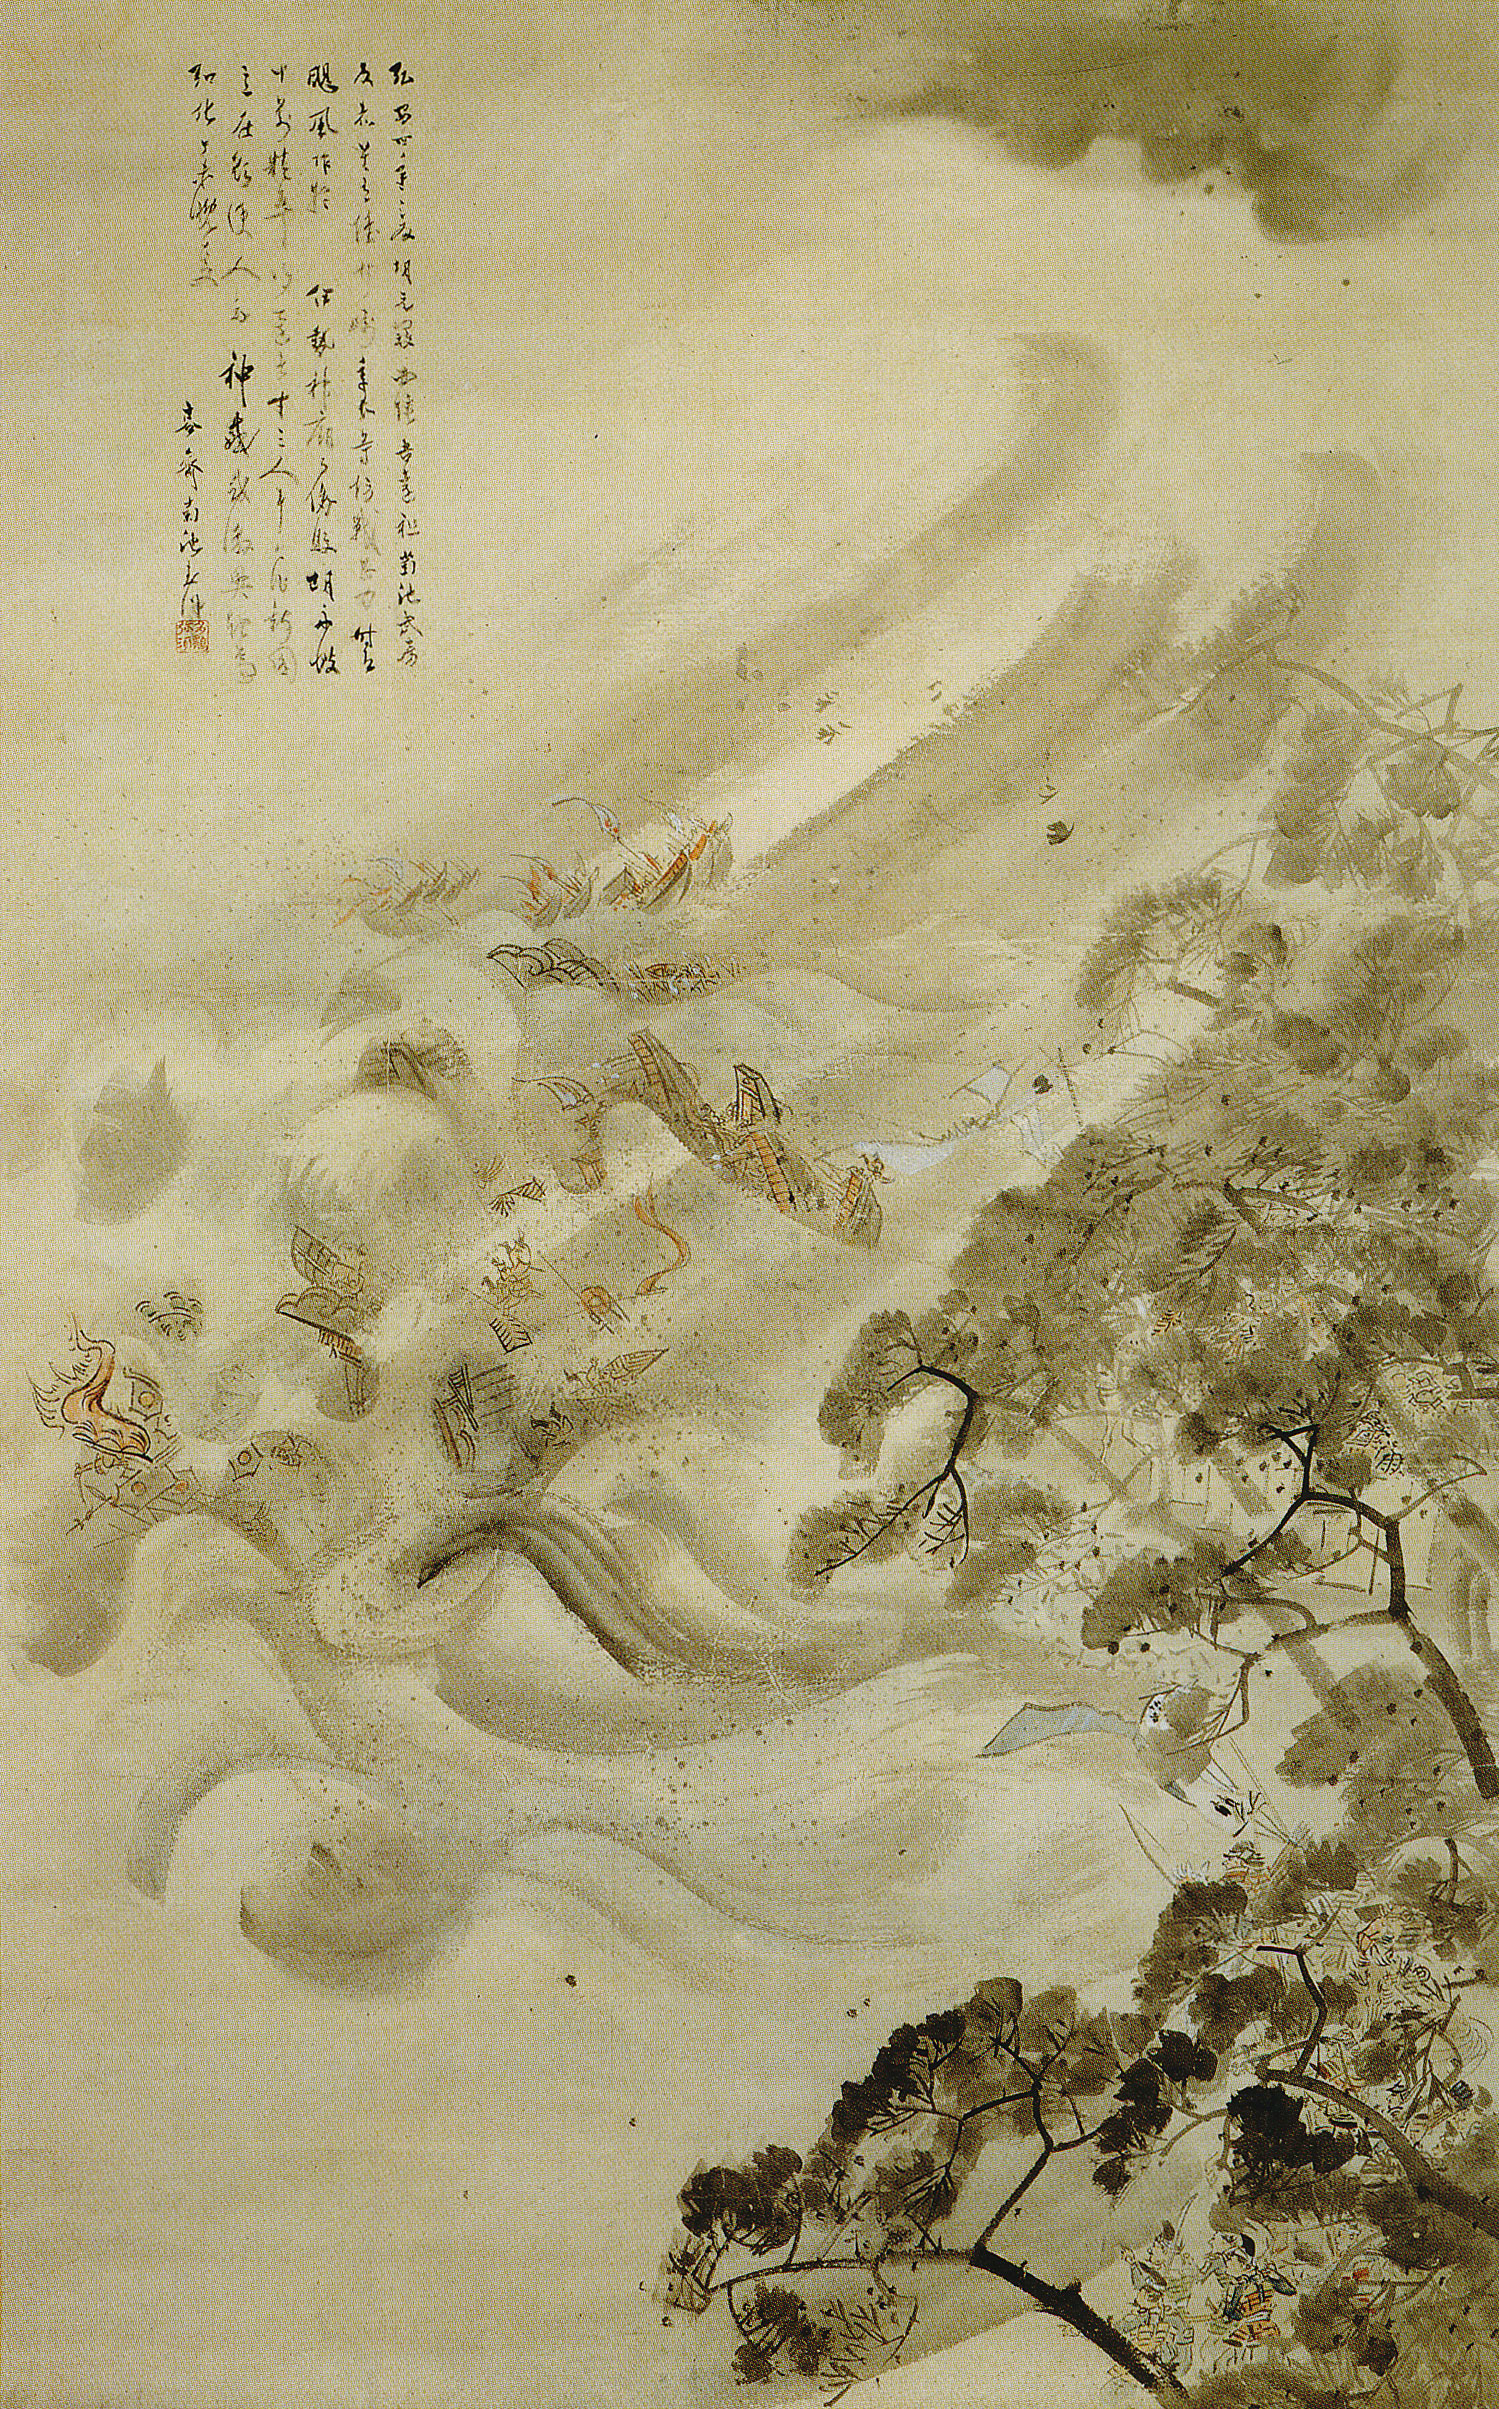
\includegraphics[width=0.34\textwidth]{MokoShurai.jpg}
    \caption{
        {\small
            The Mongol fleet destroyed in a typhoon, 1847. \textit{Source}: Kikuchi Y\={o}sai / 
            Tokyo National Museum (Public domain)
        } 
    }\label{fig:mongolJapan}
\end{wrapfigure}

\emph{Earth}, \emph{Wind}, \emph{Fire} \& \emph{Water}, the \emph{classical elements} were the 
basis for understanding our environment during antiquity. Modern science, based on experiments has 
taken a very different view of the world, one based on atoms, fundamental particles and states of 
matter. But we could argue that the classical elements were a more philosophical idea that 
distilled our everyday experiences with nature, in fact many ancient cultures such as 
Hellenistic Greece, Babylonia, Japan, Tibet, China and India had similar lists of four or five 
elements. These civilizations had very different views on the properties of these elements and how 
they related to natural phenomena, quite often these links were mythological. The obvious way in 
which people experienced the classical elements was through weather systems. 

From the seasons to daily variations, nature's elements drive and shape our lives. Sometimes 
weather has had a direct impact on entire populations, one example was the failed Mongol invasions 
of Japan in $1274$ and $1281$. In both attacks, the Mongol fleets were almost entirely destroyed by 
storms called \emph{kamikaze} (translates to divine wind). Although some attacking Mongol forces 
did manage to land during the $1274$ campaign and outnumbered the defending armies, they were still 
defeated by Samurai clans with superior knowledge of the terrain. 

The invading fleet of $1281$ was composed of \enquote{more than four thousand ships bearing nearly 
$140,000$ men} \citep[pg.~17]{mcclain2002japan}, the scale of which was eclipsed only by the allied 
invasion of Normandy in $1944$. The fleet was a hastily assembled, consisting of ships which were 
not suitable for the harsh waters between Japan and Korea. The Japanese had built two metre high 
walls in the intervening period and the invading fleets were forced to stay in sea for months. 
After their supplies were diminished, powerful kamikaze winds destroyed them entirely (an artist's 
view of the event is illustrated in \cref{fig:mongolJapan}). The failed invasions were a blow to 
the idea of Mongol supremacy in Asia and the Mongols never attempted an invasion of Japan since.

We now know that weather phenomena are caused by a combination of air pressure, temperature and 
moisture differences between one place and another. The angle of the Sun's rays changes with 
latitude, these variations create very different temperature trends from the poles to the equator. 
These differences in temperature lead to large scale air currents which create complex weather 
systems and climate patterns which we see across the world. But weather phenomena are hardly 
exclusive to planet Earth.

\section*{The Final Frontier}

\begin{wrapfigure}{r}{0.35\textwidth}
    \centering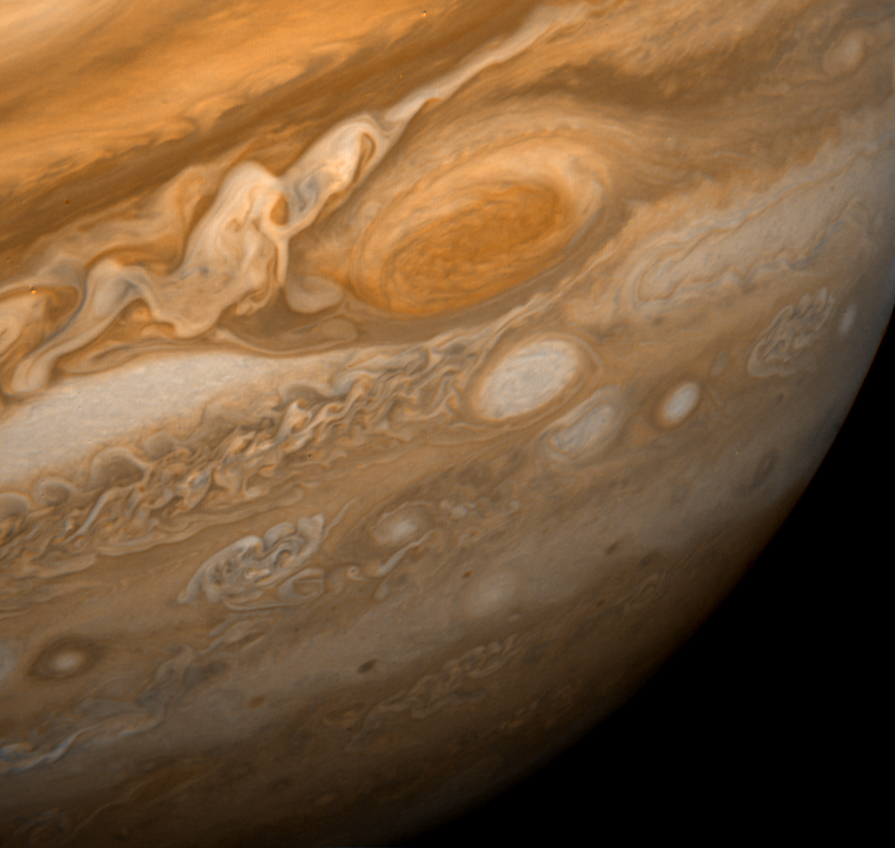
\includegraphics[width=0.38\textwidth]{Great_Red_Spot_From_Voyager_1.jpg}
    \caption{
        {\small 
            Jupiter's Great Red Spot in February $1979$, photographed by the unmanned 
            Voyager $1$ NASA space probe. \textit{Source}: NASA (Public domain)
        }
    }
    \label{fig:jupiter}
\end{wrapfigure}

Even before the beginning of the space age, weather phenomena occurring on other planets have been 
observed. Jupiter's \emph{great red spot}, a huge storm, has been continuously observed since 
$1830$ \citetext{see \citealp{britannicaRedSpot}}.

Saturn's \emph{great white spot}, a recurring storm system which was first used by Asaph Hall to 
determine the period of the planet's rotation \citep{wikisaturn}. In the $20^{\text{th}}$ century, 
missions such as the Hubble space telescope, Voyager, Cassini and others have shown storms and 
other weather phenomena on planetary bodies like Venus, Mars, Neptune and Titan. 

The principles behind many planetary weather phenomena are very similar. Each planet has a 
different atmosphere, so weather phenomena in the solar system can have very different 
characteristics. Extra-terrestrial weather is just as complex and mind boggling as weather we 
observe on Earth, its scale is certainly much larger than we are used to. 

Yet, planetary weather is just one side of the puzzle. Venturing into our cosmic neighbourhood, 
our solar system has another kind of weather system that has begun to be probed only very recently. 

\subsection*{A Gust of Wind from the Heavens}

During the last week of August $1859$, several spots appeared on the surface of the Sun. Southern 
auroral displays were observed on August $29$, as far north as Queensland Australia. Just before 
noon on September $1$, British astronomer Richard Carrington observed a \enquote{white light flare} 
from a group of sun spots. He created a sketch of his observations which is seen in 
\cref{fig:carringtonevent}. Carrington's observations were independently verified by British 
publisher and astronomer Richard Hodgson, both of them sent their reports to the 
\emph{Monthly Notices of the Royal Astronomical Society}.

September $1$-$2$ $1859$ saw some remarkable events occur around the world. Auroral displays were 
observed all around the world, even in low latitude places such as Colombia 
\citep{MORENOCARDENAS2016257}. Auroras above the rocky mountains in the U.S were so bright that 
they woke up gold miners who began preparing breakfast thinking it was morning \citep{miners}. In 
the northeastern U.S, people could read the newspaper by the aurora's light \citep{auroraReading}.

\begin{wrapfigure}{l}{0.5\textwidth}
    \centering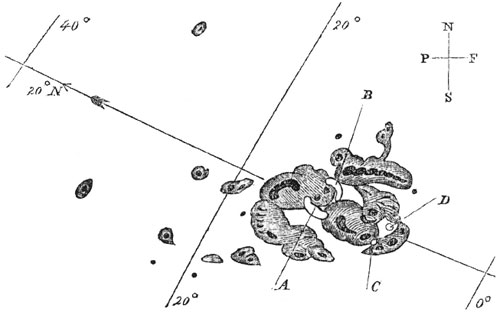
\includegraphics[width=0.48\textwidth]{Carrington_Richard_sunspots_1859.jpg}
    \caption{
        {\small
            Sunspots of September 1, 1859, as sketched by Richard Carrington. 
            A and B mark the initial positions of an intensely bright event, 
            which moved over the course of five minutes to C and D before 
            disappearing. \textit{Source}: Richard Carrington (Public domain)
        } 
    }
    \label{fig:carringtonevent}
\end{wrapfigure}

The telegraph network in Europe and North America failed. Some operators experienced electric 
shocks \citep[pg.~13]{board2008committee} while in some cases even telegraph equipment that was 
disconnected from the power supply could be used to transmit messages 
\citep[pg.~58]{carlowicz2002storms}.

Based on global reports and observations taken by Scottish physicist Balfour Stewart at the 
Kew observatory in London, Carrington was able to connect events observed on the Earth to what 
he saw on the Sun on the $1^{\text{st}}$ of September \citep{clark2007sun}. His assertion was 
corroborated by other observers in the scientific community.

The storm of $1859$, later known as the \emph{Carrington event} was in some ways the genesis of 
\emph{Space Weather}, although the actual term was coined much later in the $1950$s. Although 
scientists had observed sunspots and their links to magnetic field variations on the Earth earlier, 
the \emph{Carrington event} was a concrete example of how activity on the Sun could have 
potentially dramatic effects on the Earth.

\subsection*{Space Weather}

How do spots and ejections from the Sun produce bright lights and currents on Earth? During 
Carrington's time the fledgling science of electromagnetism had picked up in the $19^{\text{th}}$ 
century and already had some understanding of these phenomena. Faraday's induction experiment from 
$1831$ (\cref{fig:induction}) had shown that varying magnetic fields could induce electrical 
currents in copper wires.

\begin{figure}
    \noindent\centering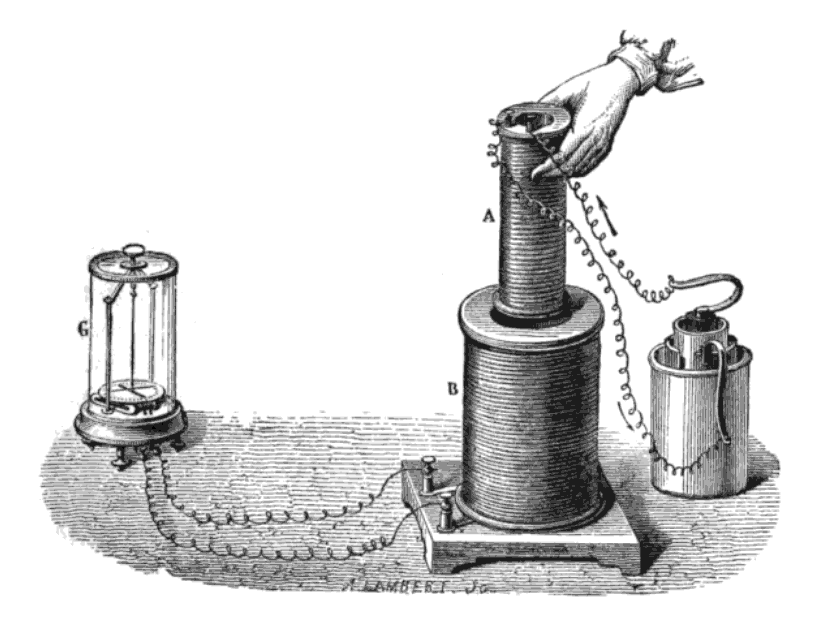
\includegraphics[width=0.7\textwidth]{Induction_experiment.png}
    \caption{
        {\small
            One of Faraday's $1831$ experiments demonstrating induction. 
            The liquid battery (right) sends an electric current through the small coil (A). 
            When it is moved in or out of the large coil (B), its magnetic field induces a 
            momentary voltage in the coil, which is detected by the galvanometer (G). 
            \textit{Source}: J. Lambert (Public domain)
        }
    }
    \label{fig:induction}
\end{figure}

It took approximately a century from the \emph{Carrington event} for a theoretical understanding of 
Space Weather phenomena to develop. Maxwells equations of Electromagnetism \citep{maxwell1865viii} 
published in $1864$ gave scientists the mathematical tools to model the motions charged particles 
in electric and magnetic fields and the variations in the fields themselves due to those moving 
particles.

The $20^{\text{th}}$ century saw rapid progress made in modelling of charged particles in the 
Earth's magnetic field in the area of \emph{plasma physics}, plasma was the name given to the state 
of matter which existed as an ionised gas. From the scientific advances made in space weather and 
plasma physics, we know that the Carrington white light flare in $1859$ was accompanied by a large 
release of energetic plasma from the Sun's atmosphere, also known as a \emph{coronal mass ejection} 
(CME). The CME associated with the Carrington event was particularly energetic and compressed the 
Earth's magnetic field causing currents to flow in conducting materials like telegraph equipment. 

Space weather started gaining relevance with the rise of space missions and satellites and the 
risks posed by space weather events to space faring assets, although there was still much progress 
to be made. This was especially important with increasing reliance on electronic appliances and 
communication networks.

\subsubsection*{Impacts}

The Quebec power grid failure of $1989$ \citep{kappenman1997geomagnetic} during a geomagnetic storm 
event showed that intense space weather events like the one observed in $1859$ could cause 
significant damage to communications, energy and technological infrastructure that so crucial to 
the functioning of modern civilization.

It is now widely accepted that space weather events can adversely impact satellite and 
communication infrastructure, airline industry, navigation systems and the electric power grid 
\citep{board2009severe,cannon2013extreme,bothmer2007space,baker2004effects}. To protect our 
technological systems and humans in deep space exploration, it is necessary to have an advance 
knowledge of the changes in space weather that can pose potential threats.

\subsubsection*{The Future}

The solar storms observed in the $20^{\text{th}}$ and $19^{\text{th}}$ centuries are only one 
part of the picture. It is now increasingly likely that private companies will be making 
significant inroads into space travel for business goals. Companies such as SpaceX and BlueOrigin 
aim to make space travel cheaper and more accessible so that human beings can live and work in 
space or other planets in the solar system, potentially starting a second space age.


\begin{wrapfigure}{l}{0.4\textwidth}
    \centering\includegraphics[width=0.38\textwidth]{spacex.jpg}
    \caption{
        {\small
            Artist's impression of the SpaceX Interplanetary Starship on the Jupiter's moon Europa 
            \textit{Source}: Space Exploration Technologies Corp. [CC0]
        } 
    }
    \label{fig:spacex}
\end{wrapfigure}

This drastic move to become a multi-planetary species will bring with it the risks to the human 
life and equipment. These risks come in the form of severe magnetic storms, solar flares and 
ejections of charged particles, which must be anticipated if we want to become a successful space 
faring race. 

In order to design resilient technological systems for the new space age, we need to make progress 
in understanding and anticipating space weather phenomena. Physical theories about space plasmas 
needed to be combined with the data collected from space missions. The rapid rise of hardware, 
software, data storage, the deluge of space mission data and the advent of machine learning 
techniques means that we are in a unique position to take strides towards our space goals.


%\bibliographystyle{plainnat}
%\bibliography*{references}


\clearemptydoublepage

\chapter{Preliminaries}\label{chapter:preliminaries}

\emph{Space weather} is the branch of physics that studies the time varying phenomena in the solar 
system. The principal driver of space weather phenomena is the Sun, specifically its magnetic field 
variations and the \emph{solar wind}. The effect of solar variations on the planetary environment 
are caused by the coupling between solar wind particles and the magnetic field produced by the 
Earth. This chapter gives a semi-quantitative treatment of various scientific ideas relevant to 
space weather research.

\begin{table}
    \centering
    \begin{tabular}{l p{0.35\textwidth} r}
        \hline
        \textbf{Chapters} & \textbf{Themes} & \textbf{Recommended Reading}\\
        \hline
        \vspace{5pt}
        \ref{chapter:dst_osa} \& \ref{chapter:dst_msa} & Forecasting of geomagnetic index $\mathrm{Dst}$. & \S~\ref{sec:geoindex}, \S~\ref{sec:mag}\textsuperscript{*}, \S~\ref{sec:plasma}\textsuperscript{*} \\
        \ref{chapter:bayes_diff_chapter} & Inference of radiation belt parameters. & \S~\ref{sec:plasmadiff}, \S~\ref{sec:plasma}\textsuperscript{*} \S~\ref{sec:mag}\textsuperscript{*} \\
        \ref{chapter:pdt} & Forecasting of near Earth solar wind speed using solar data. & \S~\ref{sec:hmfsolarwind}, \S~\ref{sec:sunspots}, \S~\ref{sec:solar}\textsuperscript{*}\\
        \hline
    \end{tabular}
    \caption{Dissertation Guide. {\small Asterisk\textsuperscript{*} denotes optional material.}}
    \label{table:chapterguide}
\end{table}

\Cref{table:chapterguide} provides the reader with a condensed guide to this dissertation. 
It connects the content presented in this chapter with the main research problems analyzed in the 
later chapters and provides recommended prerequisite reading for each chapter.

\Cref{sec:plasma} describes space plasmas and their properties. \Cref{sec:solar} provides some 
background about the Sun and the solar wind which is the driver for all space weather phenomena. 
This is used in the solar wind prediction task considered in \cref{chapter:pdt}. 
\Cref{sec:plasmadiff} introduces the plasma diffusion model (\cref{eq:fokker}) and its simplified 
radial diffusion system (\cref{eq:radialDiff}) which is used as the underlying physical model for 
\cref{chapter:bayes_diff_chapter}. \Cref{sec:mag} introduces the \emph{magnetosphere}, giving 
context for \cref{chapter:dst_osa,chapter:dst_msa}. 


\section{Space Plasma}\label{sec:plasma}

Plasma, also known as the fourth state of matter due to its properties that differentiate it 
from the conventional gaseous state, is ubiquitous throughout the visible Universe. Plasma is a gas 
which is composed of roughly equal number of positive and negatively charged particles, a property 
known as charge \emph{quasi-neutrality}. The term quasi-neutral is used because although the gas 
has almost equal amounts of positive and negative charges, the mixture is electromagnetically 
active. Due to incomplete charge shielding, long range electromagnetic fields play a big role in 
the dynamics of plasma.

%From classical electrostatics the electric potential of a point charge $q$, is given as

%\begin{equation}
%    \phi(r) = \frac{q}{4\pi\epsilon_0 ||r||_2}
%\end{equation}

%where $r$ is the position in space with respect to the charge and $\epsilon_0$ is the \emph{permittivity} of vacuum.

\subsection*{Debye Length}

In a quasi-neutral plasma, due to the presence of partial electric shielding the potential due to 
the charges now takes the well known Debye form
%
\begin{equation}
    \phi(r) = \frac{q}{4\pi\epsilon_0 r} e^{-\frac{r}{\lambda_d}} \ , 
\end{equation} 
%
where $r$ is the spatial distance with respect to the charge and $\epsilon_0$ is the 
\emph{permittivity} of vacuum. The electric potential decays with the Debye length scale 
$\lambda_d$ at which a balance between thermal vibrations which can disturb quasi-neutrality, and 
electrostatic forces due to charge separation, is achieved. The Debye length scale depends on the 
electron temperature and plasma density.
%
\begin{equation}\label{eq:debye}
    \lambda_d = \sqrt{\frac{\epsilon_0 k_b T_e}{n_e e^2}}
\end{equation}
%
In \cref{eq:debye} above, the Debye length scale is expressed in terms of the 
\emph{Boltzmann constant} $k_b$, the electron temperature $T_e$, free space permittivity 
$\epsilon_0$, and electron charge $e$. One can visualise the positively charged ions having a cloud 
of electrons shielding them at the distance of $\lambda_d$. 

It is also possible to take into account the shielding effect of the ions. The effective Debye 
length is now expressed as an addition of two terms: one for electrons (\cref{eq:debye}) and a 
similar term for the ions by replacing $T_e$ for the ion temperature $T_i$ ($n_i \approx n_e$). 

\subsection*{Plasma Parameter}

Consider a Debye sphere of radius $\lambda_d$. This sphere contains 
$N_e = \frac{4}{3}\pi \lambda^3_d n_e$ electrons. The plasma parameter $g$ is defined as 
$N_{e}^{-1}$. Rewriting this, we can say:
%
\[
    g \sim \sqrt{\frac{n_e}{T_e}} \ .
\]
%
The description of plasma used in many applications in space is applicable when $g \ll 1$. In 
this situation the Debye shielding is significant, and the quasi-neutral plasma obeys collective 
statistical behavior. The plasma parameter $g$ also correlates with the collision frequency. The 
collisions in plasma increase with increasing density and decreasing temperature, and if 
$g \longrightarrow 0$ the plasma becomes nearly collisionless. The collisionless property helps in 
making simplifying assumptions about plasma dynamics and serves as the starting point for the 
\emph{adiabatic} theory of plasma motions in the Earth's magnetosphere which will be discussed in 
\cref{sec:plasmadiff}.

\section{Sun \& the Solar Wind}\label{sec:solar}

\begin{figure}
    \noindent\centering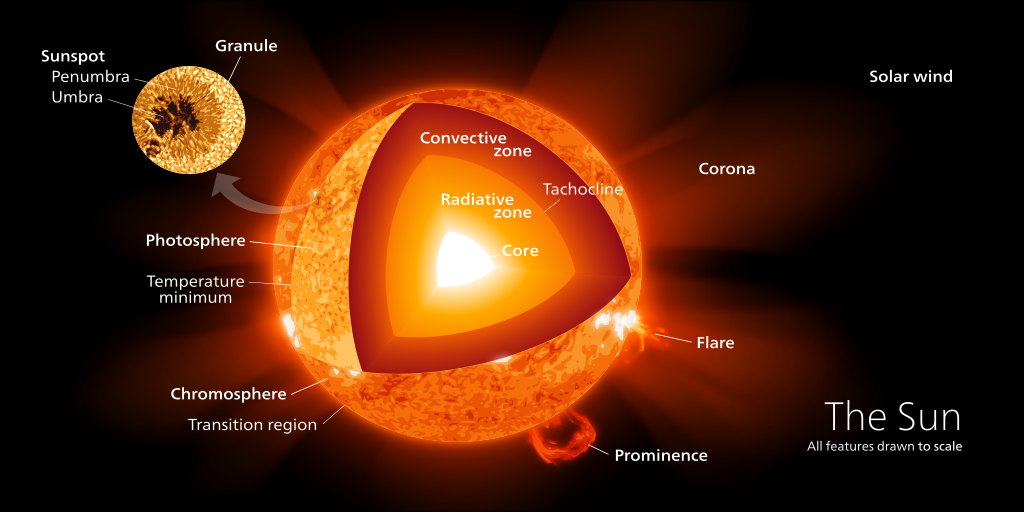
\includegraphics[width=\textwidth]{Sun_poster.png}
    \caption{{\small Cross section of the Sun \\ 
    Author: Kelvinsong [CC BY-SA 3.0 (\url{https://creativecommons.org/licenses/by-sa/3.0})]}}
    \label{fig:SunLayers}
\end{figure}

The Sun is an almost perfectly spherical ball of plasma which is the the center of our solar 
system and the only source of light and energy for all living and meteorological processes on 
Earth. Apart from terrestrial weather, the Sun is also the primary driver of space weather which 
results from the interaction between the solar wind and planetary magnetospheres.

\subsection{Structure}

\Cref{fig:SunLayers} shows a cross section of the Sun with various layers. We give a brief 
description of them below.

\textbf{Core}: The core of the Sun is the site for the thermonuclear fusion reactions which produce 
its energy. It extends from the center to about $20-25\%$ of the solar radius \citep{SolarAct}. It 
has a temperature close to $\SI{1.57d7}{\kelvin}$ and a density of 
$\SI{150}{\gram\per\centi\metre^3}$ \citep{SolarCore}. Nuclear fusion in the core takes place via 
the well known \emph{proton-proton chain} (pp).

\textbf{Radiative Zone}: The radiative zone extends from $25\%$ to $70\%$ of the solar radius. 
The nuclear reactions in the core are highly sensitive to temperature and pressure. In fact, they 
are almost shut off at the edge of the core. In the radiative zone, energy transfer takes place via 
photons (radiation) which bounce around nuclei until they reach the convective zone.

\textbf{Convective Zone}: The convective zone lies between $70\%$ of the solar radius to a point 
close to the solar surface. Density decreases dramatically going from the core to the radiative 
zone and subsequently the convective zone. In this region, the solar material behaves more like a 
fluid. Due to the temperature gradient which exists across it, the primary source of transport is 
here via convection.

\textbf{Photosphere}: The photosphere is the visible \enquote{surface} of the Sun, since the layers 
below it are all opaque to visible light. A layer of about $\SI{100}{\kilo\metre}$ thickness, the 
photosphere is also the region from where sunlight can freely escape into space. The photospheric 
surface has a number of features i.e. sunspots, granules and faculae. Sunspots 
(see \cref{sec:sunspots}) are magnetic regions where the solar material has a lower temperature 
compared to its surroundings. Magnetic field lines are concentrated in sunspot regions, and the 
field strength in sunspots can often be thousands of times stronger than the on the Earth.

% \begin{wrapfigure}{r}{0.4\textwidth}
%     \centering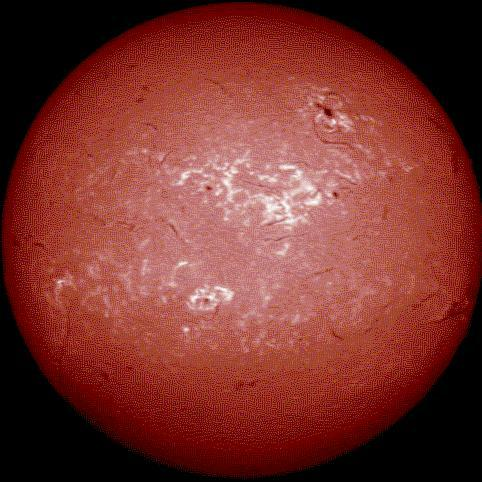
\includegraphics[width=0.38\textwidth]{chromosphere.jpg}
%     \caption{
%         {\small Chromosphere viewed using an $H\alpha$ filter. \\ \textit{Source}: CWitte (Public domain)}}
%     \label{fig:chromosphere}
% \end{wrapfigure}

\begin{wrapfigure}{r}{0.4\textwidth}
    \centering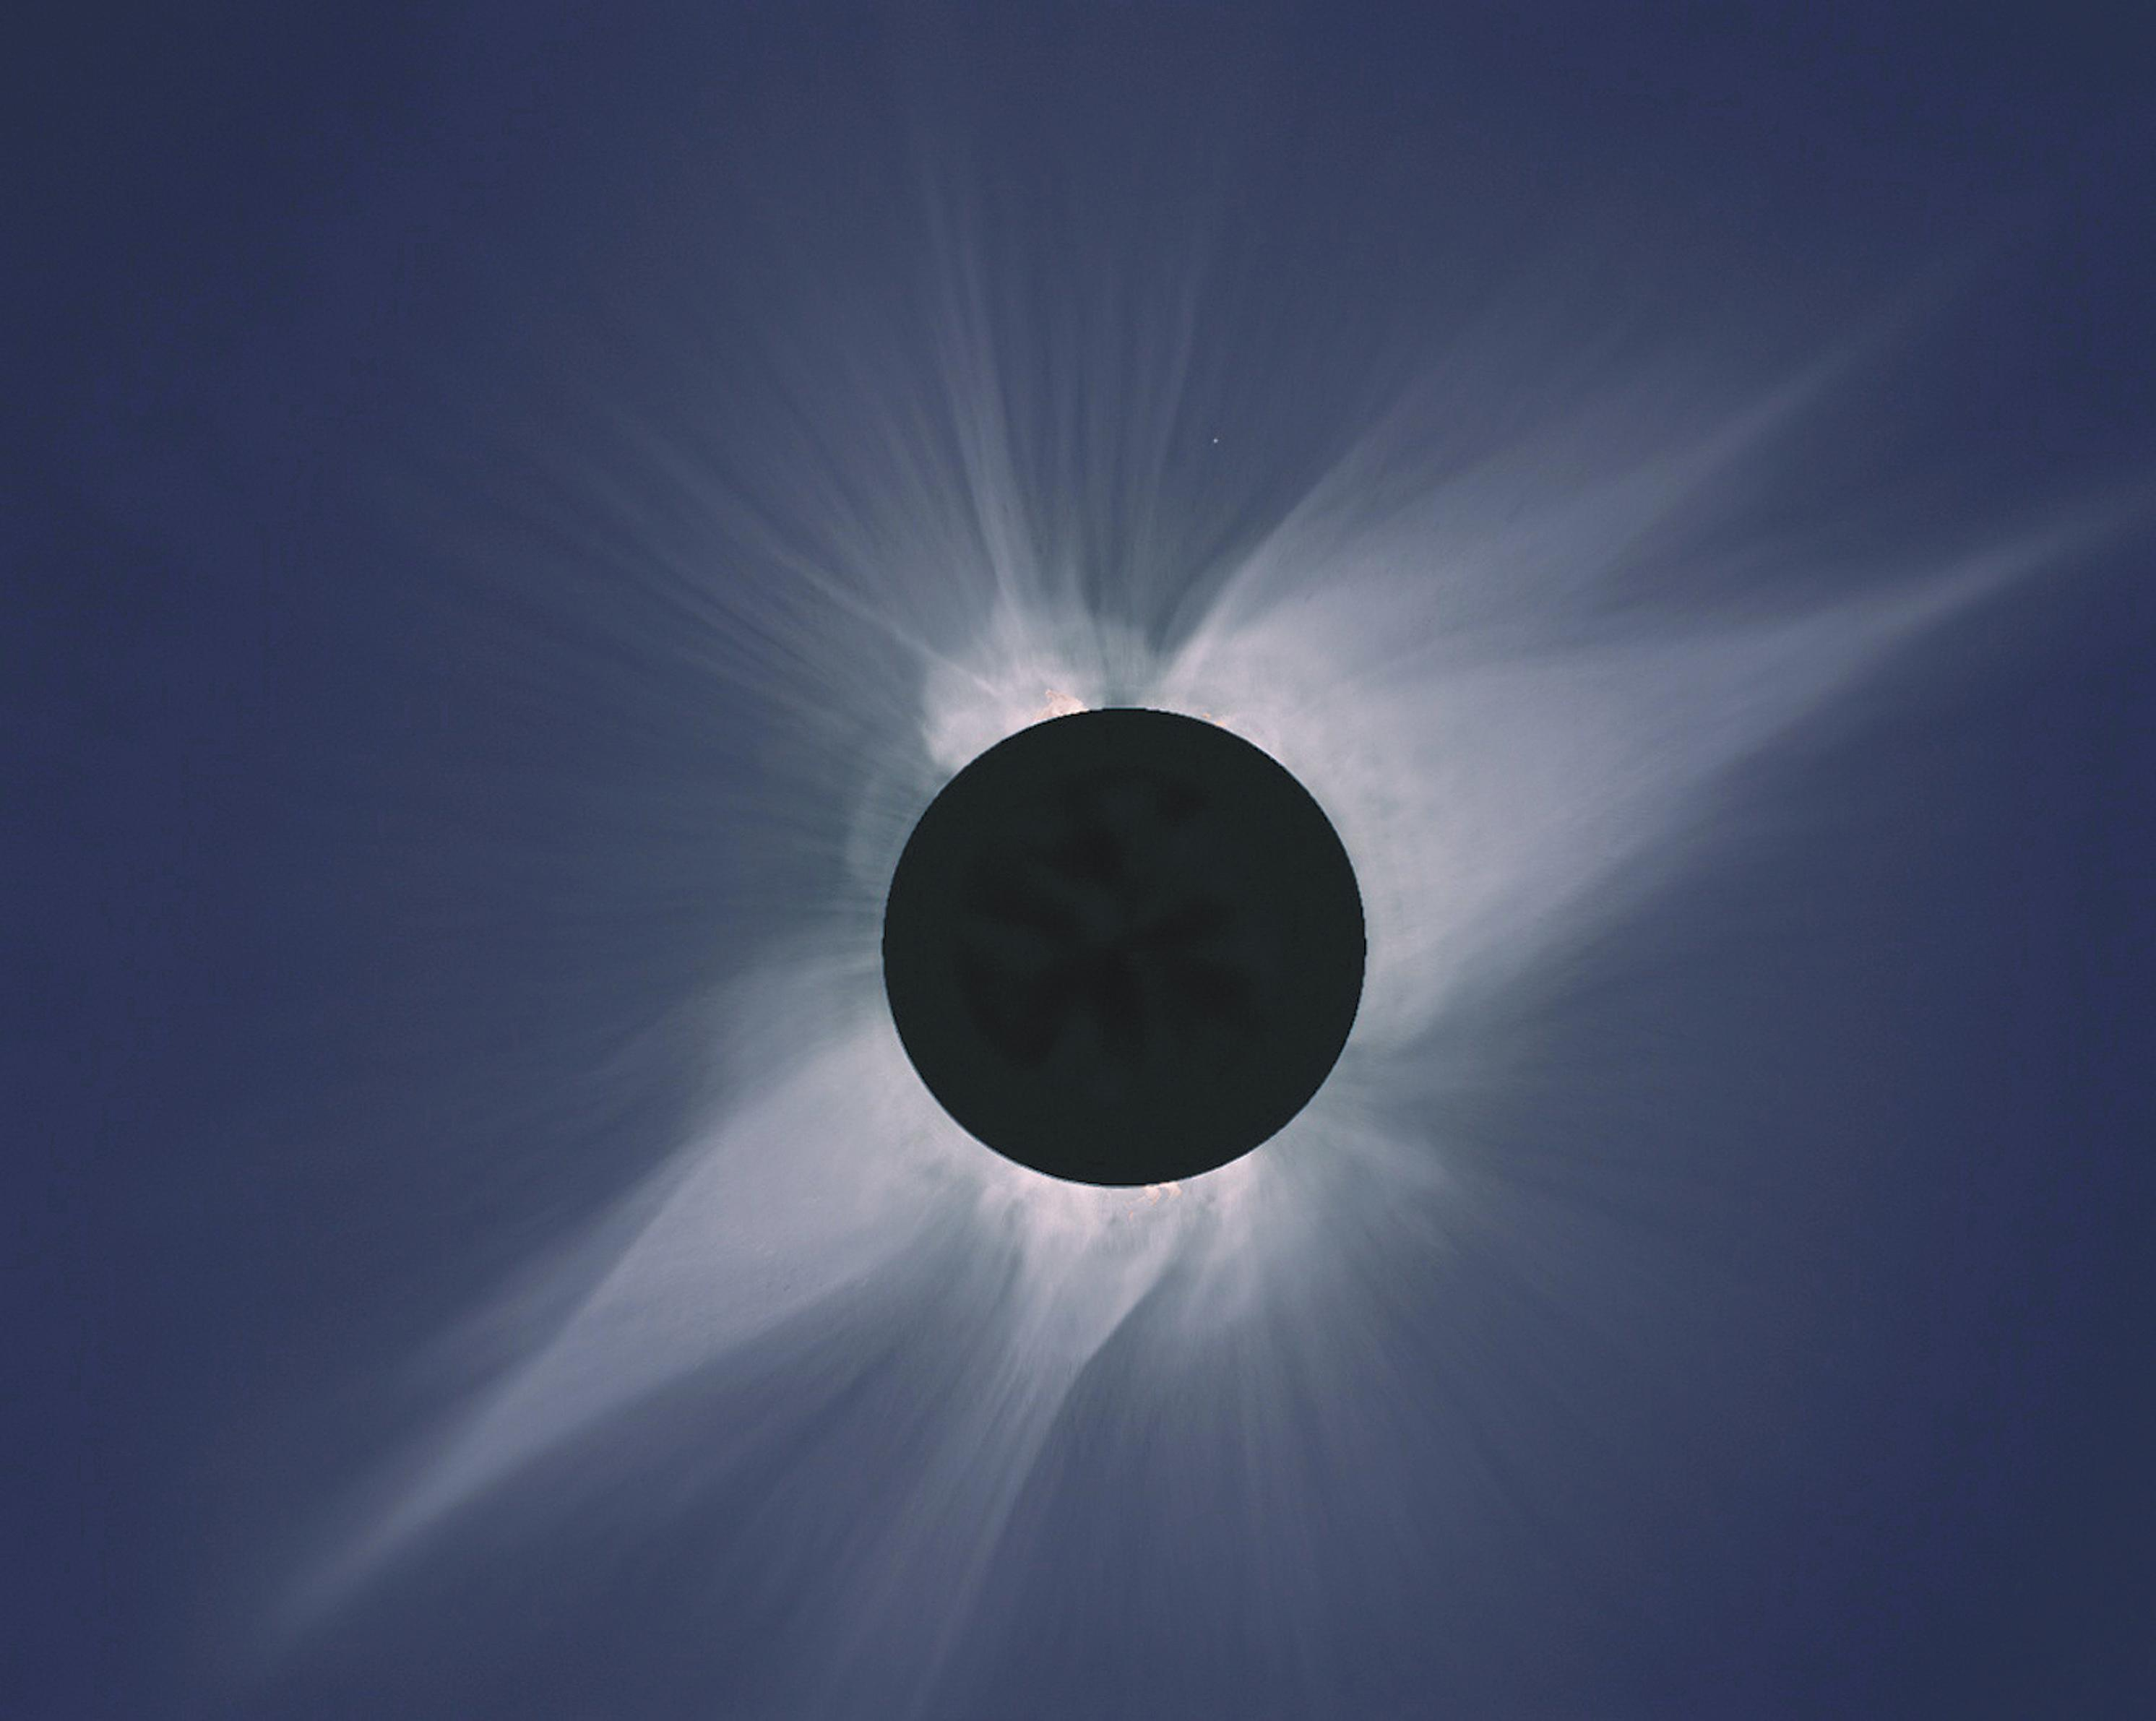
\includegraphics[width=0.38\textwidth]{coronaBaja.jpg}
    \caption{
        {\small 
            Sun's corona captured during a solar eclipse. \\ 
            \textit{Source}: Steve Albers, Boulder, CO; Dennis DiCicco, Sky and Telescope; 
            Gary Emerson, E. E. Barnard Observatory
        }
    }
    \label{fig:coronaBaja}
\end{wrapfigure}


\textbf{Chromosphere}: The Chromosphere extends for a distance of almost $\SI{5000}{\kilo\metre}$ 
after the photosphere. The chromosphere is known for the existence of features called spicules and 
prominences. The chromosphere has a red colour which is generally not visible due to the intense 
light given off by the photosphere but can be observed through a filter centered on the Hydrogen 
$H\alpha$ spectral line. %(see figure \ref{fig:chromosphere}). 

\textbf{Solar Transition Region}: A thin ($\SI{100}{\kilo\metre}$) region between the chromosphere 
and the solar corona where the temperature rises from about \SIrange{8000}{5d5}{\kelvin}, the solar 
transition region might not be well defined at all altitudes; however its existence is evidenced by 
a bifurcation of the dynamics of the solar plasma. Below the transition region, the dynamics is 
dictated by gas pressure, fluid dynamics, and gravitation while above the region, the dynamics is 
dictated more by magnetic forces.

\textbf{Corona}: An aura of plasma around the Sun that extends millions of kilometers into space, 
the corona can be observed during a total solar eclipse (\cref{fig:coronaBaja}) or with a 
coronagraph. The temperature of the corona is dramatically higher than the photosphere and 
chromosphere. The average temperature can range from \SIrange{1d6}{2d6}{\kelvin} while in the 
hottest regions it can be as high as $\SI{2d7}{\kelvin}$ \citep{SolarCorona}. Although the reason 
for this dramatic increase is still not well understood, there exist various explanations using 
concepts of magnetic reconnection \citep{russell2001solar,SolarCorona} and Alfv\'en waves 
\citep{AlfvenCorona}. There is a critical height in the corona, known as the \emph{source surface}, 
below which the magnetic field controls the plasma completely. Above it the plasma carries 
the magnetic field with it into the interplanetary medium.


\subsection{Solar Wind \& Heliospheric Magnetic Field}\label{sec:hmfsolarwind}

The idea that the Sun was ejecting charged particles outwards into space was first hinted at after 
the solar storm of $1859$ by Richard Carrington \citep{cliver20131859} and later by George 
FitzGerald \citep{meyer2007basics}. Arthur Eddington, in a footnote of an article about the comet 
Morehouse in $1910$, was the first to suggest the existence of the solar wind, without naming it so 
\citep{eddingtonFootnote}.

In the $1950\text{s}$, studies of the anti-solar orientation of the ion tails of Halley's comet 
led to the theory of solar corpuscular emission \citep{Bierman1,Bierman2,Bierman3}. 
\citet{parker1958dynamics,Parker1960,Parker1965} argued that the corona cannot remain in 
hydrostatic equilibrium and that supersonic expansion of the corona is responsible for the 
outward expulsion of charged particles, which the author referred to as the \emph{solar wind}.

\citet{parker1958dynamics} also proposed a spiral model for the \emph{Heliospheric Magnetic Field} 
(HMF) and suggested that the solar wind carried with it the solar magnetic field. The Parker model 
was further supported its ability to explain the effect of the HMF on the modulation of galactic 
cosmic rays and their measured intensities close to the Earth \citep{ParkerSolarWind}. In $1959$ 
the Soviet spacecraft Luna $1$ was the first to directly observe the solar wind and measure its 
strength \citep{harvey2007russian}. Subsequently, the Mariner $2$ mission recorded properties of 
the positive ion component of the solar wind and confirmed the Parker spiral HMF model 
\citep{neugebauer1966mariner}.

The structure of the HMF is central to explaining the formation and propagation of the solar wind. 
The HMF in steady state points radially outward and rotates with the Sun, producing an 
\emph{Archimedean spiral} structure as postulated in \cite{parker1958dynamics} and shown 
schematically in \cref{fig:parkerspiral}. Photospheric observations of the magnetic field (see 
Global Oscillation Network Group \url{https://gong.nso.edu}) are often extrapolated to compute 
approximations to the coronal HMF topology. There exist a number of techniques used to perform such 
extrapolations: potential field based methods such as \emph{Potential-Field Source Surface} (PFSS) 
\citep{schatten1969model,altschuler1969magnetic}, PFSS variants such as 
\emph{Potential-Field Current Sheet} (PFCS) \citep{schatten1971current}, 
\emph{Current-Sheet Source Surface} (CSSS) \citep{csss}, and several others. Apart from potential 
based models, there exist more involved techniques based on Magnetohydrodynamics (MHD) such as 
\emph{Magnetohydrodynamics Around a Sphere} (MAS) \citep{linker1999magnetohydrodynamic}, 
ENLIL \citep{ODSTRCIL1996,ODSTRCIL1999a,ODSTRCIL1999b,ODSTRCIL2003,ODSTRCIL2004} and EUHFORIA 
\citep{pomoell2018euhforia}. 

The HMF can be seen as a combination of two components: the poloidal magnetic field and the 
toroidal magnetic field. The two fields often exchange energy between themselves over the course of 
several years in a cyclical phenomenon known as the \emph{solar cycle} 
(\cref{sec:sunspots}). Interested readers can read \citet{Owens2013} for an in-depth review on the 
phenomena that drive the HMF.

\begin{figure}
    \noindent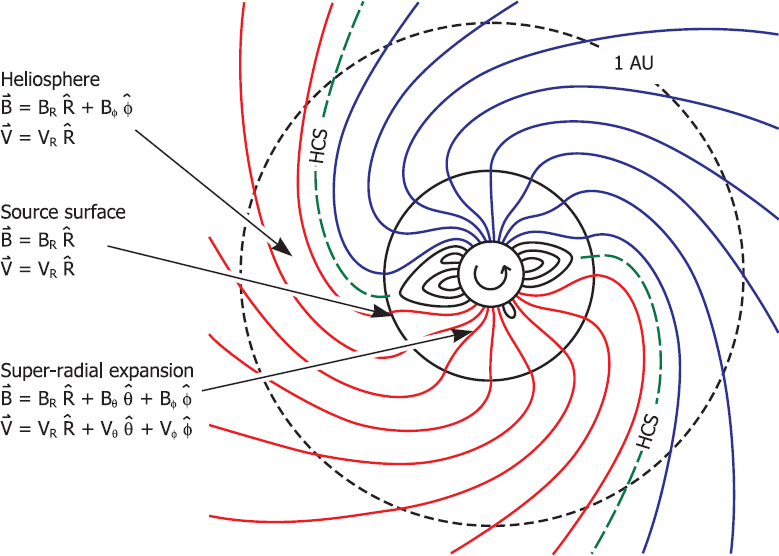
\includegraphics[width=0.8\textwidth]{parker-spiral.jpg}
    \caption{
        {\small 
            An illustration of the Heliospheric Magnetic Field in the \emph{ecliptic plane}. In the 
            heliosphere, rotation of the HMF foot points within a radial solar wind flow generates 
            an azimuthal component of the HMF, $B_{\phi}$, leading to a spiral geometry. Red and 
            blue lines, showing regions of opposite polarity, are separated by the heliospheric 
            current sheet (HCS), shown as the green dashed line. Image reproduced from 
            \citet{Owens2013}
        }
    }\label{fig:parkerspiral}
\end{figure}


The expansion of the coronal magnetic field leads to an eventual opening of field lines at the 
source surface (see \cref{fig:parkerspiral}) and the ejection of the solar wind. This hot plasma 
consists mostly of protons, electrons and a small number of helium and heavy ions. The solar wind 
spirals outwards in all directions, carrying with it the magnetic field. Close to the Earth's 
magnetosphere, this wind has a nominal speed of about $\SI{400}{\kilo\metre\per\second}$ while its 
high speed component has an average velocity of $\sim \SI{700}{\kilo\metre\per\second}$ 
(\cref{fig:solarwinddist}).

\begin{figure}
    \noindent\centering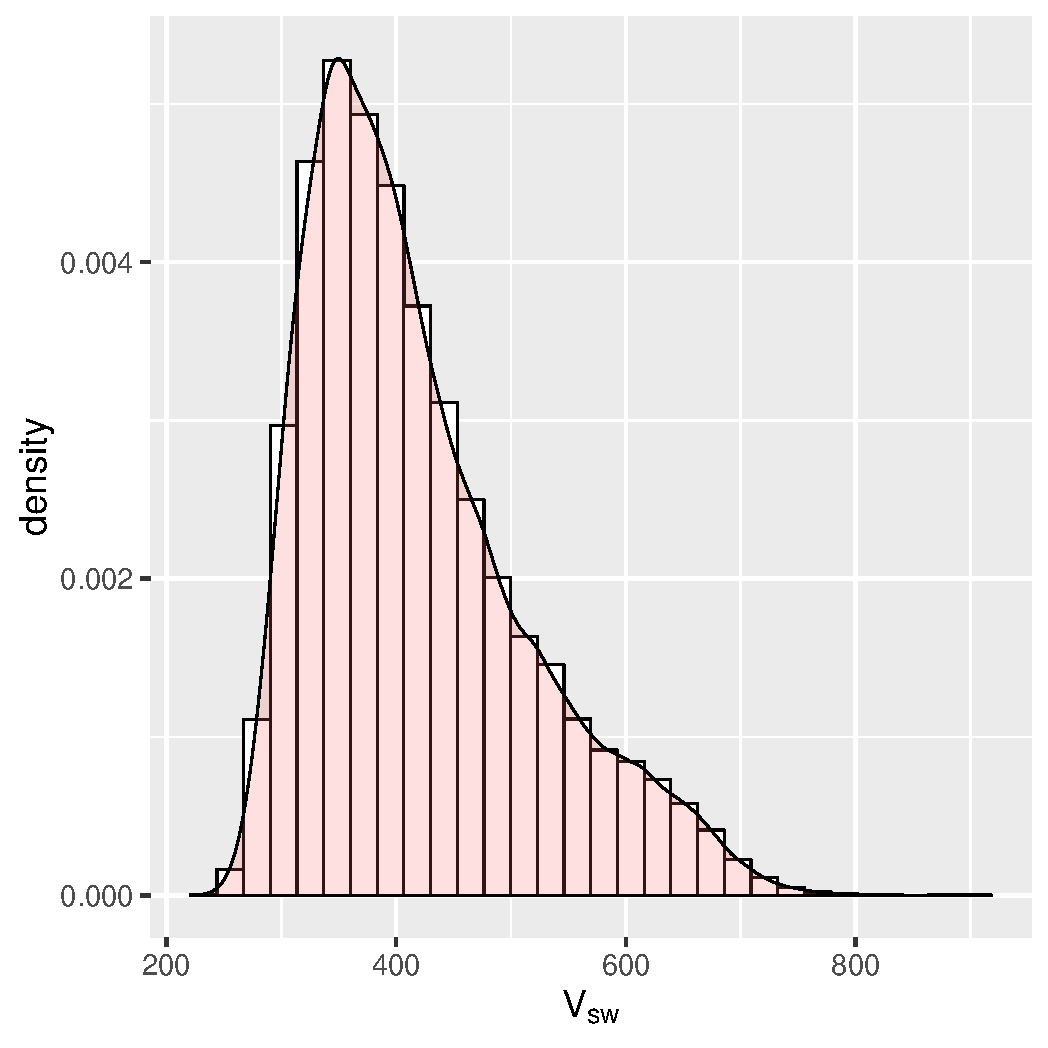
\includegraphics[width=0.75\textwidth]{solarwinddist.pdf}
    \caption{
        {\small 
            Distribution of solar wind speed recorded at $\SI{1}{\astronomicalunit}$ for the time 
            period $2008 - 2018$, \textit{Source}: OMNI data set 
            (\url{https://omniweb.gsfc.nasa.gov/ow.html})
        }
    }\label{fig:solarwinddist}
\end{figure}

\subsubsection*{Near Earth Measurements}

The solar wind has the heliospheric magnetic field \emph{frozen in} \footnote{the flux of the 
magnetic field going through a surface that moves with the solar wind (in a Lagrangian manner) is 
constant}, and as it propagates in the interplanetary medium, it carries the solar magnetic field 
with it \citep{alfven1942existence,alfven1943existence}. Important solar wind quantities such as: 
%
\begin{enumerate*} 
    \item solar wind speed, 
    \item proton density, and  
    \item magnetic field strength 
\end{enumerate*}
% 
are recorded at the well known $L1$ \emph{Lagrangian point} where the gravitational fields of the 
Earth and the Sun approximately balance out.



\subsection{Sunspots \& Solar Cycle}\label{sec:sunspots}

Sunspots are temporarily occurring regions on the Sun's photosphere that appear as dark spots. 
They are areas of magnetic field concentration where the field lines often \enquote{puncture} the 
solar surface inhibiting convection and producing regions with lower temperatures than the 
surroundings. Sunspots generally last anywhere between a few days to a few months. They can occur 
in pairs or groups and can accompany other phenomena such as \emph{coronal loops}, 
\emph{prominences}, and reconnection events.

Since the $19^{\text{th}}$ century the number of sunspots on the Sun's surface have been recorded 
as the \emph{sunspot number} (SSN). Sunspots populations increase and decrease, thereby behaving as 
markers for solar activity levels. The cyclical behavior of sunspot populations is called the 
\emph{sunspot cycle} or \emph{solar cycle} (\cref{fig:SolarCycle}). 

\begin{figure}
    \noindent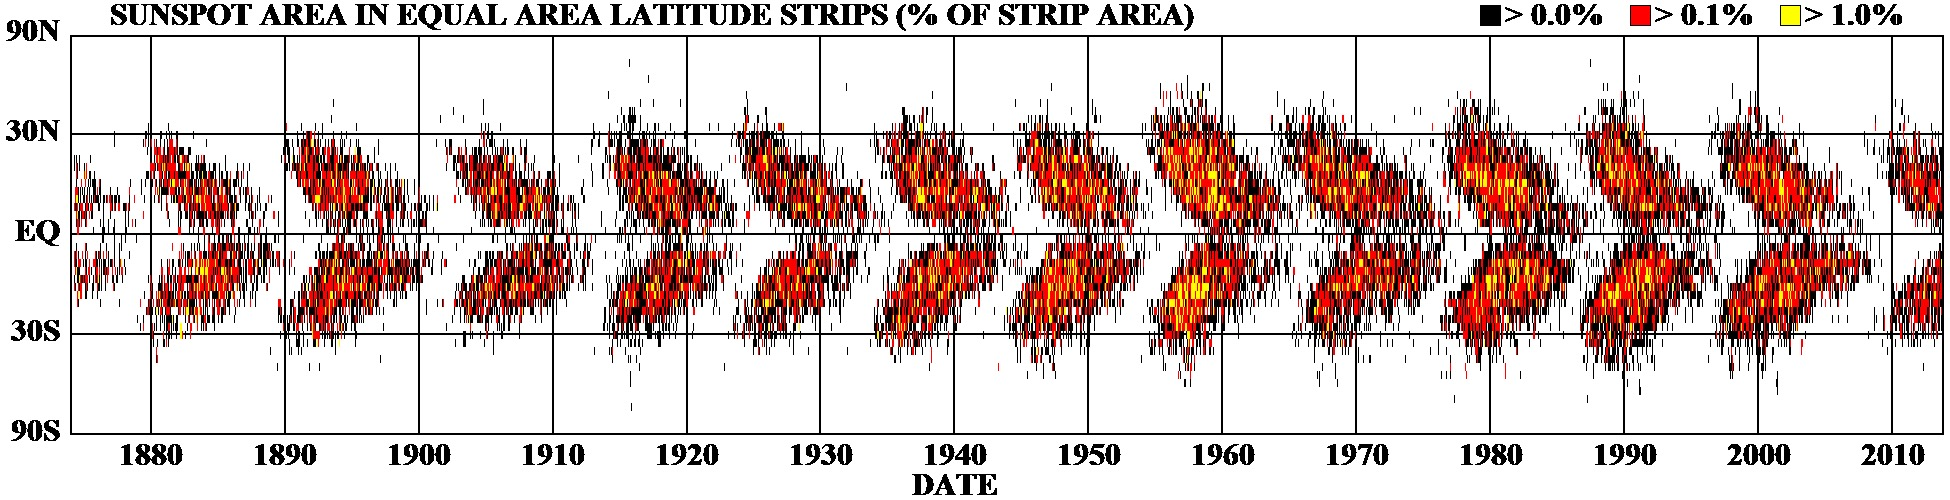
\includegraphics[width=\textwidth]{sunspot-cycle.jpeg}
    \caption{{\small The sunspot butterfly diagram.  \\ 
    \textit{Author}: David Hathaway, NASA, Marshall Space Flight Center (Public domain) \\ 
    \textit{Source}: Wikipedia}}
    \label{fig:SolarCycle}
\end{figure}

\Cref{fig:SolarCycle} depicts how the area occupied by sunspots changes with solar latitude 
and time. During the start of a solar cycle (solar minimum), sunspots start appearing at higher 
latitudes. Over the course of the cycle, they move towards the equatorial regions and their number 
increases to some maximum (solar maximum). Towards the end, the number of sunspots diminishes and 
the entire cycle starts over. This repetitive behavior happens over approximately $11$ years.

Because sunspots are magnetic phenomena, the solar cycle represents cyclical behavior of the HMF. 
During solar minimum, the poloidal component of the solar magnetic field is at its strongest and it 
is the closest it can get to a magnetic dipole configuration. Towards solar maximum, energy is 
transferred from the poloidal component to the toroidal component, resulting in complex field 
configurations which are evidenced by larger numbers of sunspot clusters.

The solar cycle also gives rise to variations in solar irradiance \citep{solarirradiance}. Between 
$1645$ and $1715$, very few sunspots were observed, a period known as the \emph{Maunder minimum}. 
This coincided with lower than average temperatures in Europe, which was called the 
\emph{little ice age}. Although the Maunder minimum was a period of lower solar irradiance, 
recent research \citep{owens2017maunder} has demonstrated that this was neither the only factor 
nor the most significant in causing lower than average temperatures during the little ice age.

In \cref{chapter:pdt}, the \emph{sunspot number} data as well as the \emph{flux tube expansion} 
factor ($f_S$ or FTE) and the magnetic field strength computed by the CSSS model will be used to 
create a input data set for building the \emph{dynamic time lag regression} model proposed therein. 
Using the input parameters, the \XX \ model provides an estimate for the near Earth solar wind 
speed as well as the propagation time. Measurements of the solar wind speed will also be used in 
\cref{chapter:dst_osa,chapter:dst_msa} as inputs to the Dst forecasting models applied therein.


\section{Magnetosphere}\label{sec:mag}

% \begin{figure}
%     \noindent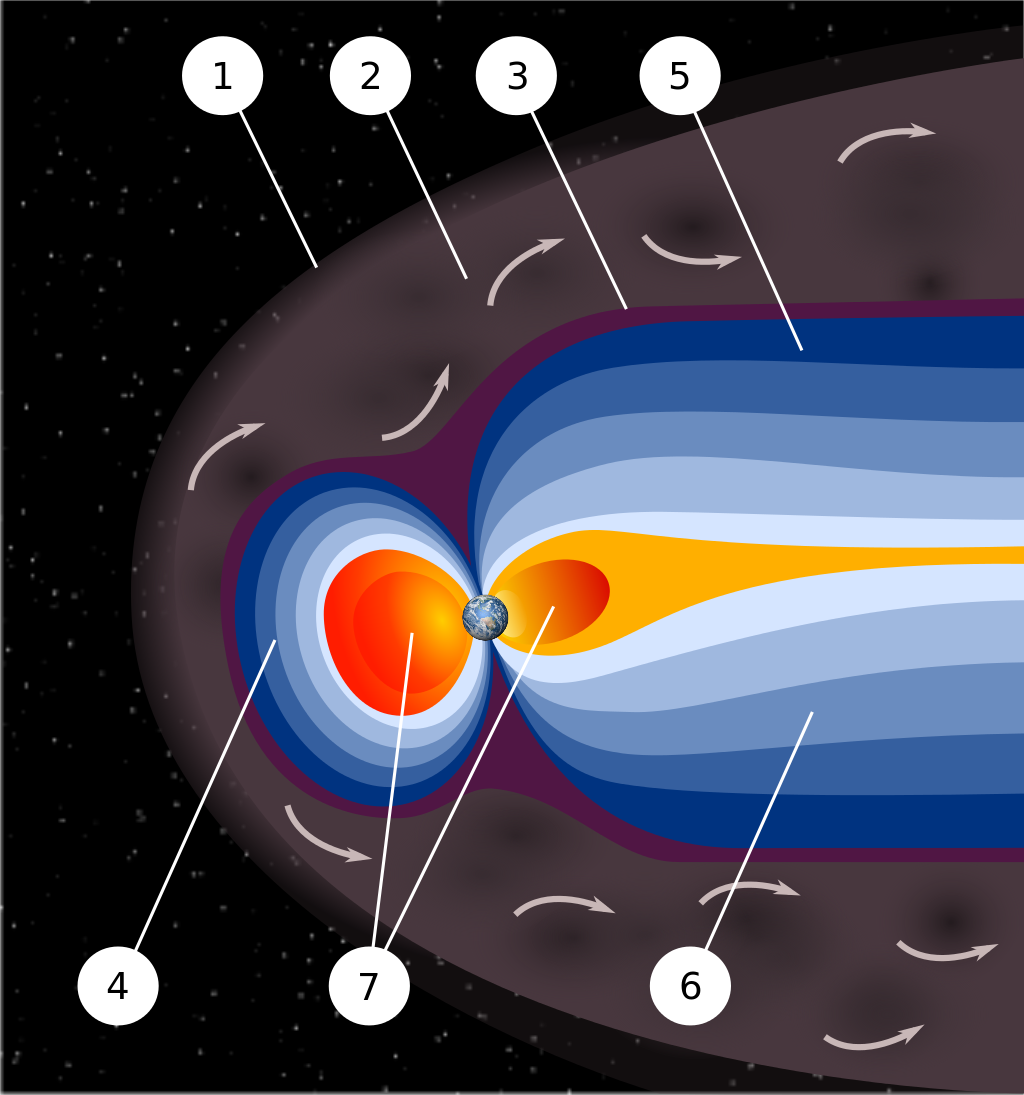
\includegraphics[width=0.7\textwidth]{mag.png}
%     \caption{{\small Schematic diagram of the Earth's magnetosphere: \\
%     The Sun (not shown) is to the left of the figure, the solar wind propagates from left to right.\\
%     1) Bow shock. 2) Magnetosheath. 3) Magnetopause. 4) Magnetosphere. \\
%     5) Northern tail lobe. 6) Southern tail lobe. 7) Plasmasphere.\\ 
%     Source: Dennis Gallagher, derivative work: Fr\'ed\'eric Michel (Public domain)}
%     }
%     \label{fig:magnetosphere}
% \end{figure}

\begin{figure}[ht]
    \noindent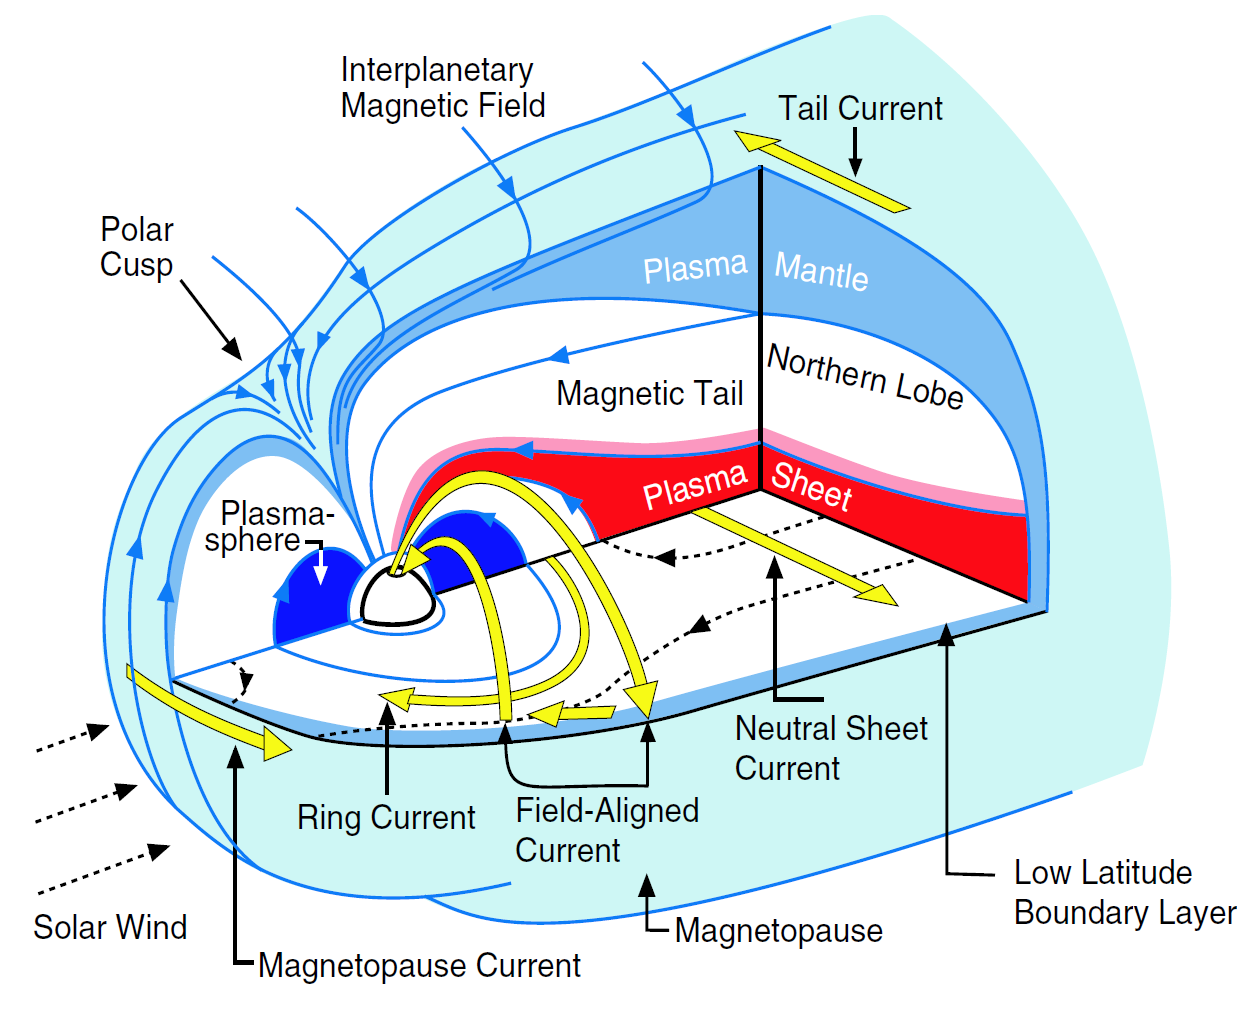
\includegraphics[width=0.8\textwidth]{mag3.png}
    \caption{
        {\small 
            Three-dimensional cutaway view of the magnetosphere. The light blue outer surface is 
            the magnetopause, and its boundary layers are shown in darker blue. Magnetic field lines 
            are shown in blue, electric currents in yellow. The polar region where the magnetic 
            field lines converge is the polar cusp. The bow shock has been omitted for clarity. 
            Image reproduced from \citet{DeKeyser2005}.
        }
    }
    \label{fig:magnetosphere}
\end{figure}

The Earth's magnetosphere (\cref{fig:magnetosphere}) is a region surrounding the planet where its 
magnetic field dominates the \emph{interplanetary magnetic field}. The Earth's magnetic field 
shields the atmosphere and terrestrial life from the impact of the solar wind. 

As the solar wind approaches the Earth, it is slowed down and deflected by the Earth's magnetic 
field. Since the solar wind is supersonic when it arrives and slows down to subsonic levels, a 
shock wave is generated in the process (\emph{bow shock}). Much of the solar wind kinetic energy is 
converted to thermal energy when it crosses the \emph{bow shock} into the \emph{magnetosheath}. The 
\emph{magnetosheath} spans from the \emph{bow shock} to the \emph{magnetopause}. The 
\emph{magnetopause} is the outer boundary of the Earth's magnetic shield. Its location is 
$\sim 10R_E$ ($R_E = \SI{6372}{\kilo\metre}$, the radius of the Earth). 


Earth's magnetic shielding is not perfect, and some particles manage to get trapped inside the 
cavity of the \emph{magnetosphere}. This region of trapped plasma is known as the the 
\emph{van Allen radiation belts}. Particles trapped in the radiation belts execute complex motions 
which can be approximately modelled using ideas from adiabatic theory and diffusion described in 
\cref{sec:plasmadiff} below. The \emph{plasmasphere} is the inner region of the radiation 
belts which contains cold, dense plasma. The portion of the magnetosphere facing away from the Sun 
(called the \emph{nightside}) is stretched out in a tail-like shape by the deflected solar wind, 
hence referred to as the \emph{magnetotail}. The \emph{magnetotail} has an approximate extent 
of up to $1000R_E$.


\subsection{Particle Motions \& Adiabatic Theory} \label{sec:plasmadiff}

This section gives a quick introduction to the theory of charged particle motions in the 
magnetosphere. The reader may refer to \citet{roederer2012dynamics} for an in depth treatment of 
this subject. To understand the motions of charged particles in the \emph{magnetosphere}, the role 
of electric and magnetic forces must be understood.

It is well known from classical electromagnetism that the force exerted on a particle with charge 
$q$ by a magnetic field $\mathbf{B}$ and an electric field $\mathbf{E}$ is given by the well known 
\emph{Lorentz force} (\cref{eq:lorentzforce}).
%
\begin{equation}\label{eq:lorentzforce}
    \mathbf{F} = m\frac{d\mathbf{v}}{dt} = q\mathbf{E} + q\mathbf{v} \times \mathbf{B}
\end{equation}
%
The first component of \cref{eq:lorentzforce} ($q\mathbf{E}$) is either parallel or opposite to the 
local electric field depending on the charge of the particle. The second component 
$q\mathbf{v} \times \mathbf{B}$ involves a vector cross product so it is always perpendicular to 
the plane spanned by vectors $\mathbf{v}$ and $\mathbf{B}$. In order to understand its effects, we 
can decompose the particle velocity in two components; $v_{\parallel}$ parallel to $\mathbf{B}$ and 
$v_{\perp}$ perpendicular to $\mathbf{B}$. If $\mathbf{E} = \mathbf{0}$, then the particle executes 
a circular motion with properties shown in \cref{eq:larmor}. Here $\rho$ is the gyroradius and 
$\omega$ is the gyrofrequency or cyclotron frequency. In the case where $v_{\parallel} \neq 0$, the 
trajectory is helical.
%
\begin{equation}\label{eq:larmor}
    \frac{v^{2}_{\perp}}{\rho} = \frac{qBv_{\perp}}{m} = \omega v_{\perp}
\end{equation}
%
Apart from the gyro motion, there are some important drift forces that significantly influence 
particle motions.
%
\begin{itemize}
    \item Electric field drift: If $\mathbf{E}$ has a component $E_{\perp}$ perpendicular to 
    $\mathbf{B}$, the electric field accelerates and decelerates the particle in the two 
    hemispheres of the orbit. The orbit becomes a distorted circle, and the particle drifts in a 
    direction perpendicular to the electric field with a velocity 
    $\mathbf{v_d} = \mathbf{E} \times \mathbf{B} / B^2$.

    \item Magnetic gradient drift: When the magnetic field varies in space (as is the case of the 
    Earth), a gradient in the field strength in the direction perpendicular to $\mathbf{B}$ gives 
    rise to a gradient drift velocity given by 
    $\mathbf{v_g} = \frac{1}{2} m v^2_{\perp}\mathbf{B} \times \frac{\nabla \mathbf{B}}{aB^3}$.

    \item Magnetic curvature drift: If the magnetic field has a curvature, this creates an 
    additional drift motion with velocity 
    $\mathbf{v_c} = \frac{ m v_{\parallel} \mathbf{B} \times (\hat{\mathbf{b}} \cdot \nabla) 
    \hat{\mathbf{b}} }{qB^2}, \ \ \mathbf{b} = \frac{\mathbf{B}}{B}$.
\end{itemize}

The equations of motion for charged particles in the general case of spatially varying electric and 
magnetic fields do not admit closed-form solutions. The motions are generally complex and require 
lengthy numerical integrations to be resolved.
%
\begin{figure}[ht]
    \centering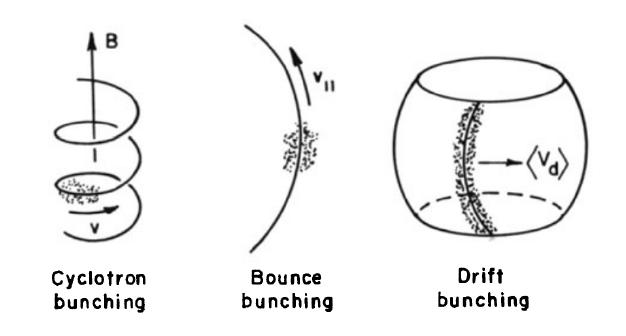
\includegraphics[width=0.4\textwidth]{adiabatic_motions.jpeg}
    \caption{
        {\small 
        The periodic components of the motion of trapped particles. Reproduced from 
        \citet{roederer2012dynamics}
        }
    }
    \label{fig:particlemotions}
\end{figure}
%
\todo{\textbf{TODO}: Check that the adiabatic motion image from Roederer can be reproduced here.}

The \emph{guiding center} approximation helps us to decompose particle motions into three periodic 
components (\cref{fig:particlemotions}):
%
\begin{enumerate*}
    \item gyration around magnetic field lines, 
    \item bounce motions between magnetic north and south poles, and
    \item equatorial drift of electrons and protons, 
\end{enumerate*}
%
each with its own time scale.

\subsubsection*{Adiabatic Invariants}

When a physical system with periodic motion is varied slowly as compared to the time period of 
its periodicity, the transformation can be characterized as \emph{adiabatic}. 
Formally speaking, for systems which are described by Hamiltonian dynamics, we can write the 
equations of motion in terms of the \emph{canonical position} $q$, the \emph{canonical momentum} 
$p$, external parameters $\theta$, and the system's \emph{Hamiltonian} $\mathcal{H}(q,p|\theta)$: 
%
\begin{equation}\label{eq:hamilton}
    \begin{aligned}
        \dot q &= \frac{\partial \mathcal{H}}{\partial p}\\
        \dot p &= - \frac{\partial \mathcal{H}}{\partial q} \ .
    \end{aligned}
\end{equation}
%
If the system shown in \cref{eq:hamilton} executes a periodic motion in the $q,p$ phase 
space, it admits an \emph{adiabatic invariant} $A$ given in \cref{eq:adiabatic_invariant}.
%
\begin{equation}\label{eq:adiabatic_invariant}
    A = \oint p d q
\end{equation}
%
The quantity $A$ would remain approximately constant if the external parameters $\theta$ were 
varied adiabatically (i.e. if changes in $\theta$ happen over a time period much greater than 
the period of oscillation of the system).

Applying the idea of adiabatic invariance to charged particle motion in the \emph{magnetosphere}, 
it is possible to associate one adiabatic invariant with each periodic motion i.e. gyromotion 
$\mathcal{M}$, bounce $J$, and drift $\Phi$ (\cref{eq:plasmainv}). 
%
\begin{align}\label{eq:plasmainv}
    \mathcal{M} &= \frac{1}{2}\frac{mv^{2}_{\perp}}{\rvert \mathbf{B} \rvert} \\
    J &= \oint{m_0 v_{\parallel}ds} \\
    \Phi &= \oint{v_{\text{drift}} \cdot r d\phi} = \int{\mathbf{B} d\mathbf{S}}
\end{align}
%
The first invariant $\mathcal{M}$ is associated with the Larmor gyration - it is the magnetic 
moment of the current generated by the circular motion of the particle around the field line. 

The second invariant $J$ is associated with the bounce motion between the two magnetic mirrors near 
the north and south poles (the quantity $s$ is an appropriately chosen arc length coordinate along 
the bounce trajectory). The bounce motion between the magnetic poles can be explained by the 
conservation of the particle energy $\frac{1}{2}m v^2_{\parallel} + \frac{1}{2}m v^{2}_{\perp}$ and 
the first invariant $\mathcal{M}$. Because field strength $\rvert \mathbf{B} \rvert$ increases 
near the poles, $v_{\perp}$ also increases to conserve $\mathcal{M}$; however, to conserve energy, 
$v_{\parallel}$ decreases until the particle can no longer move farther along the field line (and 
bounces back).

The third invariant $\Phi$, associated with equatorial drift motion, is actually the magnetic 
flux through the barrel shape envelope of the particle drift. A particle's guiding magnetic field 
line can be identified by its radial position $r$ and its longitude $\phi$. The magnetic flux of 
the drift can then be computed by integrating over $\phi$.

Associated with each adiabatic invariant is a timescale which determines how easily its 
conservation can be violated. The timescales for $\mathcal{M},\ J, \ \text{and} \ \Phi$ are the 
time periods of the gyromotion, bounce motion, and equatorial drift motion respectively. Since 
it takes much a longer time for the particles to complete a drift motion around the Earth as 
compared to bounce and gyromotion (in that order), the invariance of $\Phi$ is most easily 
violated - a fact which is used in the simplification of the Fokker-Planck diffusion system 
described below.    

\subsubsection*{Plasma Diffusion}

Because we consider populations of charged particles, it is natural to employ some kind of 
distribution based picture for magnetospheric plasma. The adiabatic invariants give us a phase 
space or coordinate system by which we can express quantities of interest. 

The main quantity of interest in this case is the \emph{phase space density} 
$f(t, \mathcal{M}, J, \Phi)$ which is a function of time and three invariants. The 
\emph{phase space density} tells us the number of particles in a particular region of the phase 
space, and at a particular point of time.

Diffusion behavior arises when one or more of the invariants are violated, which can happen due to 
a number of reasons such as: 
%
\begin{enumerate*}
    \item non-adiabatic variations of the magnetic field, 
    \item external forces, 
    \item interaction with electromagnetic waves, and 
    \item collisions with atmosphere/ionosphere. 
\end{enumerate*}
%
The plasma diffusion system \citep{schulz2012particle} can be written as a generalized 
Fokker-Planck system as shown in \cref{eq:fokker}.
%
\begin{align}\label{eq:fokker}
    \frac{\partial{f}}{\partial{t}} &= \sum^{3}_{p,q = 1}
    \frac{\partial}{\partial{J_{p}}} \left( \kappa_{pq}
    \frac{\partial{f}}{\partial{J_{q}}} \right) \\
    J_1 &= \mathcal{M} \\
    J_2 &= J \\
    J_{3} &= \Phi
\end{align}
%
It is possible to simplify this system by considering the two main categories of diffusion: radial 
diffusion and pitch angle diffusion. Radial diffusion allows particles to move farther or closer 
to the Earth, and pitch angle \footnote{pitch angle being the angle between particle velocity 
$\mathbf{v}$ and the magnetic field $\mathbf{B}$} diffusion moves the magnetic mirror points along 
the field lines.

Rewriting $\Phi \propto \frac{1}{\ell}$, the third invariant can be expressed in terms of the 
\emph{drift shell} $l$ (larger value of $l$ implies greater distance from the Earth). The radial 
diffusion system can be obtained from \cref{eq:fokker} by keeping $\mathcal{M}\ \text{and} \ J$ 
fixed, considering diffusion in $\ell$ (violation of $\Phi$ invariance), and by approximating pitch 
angle diffusion as a loss process \citep{roederer2012dynamics,Walt1970}.  
%
\begin{equation}\label{eq:radialDiff}
    \frac{\partial{f}}{\partial{t}} = \ell^2 \frac{\partial}{\partial{\ell}} \left( 
        \frac{\kappa(\ell, t)}{\ell^{2}} \frac{\partial{f}}{\partial{\ell}}
    \right)_{\mathcal{M}, J} - \lambda(\ell,t) f
\end{equation}
%
The resulting system is shown in \cref{eq:radialDiff}. The term 
$\ell^2 \frac{\partial}{\partial{\ell}} \left( \frac{\kappa(\ell,t)}{\ell^{2}} 
\frac{\partial{f}}{\partial{\ell}}\right)_{\mathcal{M}, J}$ models diffusive phenomena in $\Phi$ 
but is expressed in the drift shell coordinate $\ell$. Pitch angle diffusion is approximated 
using a loss process $\lambda(\ell,t) f$, where $\lambda(\ell,t)$ is the \emph{loss rate}. As an 
alternative it is also possible to express the loss rate as a \emph{loss time scale} 
$\tau(\ell,t) = \frac{1}{\lambda(\ell,t)}$, but in this thesis we will use the former convention.

The radial diffusion system in \cref{eq:raddiffusion} is the starting point for 
\cref{chapter:bayes_diff_chapter} where a surrogate model of the phase space density $\hat{f}$ is 
built to perform Bayesian inference over the parameters of the diffusion coefficient $\kappa$ and 
loss rate $\lambda$.

\subsection{Current Systems \& Geomagnetic Indices}\label{sec:geoindex}

As was noted earlier, the solar wind is largely deflected by the Earth's magnetic field but some 
particles still leak into the magnetosphere. This particle injection is governed by the interaction 
between the magnetic field carried by the solar wind and the Earth's magnetic field, also known as 
\emph{solar wind - magnetosphere coupling}. It plays an important role in determining space weather 
conditions in the Earth's vicinity. 

Solar wind plasma gets trapped in the Earth's magnetic field at a rate that is modulated by the 
solar wind - magnetosphere coupling. The drift motions of charged particles in the magnetosphere as 
discussed in \cref{sec:mag} lead to many current systems. The prominent current systems 
(pictured in \cref{fig:magnetosphere}) are 
%
\begin{enumerate*} 
    \item the ring current,  
    \item field aligned current, 
    \item tail current, and
    \item magnetopause current 
\end{enumerate*}.  
%
These current systems induce magnetic fields that interact with the Earth's magnetic field and 
mutate it. Weakening of the Earth's magnetic field strength due to strong ring currents leads to 
geomagnetic storm conditions which can have adverse impacts on orbiting satellites and ground based 
infrastructure.

For the purposes of space weather monitoring and forecasting, the state of the magnetosphere and 
geomagnetic phenomena are often represented by proxies known as geomagnetic indices. Geomagnetic 
indices give us the ability to summarize the state of the magnetosphere in terse framework. They 
are often calculated by averaging several ground based measurements of magnetic fluctuations, 
generally at a cadence of a few hours.

\Cref{chapter:dst_osa} gives a brief introduction to the popular geomagnetic indices and formulates 
\emph{gaussian process} models for producing probabilistic one hour ahead forecasts of the 
$\mathrm{Dst}$ index. In \cref{chapter:dst_msa}, we augment the $\mathrm{Dst}$ model from 
\cref{chapter:dst_osa} with \emph{long short-term memory} (LSTM) networks and obtain five hour 
ahead forecasts of the $\mathrm{Dst}$.

\clearpage

%\bibliographystyle{plainnat}
%\bibliography{references}


\clearemptydoublepage

\chapter{Forecasting the Disturbance Storm Time Index: Gaussian Process Models}\label{chapter:dst_osa}

{\small
    We present a methodology for generating probabilistic predictions for the \emph{Disturbance Storm Time} 
    ($\mathrm{Dst}$) geomagnetic activity index. We focus on the \emph{One Step Ahead} (OSA) prediction task and 
    use the OMNI hourly resolution data to build our models. Our proposed methodology is based on the technique of 
    \emph{Gaussian Process Regression} (GPR). Within this framework we develop two models; 
    \emph{Gaussian Process Auto-Regressive} (GP-AR) and \emph{Gaussian Process Auto-Regressive with eXogenous inputs} 
    (GP-ARX). We also propose a criterion to aid model selection with respect to the order of auto-regressive inputs. 
    Finally we test the performance of the GP-AR and GP-ARX models on a set of 63 geomagnetic storms between 1998 
    and 2006 and illustrate sample predictions with error bars for some of these events.
}
        
\vfill
\sectionlinetwo{DarkGreen}{88}
\vfill

\noindent
    \parbox{\textwidth}{%
        {\small This chapter is based on the following:\\
        
        \textbf{Article}:\\
        \bibentry{ChandorkarDst}\\
        
        \textbf{Book Chapter}:\\
        \bibentry{CHANDORKAR2018237}}
    }%

\clearpage

\section{Introduction}


The magnetosphere's dynamics and its associated solar wind driver form a complex dynamical system. It is therefore instructive and greatly simplifying to use representative indices to quantify the state of geomagnetic activity.

Geomagnetic indices come in various forms, they may take continuous or discrete values and may be defined with varying time resolutions. Their values are often calculated by averaging or combining a number of readings taken by instruments, usually magnetometers, around the Earth. Each geomagnetic index is a proxy for a particular kind of phenomenon. Some popular indices are the $\mathrm{Kp}$, $\mathrm{Dst}$ and the $\mathrm{AE}$ index.


\begin{enumerate}
    \item $\mathrm{Kp}$: The Kp-index is a discrete valued global geomagnetic activity index and is based on 3 hour measurements of the K-indices \citep{Bartels}. The K-index itself is a three hour long quasi-logarithmic local index of the geomagnetic activity, relative to a calm day curve for the given location.
    
    \item $\mathrm{AE}$: The Auroral Electrojet Index, $\mathrm{AE}$, is designed to provide a global, quantitative measure of auroral zone magnetic activity produced by enhanced Ionospheric currents flowing below and within the auroral oval \citep{AEIndex}. It is a continuous index which is calculated every hour.
    
    \item $\mathrm{Dst}$: A continuous hourly index which gives a measure of the weakening or strengthening of the Earth's equatorial magnetic field due to particle injection in the magnetosphere. Particle injection has a number of sources such as, weakening or strengthening of the ring currents and the geomagnetic storms \citep{DesslerAndParker}, near Earth cross tail current \citep{ganushkina2004long,angeo-28-123-2010}, partial ring current \citep{JGRA:JGRA15878}, substorm current wedge \citep{JGRA:JGRA15211}, magnetopause current, etc . 
\end{enumerate}

%Talk about Burton and friends
For the present study, we focus on prediction of the hourly $\mathrm{Dst}$ index which is a straightforward indicator of geomagnetic storms. More specifically, we focus on the \emph{one step ahead} (OSA) (in this case one hour ahead) prediction of $\mathrm{Dst}$ because it is the simplest model towards building long term predictions of geomagnetic response of the Earth to changing space weather conditions. 

The $\mathrm{Dst}$ OSA prediction problem has been the subject of several modeling efforts in the literature. One of the earliest models has been presented by \citet{JGR:JGR10260} who calculated $\mathrm{Dst}(t)$ as the solution of an \emph{Ordinary Differential Equation} (ODE) which expressed the rate of change of $\mathrm{Dst}(t)$ as a combination of two terms: decay and injection $\frac{d}{dt} \mathrm{Dst}(t) = Q(t) - \frac{\mathrm{Dst}(t)}{\tau}$, where $Q(t)$ relates 
to the particle injection from the plasma sheet into the inner magnetosphere. 

The \citet{JGR:JGR10260} model has proven to be very influential particularly due to its simplicity. Many subsequent works have modified the proposed ODE by proposing alternative expressions for the injection term $Q(t)$ 
\citep{Wang:Dst,JGRA:JGRA14856}. More recently \citet{Ballatore2014} have tried to generate empirical estimates 
for the injection and decay terms in Burton's equation.

%Talk about NARMAX Dst
Another important empirical model used to predict $ \mathrm{Dst}$ is the \emph{Nonlinear Auto-Regressive Moving Average with eXogenous inputs} (NARMAX) methodology developed in \citet{doi:10.1080/00207178908559767,GRL:GRL13494,GRL:GRL20944,JGRA:JGRA18657,balikhin:narmax,JGRA:JGRA20661,JGRA:JGRA50192}. The NARMAX methodology builds models by constructing polynomial expansions of inputs and determines the best combinations of monomials to include in the refined model by using a criterion called the \emph{error reduction ratio} (ERR). The parameters of the so called NARMAX OLS-ERR model are calculated by solving the \emph{ordinary least squares} (OLS) problem arising from a quadratic objective function. It must be noted that the NARMAX methodology is not limited to polynomial functions, rather any set of basis function expansions can be used with it, such as radial basis functions, wavelets etc \citep{doi:10.1080/00207720600903011,JGRA:JGRA17327}. The reader may refer to \citet{billings2013nonlinear} for a detailed exposition of the NARMAX methodology.

%Talk about neural networks
Yet another family of forecasting methods is based on \emph{Artificial Neural Networks} (ANN) that have been a popular choice for building predictive models. Researchers have employed both the standard \emph{feed forward} and the more specialised \emph{recurrent} architectures. \citet{Lund} proposed an \emph{Elman} recurrent network architecture called Lund $\mathrm{Dst}$, which used the solar wind velocity, \emph{interplanetary magnetic field} (IMF) and historical $\mathrm{Dst}$ data as inputs. \citet{JGRA:JGRA17461} used recurrent neural networks to predict $\mathrm{Kp}$. 
\citet{SWE:SWE286} originally proposed a \emph{feed forward} network for predicting the $\mathrm{Kp}$ index which used the \emph{Boyle coupling function} \citet{boyle1997empirical}. The same architecture is adapted for prediction of $\mathrm{Dst}$ in \citet{SWE:SWE286}, popularly known as the Rice $\mathrm{Dst}$ model. \citet{pallocchia:hal-00318011} proposed a \emph{neural network} model called EDDA to predict $\mathrm{Dst}$ using only the IMF data.

%Local neurofuzzy modelling and singular spectrum analysis.
Apart from the NARMAX and neural network approaches, fuzzy methods have also been applied for $\mathrm{Dst}$ prediction, \citet{SWE:SWE146,Sharifi2006} outline the application of \emph{local neurofuzzy} models for one hour and two hour predictions of $\mathrm{Dst}$ respectively. Local neurofuzzy models reduce the input space into a number of regions each with its own expert predictor. The combined model predicts $\mathrm{Dst}$ for a new point as a linear combinations of the predictions from each expert weighted by a fuzzy score signifying the importance of each model for the provided input. For improving predictive performance of two hour 
$\mathrm{Dst}$ forecasts in \citet{Sharifi2006}, the authors use \emph{singular spectrum analysis} (SSA). Singular spectrum analysis consists of extracting orthogonal components from a lagged time series, it is equivalent to \emph{principal component analysis} (PCA) which is quite extensively used in the machine learning community. \citet{loskutov2001testing,loskutov2001study} provide a good background to the theory and application of SSA to geomagnetic time series.

%Talk about need for probabilistic forecasts.
Although much research has been done on prediction of the $\mathrm{Dst}$ index, much less has been done on probabilistic forecasting of $\mathrm{Dst}$. One such work described in \citet{McPherron:2013} involves identification of high speed solar wind streams using the WSA model \citep{WSAModel}, using predictions of high speed streams to construct ensembles of $\mathrm{Dst}$ trajectories which yield the quartiles of 
$\mathrm{Dst}$ time series. 

A simple way to construct error bars on the predictions of forecasting models is by using the so called \textit{past cast} performance i.e. by calculating the standard deviations of the predictions generated by the model on a hold out data set. One limitation of such an approach is that the variance of the model predictions is computed once and for all. It does not adapt according to the inputs provided to the model. This may lead to overestimation or underestimation of the uncertainty around a given prediction, depending on the prevalent geo-magnetic conditions and the data set used to calculate the \textit{past cast} model performance.

In this work we propose a technique for probabilistic forecasting of $\mathrm{Dst}$, which yields a predictive distribution as a closed form expression. Our models take as input past values of $\mathrm{Dst}$, solar wind speed and the \textit{z} component of the \emph{Interplanetary Magnetic Field} (IMF) and output a Gaussian distribution with a specific mean and variance as the OSA prediction of the $\mathrm{Dst}$. 

We use the \emph{Gaussian Process Regression} methodology to construct auto-regressive models for $ \mathrm{Dst}$ and show how to perform exact inference in this framework. We further outline a methodology to perform model selection with respect to its free parameters and time histories.

The remainder of this paper is organised as follows: Section \S~\ref{sec:osaGPmethod} gives the reader an overview of the history of \emph{Gaussian Process} models as well as how they are formulated and how to perform inference with them. Sections \S~\ref{sec:osa}, \S~\ref{sec:gpar}, \S~\ref{sec:gparx} \& \S~\ref{sec:modeltraining} describe the GP-AR 
and GP-ARX models for OSA prediction of $\mathrm{Dst}$ and how to choose their free parameters for better performance. Sections \S~\ref{sec:gpOSAEval} \& \S~\ref{sec:res} evaluate the performance of the proposed GP-AR and GP-ARX models.

\section{Methodology: Gaussian Process} \label{sec:osaGPmethod}

\emph{Gaussian Processes} first appeared in machine learning research in \citet{Neal:1996:BLN:525544}, as the limiting case of Bayesian inference performed on neural networks with infinitely many neurons in the hidden layers. Although their inception in the machine learning community is recent, their origins can be traced back to the geo-statistics research community where they are known as \emph{Kriging} methods 
\citep{krige1951statistical}. In pure mathematics area \emph{Gaussian Processes} have been studied extensively and their existence was first proven by Kolmogorov's extension theorem \citep{tao2011introduction}. 
The reader is referred to \citet{Rasmussen:2005:GPM:1162254} for an in depth treatment of Gaussian Processes in machine learning.

Let us assume that we want to model a process in which a scalar quantity $y$ is specified as $y = f(\mathbf{x}) + \epsilon$ where   $f(.): \mathbb{R}^d \rightarrow \mathbb{R}$ is an unknown scalar function of a multidimensional input vector $\mathbf{x} \in \mathbb{R}^d$, $d$ is the dimensionality of the input space, and $\epsilon \sim \mathcal{N}(0, \sigma^2)$ is zero mean Gaussian noise with variance $\sigma^2$.

A set of labeled data points ${(\mathbf{x}_i, y_i); i = 1 \cdots N}$ can be conveniently expressed by a $N \times d$ data matrix $\mathbf{X}$ and a $N \times 1$ response vector $\mathbf{y}$, as shown in \cref{eq:feat,eq:labels}.

\begin{align}
  \mathbf{X}  = & \left( \begin{array}{c} \mathbf{x}^{T}_1 \\ \mathbf{x}^{T}_2 \\ \vdots \\ \mathbf{x}^{T}_N \end{array} \right)_{N \times d} \label{eq:feat} \\
  \vspace{2\baselineskip}
  \mathbf{y}  = & \left( \begin{array}{c} y_1 \\ y_2 \\ \vdots \\ y_N \end{array} \right) _{N \times 1} \label{eq:labels}
\end{align}

Our task is to infer the values of the unknown function $f(.)$ based on the inputs $\mathbf{X}$ and the noisy observations $\mathbf{y}$. We now assume that the joint distribution of $f(\mathbf{x}_i), i = 1 \cdots N$ is a multivariate Gaussian as shown in \cref{eq:fvalues,eq:normal,eq:sto}.

\begin{align}
 \mathbf{f} = & \left( \begin{array}{c} f(\mathbf{x}_1) \\ f(\mathbf{x}_2) \\ \vdots \\ f(\mathbf{x}_N) \end{array} \right) \label{eq:fvalues}\\
 \vspace{2\baselineskip}
 \mathbf{f} | \mathbf{x}_1, \cdots, \mathbf{x}_N \sim & \mathcal{N}\left( \mathbf{\mu}, \mathbf{\Lambda} \right)  \label{eq:normal}\\
 \vspace{2\baselineskip}
 p( \mathbf{f} \ | \ \mathbf{x}_1, \cdots, \mathbf{x}_N) = & \frac{1}{(2\pi)^{n/2} \det(\mathbf{\Lambda})^{1/2}} \exp \left(-\frac{1}{2} (\mathbf{f} - \mathbf{\mu})^T \mathbf{\Lambda}^{-1} (\mathbf{f} - \mathbf{\mu}) \right) \label{eq:sto}
\end{align}

Here $\mathbf{f}$ is a $N\times 1$ vector consisting of the values $f(\mathbf{x}_i), i = 1 \cdots N$. In \cref{eq:normal}, $\mathbf{f}|\mathbf{x}_1, \cdots, \mathbf{x}_N$ denotes the conditional distribution of $\mathbf{f}$ with respect to the input data (i.e., $\mathbf{X}$) and $\mathcal{N}\left( \mathbf{\mu}, \mathbf{\Lambda} \right)$ represents a multivariate Gaussian distribution with mean vector $\mathbf{\mu}$ and covariance matrix $\mathbf{\Lambda}$. The probability density function of this distribution $p( \mathbf{f} \ | \ \mathbf{x}_1, \cdots, \mathbf{x}_N)$ is therefore given by \cref{eq:sto}.

From \cref{eq:sto}, one can observe that in order to uniquely define the distribution of the process, it is required to specify $\mathbf{\mu}$ and $\mathbf{\Lambda}$. For this probability density to be valid, there are further requirements imposed on $\mathbf{\Lambda}$: 


\begin{enumerate}
      \item Symmetry: $\mathbf{\Lambda}_{ij} = \mathbf{\Lambda}_{ji} \ \forall i,j \in {1, \cdots, N} $ 
      \item Positive Semi-definiteness: $\mathbf{z}^T \mathbf{\Lambda} \mathbf{z} \geq 0 \ \forall \mathbf{z} \in \mathbb{R}^N$  
\end{enumerate}

Inspecting the individual elements of $\mathbf{\mu}$ and $\mathbf{\Lambda}$, we realise that they take the following form.

\begin{align}
      \mu_i = & \mathbb{E}[f(\mathbf{x}_i)] := m(\mathbf{x}_i) \\
      \Lambda_{ij} = & \mathbb{E}[(f(\mathbf{x}_i) - \mu_i)(f(\mathbf{x}_j) - \mu_j)] := K(\mathbf{x}_i, \mathbf{x}_j)
\end{align}

Here $\mathbb{E}$ denotes the expectation (average). The elements of $\mathbf{\mu}$ and $\mathbf{\Lambda}$ are expressed as functions $m(\mathbf{x}_i)$ and $K(\mathbf{x}_i, \mathbf{x}_j)$ of the inputs $\mathbf{x}_i,\ \mathbf{x}_j$. Specifying the functions $m(\mathbf{x})$ and $K(\mathbf{x}, \mathbf{x}')$ completely specifies each element of $\mathbf{\mu}$ and $\mathbf{\Lambda}$ and subsequently the finite dimensional distribution of $\mathbf{f} | \mathbf{x}_1, \cdots, \mathbf{x}_N $. In most practical applications of \emph{Gaussian Processes} the mean function is often defined as $m(\mathbf{x}) = 0$, which is not unreasonable if the data is standardised to have zero mean. \emph{Gaussian Processes} are represented in machine learning literature using the following notation:

\begin{equation}\label{eq:gpformulation}
    f(\mathbf{x}) \sim \mathcal{GP}(m(\mathbf{x}), K(\mathbf{x}, \mathbf{x}'))
\end{equation}

\subsection{Inference and Predictions} \label{sec:inference}

Our aim is to infer the function $f(\mathbf{x})$ from the noisy training data and generate predictions $f(\mathbf{x}^{*}_i)$ for a set of test points $ {\mathbf{x}^{*}_i : \forall i \in 1, \cdots, M} $. We define $\mathbf{X}^*$ as the test data matrix whose rows are formed by $\mathbf{x}^{*}_i$ as shown in \cref{eq:testfeat}. 
\begin{equation}
    \mathbf{X}_* = \left( \begin{array}{c} (\mathbf{x}^{*}_1)^T \\ (\mathbf{x}^{*}_2)^T \\ \vdots \\ (\mathbf{x}^{*}_M)^T \end{array} \right)_{M \times d} \label{eq:testfeat} 
\end{equation}

Using the multivariate Gaussian distribution in \cref{eq:sto} we can construct the joint distribution of $f(\mathbf{x})$ over the training and test points. The vector of training and test outputs $\left( \begin{array}{c} \mathbf{y} \\ \mathbf{f_*} \end{array} \right)$ is of dimension $(N+M) \times 1$ and is constructed by appending the test set predictions $\mathbf{f}_*$ to the observed noisy measurements $\mathbf{y}$.

\begin{align}
    \mathbf{f}_* = & \left( \begin{array}{c} f(\mathbf{x^{*}_1}) \\ f(\mathbf{x^{*}_2}) \\ \vdots \\ f(\mathbf{x^{*}_M}) \end{array} \right)_{M \times 1} \\
     \vspace{4\baselineskip}
    \left( \begin{array}{c} \mathbf{y} \\ \mathbf{f_*} \end{array} \right) | \ \ \mathbf{X}, \mathbf{X}_* \sim & 
    \mathcal{N}\left(\mathbf{0}, \left[ \begin{array}{cc} \mathbf{K} + \sigma^{2} \mathbf{I} & \mathbf{K}_{*} \\ \mathbf{K}_{*}^T & \mathbf{K}_{**} \end{array} \right ] \right) \label{eq:dist}
\end{align}

Since we have noisy measurements of $f$ over the training data, we add the noise variance $\sigma^2$ to the variance of $f$ as shown in \cref{eq:dist}. The block matrix components of the $(N+M) \times (N+M)$ covariance matrix have the following structure.

\begin{enumerate}
      \item $\mathbf{I}$: The $N \times N$ identity matrix.
      \item $\mathbf{K} = [K(\mathbf{x}_i, \mathbf{x}_j)], \ i,j \in 1,\cdots,N$ : Kernel matrix constructed from all couples obtained from the training data.
      \item $\mathbf{K}_{*} = [K(\mathbf{x}_i, \mathbf{x}^{*}_j)], \ i \in 1,\cdots,N ; j \in 1,\cdots,M$ : Cross kernel matrix constructed from all couples between training and test data points.
      \item $\mathbf{K}_{**} = [K(\mathbf{x}^{*}_i, \mathbf{x}^{*}_j)], \ i,j \in 1,\cdots,M$: Kernel matrix constructed from all couples obtained from the test data.
\end{enumerate}

With the multivariate normal distribution defined in \cref{eq:dist}, probabilistic predictions $f_*$ can be generated by constructing the conditional distribution $\mathbf{f_*}|\mathbf{X},\mathbf{y},\mathbf{X_*}$. Since the original distribution of $\left( \begin{array}{c} \mathbf{y} \\ \mathbf{f_*} \end{array} \right) | \ \ \mathbf{X}, \mathbf{X}_*$ is a multivariate Gaussian, conditioning on a subset of elements $\mathbf{y}$ yields another Gaussian distribution whose mean and covariance can be calculated exactly, as in \cref{eq:posterior} \citep{Rasmussen:2005:GPM:1162254}.

\begin{equation}
    \mathbf{f_*}|\mathbf{X},\mathbf{y},\mathbf{X_*} \sim \mathcal{N}(\mathbf{\bar{f}_*}, \Sigma_*)  \label{eq:posterior},
\end{equation}
where
\begin{align}
    \mathbf{\bar{f}_*} = & \mathbf{K}^T_{*} [\mathbf{K} + \sigma^{2} \mathbf{I}]^{-1} \mathbf{y} \label{eq:posteriormean} \\
    \Sigma_* = & \mathbf{K}_{**} - \mathbf{K}^T_{*} \left(\mathbf{K} + \sigma^{2} \mathbf{I}\right)^{-1} \mathbf{K}_{*} \label{eq:posteriorcov}
\end{align}

The practical implementation of \emph{Gaussian Process} models requires the inversion of the training data kernel matrix $[\mathbf{K} + \sigma^{2} \mathbf{I}]^{-1}$ to calculate the parameters of the predictive distribution $\mathbf{f_*}|\mathbf{X},\mathbf{y},\mathbf{X_*}$. The computational complexity of this inference is dominated by the linear problem in \cref{eq:posteriormean}, which can be solved via Cholesky decomposition, with a time complexity of $O(N^3)$, where $N$ is the number of data points.

The distribution of $\mathbf{f_*}| \mathbf{X},\mathbf{y},\mathbf{X_*}$ is known in Bayesian analysis as the \emph{Posterior Predictive Distribution}. This illustrates a key difference between 
\emph{Gaussian Processes} and other regression models such as \emph{Neural Networks}, \emph{Linear Models} and \emph{Support Vector Machines}: a \emph{Gaussian Process} model does not generate 
point predictions for new data but outputs a predictive distribution for the quantity sought, thus allowing to construct error bars on the predictions. This property of Bayesian models such as 
\emph{Gaussian Processes} makes them very appealing for Space Weather forecasting applications. 

The central design issue in applying \emph{Gaussian Process} models is the choice of the function 
$K(\mathbf{x}, \mathbf{x}')$. The same constraints that apply to $\mathbf{\Lambda}$ also apply to the 
function $K$. In machine learning, these symmetric positive definite functions of two variables are known as 
covariance functions or \emph{kernels}. Kernel based methods are applied extensively in data analysis 
i.e. regression, clustering, classification, density estimation \citep{Scholkopf:2001:LKS:559923,hofmann2008}.

\begin{table}[ht]
    \caption{Popular Kernel functions used in GPR models}
    \centering
    \begin{tabular}{l l l}
    \hline
     \textbf{Name}  & \textbf{Expression} & \textbf{Hyperparameters}  \\
    \hline
      {\small Radial Basis Function (RBF)}  & ${\scriptstyle \frac{1}{2} \exp(-||\mathbf{x} - \mathbf{y}||^2/l^2)}$  & ${\scriptstyle l \in \mathbb{R}}$   \\
      
      {\small Polynomial}  & ${\scriptstyle (\mathbf{x}\boldsymbol{\cdot} \mathbf{y} + b)^d}$ & ${\scriptstyle b \in \mathbb{R}, d \in \mathbb{N}}$   \\
      
      {\small Laplacian}  & ${\scriptstyle \exp(-||\mathbf{x} - \mathbf{y}||_{1}/\theta)}$  & ${\scriptstyle \theta \in \mathbb{R}^+}$  \\
      
      {\small Student's T}  & ${\scriptstyle 1/(1 + ||\mathbf{x} - \mathbf{y}||_{2}^d)}$ & ${\scriptstyle d \in \mathbb{R}^{+}}$\\
      
      {\small Maximum Likelihood Perceptron (MLP)}  & ${\scriptstyle \sin^{-1}\left(\frac{w\mathbf{x}\boldsymbol{\cdot} \mathbf{y} + b}{\sqrt{w\mathbf{x}\boldsymbol{\cdot} \mathbf{x} + b + 1} \sqrt{w\mathbf{y}\boldsymbol{\cdot} \mathbf{y} + b + 1}}\right)}$ & ${\scriptstyle w, b \in \mathbb{R}^{+}}$\\
    \hline
    \end{tabular}
    \label{table:kernel}
\end{table}
    
\subsection{Kernel Functions}

For the success of a \emph{Gaussian Process} model an appropriate choice of kernel function is paramount. The symmetry and positive semi-definiteness of \emph{Gaussian Process} kernels implies that they represent inner-products between some basis function representation of the data. The interested reader is suggested to refer to \citet{Berlinet2004,Scholkopf:2001:LKS:559923,hofmann2008} for a thorough treatment of kernel functions and the rich theory behind them. Some common kernel functions used in machine learning are listed in Table \ref{table:kernel}. 

The quantities $l$ in the RBF, and $b$ and $d$ in the polynomial kernel are known as \emph{hyper-parameters}. Hyper-parameters give flexibility to a particular kernel structure, for example $d = 1, 2, 3, \cdots$ in the polynomial kernel represents linear, quadratic, cubic and higher order polynomials respectively. The process of assigning values to the \emph{hyper-parameters} is crucial in the model building process and is known as \emph{model selection}. 

\subsection{Model Selection}

Given a GP model with a kernel function $K_\theta$, the problem of model selection consists of finding appropriate values for the kernel hyper-parameters $\theta = \left(\theta_1, \theta_2, \cdots, \theta_i\right)$. In order to assign a value to $\theta$, we must define an objective function which represents our confidence that the GP model built from a particular value of $\theta$ is the best performing model. Since GP models encode assumptions about the probability distribution of the output data $\mathbf{y}$ given inputs $\mathbf{X}$, it is natural to use the negative log-likelihood of the training data as a model selection criterion. 

\begin{align*}
  Q(\theta) & = - \text{log}(p(\mathbf{y}|\mathbf{X}, K_\theta)) \\
            & = -\frac{1}{2} \mathbf{y}\boldsymbol{\cdot} (\mathbf{K}_\theta + \sigma^{2} \mathbf{I})^{-1} \mathbf{y} - \frac{1}{2}|\mathbf{K}_\theta + \sigma^{2} \mathbf{I}| - \frac{N}{2}\text{log}(2\pi) \\
  \mathbf{K}_\theta & = [K_{\theta}(\mathbf{x}_i, \mathbf{x}_j)]_{N \times N}
\end{align*}

The model selection problem can now be expressed as the minimization problem shown below.

\begin{align*}
\theta^* = arg\min_{\theta} \ Q(\theta)
\end{align*}

The objective function $Q(\theta)$ in the general case can have multiple local minima, and evaluating the value of $Q(.)$ at any given $\theta$ requires inversion of the matrix $\mathbf{K}_\theta + \sigma^{2} \mathbf{I}$ which has a time complexity $O(N^3)$ as noted above. In the interest of saving computational cost, one cannot use exhaustive search through the domain of the hyper-parameters to inform our choice for $\theta$. Some of the techniques used for model selection in the context of GPR include.

\begin{enumerate}
\item Grid Search: Construct a grid of values for $\theta$ as the cartesian product of one dimensional grids for each $\theta_i$, evaluate $Q(.)$ at each such grid point and choose the configuration which yields minimum value of $Q(.)$.

\item Coupled Simulated Annealing: Introduced in \citet{Xavier-De-Souza2010}, it follows the same procedure as \emph{grid search}, but after evaluation of the objective $Q(.)$ on the grid, each grid point is iteratively mutated in a random walk fashion. This mutation is accepted or rejected according to the new value of $Q(.)$ as well as its value on the other grid points. This procedure is iterated until some stop criterion is reached.

\item Maximum Likelihood: This technique as outlined in \citet{Rasmussen:2005:GPM:1162254} is a form of \emph{gradient descent}. It involves starting with an initial guess for $\theta$ and iteratively improving it by calculating the gradient of $Q(.)$ with respect to $\theta$. Although this method seems intuitive, it introduces an extra computational cost of calculating the gradient of $Q(\theta)$ with respect to each $\theta_i$ in every iteration and applying this method can sometimes lead to overfitting of the GPR model to the training data \citet{Rasmussen:2005:GPM:1162254}.

\end{enumerate}

\section{One Step Ahead Prediction} \label{sec:osa}

Below in \cref{eq:Dst,eq:GPNoise,eq:DstGP} we outline a \emph{Gaussian Process} formulation for \emph{OSA} prediction of $ \mathrm{Dst}$. A vector of features $\mathbf{x}_{t-1}$ is used as input to an unknown function $f(\mathbf{x}_{t-1})$.

The features $ \mathbf{x}_{t-1}$ can be any collection of quantities in the hourly resolution OMNI data set. Generally $\mathbf{x}_{t-1}$ are time histories of $\mathrm{Dst}$ and other important variables such as plasma pressure $p(t)$, solar wind speed $V(t)$, $z$ component of the interplanetary magnetic field $B_z(t)$.


\begin{align}
    \mathrm{Dst}(t) & =  f(\mathbf{x}_{t-1}) + \epsilon \label{eq:Dst} \\
    \epsilon & \sim  \mathcal{N}(0, \sigma^2) \label{eq:GPNoise} \\
    f(x_t) & \sim  \mathcal{GP}(m(\mathbf{x}_t), K_{\text{osa}}(\mathbf{x}_t, \mathbf{x}_s)) \label{eq:DstGP}
\end{align}

We consider two choices for the input features $ \mathbf{x}_{t-1}$ leading to two variants of \emph{Gaussian Process} regression for $\mathrm{Dst}$ time series prediction.

\subsection{Gaussian Process Auto-Regressive (GP-AR)} \label{sec:gpar}

The simplest auto-regressive models for \emph{OSA} prediction of $\mathrm{Dst}$ are those that use only the history of $\mathrm{Dst}$ to construct input features for model training. The input features $\mathbf{x}_{t-1}$ at each time step are the history of $\mathrm{Dst}(t)$ until a time lag of $p$ hours.

\begin{equation}\label{eq:gpOSAAR}
    \mathbf{x}_{t-1} = \left(\mathrm{Dst}(t-1), \cdots , \mathrm{Dst}(t-p+1)\right)
\end{equation}

This description of the GP-AR model in \cref{eq:Dst,eq:GPNoise,eq:DstGP,eq:gpOSAAR}, as a Gaussian process $Dst(t)$ 
whose input space $\mathbf{x}(t)$ comprises previous realizations of itself has been discussed in time series \citep{roberts2013gaussian}, 
control systems \citep{kocijan2015modelling} and machine learning literature \citep{wang2006gaussian,wang2007gaussian}.  

\subsection{Gaussian Process Auto-Regressive with eXogenous inputs (GP-ARX)} \label{sec:gparx}

Auto-regressive models can be augmented by including exogenous quantities in the inputs $ \mathbf{x}_{t-1}$ at each time step, in order to improve predictive accuracy. While modeling $\mathrm{Dst}$ using the OMNI data, one must choose which solar wind quantities to include in the exogenous inputs of the predictive model. This choice is not straight forward and eventually requires a compromise between including important solar wind quantities and keeping the input space manageable in the interest of simplicity.

\subsubsection{Choice of Solar Wind Inputs}

$ \mathrm{Dst}$ gives a measure of ring currents, which are modulated by plasma sheet particle injections into the inner magnetosphere during sub-storms. Studies have shown that the substorm occurrence rate increases with solar wind velocity (high speed streams) \citet{Kissinger2011,Newell2016}. Prolonged southward interplanetary magnetic field (IMF) $z$-component ($B_z$) is needed for sub-storms to occur \citep{McPherron1986}. An increase in the solar wind electric field, $V_{\text{sw}}B_z$, can increase the dawn-dusk electric field in the magnetotail, which in turn determines the amount of plasma sheet particle that move to the inner magnetosphere \citet{Friedel2001}. 

Apart from $V$ and $B_z$, other quantities which have been shown to correlate with geomagnetic activity are solar wind dynamic pressure $P$, clock angle $tan \theta = \frac{B_y}{B_z}$, Akasofu $\epsilon$ \citep{1986AkasofuE} and solar wind magnetosphere coupling functions \citep{JGRA:JGRA21451}. 

Although solar wind magnetospheric coupling functions have been shown to have correlation with geomagnetic indices, they are expressed in terms of $V$ and $B_z$, and hence we do not include them as explicit inputs to the model. \emph{Gaussian Process} models derive their strength from automatic feature construction achieved by the covariance functions (interested readers may refer to chapters 6 and 7  in \citet{Rasmussen:2005:GPM:1162254}). As long as coupling functions can be approximated in the \emph{eigenspace} of the covariance function we need not make them explicit in the input features. 

Therefore, our exogenous parameters consist of solar wind velocity $ V_{\text{sw}}$ and IMF $B_z$. In this model we choose distinct time lags $p$, $p_{v}$ and $p_{b}$ for $\mathrm{Dst}$, $V$ and $B_z$ respectively.
    
\begin{align*}
       \mathbf{x}_{t-1} & = (\mathrm{Dst}(t-1), \cdots , \mathrm{Dst}(t-p+1), \\
        & \ \ \ \ \  V_{\text{sw}}(t-1), \cdots, V_{\text{sw}}(t-p_{v}+1),\\
        & \ \ \ \ \  B_{z}(t-1), \cdots, B_{z}(t-p_{b}+1))
\end{align*}

It is an important question as to how unaccounted inputs such as solar wind dynamic pressure $P$ and clock angle $\theta$ affect the structure of the GP-ARX model. From a model selection perspective, these unaccounted inputs should lead to higher values of the noise covariance. In the specific case of solar wind dynamic pressure, it is calculated as a product of the plasma density and the solar wind speed making it highly correlated with the solar wind speed, as a result the GP-ARX model can infer a large portion of the information content from the solar wind speed itself. With respect to the clock angle, it must be noted that coupling functions such as Akasofu $\epsilon$ generally contain powers of $\sin \theta$ bounding the effect of clock angle to an absolute magnitude of $1$, hence we do not expect these unaccounted inputs to greatly improve the predictive capabilities of the GP-ARX model.

\subsection{Choice of Mean Function}

Mean functions in GPR models encode trends in the data, they are the baseline predictions the model falls back to in case the training and test data have little correlation as predicted by the kernel function. If there is no prior knowledge about the function to be approximated, \citet{Rasmussen:2005:GPM:1162254} state that it is perfectly reasonable to choose $ m(\mathbf{x} = 0)$ as the mean function, as long as the target values are normalised. In the case of the $\mathrm{Dst}$ time series, it is known that the so called \emph{persistence model} 
$\mathrm{\hat{D}st}(t) = \mathrm{Dst}(t-1)$ has high correlation with \emph{OSA} $\mathrm{Dst}$. Due to its simplicity, we choose the \emph{persistence model} as the prior mean function in our OSA Dst models. 

The \emph{persistence model} can be described as \emph{Markovian} prediction mechanism, when it is chosen as the prior mean of the GP-AR and GP-ARX model, it is indeed the case that the prior probability distribution of $ \mathrm{Dst}(t)$ is Gaussian with a strong \emph{Markovian} behavior $P(\mathrm{Dst}(t)|\mathbf{x}_t) \sim \mathcal{N}(\mathrm{Dst}(t-1), \sqrt{K_{\text{osa}}(\mathbf{x}_t, \mathbf{x}_t)})$, but the posterior predictive distribution of $\mathrm{Dst}(t)$ conditional on the model training data (given in \cref{eq:posteriormean}) is non-\emph{Markovian} due its dependence on the term denoted by $\mathbf{K}_{*}$ which contains kernel values computed between the test data and training data features. Thus the GP-AR and GP-ARX models when used conditional on training data are non-\emph{Markovian} predictive models.

\subsection{Choice of Kernel}

In this study, we construct Gaussian Process regression models with a combination of the \emph{maximum likelihood perceptron} kernel and \emph{student's T} kernel as shown in \cref{eq:usedKernel}. The \emph{maximum likelihood perceptron} kernel is the \emph{Gaussian Process} equivalent of a single hidden layer feed-forward neural network model as demonstrated in \citet{Neal:1996:BLN:525544}.

\begin{align}
    K_{\text{osa}}(\mathbf{x}, \mathbf{y}) & = K_{\text{mlp}}(\mathbf{x}, \mathbf{y}) + K_{\text{st}}(\mathbf{x}, \mathbf{y}) \label{eq:usedKernel} \\
    K_{\text{mlp}}(\mathbf{x}, \mathbf{y}) & = \sin^{-1}\left(\frac{w\mathbf{x}\boldsymbol{\cdot} \mathbf{y} + b}{\sqrt{w\mathbf{x}\boldsymbol{\cdot} \mathbf{x} + b + 1} \sqrt{w\mathbf{y}\boldsymbol{\cdot} \mathbf{y} + b + 1}}\right) \\
    K_{\text{st}}(\mathbf{x}, \mathbf{y}) & = \frac{1}{1 + ||\mathbf{x} - \mathbf{y}||_{2}^d}
\end{align}

\section{Experiments} \label{sec:modeltraining}

\begin{table}[ht]
    \centering
    \caption{Settings of model selection procedures}
    \begin{tabular}{l c c c}
    \hline
    \textbf{Procedure} & \textbf{Grid Size} & \textbf{Step} & \textbf{Max Iterations} \\
    \hline
    Grid Search & $10$ & $0.2$ & NA \\
    Coupled Simulated Annealing & $4$ & $0.2$ & $30$ \\
    Maximum likelihood & NA & $0.2$ & $150$\\
    \hline
    \end{tabular}
    \label{table:modelselection}
\end{table}

\subsection*{Training}

We selected OMNI data sections 00:00 January 3 2010 to 23:00 January 23 2010 and 20:00 August 5 2011 to 22:00 August 6 2011 for training the GP-AR and GP-ARX models. The first training data section consists of ambient fluctuations of $ \mathrm{Dst}$ while the second contains a geomagnetic storm.

The computational complexity of calculation of the predictive distribution is $O(N^3)$, as discussed in section \ref{sec:inference}. This can limit the size of the covariance matrix constructed from the training data. Note that this computation overhead is paid for every unique assignment to the model hyper-parameters. However, our chosen training set has a size of 243 which is still very much below the computational limits of the method and in our case solving \cref{eq:posteriormean} on a laptop computer takes less than a second for the training set considered in our analysis. 

\subsection*{Selection}

In order to find appropriate values of the hyper-parameters of the chosen kernel $K_{\text{osa}}$, we apply 
\emph{grid search}, \emph{coupled simulated annealing} and \emph{maximum likelihood} methods. We fix the parameters 
$d$ and $\sigma^2$ of $K_{\text{st}}$ and model noise to values $0.01$ and $0.2$ respectively, the remaining 
parameters $w$ and $b$ are kept free to be calculated by model selection. Table \ref{table:modelselection} 
summarises the settings used to run each model selection procedure.

\subsection*{Validation}

Apart from selecting the kernel parameters, one also needs to choose appropriate values for the auto-regressive orders $p$ in the case of GP-AR and $p, p_v, p_b$ in the case of GP-ARX. For this purpose we use a set of 24 storm events listed in Table \ref{table:validationstorms} and for every assignment of values to the model order, we perform model selection with the routines in Table \ref{table:modelselection} and record the performance on this validation set.

For measuring performance of model instances on the validation set storm events, the following metrics are calculated.

\begin{enumerate}
    \item The mean absolute error.
    \begin{equation}
        \mathrm{MAE} = \sum_{t=1}^{n} \left |(\mathrm{Dst}(t) - \mathrm{\hat{D}st}(t)) \right | / n
    \end{equation}
    \item The root mean square error.
    \begin{equation}
        \mathrm{RMSE} = \sqrt{\sum_{t=1}^{n} (\mathrm{Dst}(t) - \mathrm{\hat{D}st}(t))^2 / n}
    \end{equation}
    \item Correlation coefficient between the predicted and actual value of $ \mathrm{Dst}$.
    \begin{equation}
        \mathrm{CC} = \Cov(\mathrm{Dst}, \mathrm{\hat{D}st})/\sqrt{\Var(\mathrm{Dst}) \Var(\mathrm{\hat{D}st})}
    \end{equation}
\end{enumerate}


In the case of GP-AR we let the model order $p$ vary from $5$ to $12$ while for GP-ARX we let the total model order $p_t = p + p_v + p_b$ vary from $3$ to $12$ and for each $p_t$ evaluate every possible combination of $p$, $p_v$ and $p_b$ such that $p_t = p + p_v + p_b$ and $p, p_{v}, p_b > 0$.


\subsection*{Evaluation}\label{sec:gpOSAEval}

After selecting the best performing GP-AR and GP-ARX models in the validation phase, we test and compare the performance of these models with the predictions generated from the \emph{persistence model} 
$\mathrm{\hat{D}st}(t) = \mathrm{Dst}(t-1)$, on a set of 63 storm events occurring between 1998 and 2006 as given in Table \ref{table:teststorms}, which is the same list of storm events as used in 
\citet{Ji2012}.


\begin{table}[ht]
    \centering
    \caption{Evaluation results for models on storm events listed in table \ref{table:teststorms}}
    \label{table:results}
    \begin{tabular}{l c c c}
    \hline
    \textbf{Model} & $\mathrm{MAE}$ & $\mathrm{RMSE}$ & $\mathrm{CC}$\\ \hline
    GP-ARX & $\SI{7.219}{\nano\tesla}$ & $\SI{11.88}{\nano\tesla}$ & $0.972$\\
    GP-AR & $\SI{8.37}{\nano\tesla}$ & $\SI{14.04}{\nano\tesla}$ & $0.963$\\
    Persistence & $\SI{9.182}{\nano\tesla}$ & $\SI{14.94}{\nano\tesla}$ & $0.957$\\
    \hline
    \end{tabular}
\end{table}

\section{Results}\label{sec:res}

\begin{figure}
    \noindent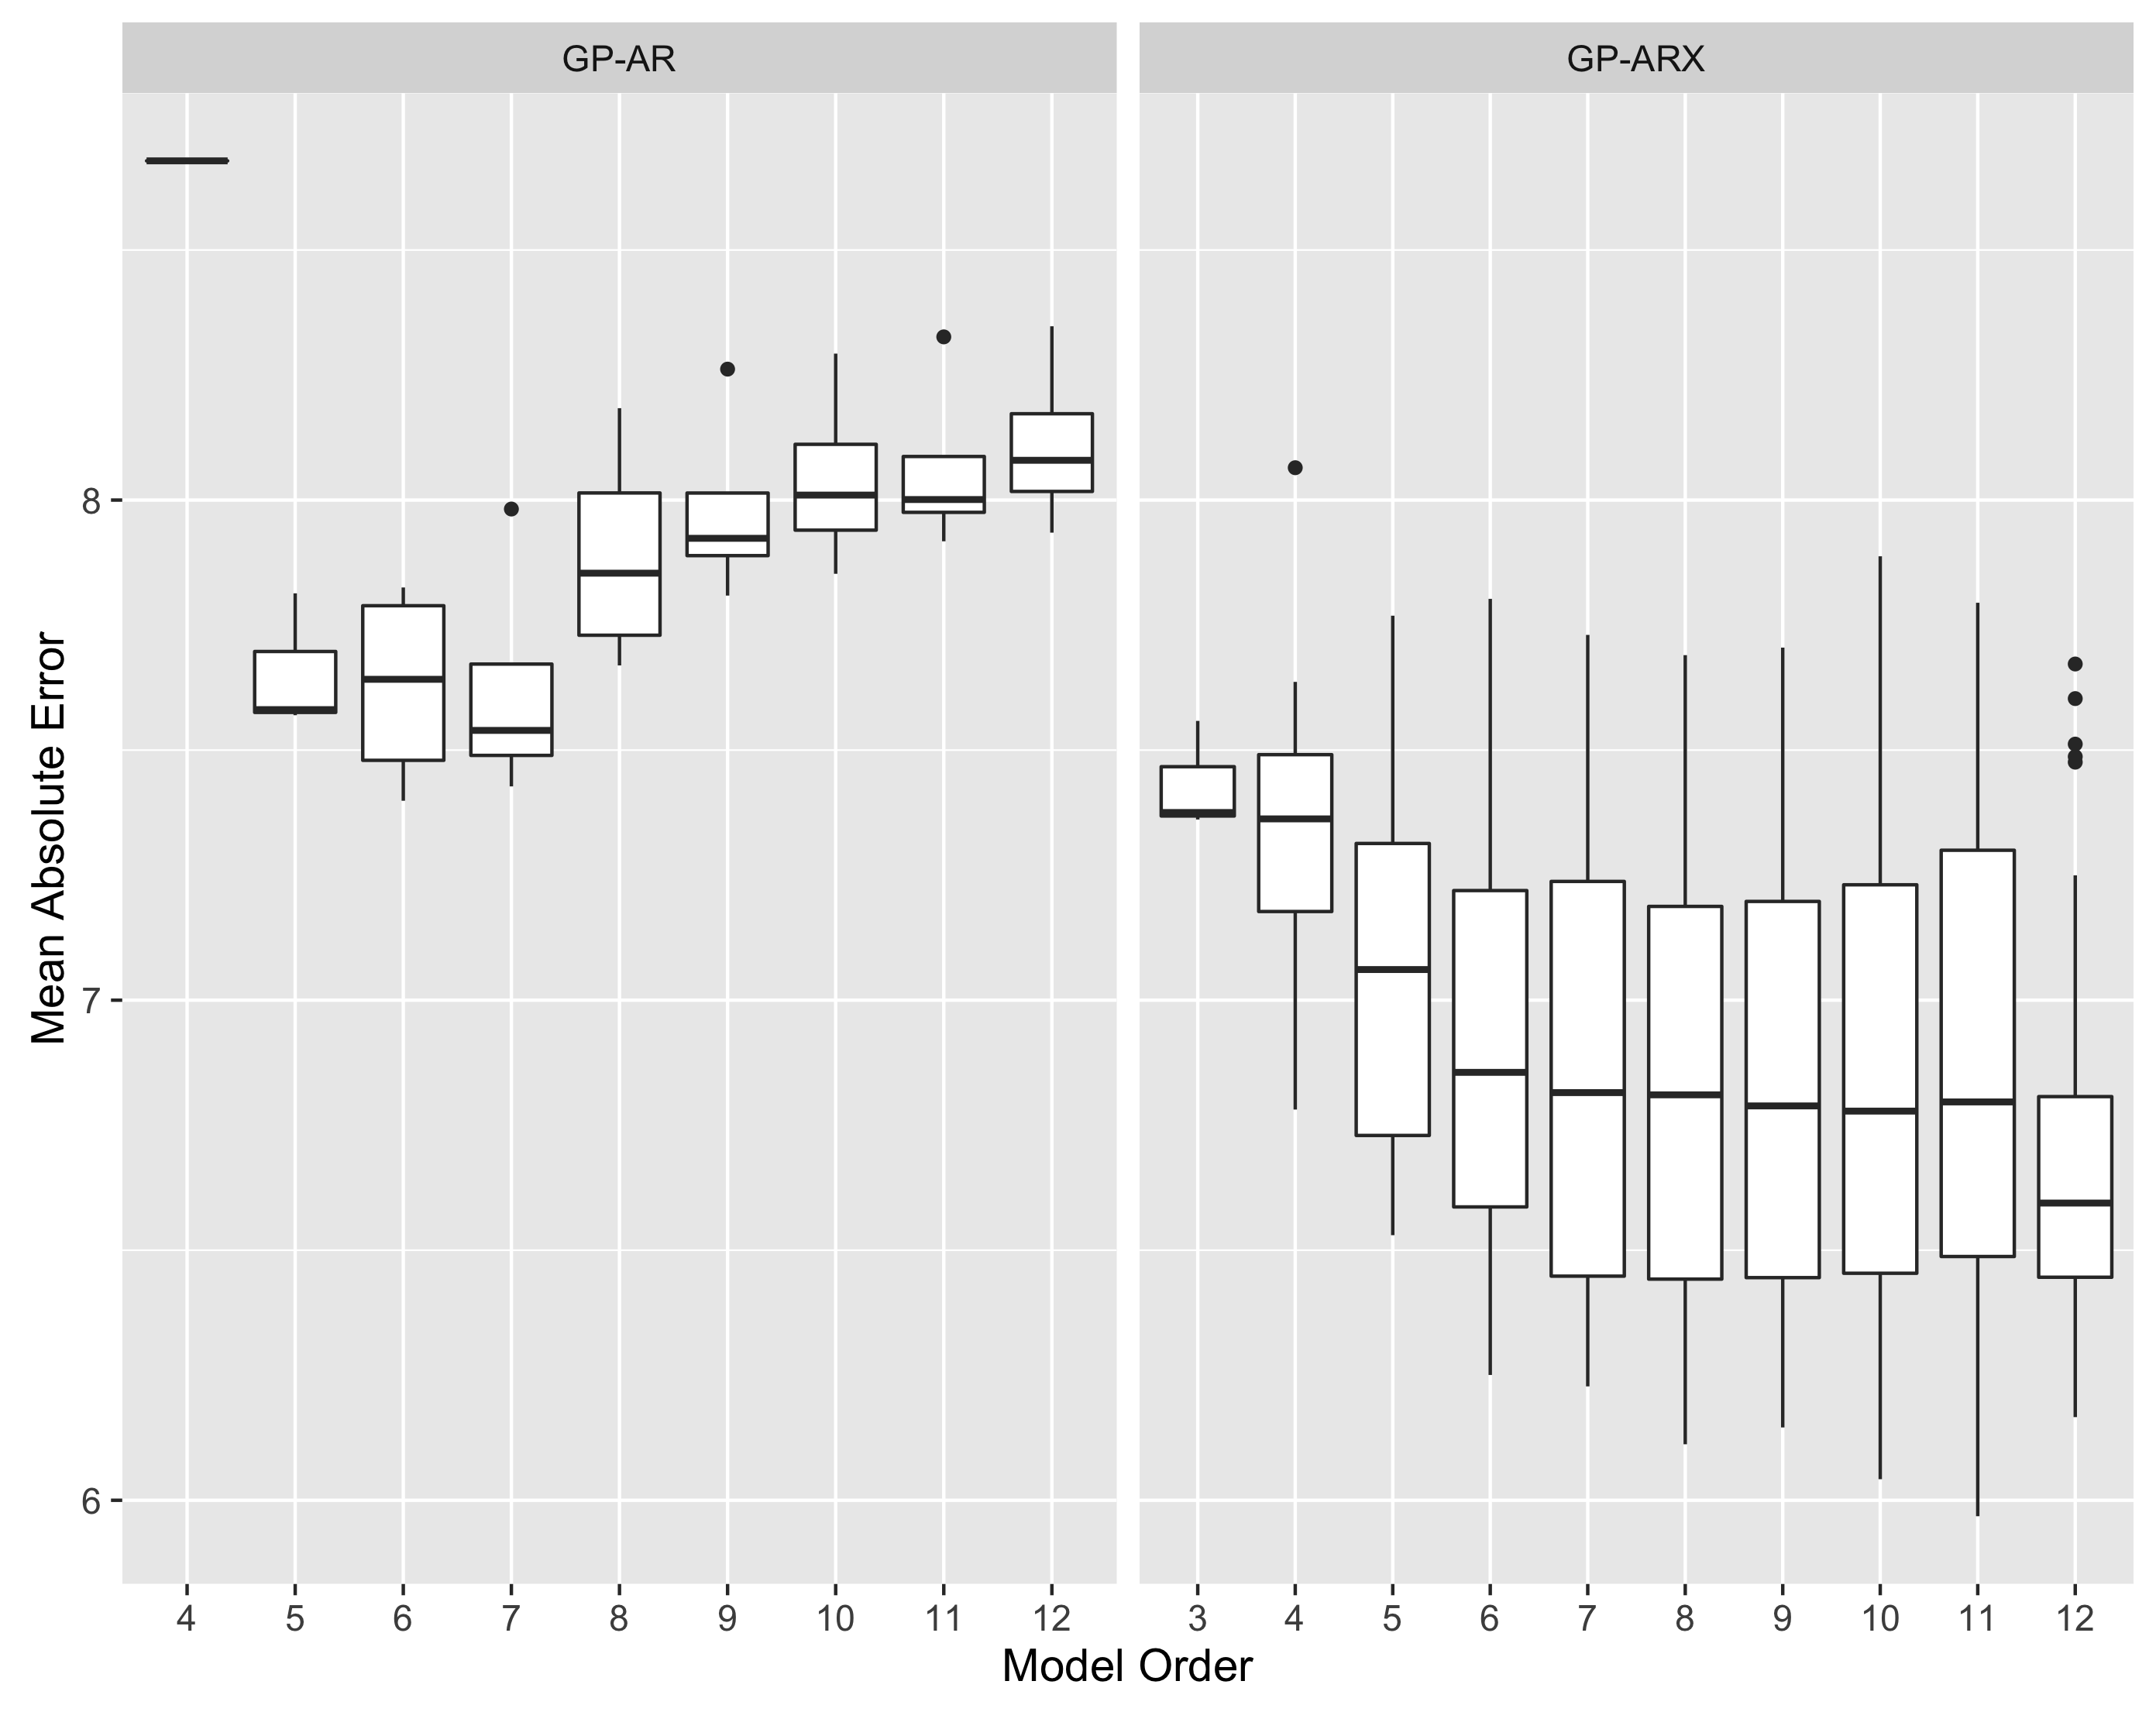
\includegraphics[width=\textwidth]{Compare-mae.png}
    \caption{Mean Absolute Error (\si{\nano\tesla}) on validation set storms vs model order for GP-AR and GP-ARX. \\ \textbf{Key}: Rectangle borders represent the first and third quartiles, with a horizontal line inside to indicate the median value, outlying points are shown as dots and whiskers indicate the smallest and largest non-outliers}
    \label{fig:CompareMae}
\end{figure}
    
\begin{figure}
    \noindent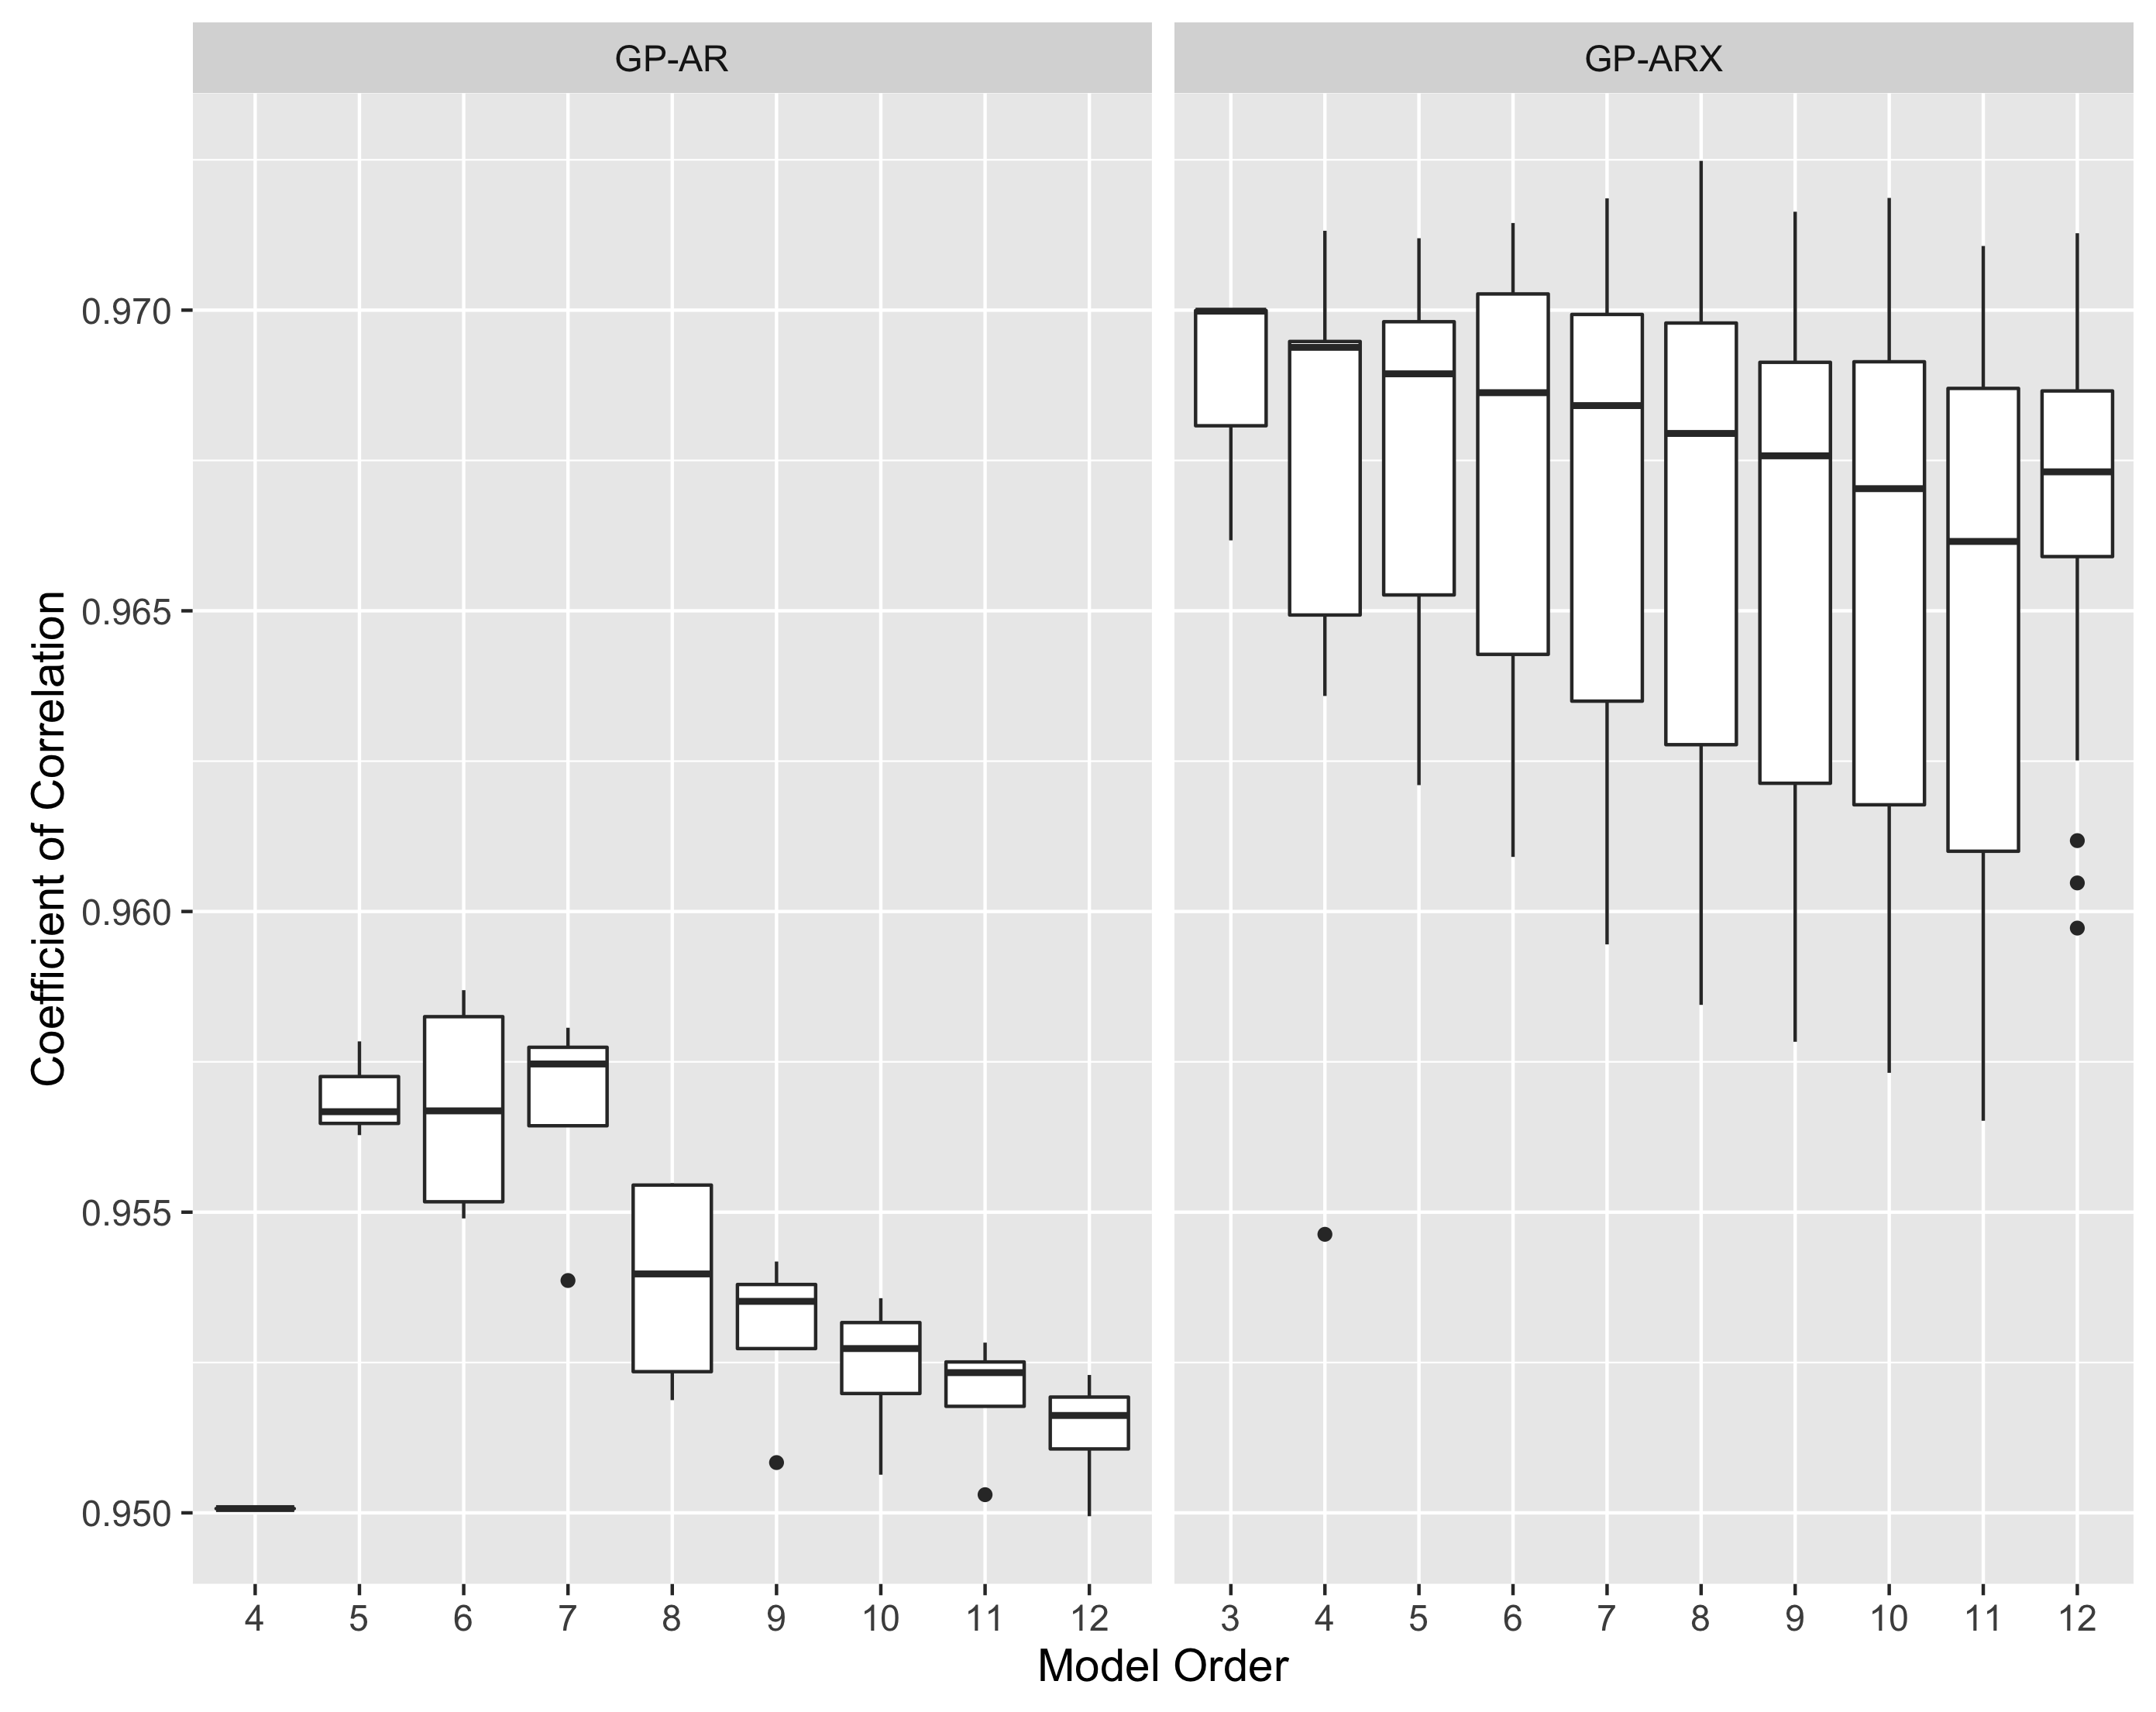
\includegraphics[width=\textwidth]{Compare-cc.png}
    \caption{Coefficient of Correlation on validation set storms vs model order for GP-AR and GP-ARX \\ \textbf{Key}: Rectangle borders represent the first and third quartiles, with a horizontal line inside to indicate the median value, outlying points are shown as dots and whiskers indicate the smallest and largest non-outliers}
    \label{fig:CompareCC}
\end{figure}
    
    
\begin{figure}
    \noindent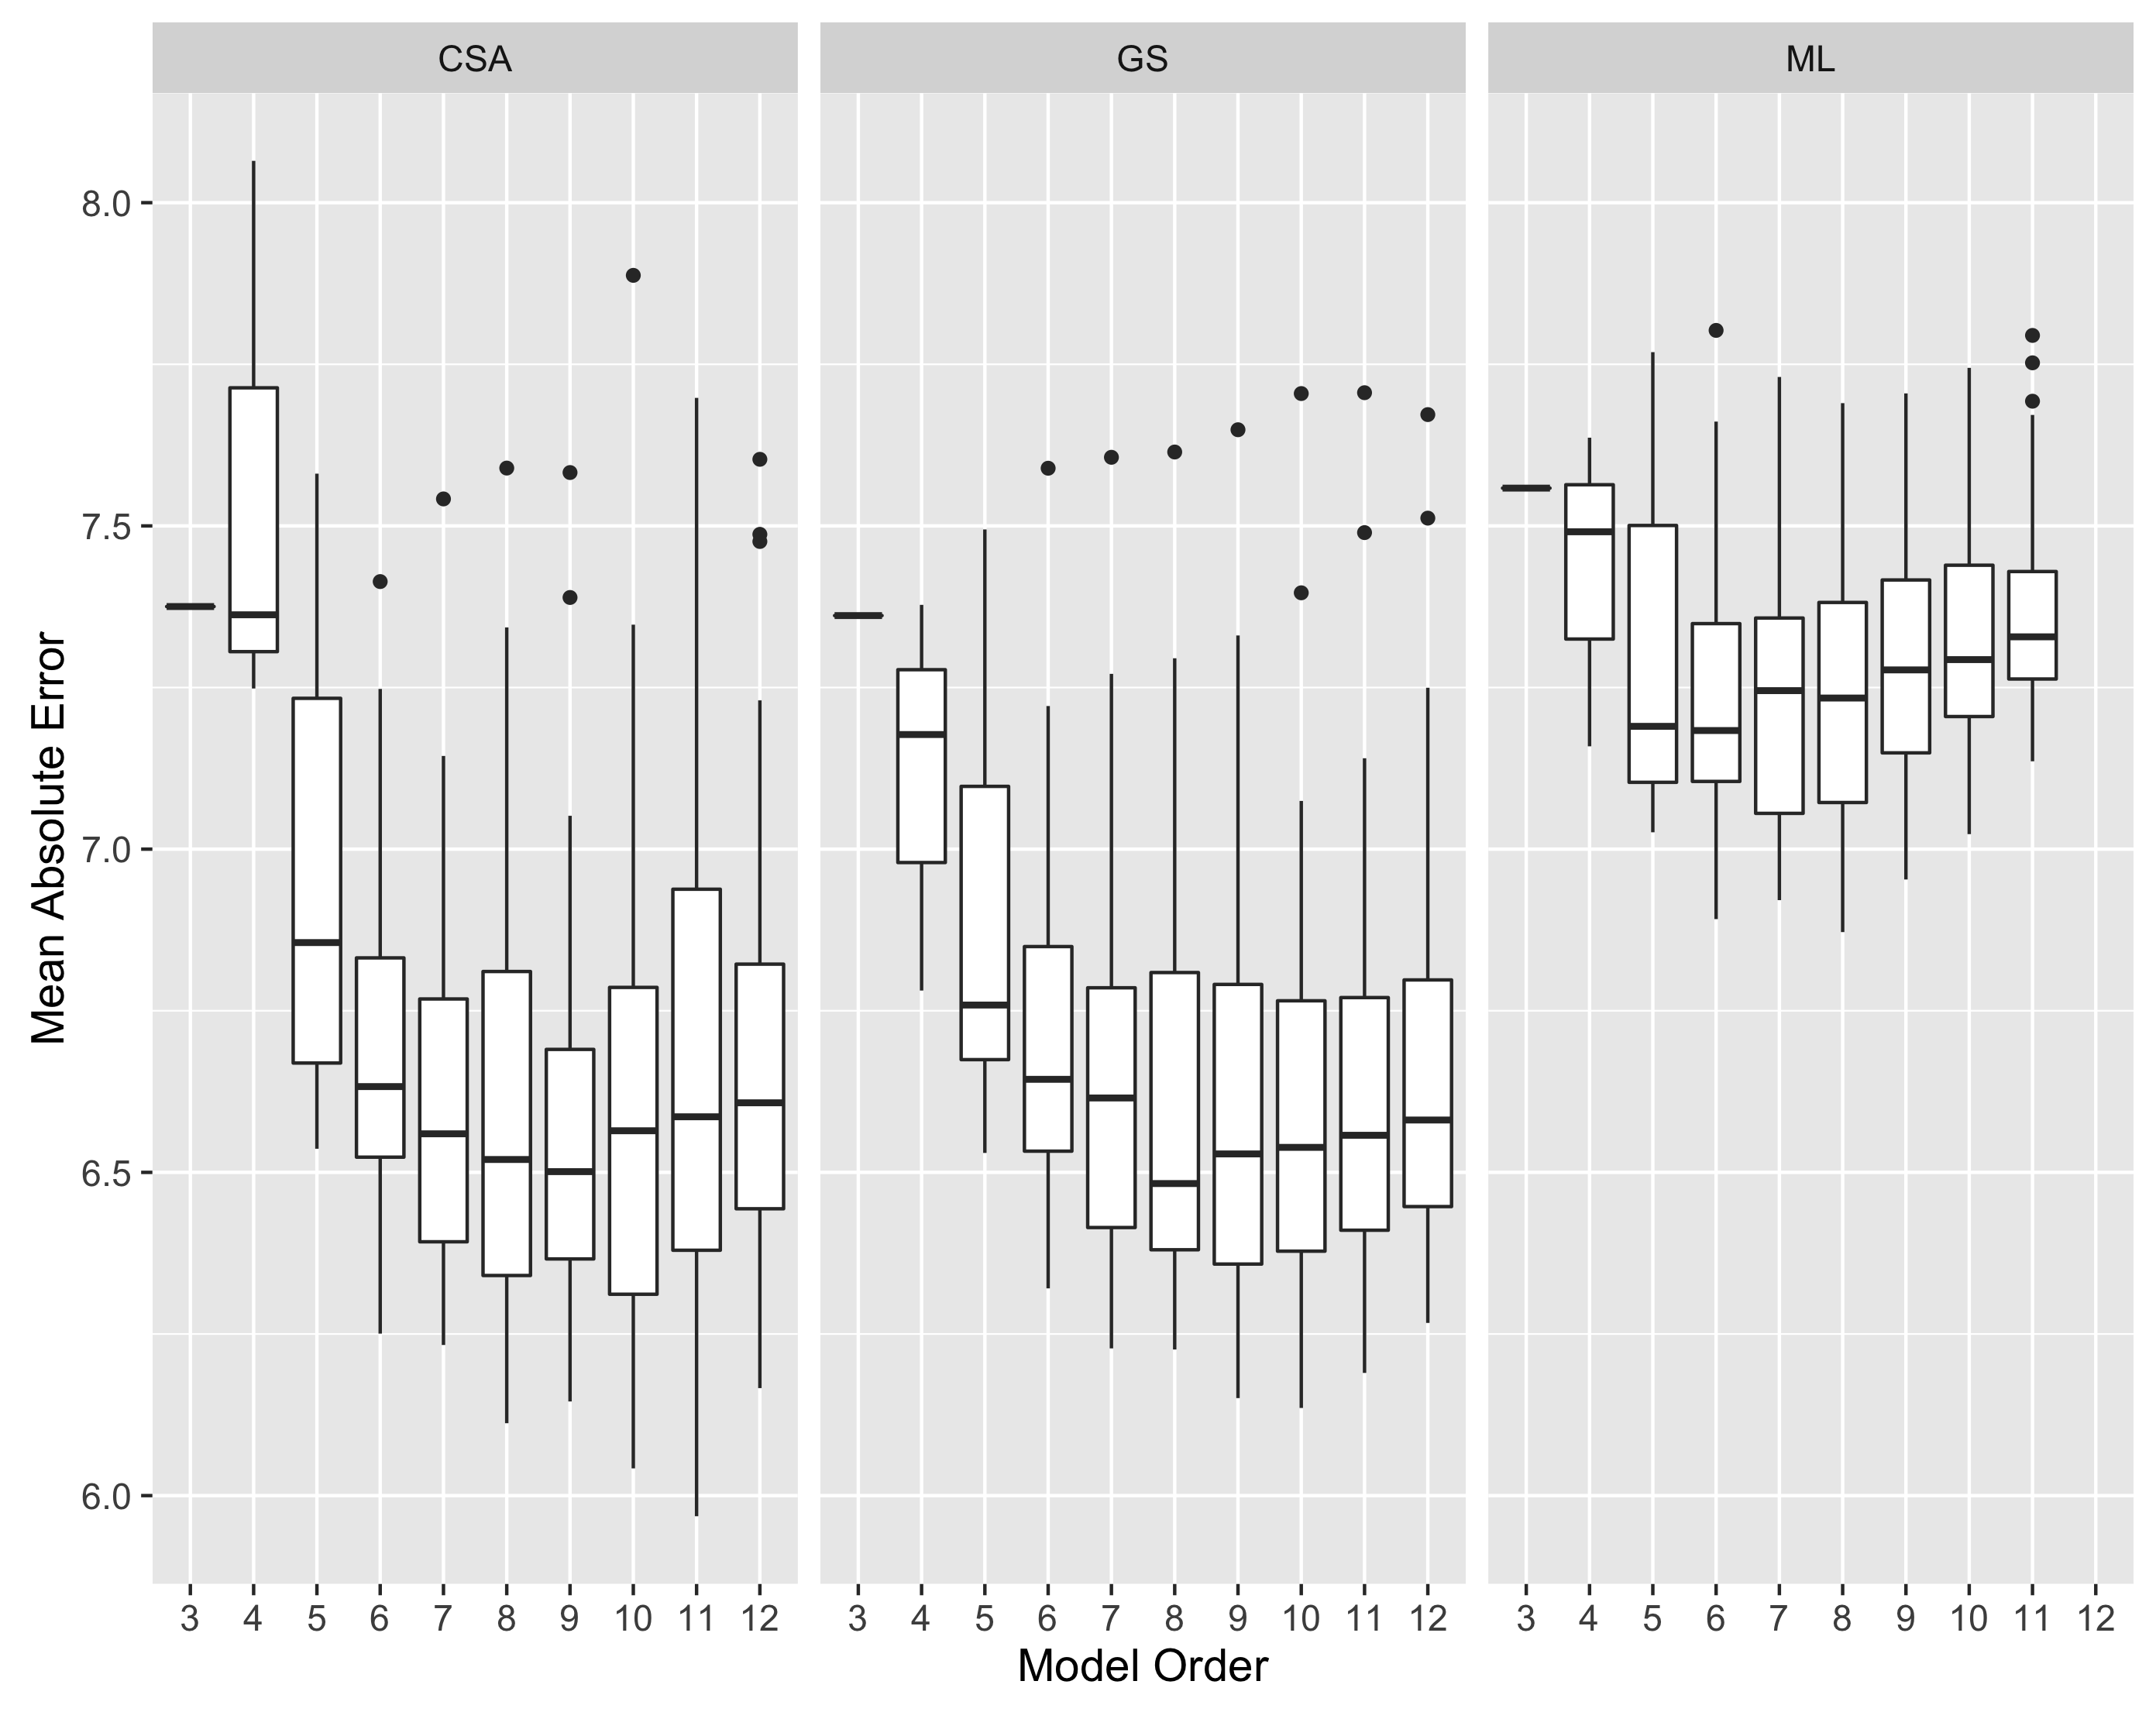
\includegraphics[width=\textwidth]{Compare-mae-arx.png}
    \caption{Mean Absolute Error (\si{\nano\tesla}) on validation set storms vs model order for GP-AR and GP-ARX for \emph{CSA}, \emph{GS} and \emph{ML} model selection routines \\ \textbf{Key}: Rectangle borders represent the first and third quartiles, with a horizontal line inside to indicate the median value, outlying points are shown as dots and whiskers indicate the smallest and largest non-outliers}
    \label{fig:CompareMaeARX}
\end{figure}
    
\begin{figure}
    \noindent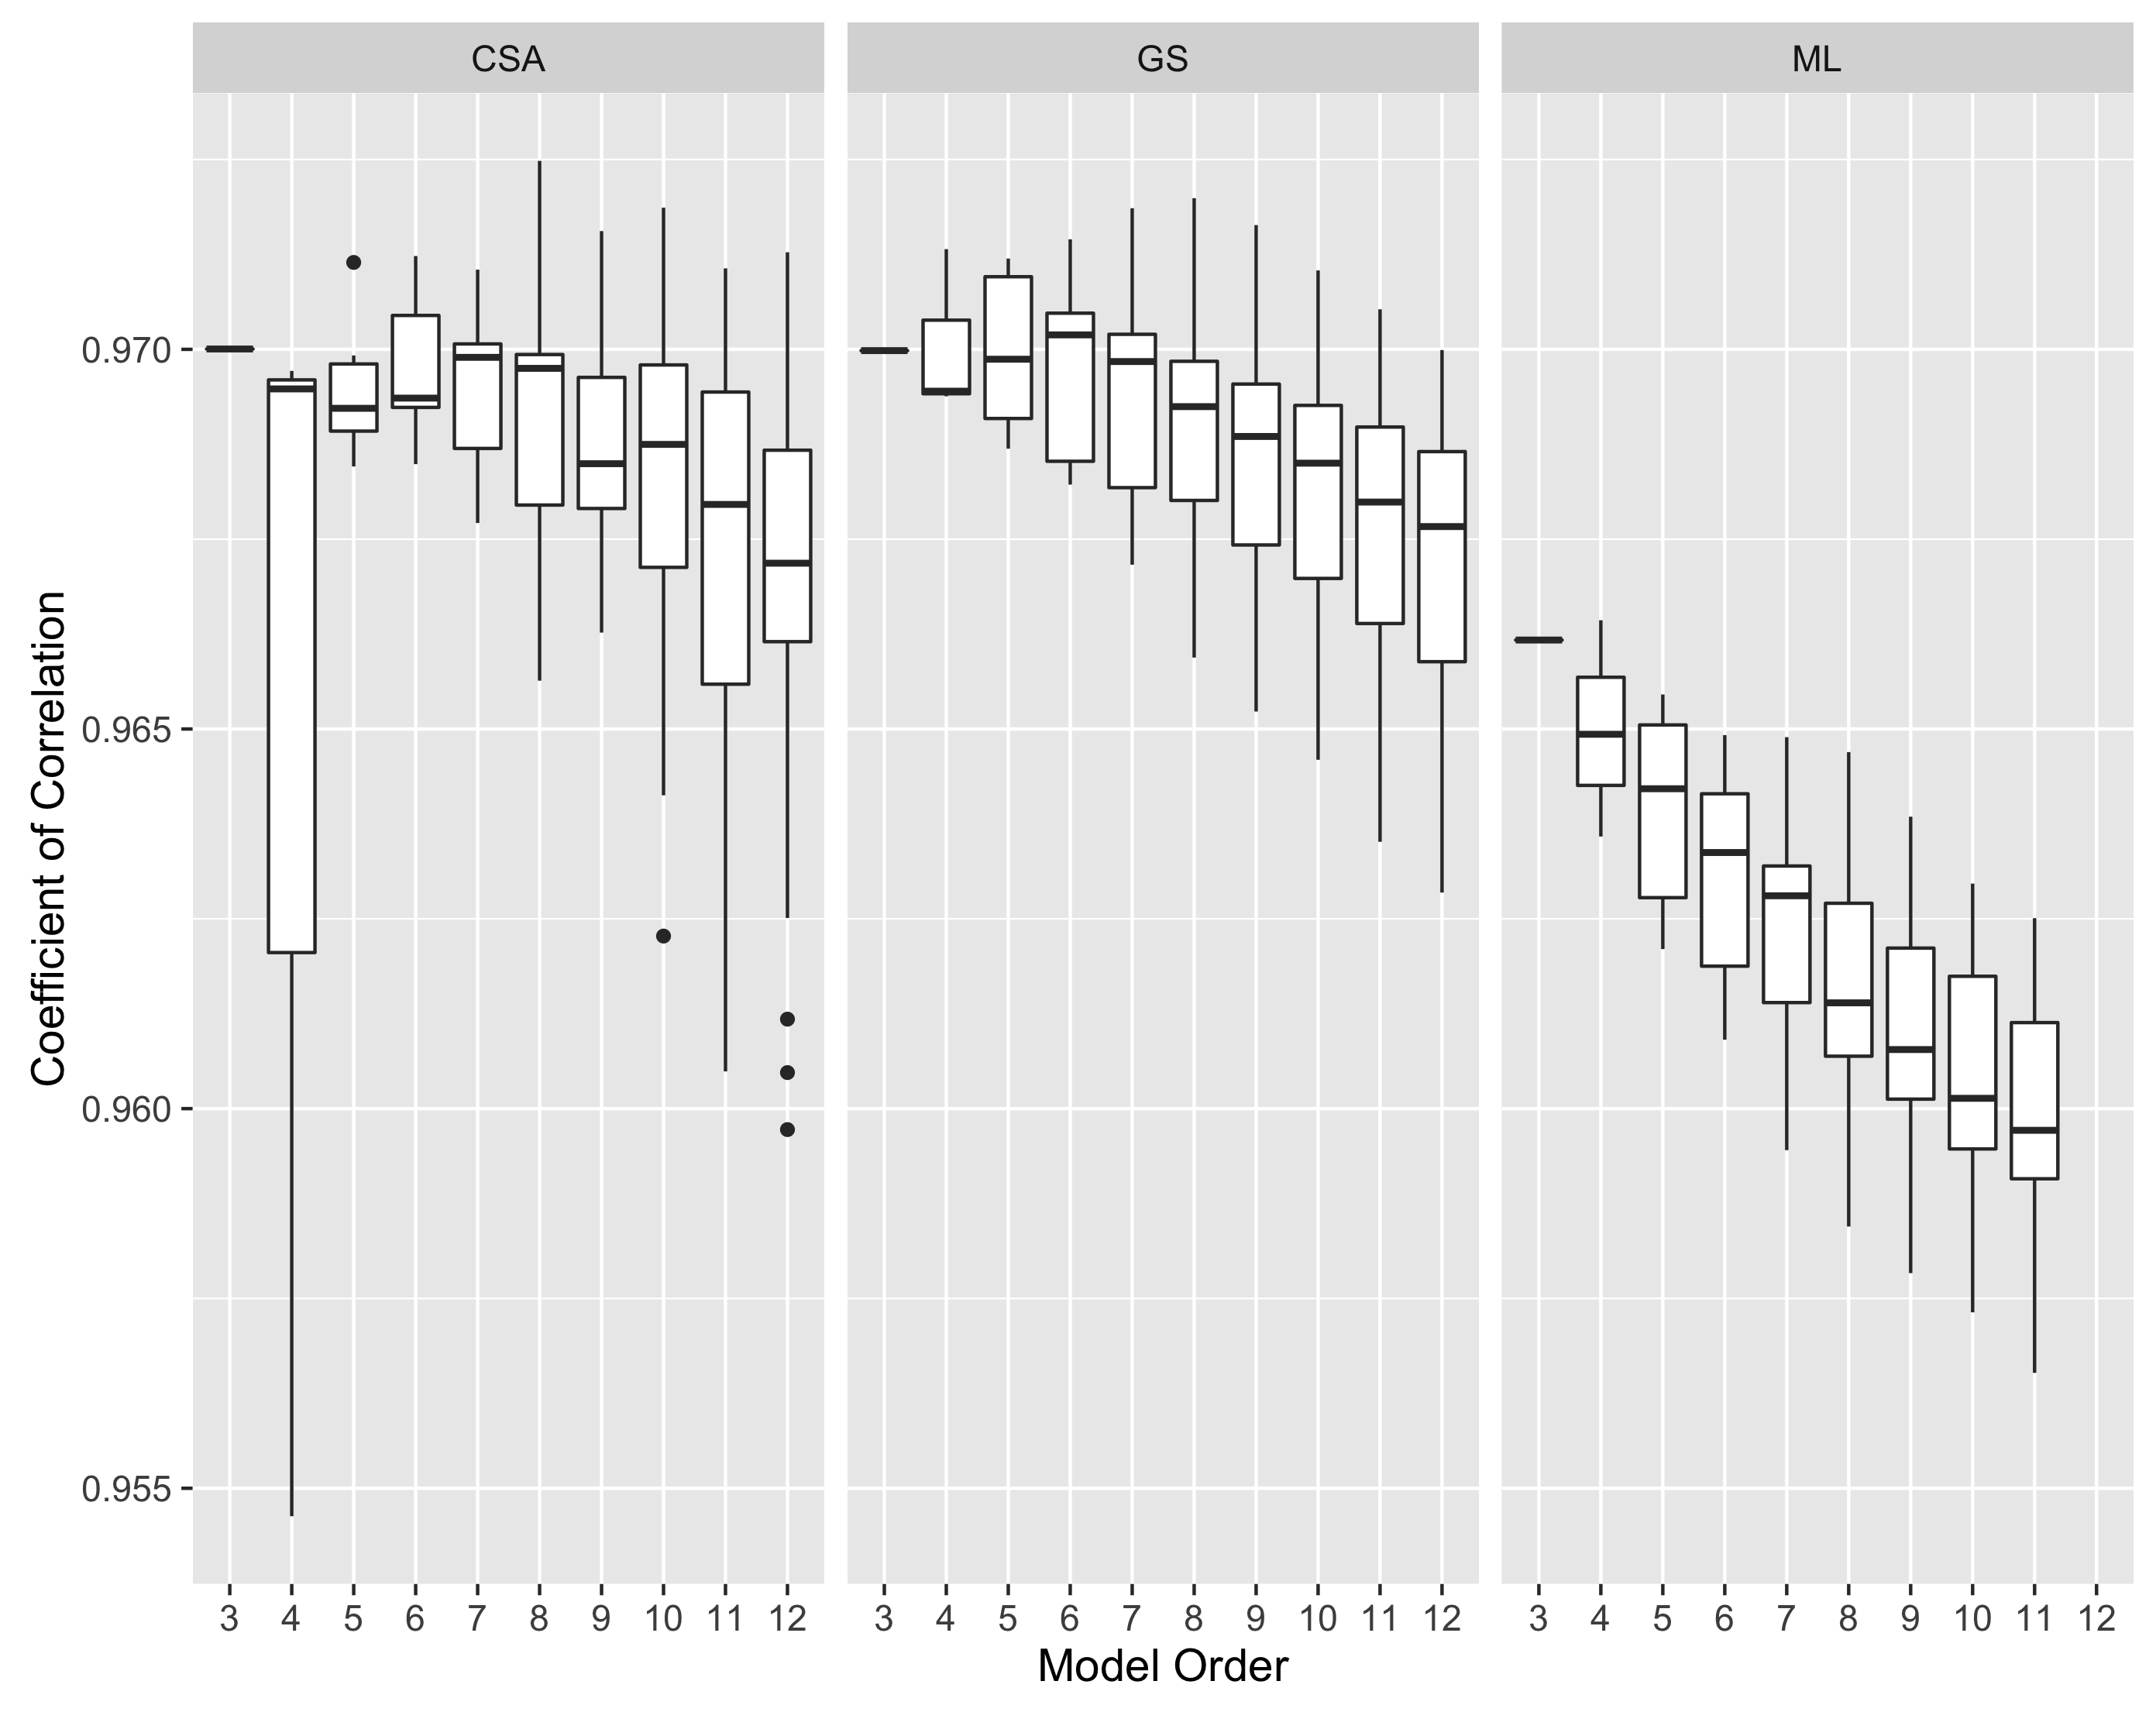
\includegraphics[width=\textwidth]{Compare-cc-arx.png}
    \caption{Coefficient of Correlation on validation set storms vs model order for GP-AR and GP-ARX for \emph{CSA}, \emph{GS} and \emph{ML} model selection routines \\ \textbf{Key}: Rectangle borders represent the first and third quartiles, with a horizontal line inside to indicate the median value, outlying points are shown as dots and whiskers indicate the smallest and largest non-outliers}
    \label{fig:CompareCCARX}
\end{figure}
    

Figures \ref{fig:CompareMae} and \ref{fig:CompareCC} show how the mean absolute error and coefficient of correlation as calculated on the validation set storm events of Table \ref{table:validationstorms}, vary with increasing model order for GP-AR and GP-ARX. The results are represented as box and whisker plots, in which a rectangle is drawn to represent the first and third quartiles, with a horizontal line inside to indicate the median value, outlying points are shown as dots while the whiskers indicate the smallest and largest non-outliers. In both cases, the predictive performance first improves and then stagnates or worsens with increasing model order. 

Figures \ref{fig:CompareMaeARX} and \ref{fig:CompareCCARX} break down the results for GP-ARX by the model selection routine used. Apart from the general trend observed in \ref{fig:CompareMae} and \ref{fig:CompareCC}, we also observe that \emph{grid search} and \emph{coupled simulated annealing} give superior performance as compared to gradient based \emph{maximum likelihood}.

From the validation results, we choose the model order which yields the best RMSE performance, for GP-AR it is $p_t = 6$ while for GP-ARX it is $p = 6, p_v = 1, p_b = 3$.

After choosing the best performing GP-AR and GP-ARX models, we calculate their performance on the test set of Table \ref{table:teststorms}. The results of these model evaluations are summarised in Table \ref{table:results}, the GP-AR and GP-ARX models improve upon the performance of the \emph{persistence model}.

Figures \ref{fig:ComparePred1}, \ref{fig:ComparePred2} and \ref{fig:ComparePred3} show OSA predictions of the GP-ARX model with $\pm \sigma$ error bars for three storm events in the time period between 1998 and 2003. The GP-ARX model gives accurate predictions along with plausible error bars around its mean predictions.

\section{Conclusions}

In this paper, we describe a flexible and expressive methodology for generating probabilistic forecasts of the $ \mathrm{Dst}$ index. We proposed two \emph{Gaussian Process} auto-regressive models, \emph{GP-ARX} and \emph{GP-AR}, to generate hourly predictions and their associated error bars. We also describe how to carry out model selection and validation of GP-AR and GP-ARX models.


Our results can be summarised as follows.
\begin{enumerate}
      \item \emph{Persistence} model plays an important role in the model building and evaluation process in the context of \emph{one step ahead} prediction of the $ \mathrm{Dst}$ index. Although it is not a robust predictor for the onset of intense geomagnetic storms, the \emph{persistence model} performs well on classical error metrics such as \emph{root mean square error} and such. From the considerations above, it is quite evident that classical performance metrics are not adequate for model evaluation, nevertheless in space weather literature, metrics such as \emph{RMSE} are very commonly used to compare predictive performance of models. Although not the research focus of this study, we note that there exists a need for the formulation of more informative performance metrics for measurement of predictive performance of geomagnetic predictive models.
      
      \item \emph{Gaussian Process} AR and ARX models give encouraging benefits in OSA prediction. Leveraging the strengths of the Bayesian approach, they are able to learn robust predictors from data. If one considers the size of the data used in our study, one can appreciate that the models presented here need relatively small training and validations sets: the training set contains 243 instances, while the validation set contains 782 instances.
      
      \item Since the GP models generate predictive distributions for test data and not just point predictions they lend themselves to the requirements of space weather prediction very well because of the need to generate error bars on predictions.
      
      \item The \emph{Gaussian Process} regression framework described in this study can also be extended to multiple hour ahead prediction of $ \mathrm{Dst}$, which is currently a work in progress.
\end{enumerate}




%%% End of body of article:

%%%%%%%%%%%%%%%%%%%%%%%%%%%%%%%%
%% Optional Appendix goes here
%
% \appendix resets counters and redefines section heads
% but doesn't print anything.
% After typing \appendix
%
%\section{Here Is Appendix Title}
% will show
% Appendix A: Here Is Appendix Title
%
%%%%%%%%%%%%%%%%%%%%%%%%%%%%%%%%%%%%%%%%%%%%%%%%%%%%%%%%%%%%%%%%
%
% Optional Glossary or Notation section, goes here
%

%%%%%%%%%%%%%%
% Notation -- End each entry with a period.
% \begin{notation}
% Term & definition.\\
% Second term & second definition.\\
% \end{notation}
%%%%%%%%%%%%%%%%%%%%%%%%%%%%%%%%%%%%%%%%%%%%%%%%%%%%%%%%%%%%%%%%
%
%  ACKNOWLEDGMENTS

%\begin{acknowledgments}
%We acknowledge use of NASA/GSFC's Space Physics Data Facility's OMNIWeb (or CDAWeb or ftp) service, and OMNI data. Simon Wing acknowledges supports from CWI and NSF Grant AGS-1058456 and NASA Grants (NNX13AE12G, NNX15AJ01G, NNX16AC39G).
%\end{acknowledgments}


    
\begin{figure}
    \noindent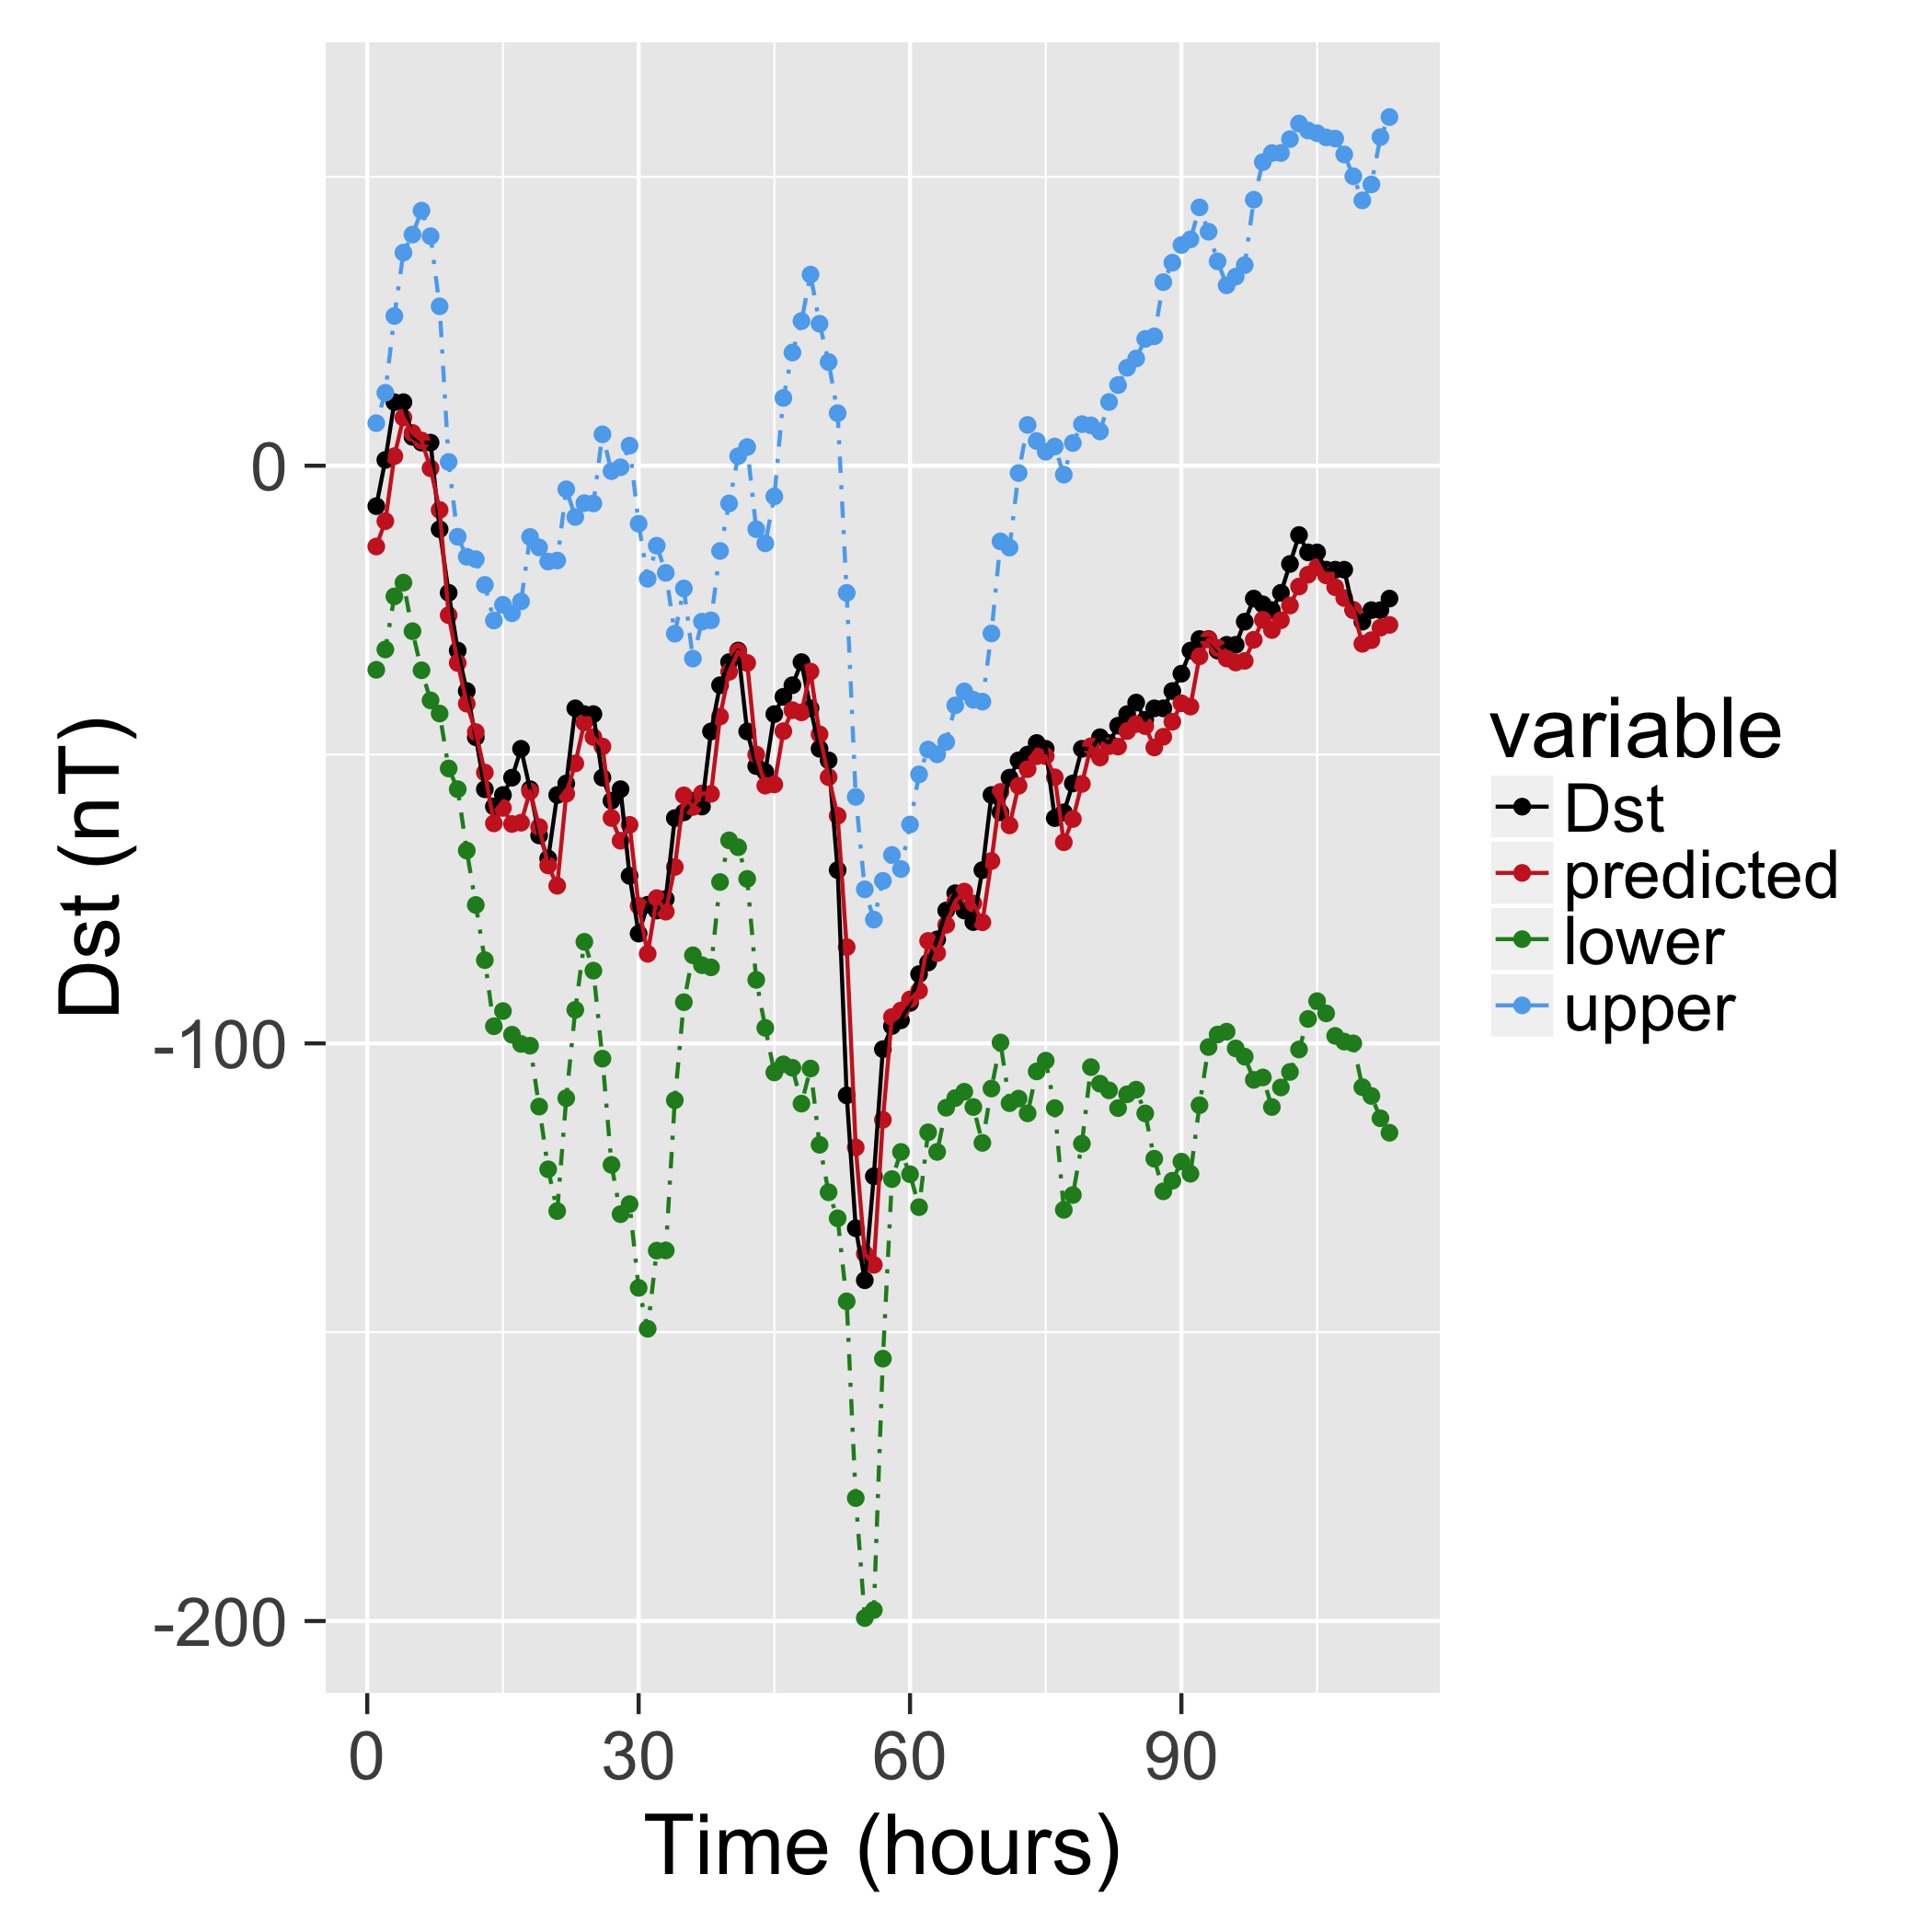
\includegraphics[width=\textwidth]{PredictionsModel1/PredErrBars_Storm43.png}
    \caption{OSA Predictions with $\pm \sigma$ error bars for event: 2003/06/17 to 2003/06/19}
    \label{fig:ComparePred1}
\end{figure}
    
    
\begin{figure}
    \noindent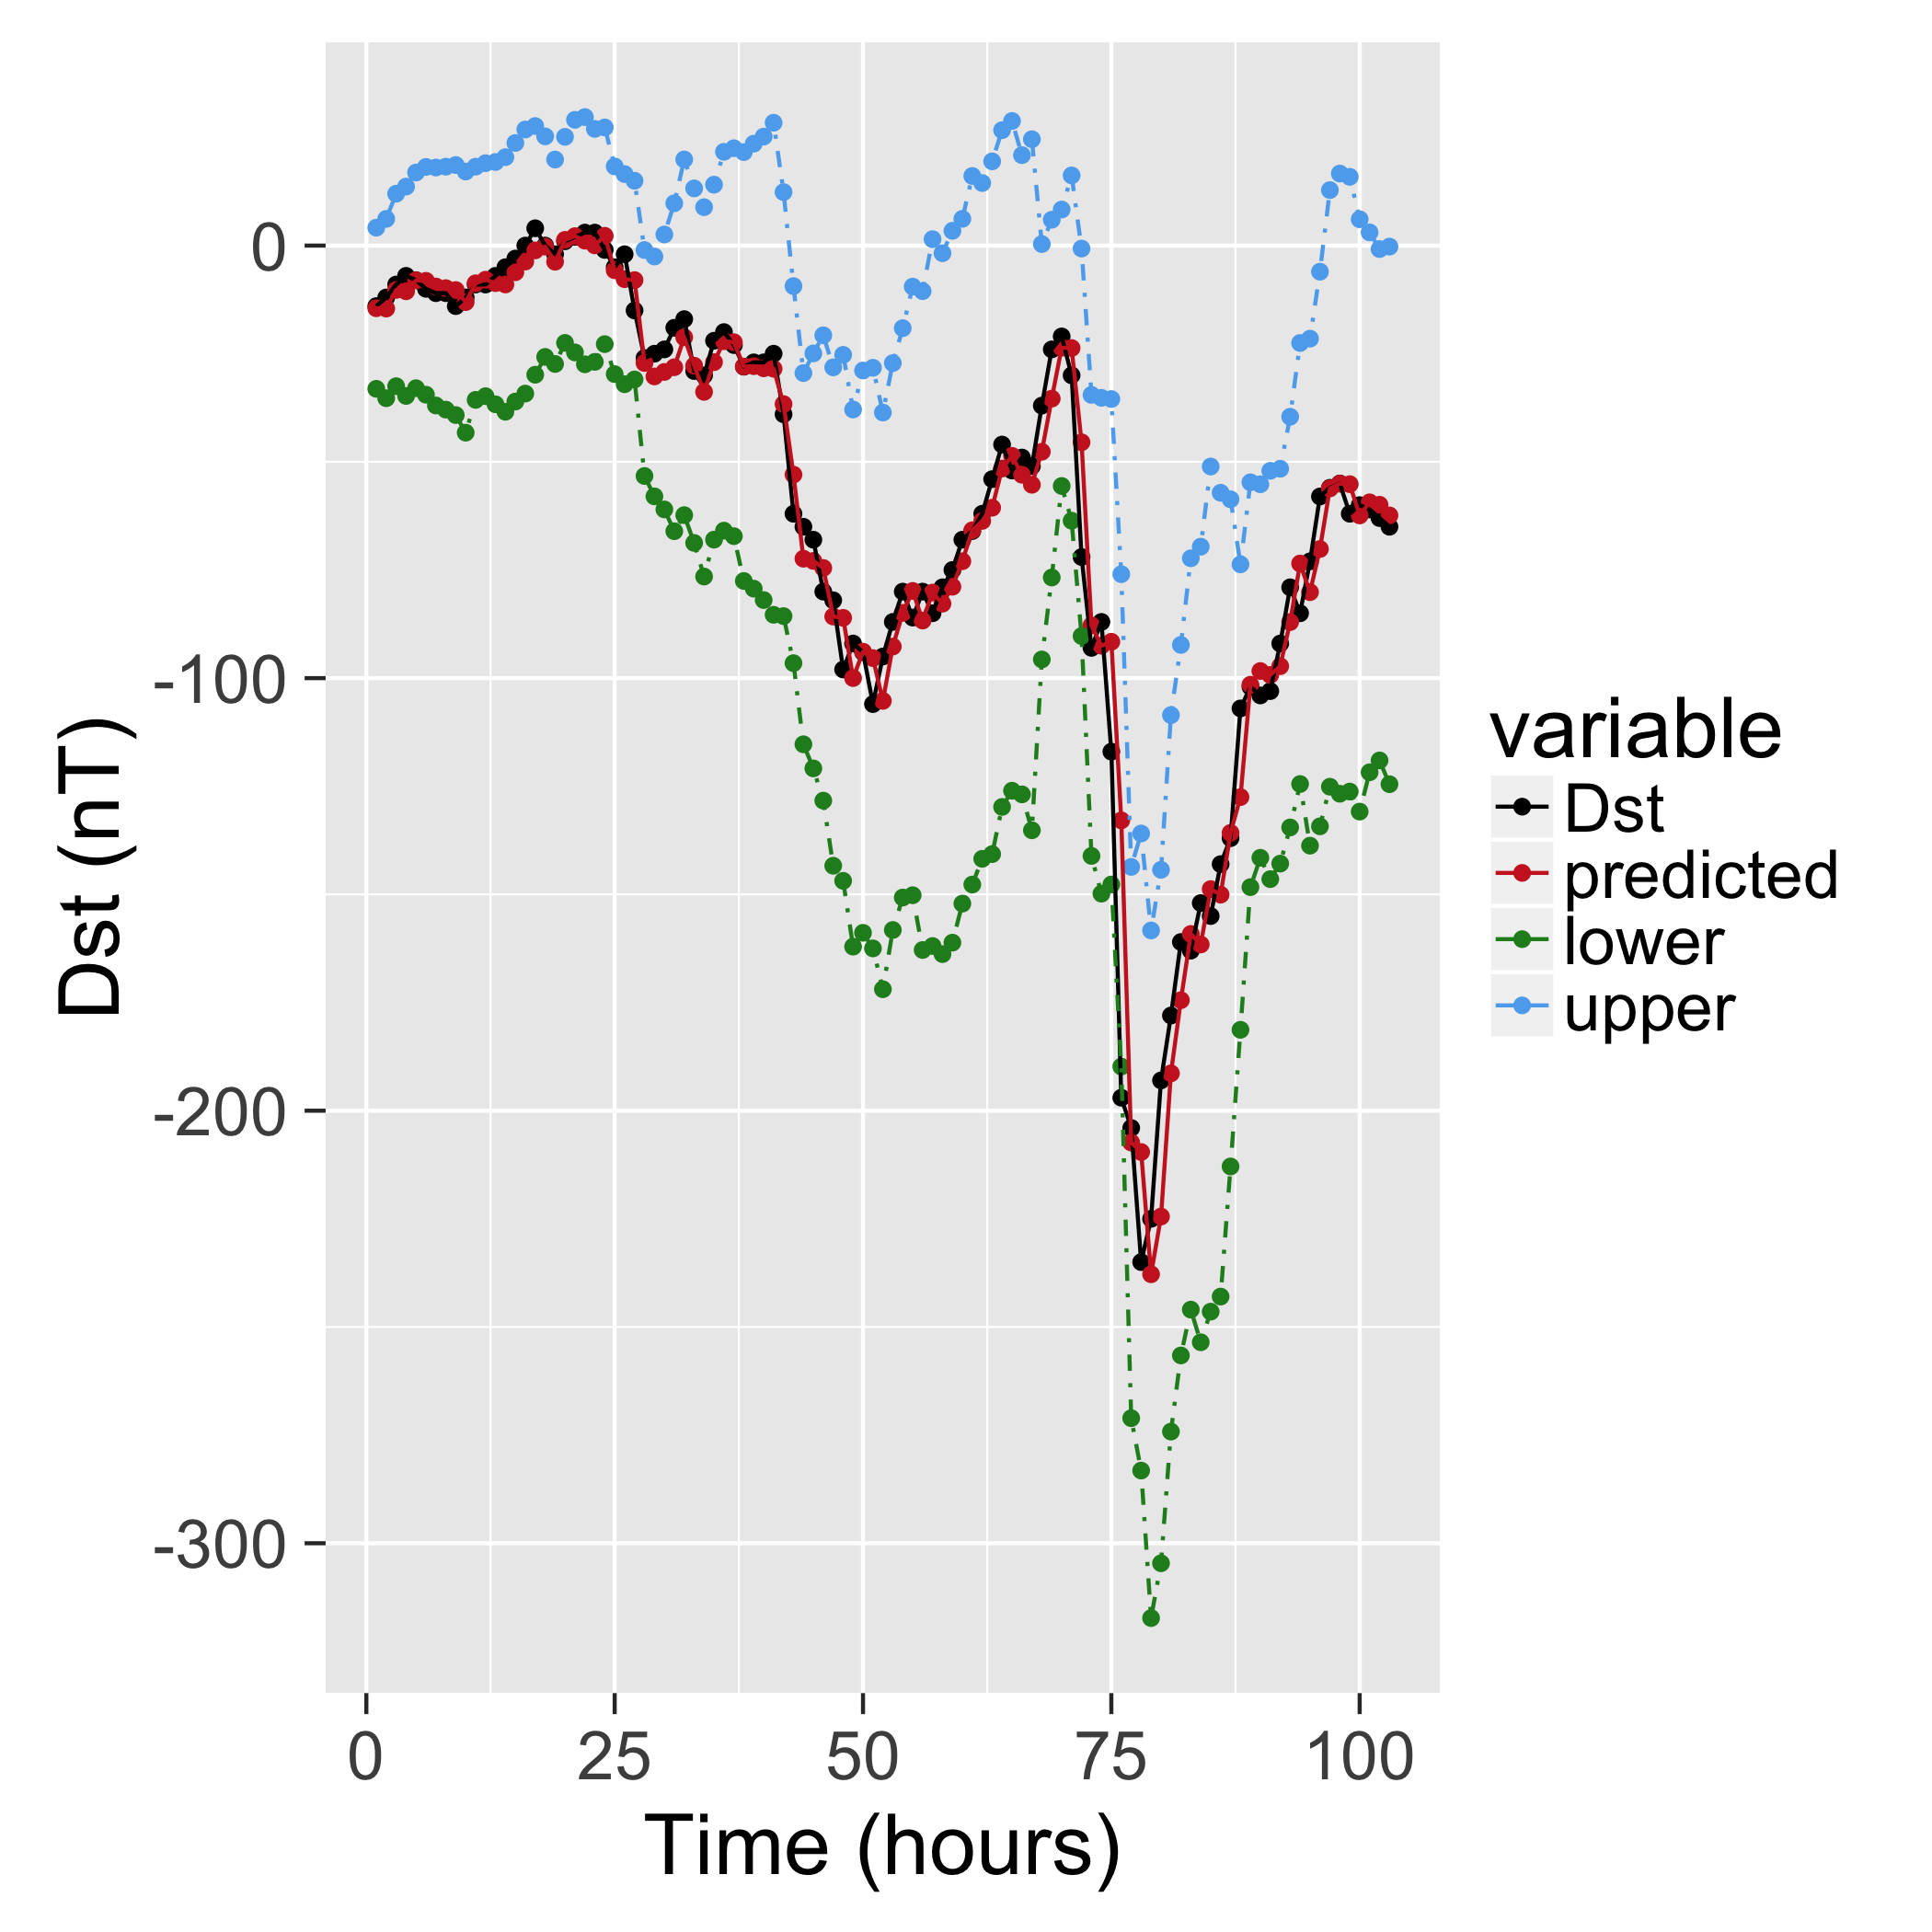
\includegraphics[width=\textwidth]{PredictionsModel1/PredErrBars_Storm16.png}
    \caption{OSA Predictions with $\pm \sigma$ error bars for event: 2012/03/08 to 2012/03/10}
    \label{fig:ComparePred2}
\end{figure}
    
\begin{figure}
    \noindent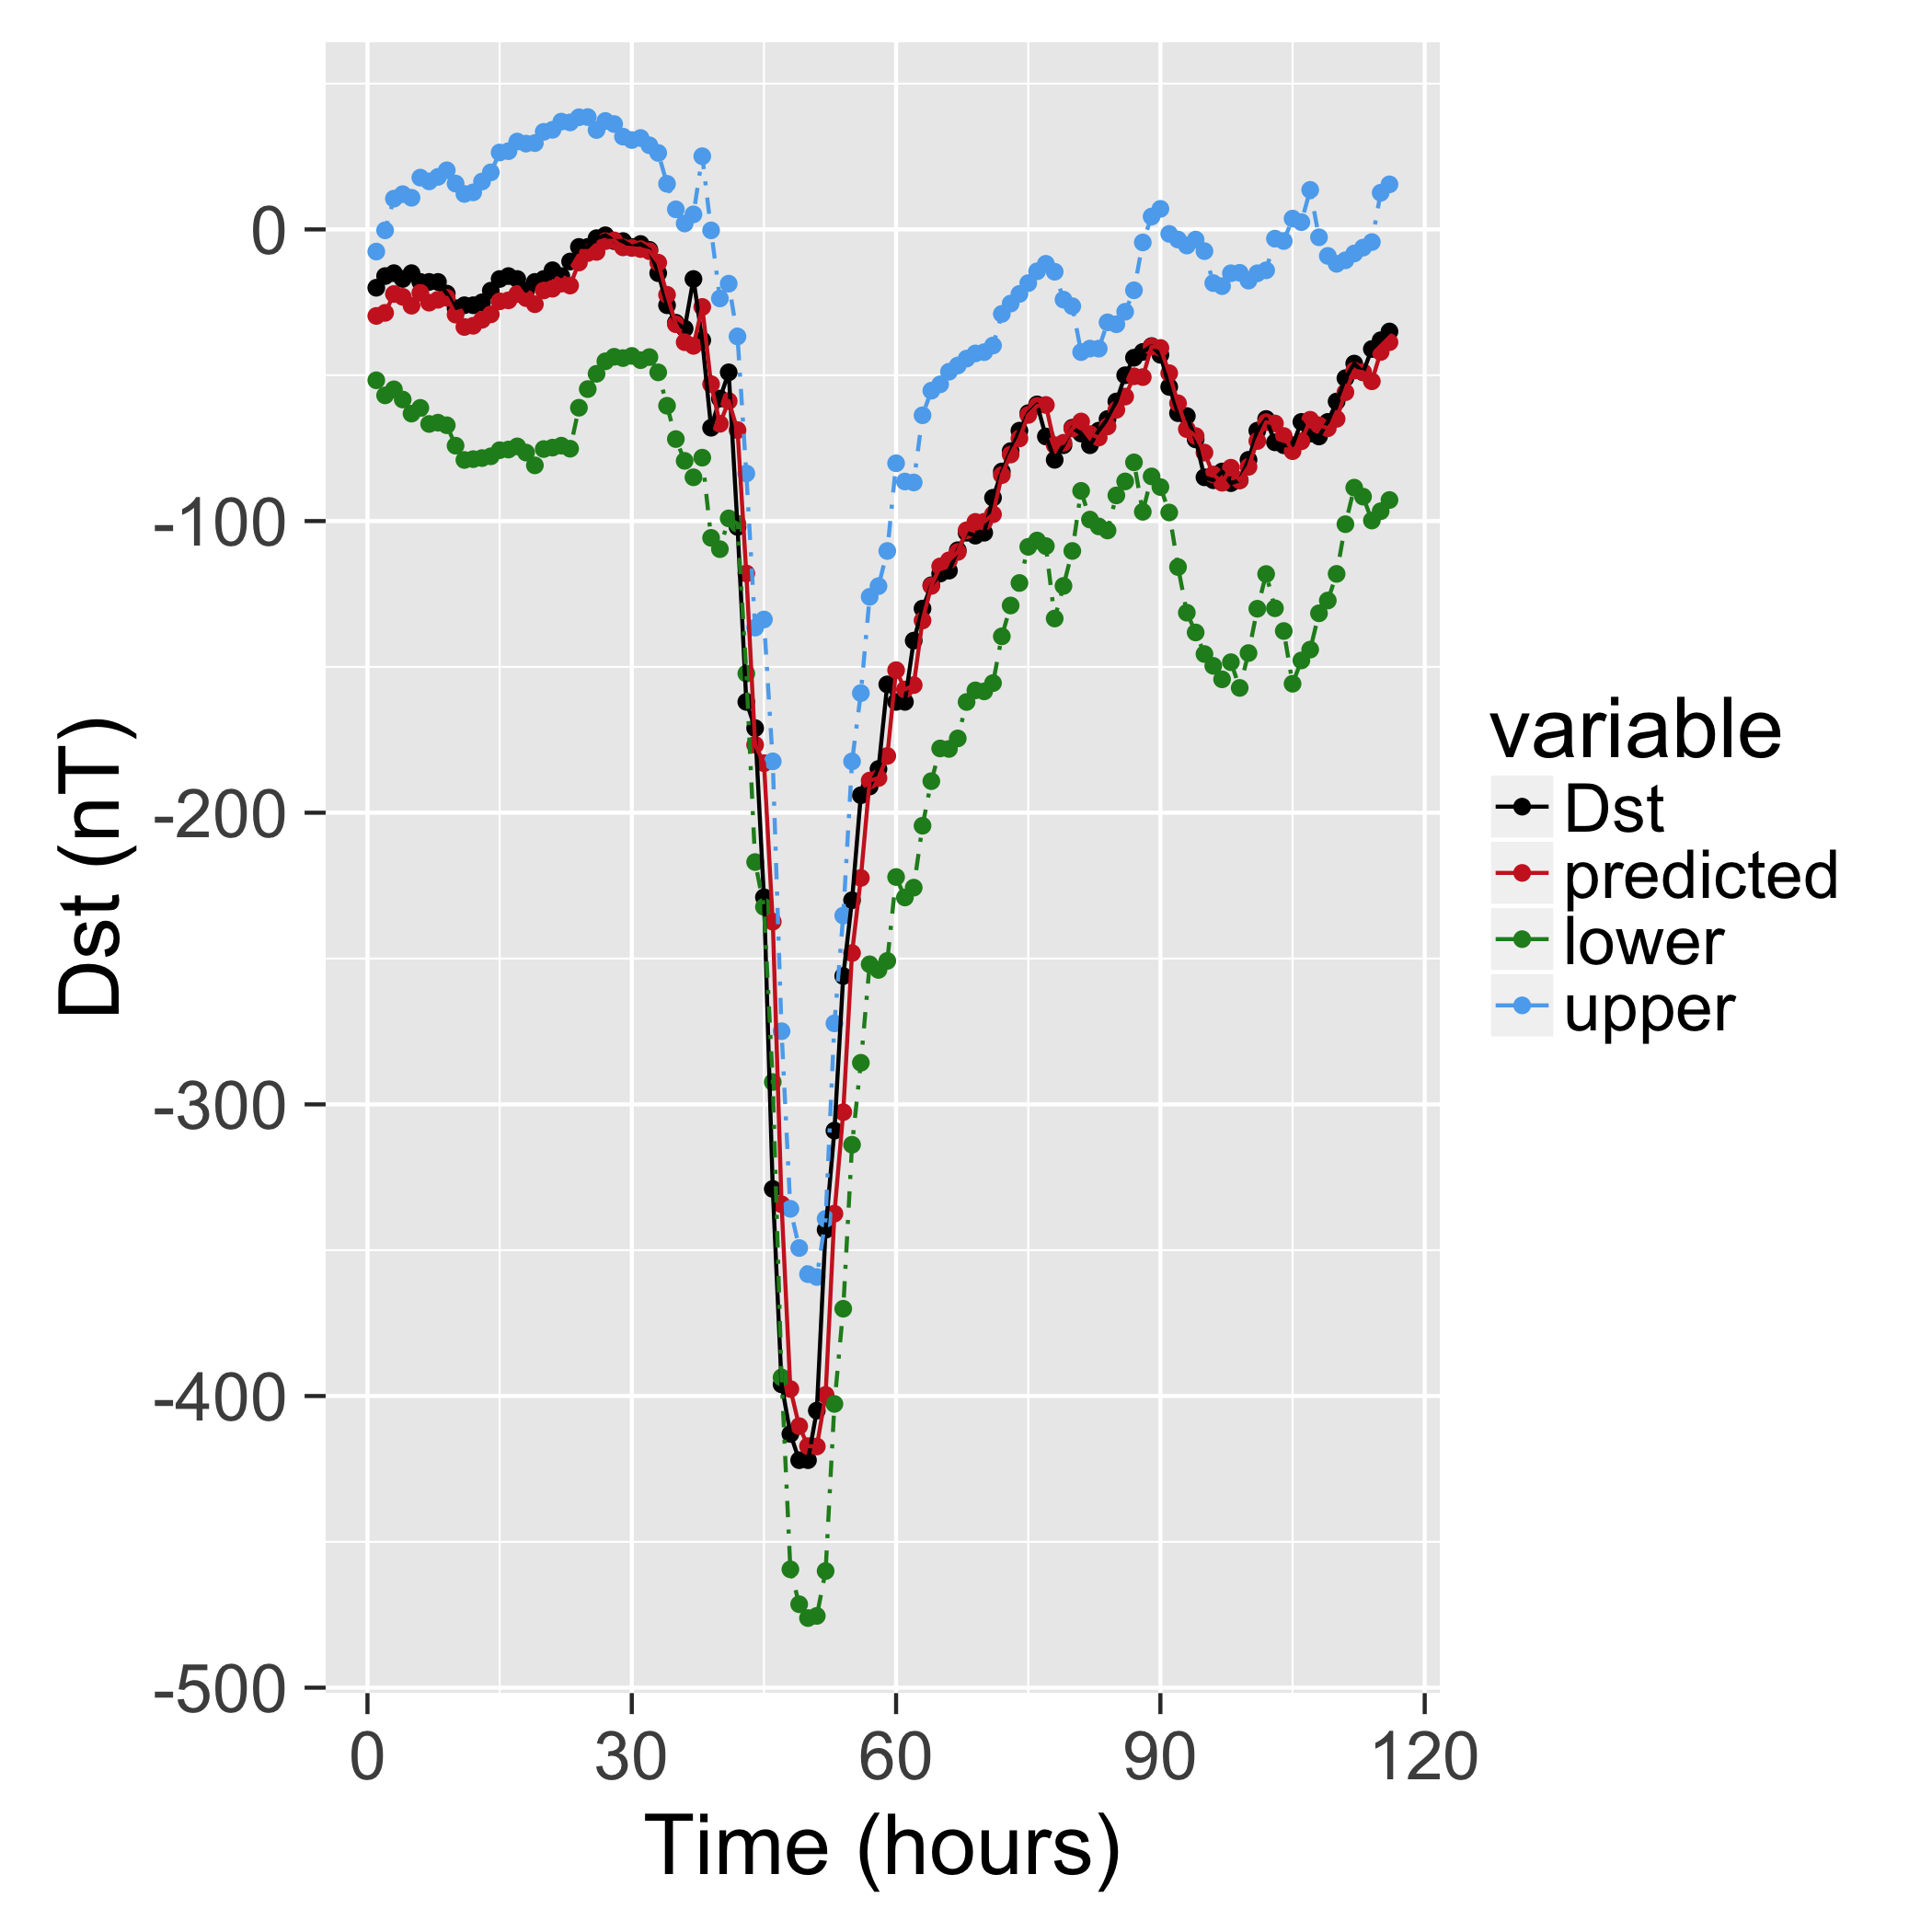
\includegraphics[width=\textwidth]{PredictionsModel1/PredErrBars_Storm46.png}
    \caption{OSA Predictions with $\pm \sigma$ error bars for event: 2003/11/20 to 2003/11/22}
    \label{fig:ComparePred3}
\end{figure}
    
    
    
    
    
    
\begin{table}[ht]
    \centering
    \caption{Storm events used for model selection of GP-AR and GP-ARX}
    \label{table:validationstorms}
    \begin{tabular}{llllll}
    \hline
    \textbf{Event Id} & \textbf{Start Date} & \textbf{Start Hour} & \textbf{End Date} & \textbf{End Hour} & \textbf{Storm Peak} \\ \hline
    1 & 1995/03/26 & 05:00 & 1995/03/26 & 23:00 & $ \SI{-107}{\nano\tesla}$ \\
    2 & 1995/04/07 & 13:00 & 1995/04/09 & 09:00 & $ \SI{-149}{\nano\tesla}$ \\
    3 & 1995/09/27 & 01:00 & 1995/09/28 & 04:00 & $ \SI{-108}{\nano\tesla}$ \\
    4 & 1995/10/18 & 13:00 & 1995/10/19 & 14:00 & $ \SI{-127}{\nano\tesla}$ \\
    5 & 1996/10/22 & 22:00 & 1996/10/23 & 11:00 & $ \SI{-105}{\nano\tesla}$ \\
    6 & 1997/04/21 & 10:00 & 1997/04/22 & 09:00 & $ \SI{-107}{\nano\tesla}$ \\
    7 & 1997/05/15 & 03:00 & 1997/05/16 & 00:00 & $ \SI{-115}{\nano\tesla}$ \\
    8 & 1997/10/10 & 18:00 & 1997/10/11 & 19:00 & $ \SI{-130}{\nano\tesla}$ \\
    9 & 1997/11/07 & 00:00 & 1997/11/07 & 18:00 & $ \SI{-110}{\nano\tesla}$ \\
    10 & 1997/11/22 & 21:00 & 1997/11/24 & 04:00 & $ \SI{-108}{\nano\tesla}$ \\
    11 & 2005/06/12 & 17:00 & 2005/06/13 & 19:00 & $ \SI{-106}{\nano\tesla}$ \\
    12 & 2005/08/31 & 12:00 & 2005/09/01 & 12:00 & $ \SI{-122}{\nano\tesla}$ \\
    13 & 2006/12/14 & 21:00 & 2006/12/16 & 03:00 & $ \SI{-162}{\nano\tesla}$ \\
    14 & 2011/09/26 & 14:00 & 2011/09/27 & 12:00 & $ \SI{-101}{\nano\tesla}$ \\
    15 & 2011/10/24 & 20:00 & 2011/10/25 & 14:00 & $ \SI{-132}{\nano\tesla}$ \\
    16 & 2012/03/08 & 12:00 & 2012/03/10 & 16:00 & $ \SI{-131}{\nano\tesla}$ \\
    17 & 2012/04/23 & 11:00 & 2012/04/24 & 13:00 & $ \SI{-108}{\nano\tesla}$ \\
    18 & 2012/07/15 & 01:00 & 2012/07/16 & 23:00 & $ \SI{-127}{\nano\tesla}$ \\
    19 & 2012/09/30 & 13:00 & 2012/10/01 & 18:00 & $ \SI{-119}{\nano\tesla}$ \\
    20 & 2012/10/08 & 02:00 & 2012/10/09 & 17:00 & $ \SI{-105}{\nano\tesla}$ \\
    21 & 2012/11/13 & 18:00 & 2012/11/14 & 18:00 & $ \SI{-108}{\nano\tesla}$ \\
    22 & 2013/03/17 & 07:00 & 2013/03/18 & 10:00 & $ \SI{-132}{\nano\tesla}$ \\
    23 & 2013/05/31 & 18:00 & 2013/06/01 & 20:00 & $ \SI{-119}{\nano\tesla}$ \\
    24 & 2014/02/18 & 15:00 & 2014/02/19 & 16:00 & $ \SI{-112}{\nano\tesla}$ \\ \hline
    \end{tabular}
    \end{table}
    
    

    \begin{table}[ht]
    %\fontsize{8}{9.6}\selectfont
    \centering
    \caption{Storm events used to evaluate GP-AR and GP-ARX models}
    \label{table:teststorms}
    \begin{adjustbox}{width=\textwidth,totalheight=0.9\textheight,keepaspectratio}
    \begin{tabular}{cccccc}
    \hline
    \textbf{Event Id} & \textbf{Start Date} & \textbf{Start Hour} & \textbf{End Date} & \textbf{End Hour} & \textbf{Storm Peak} \\ \hline
    1 & 1998/02/17 & 12:00 & 1998/02/18 & 10:00 & $ \SI{-100}{\nano\tesla}$ \\
    2 & 1998/03/10 & 11:00 & 1998/03/11 & 18:00 & $ \SI{-116}{\nano\tesla}$ \\
    3 & 1998/05/04 & 02:00 & 1998/05/05 & 02:00 & $ \SI{-205}{\nano\tesla}$ \\
    4 & 1998/08/26 & 10:00 & 1998/08/29 & 07:00 & $ \SI{-155}{\nano\tesla}$ \\
    5 & 1998/09/25 & 01:00 & 1998/09/26 & 00:00 & $ \SI{-207}{\nano\tesla}$ \\
    6 & 1998/10/19 & 05:00 & 1998/10/20 & 08:00 & $ \SI{-112}{\nano\tesla}$ \\
    7 & 1998/11/09 & 03:00 & 1998/11/10 & 16:00 & $ \SI{-142}{\nano\tesla}$ \\
    8 & 1998/11/13 & 00:00 & 1998/11/15 & 04:00 & $ \SI{-131}{\nano\tesla}$ \\
    9 & 1999/01/13 & 16:00 & 1999/01/14 & 20:00 & $ \SI{-112}{\nano\tesla}$ \\
    10 & 1999/02/18 & 03:00 & 1999/02/19 & 21:00 & $ \SI{-123}{\nano\tesla}$ \\
    11 & 1999/09/22 & 20:00 & 1999/09/23 & 23:00 & $ \SI{-173}{\nano\tesla}$ \\
    12 & 1999/10/22 & 00:00 & 1999/10/23 & 14:00 & $ \SI{-237}{\nano\tesla}$ \\
    13 & 2000/02/12 & 05:00 & 2000/02/13 & 15:00 & $ \SI{-133}{\nano\tesla}$ \\
    14 & 2000/04/06 & 17:00 & 2000/04/08 & 09:00 & $ \SI{-288}{\nano\tesla}$ \\
    15 & 2000/05/24 & 01:00 & 2000/05/25 & 20:00 & $ \SI{-147}{\nano\tesla}$ \\
    16 & 2000/08/10 & 20:00 & 2000/08/11 & 18:00 & $ \SI{-230}{\nano\tesla}$ \\
    17 & 2000/08/12 & 02:00 & 2000/08/13 & 17:00 & $ \SI{-235}{\nano\tesla}$ \\
    18 & 2000/10/13 & 02:00 & 2000/10/14 & 23:00 & $ \SI{-107}{\nano\tesla}$ \\
    19 & 2000/10/28 & 20:00 & 2000/10/29 & 20:00 & $ \SI{-127}{\nano\tesla}$ \\
    20 & 2000/11/06 & 13:00 & 2000/11/07 & 18:00 & $ \SI{-159}{\nano\tesla}$ \\
    21 & 2000/11/28 & 18:00 & 2000/11/29 & 23:00 & $ \SI{-119}{\nano\tesla}$ \\
    22 & 2001/03/19 & 15:00 & 2001/03/21 & 23:00 & $ \SI{-149}{\nano\tesla}$ \\
    23 & 2001/03/31 & 04:00 & 2001/04/01 & 21:00 & $ \SI{-387}{\nano\tesla}$ \\
    24 & 2001/04/11 & 16:00 & 2001/04/13 & 07:00 & $ \SI{-271}{\nano\tesla}$ \\
    25 & 2001/04/18 & 01:00 & 2001/04/18 & 13:00 & $ \SI{-114}{\nano\tesla}$ \\
    26 & 2001/04/22 & 02:00 & 2001/04/23 & 15:00 & $ \SI{-102}{\nano\tesla}$ \\
    27 & 2001/08/17 & 16:00 & 2001/08/18 & 16:00 & $ \SI{-105}{\nano\tesla}$ \\
    28 & 2001/09/30 & 23:00 & 2001/10/02 & 00:00 & $ \SI{-148}{\nano\tesla}$ \\
    29 & 2001/10/21 & 17:00 & 2001/10/24 & 11:00 & $ \SI{-187}{\nano\tesla}$ \\
    30 & 2001/10/28 & 03:00 & 2001/10/29 & 22:00 & $ \SI{-157}{\nano\tesla}$ \\
    31 & 2002/03/23 & 14:00 & 2002/03/25 & 05:00 & $ \SI{-100}{\nano\tesla}$ \\
    32 & 2002/04/17 & 11:00 & 2002/04/19 & 02:00 & $ \SI{-127}{\nano\tesla}$ \\
    33 & 2002/04/19 & 09:00 & 2002/04/21 & 06:00 & $ \SI{-149}{\nano\tesla}$ \\
    34 & 2002/05/11 & 10:00 & 2002/05/12 & 16:00 & $ \SI{-110}{\nano\tesla}$ \\
    35 & 2002/05/23 & 12:00 & 2002/05/24 & 23:00 & $ \SI{-109}{\nano\tesla}$ \\
    36 & 2002/08/01 & 23:00 & 2002/08/02 & 09:00 & $ \SI{-102}{\nano\tesla}$ \\
    37 & 2002/09/04 & 01:00 & 2002/09/05 & 00:00 & $ \SI{-109}{\nano\tesla}$ \\
    38 & 2002/09/07 & 14:00 & 2002/09/08 & 20:00 & $ \SI{-181}{\nano\tesla}$ \\
    39 & 2002/10/01 & 06:00 & 2002/10/03 & 08:00 & $ \SI{-176}{\nano\tesla}$ \\
    40 & 2002/10/03 & 10:00 & 2002/10/04 & 18:00 & $ \SI{-146}{\nano\tesla}$ \\
    41 & 2002/11/20 & 16:00 & 2002/11/22 & 06:00 & $ \SI{-128}{\nano\tesla}$ \\
    42 & 2003/05/29 & 20:00 & 2003/05/30 & 10:00 & $ \SI{-144}{\nano\tesla}$ \\
    43 & 2003/06/17 & 19:00 & 2003/06/19 & 03:00 & $ \SI{-141}{\nano\tesla}$ \\
    44 & 2003/07/11 & 15:00 & 2003/07/12 & 16:00 & $ \SI{-105}{\nano\tesla}$ \\
    45 & 2003/08/17 & 18:00 & 2003/08/19 & 11:00 & $ \SI{-148}{\nano\tesla}$ \\
    46 & 2003/11/20 & 12:00 & 2003/11/22 & 00:00 & $ \SI{-422}{\nano\tesla}$ \\
    47 & 2004/01/22 & 03:00 & 2004/01/24 & 00:00 & $ \SI{-149}{\nano\tesla}$ \\
    48 & 2004/02/11 & 10:00 & 2004/02/12 & 00:00 & $ \SI{-105}{\nano\tesla}$ \\
    49 & 2004/04/03 & 14:00 & 2004/04/04 & 08:00 & $ \SI{-112}{\nano\tesla}$ \\
    50 & 2004/07/22 & 20:00 & 2004/07/23 & 20:00 & $ \SI{-101}{\nano\tesla}$ \\
    51 & 2004/07/24 & 21:00 & 2004/07/26 & 17:00 & $ \SI{-148}{\nano\tesla}$ \\
    52 & 2004/07/26 & 22:00 & 2004/07/30 & 05:00 & $ \SI{-197}{\nano\tesla}$ \\
    53 & 2004/08/30 & 05:00 & 2004/08/31 & 21:00 & $ \SI{-126}{\nano\tesla}$ \\
    54 & 2004/11/07 & 21:00 & 2004/11/08 & 21:00 & $ \SI{-373}{\nano\tesla}$ \\
    55 & 2004/11/09 & 11:00 & 2004/11/11 & 09:00 & $ \SI{-289}{\nano\tesla}$ \\
    56 & 2004/11/11 & 22:00 & 2004/11/13 & 13:00 & $ \SI{-109}{\nano\tesla}$ \\
    57 & 2005/01/21 & 18:00 & 2005/01/23 & 05:00 & $ \SI{-105}{\nano\tesla}$ \\
    58 & 2005/05/07 & 20:00 & 2005/05/09 & 10:00 & $ \SI{-127}{\nano\tesla}$ \\
    59 & 2005/05/29 & 22:00 & 2005/05/31 & 08:00 & $ \SI{-138}{\nano\tesla}$ \\
    60 & 2005/06/12 & 17:00 & 2005/06/13 & 19:00 & $ \SI{-106}{\nano\tesla}$ \\
    61 & 2005/08/31 & 12:00 & 2005/09/01 & 12:00 & $ \SI{-131}{\nano\tesla}$ \\
    62 & 2006/04/13 & 20:00 & 2006/04/14 & 23:00 & $ \SI{-111}{\nano\tesla}$ \\
    63 & 2006/12/14 & 21:00 & 2006/12/16 & 03:00 & $ \SI{-147}{\nano\tesla}$ \\ \hline
    \end{tabular}%
    \end{adjustbox}
    \end{table}
    

%\bibliographystyle{plainnat}
%\bibliography{references}


\clearemptydoublepage

\chapter{Multiple Step Ahead Forecasting of the Disturbance Storm Time Index: The GPNN Model}\label{chapter:dst_msa}

\section{Introduction}

It is widely accepted that solar wind/magnetosphere coupling plays a key role in determining the Earth’s 
geomagnetic state. Under appropriate conditions, this coupling can lead to injection of energetic particles 
into the Earth’s auroral and equatorial plasma currents, leading to geomagnetic storms.The solar wind conditions 
that are effective for creating geomagnetic storms are sustained periods of high-speed solar wind and a southward 
directed solar wind magnetic field \cite{JGR:JGR10260}. When Akasofu \cite{1981AkasofuE} studied the coupling function 
between the solar wind and geomagnetic disturbance, they observed that during these extreme events, the key process 
is the magnetic reconnection. It produces an enhancement of fluxes of particle which creates a depression of the 
horizontal component (H) of the Earth’s magnetic field and an intensification of the westward ring current 
circulating the Earth \cite{JGRA:JGRA11775}. When there is a geomagnetic storm, the energy content of the ring current 
increases. This increase is inversely proportional to the strength of the surface magnetic field at low latitudes. 
To assess the severity of geomagnetic storms, the Dst index or Disturbance Storm Time index is often used. 

The Dst index \cite{Sugiura1964} is based on four low latitude stations and represents the axis-symmetric 
magnetic signature of magnetosphere currents (such as the ring current, the tail currents and the 
Chapman-Ferraro current). It is computed using 1-hour average values of the horizontal component of the 
Earth’s magnetic field and is expressed in nano Tesla (nT). In the case of a typical magnetic storm, 
three phases are observed according to Dst variations. First, there is a sudden drop corresponding to 
the storm commencement. Second, the value of Dst stays in its excited state as the ring current intensifies 
(main phase). Finally, once the z-component of the Interplanetary Magnetic Field (IMF) turns northward, 
the ring current begins to recover and rises back to its quiet level (recovery phase). 

Geomagnetic\ indices\ like\ Dst are used in Space Weather to describe and predict effects of the solar wind on 
geomagnetic environment and human infrastructures. It has been long observed that important geomagnetic storms 
disrupt human-made systems on Earth, they can impact satellites and the path of radio signals for GPS, 
disrupt navigation systems and create harmful geomagnetic induced currents in the power grids and pipelines. 
One of the important research problems in Space Weather is to predict geomagnetic disturbances, in order  
to protect technological infrastructure \cite{Singh2010}. The aim of this study is to propose an  accurate 
and reliable probabilistic model to predict Dst from 1h to 6h ahead. 

The Dst prediction problem has been extensively researched. Burton et al. \cite{JGR:JGR10260} developed a model 
that expressed the time evolution of Dst as an Ordinary Differential Equation (ODE). This method takes into account 
the particle injection from the plasma sheet into the magnetosphere and expresses it based on the velocity, 
the density of the solar wind and on the north-south magnetic component of the IMF.\ Iyemori et al. \cite{Iyemori1979} 
used a linear filtering prediction method to connect Dst and the southward component of the interplanetary 
magnetic field. The linear assumption, however, has limitations since  the solar wind and magnetosphere form a 
coupled non-linear system. 

To\ model this nonlinear behavior, various models have been proposed. A popular  approach used to model 
nonlinear systems is based on artificial neural networks (ANN) \cite{haykin1994neural}. One of the earliest models of 
Dst prediction based on ANNs is due to Lundstedt and Wintoft \cite{lundstedt1994prediction}. They developed a 
feedforward neural network to predict Dst one hour ahead, using the Bz component, the density and the velocity of 
the solar wind. This model was able to model the initial and the main phase well, but the recovery phase was not 
modeled accurately. Gleisner et al. \cite{gleisner1996predicting} developed a Time Delay neural network 
(Waibel et al. \cite{Waibel1989}) to predict Dst one hour ahead using the proton density, solar wind velocity and the  
\( Bz  \) component of the IMF. This approach managed to improve the prediction of storm recovery phases, 
showing the benefits of using the time history of solar wind inputs. Wu and Lundstedt \cite{wu1997geomagnetic} 
used an Elman recurrent network \cite{elman} to provide forecast of the Dst index from 1h ahead to 6h ahead. 
Later, Lundstedt et al. \cite{Lund} used the same network architecture to provide an operational forecast of 
the Dst index one hour ahead and improve again the performance of prediction. Wing et al. \cite{JGRA:JGRA17461} 
used a recurrent network, to provide an operational forecast of the Kp index. The success of these operational 
models demonstrate that recurrent networks are quite useful in the empirical modelling of magnetospheric 
response to solar wind drivers. 

Another\ approach\ which is at the intersection between physical models and neural networks is provided by 
Bala and Reiff \cite{Bala2012}. Their approach is based on ANNs and uses the so called Boyle index which represents 
the steady state polar cap potential and is a combination of the velocity of the solar wind, the magnitude of 
the IMF and the IMF clock angle, as an input. It is used to predict Kp, Dst and AE, and provides good performance 
to predict them from 1h ahead to 6h ahead. Lazz\'us et al. \cite{Lazzus} use 
Particle Swarm Optimization (PSO) \cite{eberhart1995new}, instead of the Backpropagation algorithm 
\cite{rummelhart1986parallel}, to learn the ANN connection weights. Results obtained in this study show 
that PSO can provide benefits for generating forecasts of Dst from one to six hours ahead.

Chandorkar\ et al. \cite{ChandorkarDst} pointed out that various techniques have been used to predict Dst, but do not 
focus on  providing probabilistic predictions. Their model is based on Gaussian process (GP) to construct 
autoregressive models to predict Dst one hour ahead, based on past values of Dst, and also on the velocity of 
the solar wind and the z component of the IMF. In this study, they show that it is possible to generate an 
accurate predictive distribution of the forecast instead of a single point prediction. This is important in the 
Space Weather domain where operators require error bars on predictions. However, the mean value of the forecast 
does not yield a performance as accurate as the one provided by ANN. 

All these models are based either on solar wind parameters and past values of Dst. One of the most striking features 
of the Dst index is the link between Dst variation, and the impact on GPS satellites. It is widely known that when 
there is a geomagnetic storm, the quality of the GPS signal is disturbed 
(Astafyeva et al. \cite{astafyeva2014geomagnetic}). The magnetic field measured onboard GPS satellites might be a 
key information when an important storm occurs. Recently, GPS data have been publicly released under the terms 
of the Executive Order for Coordinating Efforts to prepare the Nation for 
Space Weather Events \cite{morley2017energetic}. 

In this work, we propose a technique to combine the great performance of an ANN with the advantage of the 
probabilistic forecast provided by GP. We use a specific ANN called Long Short-Term Memory neural network (LSTM) 
\cite{hochreiter1997long} to provide a single point prediction of the geomagnetic index from 1h to 6h ahead. 
It is a specific recurrent network which has never been used in Space Weather applications before. Then we use this 
prediction as the mean function of a GP, to obtain a probabilistic forecast based on this single prediction from 
1h to 6h ahead. This process is called GPNN. Input parameters of this GPNN are solar wind parameters 
(density, velocity,  \( IMF  \vert B \vert  \)  and \(  Bz \) ), past values of Dst from 1h to 6h, and the 
magnetic field measured onboard GPS satellites. 

The remainder of this chapter is organised as follows: section 2 presents the data used in this study. 
Section 3 describes the computational method, how the LSTM and the combination of this ANN and the GP called 
GPNN are developed and optimised. Section 4 presents the results of the optimisation of the LSTM forecast 
from 1h to 6h ahead, and the evaluation of the probabilistic forecast provided by the GPNN method. 

\section{Data}

Solar wind parameters and the geomagnetic Dst index are taken from the OMNI database 
(https://omniweb.gsfc.nasa.gov/ow.html) maintained by the National Space Science Data Center (NSSDC) 
of National Aeronautics and Space Administration (NASA).

We also consider GPS data which are provided by the National Oceanic and Atmospheric Administration (NOAA). 
These data are provided by the team working on the Combined X-ray dosimeter or CXD at the 
Los Alamos National Laboratory (https://www .ngdc.noaa.gov/stp/space-weather/satellite-data/satellite-system/gps/). 
In this study, we decided to use data recorded by the GPS satellite ns41, which has the widest temporal coverage 
\cite{morley2017energetic}. 

Figure 1 shows the temporal coverage of the database used in this study, compared to previous studies. 
The temporal coverage of our study is represented by the green line. As GPS ns41 data starts at 
00 :00 14 January 2001, we consider a set of 134,398 hourly data of solar wind parameters, geomagnetic Dst index, 
and GPS data between this starting date and 23 :00 31 December 2016. This includes 49 storm events, listed in Table 1. 
Part of those storm times were included in the list used in Ji et al \cite{Ji2012} and 
Chandorkar et al. \cite{ChandorkarDst}. 

Studies done in the past to predict the geomagnetic index Dst have shown that various solar wind parameters 
are of interest to optimise the performance of predicting models. In the present study, we focused on the use 
of the density  \( n \) , the velocity  \( V \) , the  \( IMF \vert B \vert  \) and its  \( B_{z} \)  component. 
Concerning parameters provided by the GPS ns41, we use the magnetic field measured by the GPS,  \( Bsat_{GPS} \) .

\section{Computational method}


\subsection{Description of the Long Short-Term Memory Neural Network}

The Long Short-Term Memory neural network (LSTM NN) belongs to the family of recurrent neural network (RNN). 
In a RNN, hidden layers are built to allow information persistence. They behave as a loop to allow information 
to be passed from one cell of the network to the next. When this loop is unrolled, the RNN can then be thought 
as multiple copies of the same network. This specific architecture is thought to be very efficient in 
forecasting time series. 

Hochreiter \cite{hochreiter1991untersuchungen} and Bengio et al. \cite{bengio1994learning} underlined a weakness of RNN. 
They are supposed to connect past information to the present, but if the information needed is too far in the past, 
RNN are unable to learn how to connect the information. This failure is due to the vanishing gradient problem 
occuring during the training phase of RNN. 

LSTM are designed to avoid this problem. They are made to remember information for long periods of time. 
They have a chain-like structure like RNN, but the repeating module has a specific structure. 
Figure 2 represents a LSTM cell. Two elements are fundamental in this cell: the cell state and gates. 
The cell state in green on Figure 2 is like a conveyor belt which is connected to gates. 
Gates can add or remove information from the cell state depending on informations required by the cell. 
Basically, three gates are used : an input gate in blue, a forget gate in purple and an output gate in red 
on Figure 2. 


The forget gate can be represented by Equation \ref{eq:forgetgate}. 



\begin{equation}\label{eq:forgetgate}
 f_{t} = \sigma  \left( W_f \cdot  \left( h_{t-1}, x_t \right) + b_f \right)
\end{equation}

\vspace{\baselineskip}

With  \(  \sigma  \)  a sigmoid function, and  \( W_{f} \) \  and  \( b_{f} \)  respectively the 
weight and bias of this layer. This notation is kept for subsequent equations. This gate compares 
the information coming from the previous cell  \( h_{t-1} \) and the incoming information  \( x_{t} \)  
and outputs for  \( C_{t-1}  \) a number between 0 ad 1, 0 if the information is rejected, 1 if it is kept.

Then, the input gate layer decides the information that needs to be stored, depending on past information. 
It behaves like the forget gate as described by Equation \ref{eq:inputgate}. It is connected to a 
tanh layer to create a vector of candidate values \(  C_{t} \)  following Equation \ref{eq:candidate}.


\begin{equation}\label{eq:inputgate}
 i_{t} = \sigma  \left(W_i \cdot \left( h_{t-1}, x_t \right) + b_i \right)
\end{equation}


With  \( W_{i} \)  and  \( b_{i} \) \  respectively the weight and bias of this layer. 

\begin{equation}\label{eq:candidate}
 \tilde{C}_{t} = tanh \left( W_{c} \cdot  \left( ht-1,xt \right) +bc \right)
\end{equation}


With  \( W_{c} \)  and  \( b_{c} \)  respectively the weight and bias of this layer. 


We described earlier that the cell state and gates are connected to add or remove information, 
so the next step consists in the update of  \( C_{t-1} \) to obtain  \( C_{t} \) , 
the new cell state. This is represented in orange on Figure 2 and by Equation \ref{eq:newstate}. 



\begin{equation}\label{eq:newstate}
 C_{t} = f_{t} \ast C_{t-1} + i_{t}\tilde{C}_{t}
\end{equation}

Then the last step is done through the output gate detailed by Equation \ref{eq:outputgate}. First, the sigmoid layer 
helps to define the output. Second, a tanh multiply the cell state by the output of the sigmoid gate to 
obtain the required information.


\begin{align} \label{eq:outputgate}
	o_t &= \sigma \left( W_{o} \cdot (h_{t-1}, x_t) + b_{o} \right) \\
	h_t &= o_t \times tanh(C_t)
\end{align}

\subsection{Training and optimisation of the LSTM}


The LSTM NN is trained with a backpropagation algorithm and thanks to its architecture, 
the gradient does not tend to vanish. To train a NN, most of the time, the gradient descent 
optimisation algorithm used is the Levenberg-Marquardt \cite{marquardt1963algorithm}, but here we 
considered the RMSprop. RMSprop is an unpublished adaptative learning rate method proposed by 
Geoff Hinton (http://www.cs.toronto.edu/~tijmen/csc321/slides/lecture\_slides\_lec6.pdf). 
Parameters like weights and bias of the network are described using the notation  \(  \theta _{i} \) . 
We then define with Equation \ref{eq:gradient}  \( g_{t,i} \)  as the gradient of the 
objective function with respect to the parameters \(   \theta _{i} \) . at time step t. 


\begin{equation}\label{eq:gradient}
 g_{t,i} = \triangledown_{ \theta } J \left(  \theta t,i \right)
\end{equation}

The update of parameters using RMSprop is described by equation \ref{eq:learningrmsprop}. First the running average  
\( E \left( g^{2} \right)  \)  at time step  \( t \)  is computed, then applied to the compute 
of parameters  \(  \theta _{i} \).


\begin{align}\label{eq:learningrmsprop}
 E \left( g^{2} \right)_{t,i} &= 0.9E \left( g^{2} \right)_{t,i} + 0.1 g_{t,i}^{2}  \\ 
 \theta _{t+1,i} &= \theta _{t,i} - \frac{ \eta }{E \left[ g^{2} \right]_{t,i}+ \epsilon } g_{t,i}
\end{align}

With  \(  \eta   \) the learning rate and  \(  \varepsilon  \)  a smoothing term to avoid division by zero.

To develop the network, the database is divided into 3 sets : 70$\%$  for the training set, 20$\%$  
for the test set and 10$\%$  for the validation set. To evaluate the NN ability to provide accurate 
forecast from 1h ahead to 6h ahead, we use the Root Mean Square Error (RMSE) and the Correlation Coefficient (CC) 
respectively defined by Equation \ref{eq:rmse} and \ref{eq:cc}. 


\begin{equation}\label{eq:rmse}
 RMSE= \sqrt[]{ \sum _{t=1}^{n} \left( Dst \left( t \right) -Dst \left( t \right)  \right) ^{2}/n}
\end{equation}

\begin{equation}\label{eq:cc}
 CC=Cov \left( Dst,Dst \right) \sqrt[]{Var \left( Dst \right) Var \left( Dst \right) }
\end{equation}


We trained and optimised 6 LSTM NN corresponding to forecasts from 1h ahead to 6h ahead, using the 
Lasagne library in Python (http://lasagne.readthedocs.io/en/latest/index.html). This way, we obtained a 
vector of LSTM functions that we note as  \( NN \left( x \right)  \) , with  \( x \)  being input parameters 
of the model. This function plays a significant role in the process described in the following section. 


\subsection{Gaussian Processes for Time Series Prediction}

 A Gaussian process (GP) can be thought as a generalization of a Gaussian distribution applied to functions. 
 Regression based on GP is a Bayesian method where a prior distribution in function space is conditioned on a 
 given number of observations, giving rise to a posterior distribution. The appeal of using GP is that, even 
 though the theoretical formulation might seem rather abstract, dealing with function spaces and probability 
 density applied to functions, the practical implementation is rather straightforward, boiling down to simple 
 analytical expression that requires no more than linear algebra. Moreover, GP regression outputs a Gaussian 
 distribution, which has a natural probabilistic intepretation, rather than a single-point estimate.For a complete 
 description of this method the reader is refered to reference textbooks like Rasmussen and Williams 
 \cite{Rasmussen:2005:GPM:1162254}. 

A Gaussian process can be described by Equation \ref{eq:gp}. 

\begin{equation}\label{eq:gp}
 f \left( x \right)  \sim  GP \left( m \left( x \right) , k \left( x,x^{'} \right)  \right) 
\end{equation}

\begin{equation}\label{eq:meanfunc}
 m \left( x \right) = \mathbb{E} \left[ f \left( x \right)  \right]
\end{equation}

\begin{equation}\label{eq:kernelfunc}
 k ( x,x^{'}) = \mathbb{E} \left[  \left( f \left( x \right) -m \left( x \right)  \right)  ( f ( x^{'} ) -m ( x^{'}) )  \right]
\end{equation}


A GP is completely specified by its mean function  \( m \left( x \right)  \) described by 
Equation 11 and by its covariance function  \( k \left( x,x^{'} \right)  \)  described by Equation 12. 
The covariance function specifies how exactly each point influences the values that the other points are 
likely to take on. The main idea is that if  \( x_{i} \) and  \( x_{j} \)  are close by, 
we expect the output from the functions at these points to be similar . Different types of covariance 
functions exist, also called kernels, which determine the form of the model. Chandorkar et al. \cite{ChandorkarDst} 
listed common kernels used in machine learning and described how the choice of it is fundamental. 
In this study, we focused on the neural network kernel described by Equation \ref{eq:gpcov} (Williams, 1998). 


\begin{equation}\label{eq:gpcov}
 k_{NN} \left( x, x' \right) = \frac{2}{ \pi } \left( \frac{2x^{T}x'}{\sqrt{ \left( 1+2x^{T} x \right) }\sqrt{ \left( 1+2x'^{T}x' \right)}} \right)
\end{equation}


As Rasmussen and Williams \cite{Rasmussen:2005:GPM:1162254} described, if there is no prior knowledge about 
the function to be approximated, the mean function is defined to be zero. The aim of our study here is to 
combine the neural network and the gaussian process to obtain accurate forecast with an uncertainty distribution. 
Hence, the mean function  \( m \left( x \right)  \)  is provided by the  \( NN \left( x \right)  \)  function 
described in section 3.2.


The joint distribution of the training output  \( f \)  and the test outputs  \( f_{\ast} \)  according to the 
prior is given by Equation \ref{eq:jointdist}. 

\begin{equation}\label{eq:jointdist}
  \left[ \begin{array}{ll}
	f\\
	f_{\ast}\\
	\end{array} \right] = \mathcal{N}   \left(  \left[ \begin{array}{ll}
	m \left( x \right) \\
	m \left( x_{\ast} \right) \\
	\end{array} \right] ,  \left[ \begin{matrix}
K \left( X,X \right)   &  K \left( X,X_{\ast} \right) \\
K \left( X_{\ast},X \right)   &  K \left( X_{\ast},X_{\ast} \right) \\
\end{matrix}
 \right]  \right) 
\end{equation}


If there are  \( n \)  training and  \( n_{\ast} \)  test points, then  \( K \left( X,X_{\ast} \right)  \)  
represents the  \( n \times n_{\ast} \)  matrix of the covariance of all pairs of training and test points. 



To make predictions, the posterior distribution over function is needed. To get the posterior distribution, 
we need to restrict the prior distribution from Equation \ref{eq:jointdist} only to those functions that 
fit the observed data points. It needs to be conditioned on the observations as described by 
the system of Equation \ref{eq:preddist}.



\begin{align}\label{eq:preddist}
 f_{\ast} \vert X_{\ast},X,f &\sim N \left( f_{\ast},cov \left( f_{\ast} \right)  \right)  \\ 
 f_{\ast} &= m \left( x_{\ast} \right) +K \left( X_{\ast},X \right)  \left[ K \left( X,X_{\ast}  \right)  \right] ^{-1} \left( y-m \left( x \right)  \right) \\ 
 cov \left( f_{\ast} \right) &= K \left( X_{\ast},X_{\ast} \right) -K \left( X_{\ast},X \right)  \left[ K \left( X,X \right)  \right] ^{-1} K \left( X,X_{\ast} \right) 
\end{align}

With this system of equation, test set function values  \( f_{\ast} \)  can now be sampled from the joint 
posterior distribution by evaluating the mean and covariance matrix. 



To predict the geomagnetic index Dst based on input features \( x \) , the Equation \ref{eq:dstgp} sumarises 
the inherent process. 



\begin{align}\label{eq:dstgp}
Dst \left( t+p \right) &= f \left( x_{t-1} \right) + \epsilon \\ 
\epsilon &\sim N \left( 0, \sigma ^{2} \right)  \\
f \left( x_{t+p} \right)  &\sim GP \left( NN \left( x_{t+p} \right) , K_{NN}(x_{t+p}, x_{s+p} ) \right)
\end{align}

With  \( p \)  being the expected time forecast. Here we 
consider $p  = {1,2,3,4,5,6}$ to provide multi-step ahead prediction 
of the Dst index from 1h to 6h ahead. The GP part is developed using the Matlab Software GPML, available 
at http://www.gaussianprocess.org/gpml/code \cite{rasmussen2010gaussian}.




\section{Results}


\subsection{Optimisation of the LSTM NN}


The first step in the development of the GPNN model is to optimise the performance of each 
LSTM to provide predictions of Dst from 1h to 6h ahead. To train LSTM, we use solar wind data and 
GPS data described in section 2 (the density \(  n \) , the velocity  \( V \) , the  
\( IMF  \vert B \vert  \) , its  \( B_{z} \)  component and the magnetic field measured 
by the GPS ns41,  \( Bsat_{GPS} \) ).\ We also use the past history of Dst, from 1h  to 6h back. 
This is summarised with the Equation \ref{eq:dstmodel}.



\begin{equation}\label{eq:dstmodel}
	\begin{aligned}
		Dst \left( t+p \right)_{NN} = NN ( 
			& n \left( t \right) , V \left( t \right) , IMF \vert B \vert  \left( t \right) ,Bz \left( t \right) , Bsat_{GPS} \left( t \right) , \\ 
			&	Dst \left( t-1 \right) ,Dst \left( t-2 \right) , \ldots ,Dst \left( t-6 \right) )
	\end{aligned}
\end{equation}

To find the LSTM structure which is the most suitable for predicting geomagnetic storms, we train it 
using various number of cells. The optimal number is 20 and after training, testing and validating each 
LSTM, we compare their performance to neural network models proposed in the past to predict Dst. 
Figure \ref{fig:lstmpredswoGPS} presents a  comparison of correlation coefficient and root mean square error 
between our model, with and without using GPS data, and previous models predicting Dst based on NN. 
The temporal coverage of these previous studies are shown in Figure \ref{fig:datacoverage} so the reader 
can have an estimation of the storm times used in them. 



Our model, with or without GPS data provides performance which are close to the one obtained by 
Lazzús et al. \cite{Lazzus} from 1h ahead to 3h ahead but when the expected forecast goes from 4h ahead to 6h ahead, 
our models, with or without GPS data provide better global performance. As an example, when considering a 6h 
ahead forecast, our model with GPS data provides a CC of 0.873 and a RMSE of 9.86, while Lazzús et al. \cite{Lazzus} 
obtained a CC of 0.826 and a RMSE of 13.09. As the Lazzús et al. \cite{Lazzus} model is based only on 
previous Dst values, it shows the benefit of using exogenous data when predicting a geomagnetic index. 
Bala and Reiff \cite{Bala2012} used the Boyle index as an input function, and obtained quite similar 
performance as ours. If we consider again a forecast of 6h ahead, their model presents a\ CC of 0.77 
and a RMSE of 11.09. It is slightly worse than our model with or without GPS data. We also decided to compare 
our model with the one provided by Wu and Lundstedt \cite{wu1997geomagnetic} as it is the first model using 
recurrent network. 

We wanted to compare the performance of a classic recurrent network to the LSTM, and see 
how the complexity of the LSTM cell could provide more accurate predictions. Wu and Lundstedt \cite{wu1997geomagnetic} 
provided for a 6h ahead forecast a CC of 0.82 and a RMSE of 20.8, showing in comparison to our model with or 
without GPS data, that the LSTM cell brings more accuracy. We observed that using GPS data generally results 
in an improvement when considering important geomagnetic storms. Figure 4 presents predictions obtained with 
the LSTM NN, with GPS data in blue and without GPS data in red, for Dst forecast from 1h ahead to 6h ahead, 
for the 2003 Halloween storm event (peak at -422 nT). Predictions for 1h to 2h ahead are very similar, but when 
we consider the forecast of 3h ahead, the model without GPS data predicts a peak of -348 nT while the model 
with the GPS data provides a prediction of -405 nT. 

For a forecast done 4h ahead, the model without GPS data 
provides a prediction of -335 nT and the one with GPS data, a forecast of -380 nT. For predictions done 5 h ahead, 
predicted peak values are quite the same. However, the 6h ahead forecast shows that a single point prediction 
provided by the NN is not good enough and offers a strong rationale to combine the NN performance with the 
GP model to obtain a probabilistic forecast. 


\subsection{Evaluation of the GPNN model}

As we described before, the GP process aim to provide not only a\ single\ point\ prediction,\ 
but also an asssociated  uncertainty. Metrics like RMSE and CC are defined for single point prediction 
and  are not adequate  to evaluate  probabilistic forecast.


Storm activity is often classified using given thresholds of Dst values. According to the most common 
classification, we distinguished 3 levels of storms summarised in Table 2\ 
(Dst $<= 250$, $-250 <=$ Dst $<= 50$, Dst $>= -50$). The aim here is to use metrics which will be able to evaluate 
how the GPNN manages to forecast geomagnetic storms into the right family of storm. To do so, 
we focused on the Receiver Operating Characteristic Curve and Reliability diagram.



\subsubsection{Receiver Operating Characteristic Curve}


Our GPNN model provides to an operator a probabilistic forecast, which can be used in a decision-maing scenario. 
For example, a decision made by an operator to turn off a system according to the level of storm might be taken 
when the forecast probability of this storm exceeds a predetermined trigger threshold. For any storm, 
a Receiver Operating Characteristic Curve (ROC curve) can be constructed. 

This ROC curve is based on a contingency table in which predictions of Dst are classified according to the 
real value of Dst. The aim is to estimate the probability of a prediction to belong to the right category of storm 
via binary classification, in the sense one category versus all the others. Camporeale et al. (2017) used the 
same process to classify the category of solar events between ejecta, Coronal Hole, Sector reversal and streamer belt. 
The ROC curves represents the False Positive Ratio (FPR) versus the True Positive Ratio (TPR). The FPR is the ratio 
of false positive divided by the total number of negatives. The TPR also called sensitivity is the ratio of 
true positives divided by the total number of positives. For perfect classifications, the FPR has to be equal to 0 
and TPR equal to 1, thus the value of the threshold that produces the point closest to these values is optimal. 


Table 3 presents ROC values obtained from 1h to 6h ahead forecasts, depending on the level of the storm. 
The ROC is usually shown graphically, but numerical values are more relevant for the reader to analyse 
variations depending on the threshold. The optimal threshold is in red and bold, it is computed to 
minimise the Euclidean distance from FPR =0 and TPR =1. ROC values obtained for the highest level of activity, 
meaning Dst values<-250 nT provide FPR for each threshold 
(the highest value is $2.7.10^{-3}$ for a 10$\%$  threshold when considering a 1h forecast). 
The TPR behaviour is more complicated to generalise. For predictions done from 1h ahead to 5h ahead, 
values are always greater than 0.719 for thresholds from 10$\%$  to 40$\%$ , and then there is a decrease. 
If we focuse on the 6h ahead forecast, the best TPR is 0.5 for a 10$\%$  threshold. It means that the more 
there is an increasing probability for a superstorm to occur, the less the model is able to forecast it 
without misjudgements 6h in advance. However, for intense storms (-250 nT<Dst<-50 nT), the GPNN provides 
TPR higher than 0.670 for thresholds between 10$\%$  and 80$\%$ , and for moderate storms, this model provides 
TPR higher than 0.649 for every thresholds, from 1h to 6h ahead. 


\subsubsection{Reliability diagram}


The ROC discussed in the previous section gives information about the ability of the forecast system to 
detect the occurrence of a geomagnetic storm event for a given threshold, in terms of false and true positive. 
Reliability diagrams measure how closely the forecast probabilities of an event correspond to the actual 
frequency with which an event is observed. A perfectly reliable forecast is one in which an\ event\ predicted\ 
with probability p is observed, on average, with frequency p. The reliability diagram bins the forecasts into 
groups according to the issued probability, shown on the horizontal axis. The frequency with which an event was 
observed to occur for each bin is then plotted on the vertical axis.  If the reliability curve lies above/below 
than the perfect diagonal slope, the resulting forecasts  are under/over confident, i.e. they yield  
smaller/higher probabilities for a specific outcome than observed. 


Figure \ref{fig:gpnnreliability} presents reliability diagrams obtained from 1h to 6h ahead forecasts. 
It shows that the 1h ahead forecast slightly underestimates the storm, when there is more than 35$\%$  of 
probabilities for a given value of Dst. For example, when there is 80$\%$  of risk for a predicted storm, 
the real observed frequency of it is 90$\%$. The GPNN provides reliable forecast for 2h ahead prediction, 
as the observed frequency of storm regarding the predicted probability defines almost perfectly a diagonal. 
For predictions further than 3h ahead, the more it goes in time, the more it overestimates the probability of storms. 

If we focus on the 6h ahead prediciton, when the GPNN model provides a predicted probability of 90$\%$, the 
real observed frequency is of 65$\%$ . This model is over-confident. Once the reliability diagram is obtained, 
it is of interest to seek simple corrections to the forecast probabilities (re-calibration). This issue will be 
investigated elsewhere in greater detail. Here, we just show Figure \ref{fig:gpnnreliabilitysigma} that by multiplying 
the standard deviation by a\ factor of 2 or 3, it it possible to improve the reliability for predicted probability 
higher than 50$\%$ (Figure \ref{fig:gpnnreliability}). For example, if the predicted probability is 90$\%$, 
by multiplying sigma by 2, the corresponding real frequency is 72$\%$ and if we multiply by 3 we get 80$\%$. 
This way, we managed to get closer to the diagonal, when the probability of events increase. Conversely, 
a simple rescaling of the obtained standard deviation yields worse reliability for probabilities smaller than 50$\%$ .  


Figure \ref{fig:gpnnhalloween} presents predictions provided by the GPNN model for the 2003 Halloween storm. 
For predictions from 1h ahead to 5h ahead, thanks to this process, the predicted value of Dst is close to the 
real value. For example, for 5h ahead, the real peak of activity of -422 nT has a predicted value of -391 nT. 

The main contribution of the GP process here is shown for the 6h ahead forecast. While the LSTM alone failed to 
reach the highest peak of activity, the GPNN manages to have a predicted value closer to the real value than 
the LSTM one, and the covariance over the mean value encompasses the peak of activity 
(compare with Figure \ref{fig:lstmperf})



\section{Conclusion}


In this paper, we have presented a model to predict the geomagnetic index Dst from 1h to 6h ahead, 
based on the combination of ANN and GP, called GPNN. 

First, we developed a Long Short-Term Memory neural network, to provide Dst predictions from 1h to 6h ahead. 
A specific LSTM has been developed for each time predictions, then global performance of LSTM have been compared 
to past forecasting models of Dst. It shows that the LSTM provides very good global performance in comparison 
to previous models. When focusing on superstorm like the well known 2003 Halloween storm, we underlined that 
even if global metrics are excellent, the 6h ahead forecast fails to predict the highest peak of activity. 


Second, to obtain a probabilistic forecast instead of a single point prediction, we developed a GP which 
considers the LSTM as the mean function. Thanks to this combination, we observed that we managed to predict 
accurately superstorm like the 2003 Halloween storm for predictions from 1h ahead to 5h ahead. For the 
6h ahead prediction, the covariance manages to encompass the peak of activity. 

To evaluate this probabilistic forecast, we use ROC curves and reliability diagram. ROC curves demonstrate that, 
for each time forecast, storm level and threshold, the False Positive Ratio is very low. However, concerning 
True Positive Ratio, values are great for moderate and intense storms, but for 6h ahead prediction of superstorm, 
misjudgement is possible when the threshold increases. In this case, the optimal threshold is around 10$\%$ , 
which will need further improvement The reliability diagram shows that as the prediction goes further in time, 
the GPNN provides great performance for predictions from 1h to 3h ahead, but for 4h to 6h ahead, 
an overestimation of the storm is possible. We also demonstrate that thanks to this diagram, it is possible to 
evaluate the optimisation required to improve the reliability of the GPNN, and possibly to 
re-calibrate the prediction


%%%%%%%%%%%%%%%%%%%% Figure/Image No: 1 starts here %%%%%%%%%%%%%%%%%%%%

\begin{figure}
	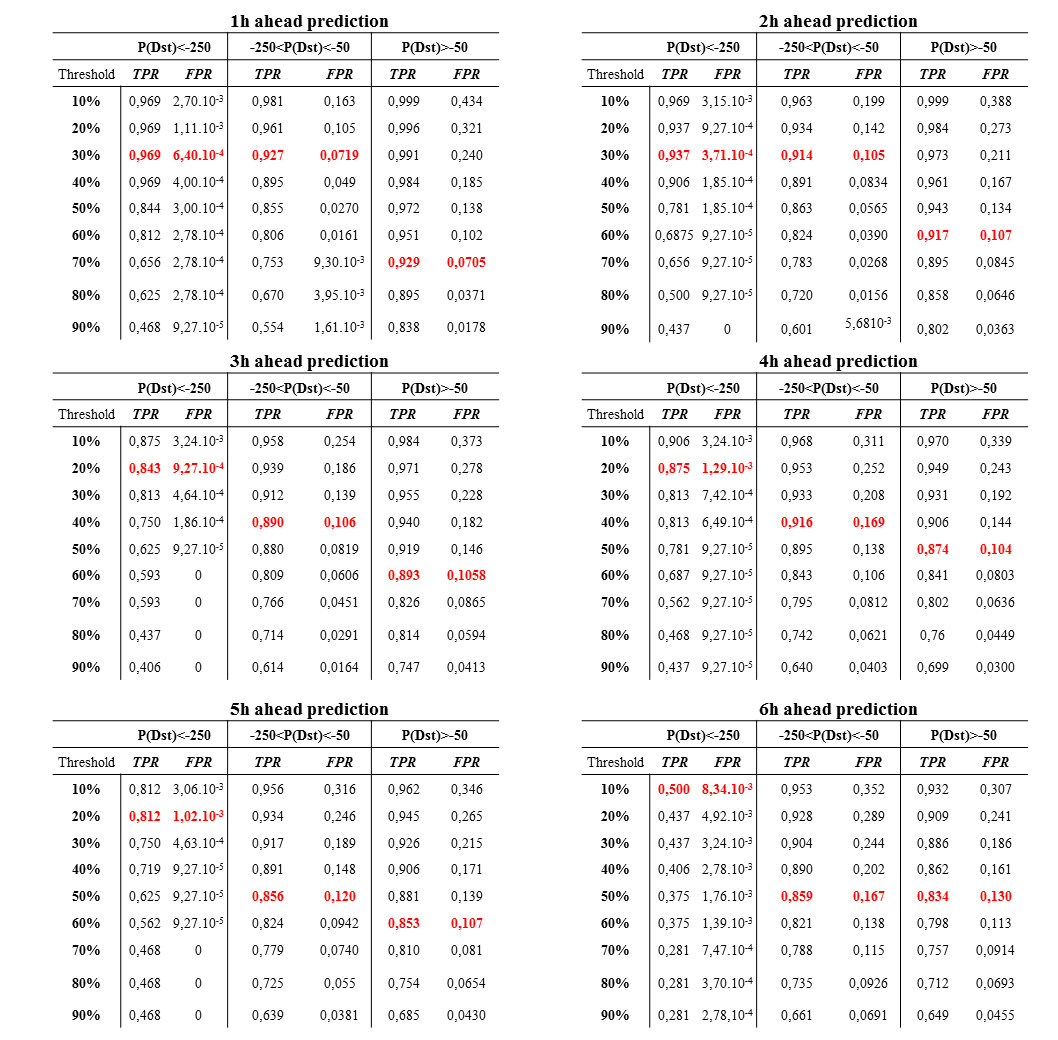
\includegraphics[width=\textwidth]{image1.png}
	\caption{False and True positive ratios for each storm category. The optimal value is in bold and red.}
	\label{fig:tpfp}
\end{figure}


%%%%%%%%%%%%%%%%%%%% Figure/Image No: 1 Ends here %%%%%%%%%%%%%%%%%%%%


%%%%%%%%%%%%%%%%%%%% Figure/Image No: 2 starts here %%%%%%%%%%%%%%%%%%%%

\begin{figure}
	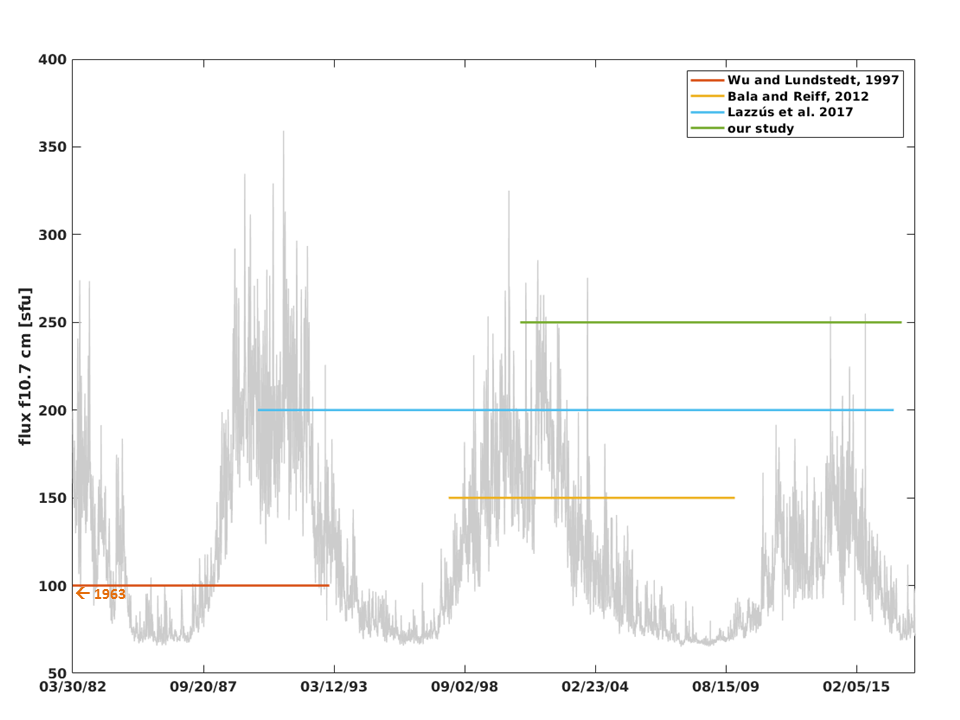
\includegraphics[width=\textwidth]{image2.png}
	\caption{Temporal coverage of database used in this study and in previous studies. Wu and Lundstedt [1997] is in orange and their database starts in 1963, Bala and Reiff [2012] is in yellow, Lazzús et al. [2017] is in blue, and our study is in green. The f10.7 in grey represents the variation of solar activity.}
	\label{fig:datacoverage}
\end{figure}


%%%%%%%%%%%%%%%%%%%% Figure/Image No: 2 Ends here %%%%%%%%%%%%%%%%%%%%


%%%%%%%%%%%%%%%%%%%% Figure/Image No: 3 starts here %%%%%%%%%%%%%%%%%%%%

\begin{figure}
	\noindent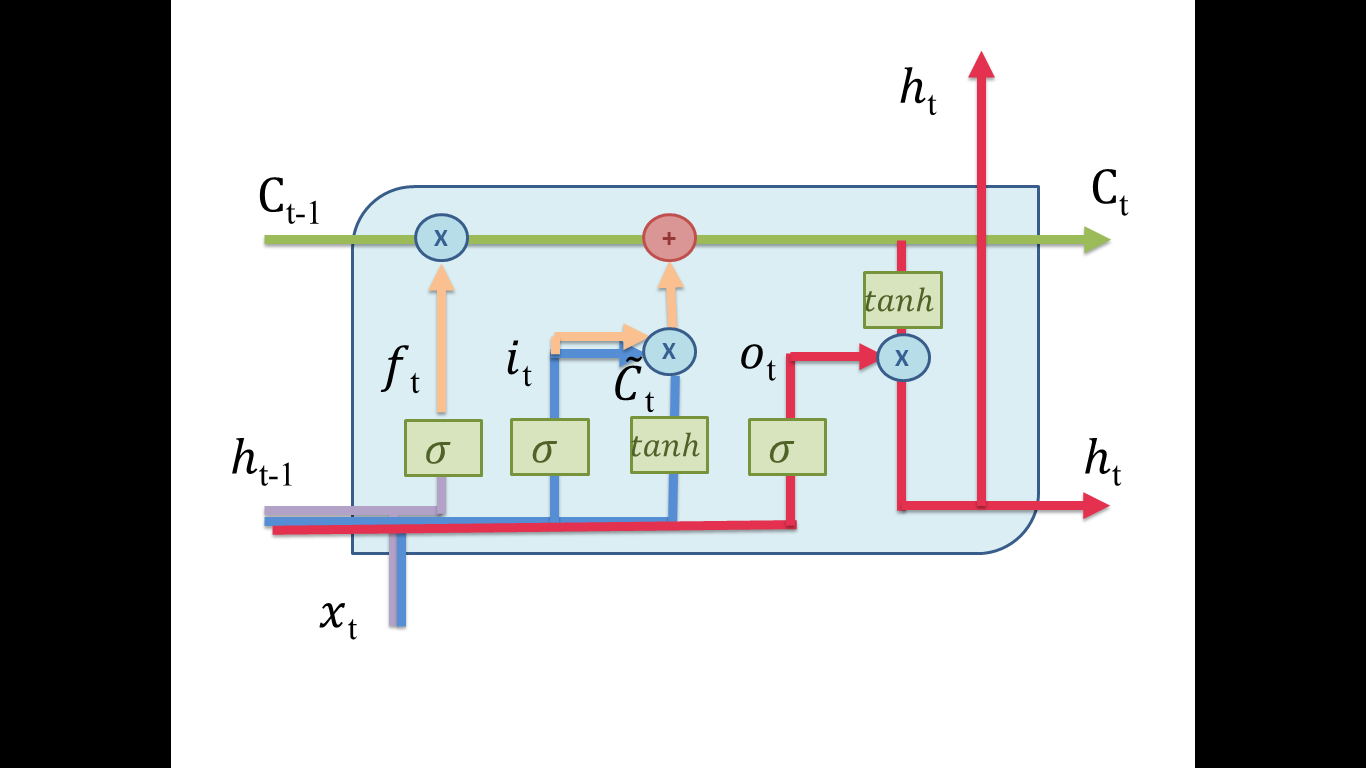
\includegraphics[width=\textwidth]{image3.png}
	\caption{LSTM cell. The cell state is in green, the forget gate in purple, the input gate in blue, and the output gate in red.}
	\label{fig:lstmcell}
\end{figure}


%%%%%%%%%%%%%%%%%%%% Figure/Image No: 3 Ends here %%%%%%%%%%%%%%%%%%%%



%%%%%%%%%%%%%%%%%%%% Figure/Image No: 4 starts here %%%%%%%%%%%%%%%%%%%%

\begin{figure}
	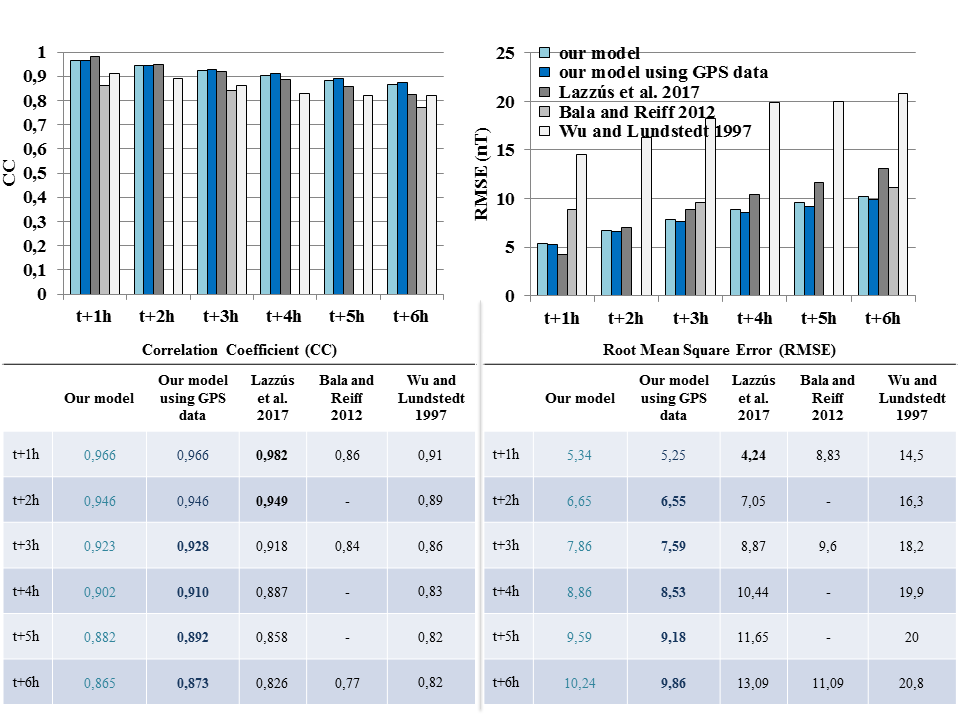
\includegraphics[width=\textwidth]{image4.png}
	\caption{LSTM performance in comparison to previous models. Our model with and without GPS data is highlighted in blue.}
	\label{fig:lstmperf}
\end{figure}


%%%%%%%%%%%%%%%%%%%% Figure/Image No: 4 Ends here %%%%%%%%%%%%%%%%%%%%



%%%%%%%%%%%%%%%%%%%% Figure/Image No: 5 starts here %%%%%%%%%%%%%%%%%%%%

\begin{figure}
	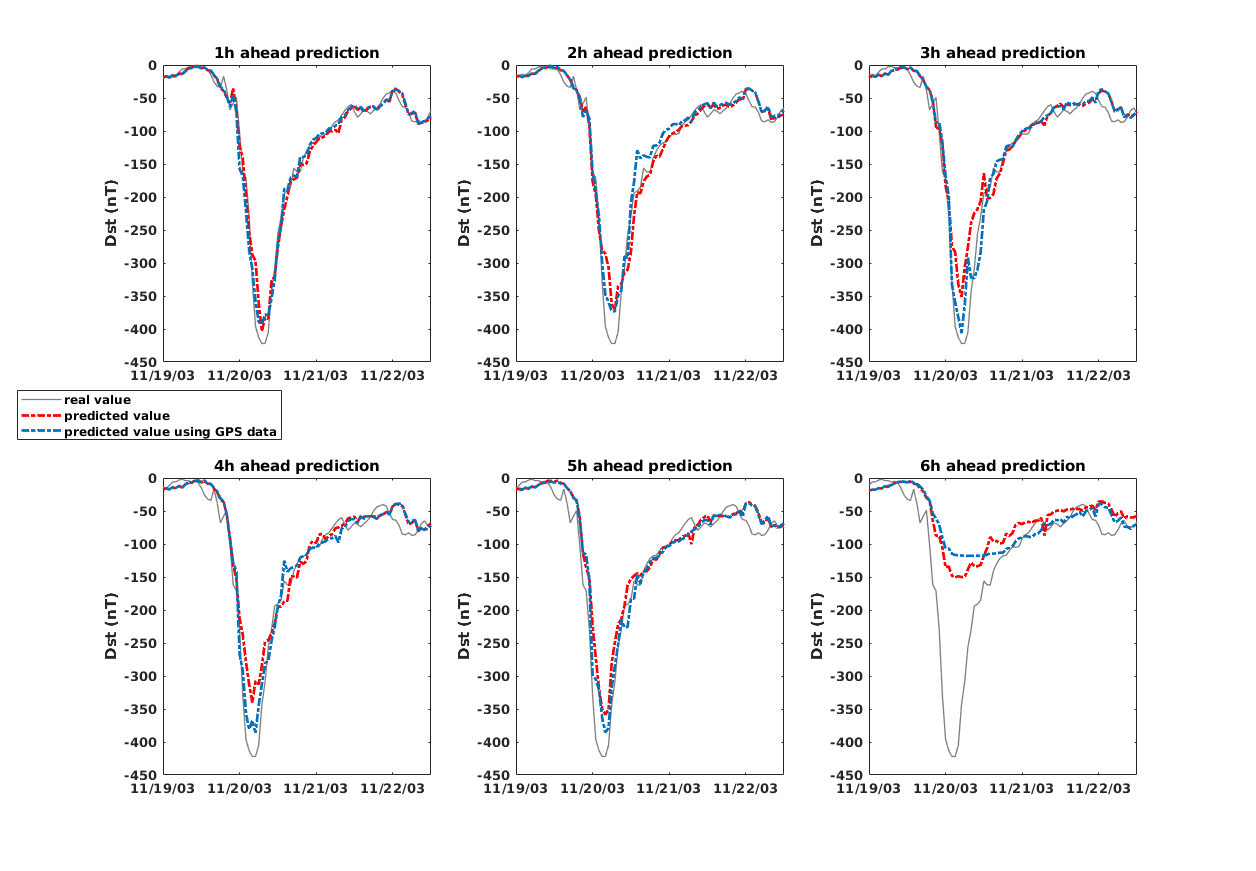
\includegraphics[width=\textwidth]{image5.png}
	\caption{LSTM predictions without GPS data (in red dot line) and with GPS data (in blue dot line) for the 2003 Halloween storm. The real value is the grey line.}
	\label{fig:lstmpredswoGPS}
\end{figure}


%%%%%%%%%%%%%%%%%%%% Figure/Image No: 5 Ends here %%%%%%%%%%%%%%%%%%%%


%%%%%%%%%%%%%%%%%%%% Figure/Image No: 6 starts here %%%%%%%%%%%%%%%%%%%%

\begin{figure}
	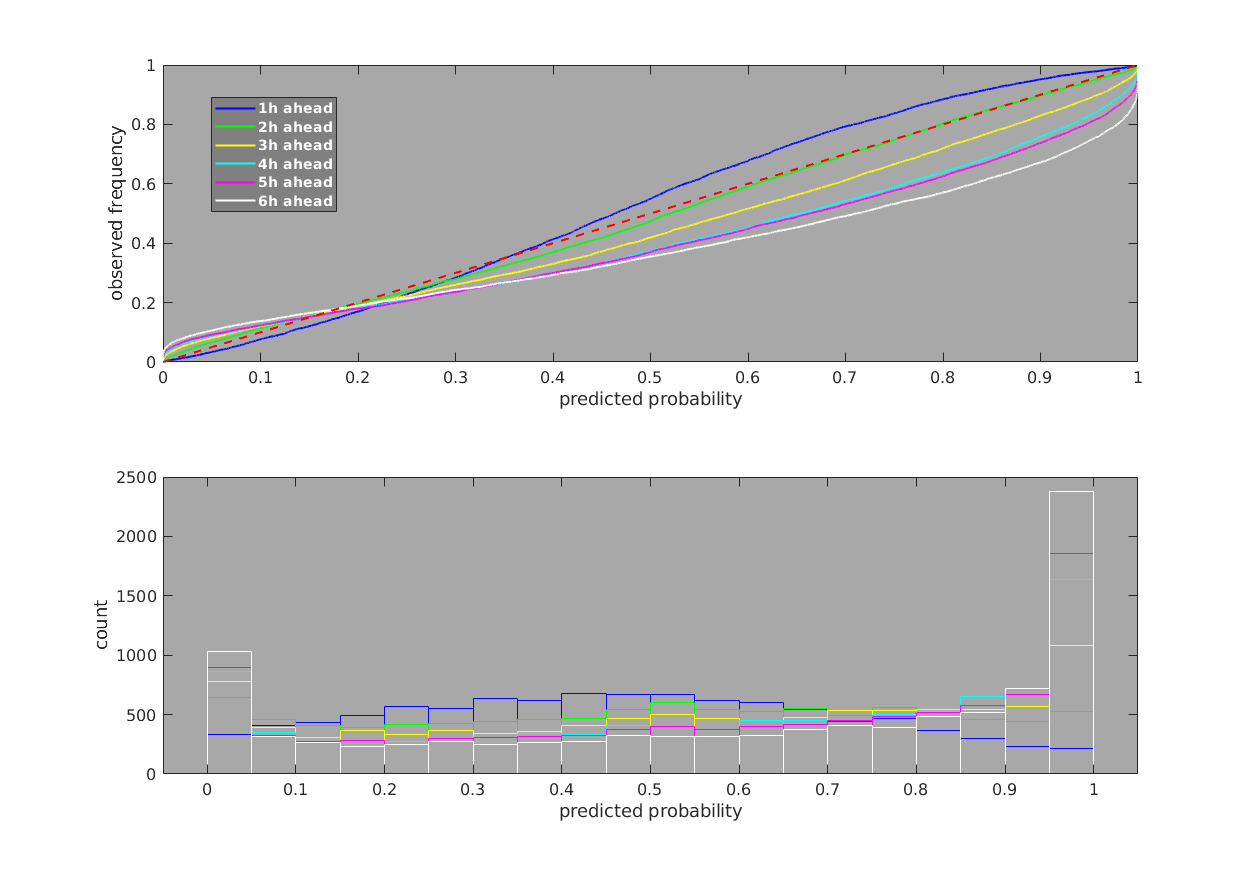
\includegraphics[width=\textwidth]{image6.png}
	\caption{Reliability diagram for Dst forecast from 1h ahead to 6h ahead. The diagonal is in red dot line.}
	\label{fig:gpnnreliability}
\end{figure}


%%%%%%%%%%%%%%%%%%%% Figure/Image No: 6 Ends here %%%%%%%%%%%%%%%%%%%%



%%%%%%%%%%%%%%%%%%%% Figure/Image No: 7 starts here %%%%%%%%%%%%%%%%%%%%

\begin{figure}
	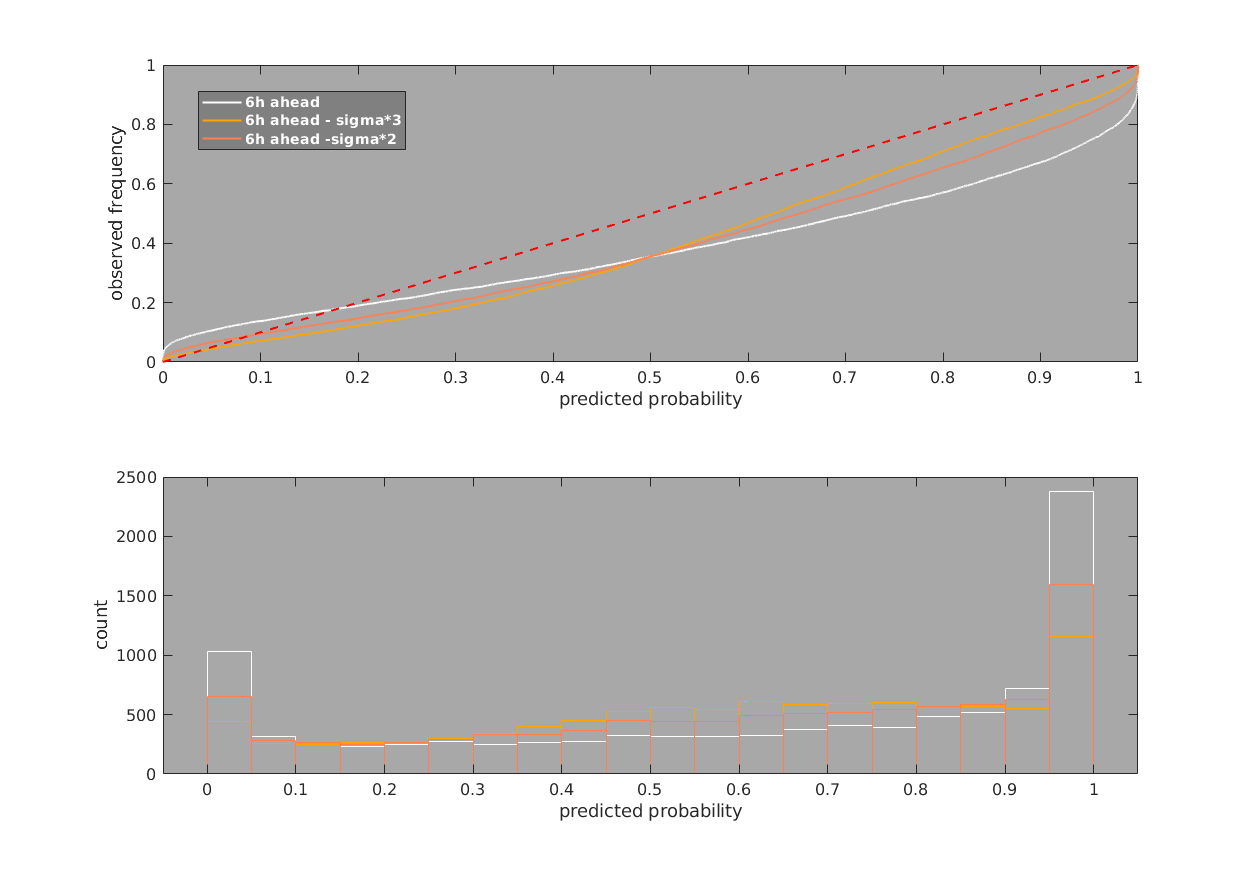
\includegraphics[width=\textwidth]{image7.png}
	\caption{Reliability diagram for the Dst prediction depending on the sigma value. The diagonal is in red dot line.}
	\label{fig:gpnnreliabilitysigma}	
\end{figure}


%%%%%%%%%%%%%%%%%%%% Figure/Image No: 7 Ends here %%%%%%%%%%%%%%%%%%%%

%%%%%%%%%%%%%%%%%%%% Figure/Image No: 8 starts here %%%%%%%%%%%%%%%%%%%%

\begin{figure}
	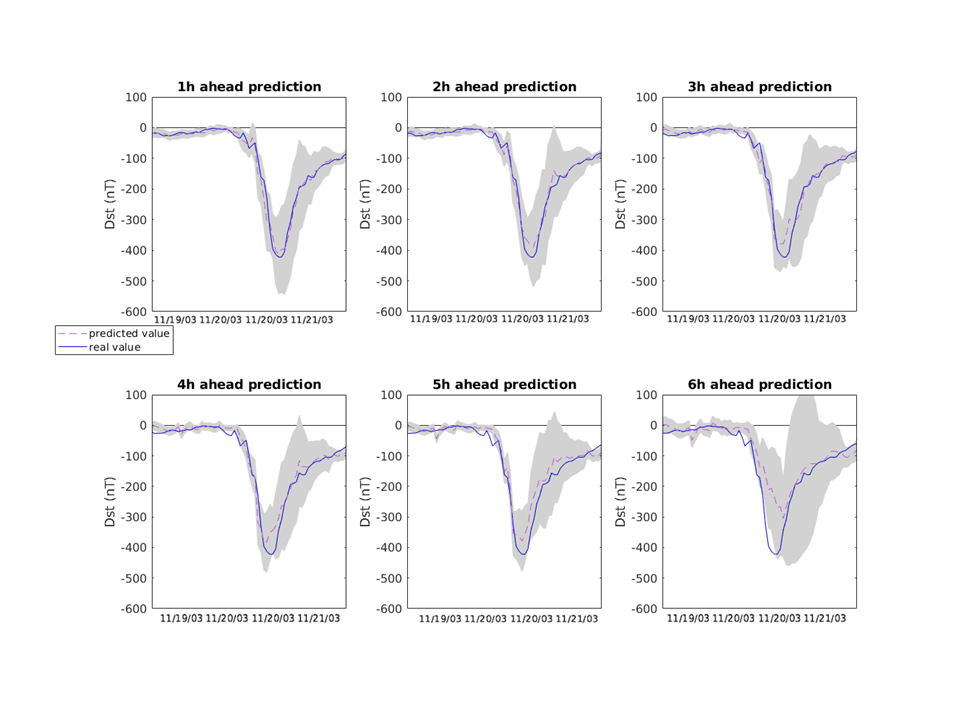
\includegraphics[width=\textwidth]{image8.png}
	\caption{GPNN performance to predict Dst for the 2003 Halloween storm. The predicted value is the purple dot line. The real value is the deep blue line The covariance is the grey shadow.}
    \label{fig:gpnnhalloween}
\end{figure}


%%%%%%%%%%%%%%%%%%%% Figure/Image No: 8 Ends here %%%%%%%%%%%%%%%%%%%%



\bibliographystyle{plain}
\bibliography{references}

\clearemptydoublepage

\chapter{Bayesian Inference of Plasma Diffusion Parameters}\label{chapter:bayes_diff_chapter}

{\small
  We present a novel method which combines sparse irregular observations of a field with its governing 
  physical dynamics, for performing Bayesian inference over latent system parameters. Our method uses 
  a basis function approach coupled with a least squares support vector machine objective function which 
  weighs differently errors arising due to data fitting and satisfaction of physical constraints. The method 
  is applicable to linear PDE systems, it incorporates physical models into classical least squares techniques 
  for the purpose of data assimilation and uncertainty quantification of latent parameters. We apply this method 
  to the inverse problem of inferring uncertainty estimates of plasma diffusion parameters from sparse observations.
}

\vfill
\sectionlinetwo{DarkGreen}{88}
\vfill

\noindent
    \parbox{\textwidth}{%
        {\small This chapter is based on research which is in preperation for publication.}
    }%


\clearpage


\section{Introduction}

The Earth's radiation belts are the regions of space near 
the Earth that extend between 2 and 8 Earth's radii, where the terrestrial magnetic field traps 
electrons and ions in complex electromagnetic orbits  \citep{vanAllen}. Since their discovery,
the belts have been the subject of intensive research due to their complex behavior
and damaging effects on spacecraft \citep{GUBBY20021723, WellingSatellite, baker2002}.

Radiation belt particles generally execute three types of periodic motion, 
each with its own corresponding adiabatic invariant: 
gyration about magnetic field lines, bounce along field lines, 
and drift around the Earth. During active times, when conditions 
change on time scales shorter than the periods of motion, 
adiabaticity can be broken and particle motion can not be
simply decomposed into the aforementioned components. Particle motion 
can then be represented diffusively along each component via the 
\emph{Fokker-Planck} equation yielding a powerful picture of 
radiation belt dynamics \citep{schulz2012particle}.

The third invariant represents the total magnetic flux enclosed within 
a full particle orbit. It is common to use a normalized form of this, the 
so called Roederer $L^{*}$ \citep{Roederer1970}. It is analogous to radial 
distance from the center of the Earth (in Earth radii) to the equatorial 
crossing point of the bouncing particle. Diffusion in $L^{*}$ alone 
(the other invariants shall be considered conserved) accounts for the
capture and inward radial transport of radiation belt particles 
\citep{Roederer1970,JGR:JGR4463}.

One of the main difficulties of using a physics-based model for studying and 
forecasting energetic electrons in the radiation belt is that the parameters 
that characterize the Fokker-Planck equation, namely diffusion tensor and loss term,
are not directly observable. Hence, their determination represents an inverse problem,
which is generally difficult to solve and can often become ill-posed.

In this paper we propose an inference model which can learn from sparse
data while taking into account prior knowledge of the system dynamics
in the form of a linear partial differential equation. The method replaces
the finite difference solver with a surrogate model which tries to fit
the observations and the system dynamics. The surrogate is expressed as
a basis function expansion whose coefficients are computed by formulating
a \emph{Least Squares Support Vector Machine}(LSSVM) like optimization
objective.

In the proceeding sections, we give a short introduction to the radial 
diffusion equation used in magnetospheric physics. After an overview of 
the parameterizations of the radial diffusion unknowns used by the research community, 
we give a detailed formulation of our proposed method and demonstrate 
how one may use it for performing inference over said diffusion parameters.

\subsection{Plasma Diffusion}

The radial diffusion system is a simplified one-dimensional version of
the \emph{Fokker-Planck} equation. It tracks the time evolution of the
\emph{phase space density} of particles, $f$ which is governed by 
\cref{eq:raddiffusion} known as \emph{radial diffusion equation} in the 
radiation belt community \citep{JGRA:JGRA9345}.

\begin{equation}\label{eq:raddiffusion}
  \frac{\partial{f}}{\partial{t}} = l^2 \frac{\partial}{\partial{l}}\left( \frac{\kappa(l,
      t)}{l^{2}} \frac{\partial{f}}{\partial{l}} \right) - \lambda(l,
  t) f +  Q(l, t)
\end{equation}

The \emph{phase space density} $f$ is a function of the spatial
coordinate $l$ which denotes the \emph{Roederer} $L^*$ or
\emph{L-shell}, and time $t$.

The key quantities in the system above are.

\begin{enumerate}
\item $f$: The density of particles as a function of space $l$ and
  time $t$.
\item $\kappa(l, t)$: Diffusion field.
\item $\lambda(l, t)$: Loss rate, this is a non-negative
  quantity which indicates how quickly particles are lost from the
  radiation belts.
\item $Q(l, t)$: Particle injection rate.
\end{enumerate}

\subsubsection*{Diffusion Parameters}

To solve the radial diffusion system (\cref{eq:raddiffusion}), the
quantities $\kappa(l, t)$, $\lambda(l, t)$ and $Q(l, t)$ need to be
specified. It is a common practice \citetext{see \citealp{GRL:GRL10762},
\citealp{JGRA:JGRA15067}, \citealp{JGRA:JGRA18021} and
\citealp{GRL:GRL22815}} to parameterise the diffusion field
$\kappa$ and loss rate $\lambda$ in the following manner.

\begin{align}
  \kappa(l,t), \lambda(l, t) \sim \alpha l^{\beta} 10^{b Kp(t)} \\
\end{align}

The quantities $\alpha$, $\beta$ and $b$ are parameters which define
the diffusion field and loss rate while the quantity $Kp(t)$ is known
as the Kp index, a measured quantity which stands as a proxy for the
global geomagnetic activity \citep{BartelsKp}.


\section{Inverse Problems}\label{sec:inv}

The \emph{inverse problem} can be stated as follows: given a set of
noisy observations $y$ scattered in the space time domain, of a
physical quantity $f$ governed by the dynamical system
$\mathcal{L}_{\theta} f = Q_{\theta}$, estimate the parameters $\theta$ of the
dynamical system $(\mathcal{L}_{\theta}, Q_{\theta})$.

In this formalism $\mathcal{L}_{\theta}$ is a differential operator,
$Q_{\theta}$ is a \emph{source term} and $\theta$ is a collection of parameters
which specify the operator and the source term.

In the radial diffusion system (\cref{eq:raddiffusion}), $\mathcal{L}_{\theta} =
\frac{\partial}{\partial{t}} - l^2 \frac{\partial}{\partial{l}}\left( \frac{\kappa(l,
      t)}{l^{2}} \frac{\partial}{\partial{l}} \right) + \lambda(l,
  t)$. In this case $\theta$ would be a collection of parameters which
  would specify the analytic expressions for $\kappa(l,t)$,
  $\lambda(l,t)$ and $Q(l,t)$.

\subsection{Related Work}

\subsubsection*{Meshfree PDE solutions}

\paragraph{Least Squares Support Vector Machines}

(LSSVM) have been applied to calculating approximate solutions to PDEs
\citep{MEHRKANOON2015105,MEHRKANOON20122502} as well as
parameter estimation of delay differential equations
\citep{MEHRKANOON2014830}, the approach taken in the aforementioned
research \citep{MEHRKANOON2014830} was expressing the parameter
estimation of time delay as an algebraic optimization problem
resulting in closed-form approximation for the time varying parameters
while avoiding iterative simulation of the dynamical system (governed
by the delay differential equations) in the parameter estimation process.

\paragraph{Radial Basis Functions}

(RBF) were first applied for solution of PDE problems in \citet{KANSA1990147}, 
the authors used colocation with \emph{multiquadric} basis functions for approximating solutions
of boundary value problems.

Radial basis functions have been applied for the mesh-free solutions of Poisson PDE systems 
\citep{AMINATAEI20082887,DUAN200866,DUAN2006394,CNM:CNM419}, as well as the Poisson control problem 
\citep{Pearson2013}. Further applications of RBFs include atmospheric flow \citep{Tillenius2015406}, 
convection-diffusion \citep{Safdari-Vaighani2015}, and Schrödinger's equation \citep{doi:10.1137/120893975}. 
Refer to \citet{fornberg2015} for a recent textbook with geoscience applications.

\paragraph{Gaussian Processes}

Gaussian Process (GP) models \citep{Rasmussen:2005:GPM:1162254} have a rich theory which has much overlapping 
with linear systems and deterministic and stochastic differential equations. 

\citet{Skilling1992} presented one of the earliest works which focused on calculating solutions of ordinary 
differential equations (ODE) systems with Gaussian Process methodology, \citet{Graepel} applied it for solving 
linear partial differential equations with Dirichlet and Von Neumann boundary conditions.

Interplay between linear operators and GP models applied to Bayesian filtering was investigated by \citet{Sarkka2011}. 
\citet{pmlr-v31-dondelinger13a} proposed an adaptive gradient matching technique to used Gaussian Process models for 
infering parameters of coupled ODE systems.

\paragraph{Neural Networks} were also employed for solutions of boundary value problems in the works such as 
\citet{Lagaris,Aarts2001,TSOULOS20092385,Baymani2011} which used Feedforward networks for 
calculating solutions to the Stokes problem. These approaches generally revolved around decomposing the solution 
into two components, i.e. the first one satisfying the boundary conditions and the second one represented by the 
feedforward network.


\section{Methodology}

Performing Bayesian inference over parameters of physical systems,
involves synthesizing pre-exsiting knowledge of the physical system in
question i.e. the \emph{partial differential equation} (PDE), with
statistical techniques. The aim of such an exercise is often the
quantification of uncertainty over system parameters from an often
sparse set of observations which are quantities of interest in the
physical system. 


\subsection{Model Formulation}

We approach the radial diffusion inference problem by formulating a
modified version of the \emph{least squares support vector machine}
predictor for obtaining a closed form approximation to the phase space
density $f$ which tries to satisfy the radial diffusion PDE
(\cref{eq:raddiffusion}) on a fixed set of \emph{colocation} points while
minimizing error on a set of sparse noisy observations. 
Using the surrogate phase space density estimator as a baseline, we
specify the likelihood of the observations.


\subsubsection*{Surrogate Phase Space Density Model}

Let $\mathcal{D}={(x^{o}_{i}, y_{i}): i = 1 \cdots n_{o}}$ be a set of
noisy observations of the phase space density $f$, where $x_{i} =
(l_{i}, t_{i})$ are points in the space time domain. We seek a linear
estimator for $f$ of the form $\hat{f}(x) = w^{T}\varphi(x) + b$,
where $\varphi(.): \mathbb{R}^{2} \rightarrow \mathbb{R}^{d}$ is a $d$
dimensional feature map and $b$ is a scalar intercept.

Further let $\mathcal{C} ={(x^{c}_{i}, q_{i}): i = 1 \cdots n_{c}}$ be 
a set of colocation points on which we aim to enforce radial diffusion
dynamics. The values $q_{i}$ represent the particle injection rate $Q$ at $x^c$ and 
are calculated each time the parameters of Q are sampled, by evaluating the expression 
$Q(l,t) = (\alpha_{Q}l^{\beta_{Q}} + \gamma_{Q})10^{b_{Q}Kp(t)}$.

We exploit the linearity of the differential operator
$\mathcal{L}_{\theta}$ and note that $\mathcal{L}_{\theta} [\hat{f}(x)]
= w^{T} \mathcal{L}_{\theta}[\varphi(x)]$, yielding an estimator
$\hat{Q}(x) = w^{T}\psi(x)$ where $\psi_{\theta}(x) =
\mathcal{L}_{\theta}[\varphi(x)]$. Calculating $w \in \mathbb{R}^d$
can now be cast as the following constrained $L_2$ regularized 
least squares problem.

\begin{align}\label{eq:surrogate}
   & min_{w,e,\epsilon} \ \mathcal{J}(w,e,\epsilon;\theta) = \\
   & \frac{1}{2} w^{T}w + \frac{1}{2\gamma_{o}} \sum_{k = 1}^{n_{o}}{e^{2}_{k}} + \frac{1}{2\gamma_{c}} \sum_{k = 1}^{n_{c}}{u_{k} \epsilon^{2}_{k}} \\
  s.t &\nonumber \\
  & y_{i}  = w^{T}\varphi(x^{o}_{i}) + b + e_{i}, \ \ i = 1 \cdots n_{o} \\
  & q_{i} = w^{T}\psi_{\theta}(x^{c}_{i}) + \epsilon_{i}, \ \ i = 1 \cdots n_{c}
\end{align}

It can be seen that system in \cref{eq:surrogate} is similar to the
formulation of the LSSVM model, while incorporating the dynamics of
linear PDE systems into its loss function. 

The quantities $\gamma_{o}$ and $\gamma_{c}$ are weights attached to
the errors on observations and colocation points respectively, thus
by smoothly varying them one may assign higher or lower importance for
the surrogate model to fit the observational data and the dynamics of
the physical system. The quantities $u_i$ enable us to weigh each colocation
point differently.

In order to solve this system one must construct its
\emph{Lagrangian}.

\begin{align*}\label{eq:lag}
      & \mathfrak{L}(w,e,\epsilon, \alpha_{1 \cdots k}, \beta_{1 \cdots k}; \theta; \gamma_{o}; \gamma_{c}) = \\ 
      & \frac{1}{2} w^{T}w + \frac{1}{2\gamma_{o}} \sum_{k = 1}^{n_{o}}{e^{2}_{k}} +
      \frac{1}{2\gamma_{c}} \sum_{k = 1}^{n_{c}}{u_{k} \epsilon^{2}_{k}} \\
      & + \sum_{k = 1}^{n_{o}}{\alpha_{k}(y_{k} - w^{T}\varphi(x^{o}_{k}) - b - e_{k})} \\
      & + \sum_{k = 1}^{n_{c}}{\beta_{k} (q_{j} - w^{T}\psi_{\theta}(x^{c}_{j}) - \epsilon_{j})} 
\end{align*}

Given fixed values for $\gamma_{o}$, $\gamma_{c}$ and PDE parameters
$\theta$, the equation above expresses the Lagrangian of the system in 
\cref{eq:surrogate}. The quantities $\alpha_{1}, \cdots, \alpha_{n_{o}}$ and
$\beta_{1}, \cdots, \beta_{n_{c}}$ are the \emph{Lagrange multipliers}
introduced for equality constraints of the system. Applying the
\emph{Karush-Kuhn-Tucker}(KKT) conditions, the solution of the
optimization problem in \cref{eq:surrogate} can be expressed in terms of
the Lagrange multipliers $\alpha = (\alpha_{1}, \cdots, \alpha_{n_{o}})$
$\beta = (\beta_{1}, \cdots, \beta_{n_{c}})$.

\begin{equation}\label{eq:solution}
  \begin{bmatrix}
    0 & \mathbf{1}^{T} & \mathbf{0} \\ 
    \mathbf{1} & \Omega + \gamma_{o}I  & \Omega_*\\ 
    \mathbf{0} & \Omega_{*}^{T}  & \Omega_{**} + \gamma_{c}U 
  \end{bmatrix} \begin{bmatrix}
    b\\ 
    \alpha\\ 
    \beta
  \end{bmatrix} = \begin{bmatrix}
    0\\ 
    y\\ 
    q
  \end{bmatrix}
\end{equation}

The components of the symmetric block matrix system on the left hand side of 
\cref{eq:solution} are 
\begin{enumerate}
\item $\Omega \in \mathbb{R}^{n_{o} \times n_{o}}: \omega_{ij} = \varphi(x^{o}_{i})^{T} \varphi(x^{o}_{j})$
\item $\Omega_{**} \in \mathbb{R}^{n_{c} \times n_{c}}: \omega^{**}_{ij} = \psi(x^{c}_{i})^{T} \psi(x^{c}_{j})$
\item $\Omega_{*} \in \mathbb{R}^{n_{o} \times n_{c}}: \omega^{*}_{ij} = \varphi(x^{o}_{i})^{T} \psi(x^{c}_{j})$
\item $U \in \mathbb{R}^{n_{c} \times n_{c}} = \begin{bmatrix}
    u_1 & \cdots & 0 \\ 
    \vdots & \ddots  & 0\\ 
    0 & \cdots  & u_{n_{c}} 
  \end{bmatrix}$
\end{enumerate}

The surrogate model can now be used to estimate the phase space density 
at a point $x = (l,t)$.

\begin{equation}\label{eq:model}
\hat{f}(x;\theta) = \sum_{k = 1}^{n_{o}}{\alpha_{k}\varphi(x)^{T}\varphi(x^{o}_{k}) + \sum_{k = 1}^{n_{c}}}{\beta_{k} \varphi(x)^{T} \psi_{\theta}(x^{c}_{k})} + b
\end{equation}

\subsubsection*{Choice of Basis}

There exist several choices regarding the basis $\varphi(.)$, they are but not limited to 
orthogonal polynomials, Fourier series, radial basis functions etc. 

For our problem we choose a basis which is a product of a Chebyshev basis of maximum degree 10 in space and a Laguerre basis of maximum degree 4, in time.

\begin{equation}\label{eq:basis}
\varphi_{i,j}(l,t) = C_{i}(l) L_{j}(t)
\end{equation}



\subsubsection*{Role of $\gamma_o$, $\gamma_c$ and $u_i$}

The quantities $\gamma_o$ and $\gamma_c$ serve to control the importance assigned to
of errors made on the observations and colocation points respectively. Varying them 
gives the modeler the ability to vary the behavior of the surrogate model. In the 
limiting case of $\gamma_c$ tending to zero, the model behaves as if the PDE dynamics
is enforced as a hard constraint. This case is equivalent to the following formulation.

\begin{align}\label{eq:surrogate2}
   min_{w,e} \ \mathcal{J}(w,e,\epsilon;\theta) &= 
   \frac{1}{2} w^{T}w + \frac{1}{2\gamma_{o}} \sum_{k = 1}^{n_{o}}{e^{2}_{k}} \\
  & s.t \nonumber \\
  y_{i} & = w^{T}\varphi(x^{o}_{i}) + b + e_{i}, \ \ i = 1 \cdots n_{o} \\
  q_{i} & = w^{T}\psi_{\theta}(x^{c}_{i}), \ \ i = 1 \cdots n_{c}
\end{align}

Although choosing $\gamma_c = 0$ is an appropriate choice if one wishes
to enforce the physical dynamics as a constraint, it can possibly lead to numerical
instabilities in inverting system in \cref{eq:solution} and hence choosing a non zero value 
for $\gamma_c$ works better in practice.

For the experiment outlined in \ref{sec:exp}, we choose $\gamma_o = \gamma_c = 10$.

The weights $u_i$ have a special interpretation in a particular context. It is possible to
interpret the term $\sum_{k = 1}^{n_{c}}{u_{k} \epsilon^{2}_{k}}$ as a quadrature approximation
to the integrated error of the surrogate model with respect to the governing dynamics $\int_{x \in \mathcal{D}}{||\mathcal{L}_{\theta} [\hat{f}(x)] - Q(x)||^2}$. When
$u_i = \frac{1}{n_c}$, this corresponds to the \emph{Monte Carlo} quadrature of 
the integrated error, but it is possible to improve the quadrature accuracy by using \emph{Gauss-Legendre} quadrature.

In section \ref{sec:exp}, we use eight point \emph{Gauss Legendre} quadrature in space and time dimension each, thereby setting $n_c = 64$ and weights $u_i$ to appropriate values as dictated by the quadrature rule (\citet{_abramowitzm}).

\subsection{Quantifying Observation Likelihood}

We assume a multivariate Gaussian distribution for calculating the likelihood of 
the observations conditioned on the system parameters $\theta$. 

The surrogate model (\cref{eq:model}) gives a baseline or mean value for the phase space density, we use a
hybrid RBF covariance function $C(x_{i}, x_{j}) = \sigma^2 exp(-\frac{1}{2} (\frac{|l_i - l_j|^2}{s} + \frac{|t_i - t_j|}{r}))$
to quantify the covariance of the phase space density $f$ over two points 
$x_i = (l_i, t_i)$ and $x_j = (l_j, t_j)$ in the domain. 

\begin{equation}
\mathbf{y} | x_1, \cdots, x_{n_o}, \theta \sim \mathcal{N} \left(\mathbf{\mu}_f, \Sigma \right )
\end{equation}

\begin{equation}
\mathbf{y} = \begin{bmatrix}
y_1\\ 
\vdots\\ 
y_{n_o}
\end{bmatrix}
\end{equation}

\begin{equation}
  \mathbf{\mu}_f = \begin{bmatrix}
\hat{f}(x_1)\\ 
\vdots\\ 
\hat{f}(x_{n_o})
\end{bmatrix}
\end{equation}

\begin{equation}
    \Sigma = \begin{bmatrix}
C(x_1, x_1) & \cdots  & C(x_1, x_{n_o})\\ 
\vdots & \ddots & \vdots\\ 
C(x_{n_o}, x_{n_{1}}) & \cdots  & C(x_{n_o}, x_{n_{o}})
\end{bmatrix}
\end{equation}

The values of $s$ and $r$, the length scales of the covariance function, 
can be fixed to the size of the space-time grid of the radial basis functions, 
alternatively they can also be treated as system parameters which can be sampled 
by the inference procedure. Since the core aims of this research was the quantification
of the uncertainty over the parameters of the radial diffusion system, 
we treat the covariance function parameters as fixed.

\subsection{Inference}

We employ the adaptive Metropolis algorithm as proposed by \citet{haario2001}, for sampling
system parameters. The adaptive Metropolis algorithm adapts the exploration variance according
to the running sample statistics of the Markov Chain procedure.


\section{Experiment}\label{sec:exp}

For the purposes of the experiment, the parameters of $\kappa$ and $\lambda$ fixed while MCMC inference 
is performed on the parameters of $Q$. The prior distributions chosen for the parameters 
are shown in table \ref{tab:prior}. The posterior distribution over the parameters of $\lambda$ is 
sampled via adaptive Metropolis, the first 5000 samples are kept aside as the \emph{burn in} period
of the Markov Chain.

\begin{table}[t]
  \caption{Parameters: Prior}
  \label{tab:prior}
  \centering
  \begin{tabular}{ll}
    \hline
    \textbf{Parameter} & \textbf{Prior}\\
    \hline
    $\alpha$ & $Lognormal(0, 1)$ \\
    $\beta$  & $Lognormal(1, 1)$ \\ 
    $\gamma$ & $Lognormal(0, 1)$ \\ 
    $b$ & $\mathcal{N}(0, 1)$ \\
    \hline
  \end{tabular}
\end{table}


\subsection*{Data Generation}

The technique presented is applied on synthetic data generated using a radial diffusion solver, 
the ground truth values of the radial diffusion parameters are listed in table \ref{tab:ground-truth}.

A slightly modified parameterization is adopted for the particle injection $Q$ as shown in \cref{eq:q} below. The particle injection has a strictly time varying component due to presence of a constant $\gamma$.

\begin{equation}\label{eq:q}
Q(l,t)  \sim (\alpha l^{\beta} + \gamma) 10^{b Kp(t)}
\end{equation}

The initial phase space density $f(t = 0)$ and the time trajectory 
of the Kp index are assumed to be set as follows.

\begin{align}
f(t = 0) &= 4000 + 1000(C_{3}(l_*) - C_{5}(l_*)) \\
l_* &= 2\frac{l - l_{min}}{l_{max} - l_{min}} - 1 \\
Kp(t) &= \left\{\begin{matrix}
2.5 + 4t & 0 \leq t < 1.5\\ 
8.5 & 1.5 < t \leq 3\\ 
17.5-3t & 3 <  t \leq 5 \\ 
2.5 & 5 < t\\ 
\end{matrix}\right.
\end{align}

Where $C_n(.)$ is the is the Chebyshev polynomial of degree n. 
The evolution of the Kp index \citet{BartelsKp} is assumed such that it mimics a geomagnetic storm event. 

The radial diffusion solver is run for domain limits $l \in [1, 7], t \in [0, 5]$ with
200 bins in the spatial and 50 bins in the temporal domains respectively.

After the approximate solution profiles of $f$ are generated, the points are sub-sampled
uniformly such that 100 points lie in the interior of the domain and 30 points at the initial time step (t = 0) are selected. These observations are then perturbed by Gaussian noise to yield
the final observation set $\mathcal{D}$ which is fed, as training data to the surrogate model $\hat{f}(x)$.

\subsection*{Results}

The posterior inferred for parameters of the particle injection rate $Q$ \ref{fig:alpha}, 
\ref{fig:beta}, \ref{fig:gamma} and \ref{fig:b} respectively and the samples from each prior distribution are shown in \ref{fig:alphaprior}, \ref{fig:betaprior}, \ref{fig:gammaprior} and \ref{fig:bprior} respectively.

We see that the marginal posterior distributions of each parameter have high probability 
density near the ground truth, and that they are heavy tailed because there are often large 
regions of the parameter space which produce similar solutions for the phase space density $f$. 
Apart from identifying of parameters, the model also helps in significant reduction of uncertainty
from prior to posterior for the parameters $\beta$, $\gamma$ and $b$.

The strength of the proposed method is the ability to quantify the uncertainty in diffusion parameters from a sparse set of observations. Due to the formulation of the surrogate as a dual optimization problem, it allows the inference to scale well with respect to high dimensional basis function expansions. The method shows promise for parameter inference of physical systems and warrants further research in its improvement.


\begin{table}[t]
  \caption{Parameters: Ground Truth}
  \label{tab:ground-truth}
  \centering
  \begin{tabular}{lllll}
    \hline
    \textbf{Quantity}     & $\alpha$     & $\beta$ & $\gamma$ & $b$ \\
    \hline
    $Q$ & $1$  & $0.5$ & $0.05$  & $0.45$     \\
    $\kappa$  & $4.731 \times 10^{-10}$ & $10$  & $0$ & $0.506$ \\
    $\lambda$ & $0.3678$ & $0.5$  & $0$ & $-0.2$ \\
    \hline
  \end{tabular}
\end{table}

\begin{figure}[h]
\vspace{.3in}
\centerline{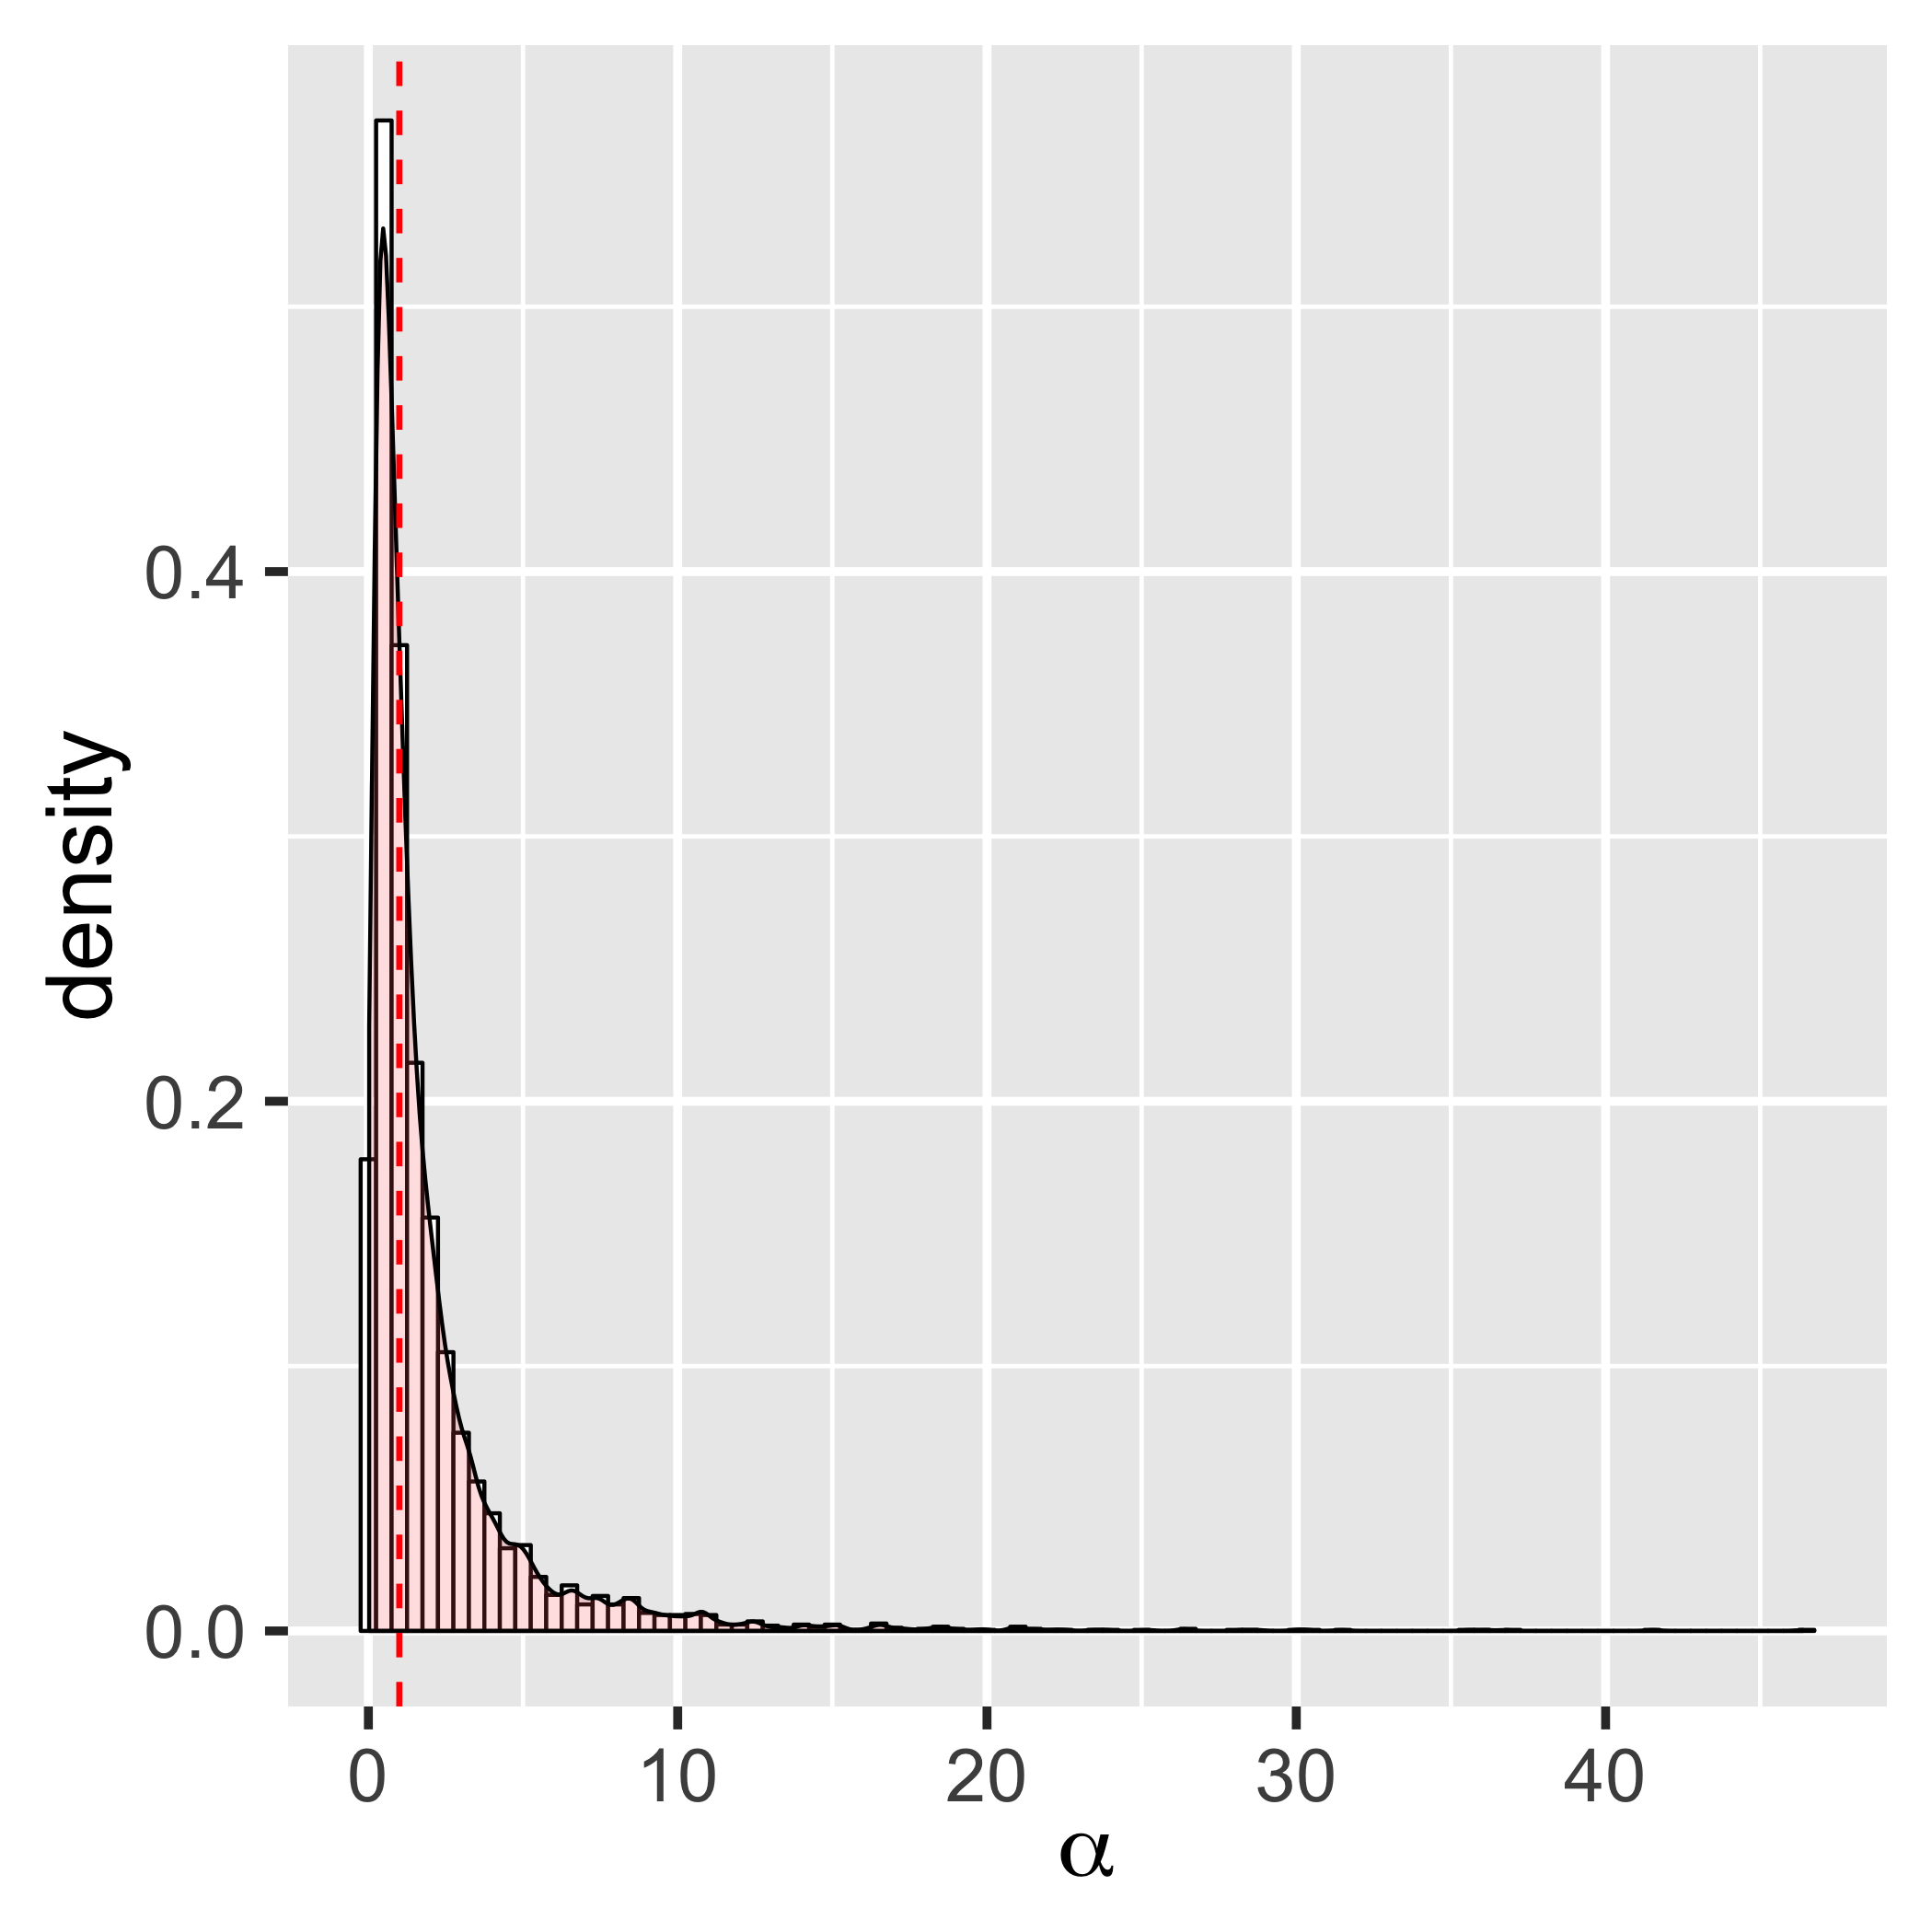
\includegraphics[width=0.5\textwidth]{histogram_Q_alpha_posterior.png}}
\vspace{.3in}
\caption{Posterior samples for $\alpha$ parameter of Q, red dotted line indicates the ground truth}
\label{fig:alpha}
\end{figure}

\begin{figure}[h]
\vspace{.3in}
\centerline{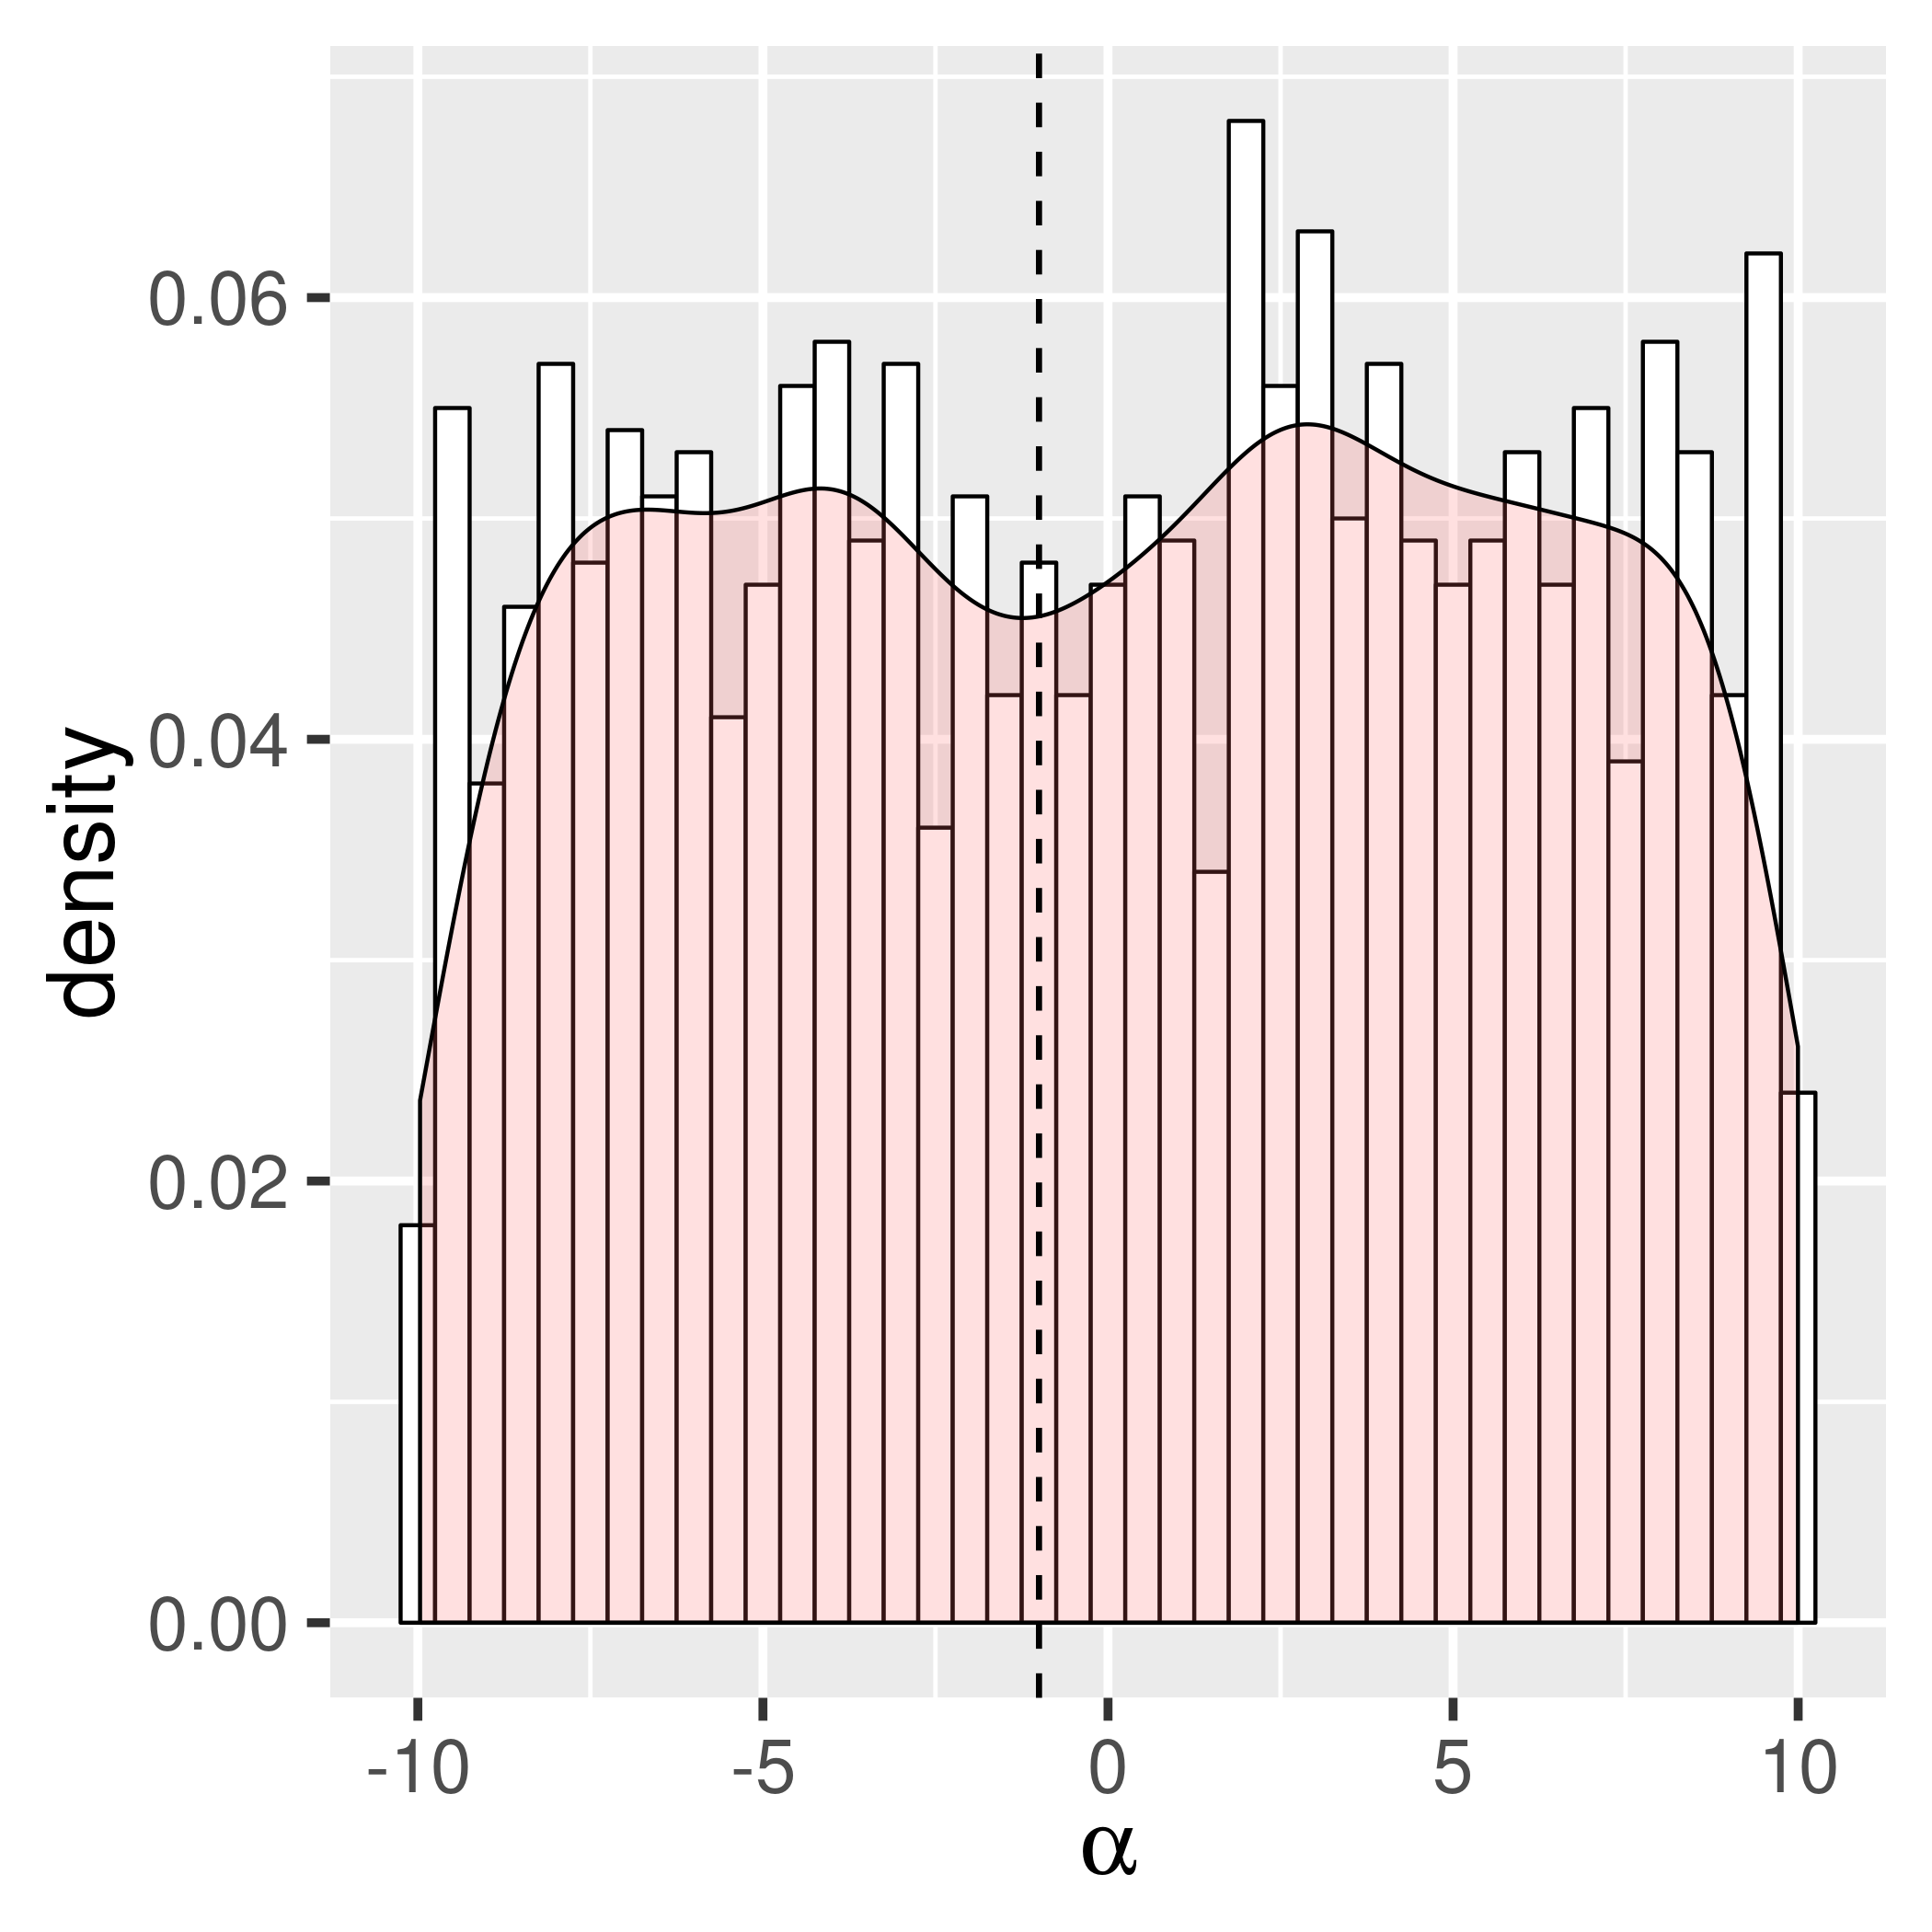
\includegraphics[width=0.5\textwidth]{histogram_Q_alpha_prior.png}}
\vspace{.3in}
\caption{Prior samples for $\alpha$ parameter of Q, red dotted line indicates the ground truth}
\label{fig:alphaprior}
\end{figure}

\begin{figure}[h]
\vspace{.3in}
\centerline{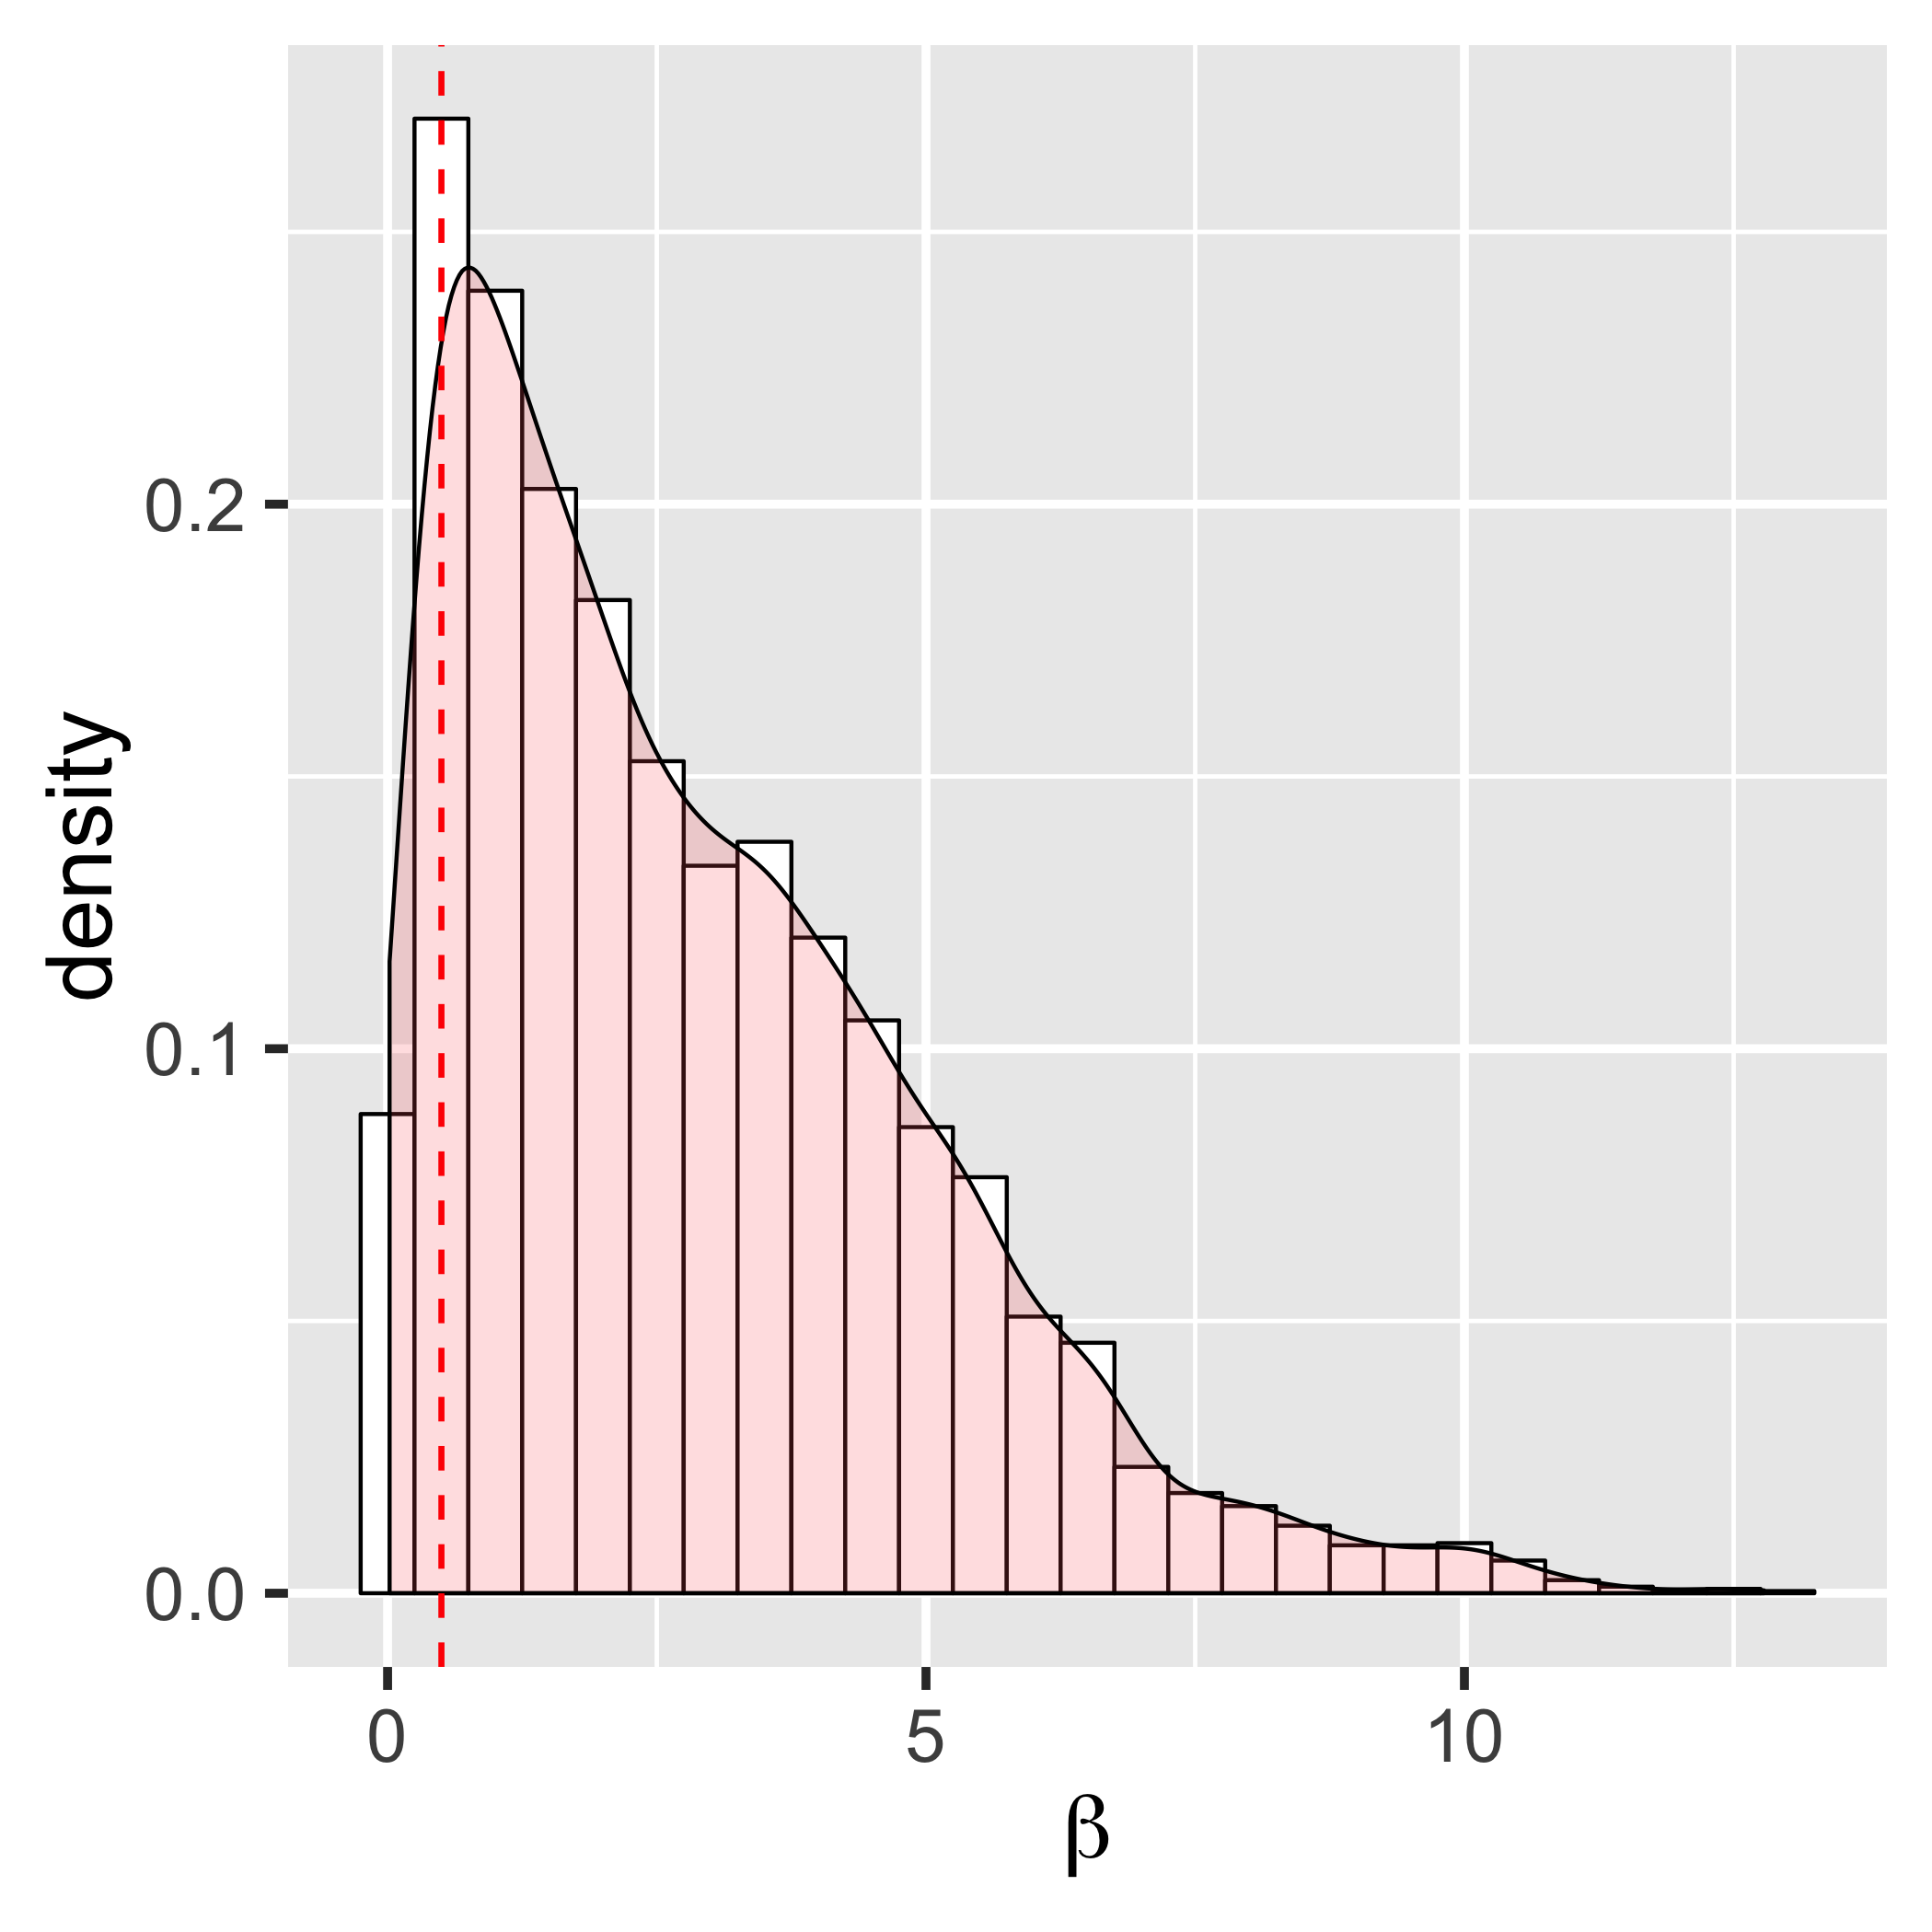
\includegraphics[width=0.5\textwidth]{histogram_Q_beta_posterior.png}}
\vspace{.3in}
\caption{Posterior samples for $\beta$ parameter of Q, red dotted line indicates the ground truth}
\label{fig:beta}
\end{figure}

\begin{figure}[h]
\vspace{.3in}
\centerline{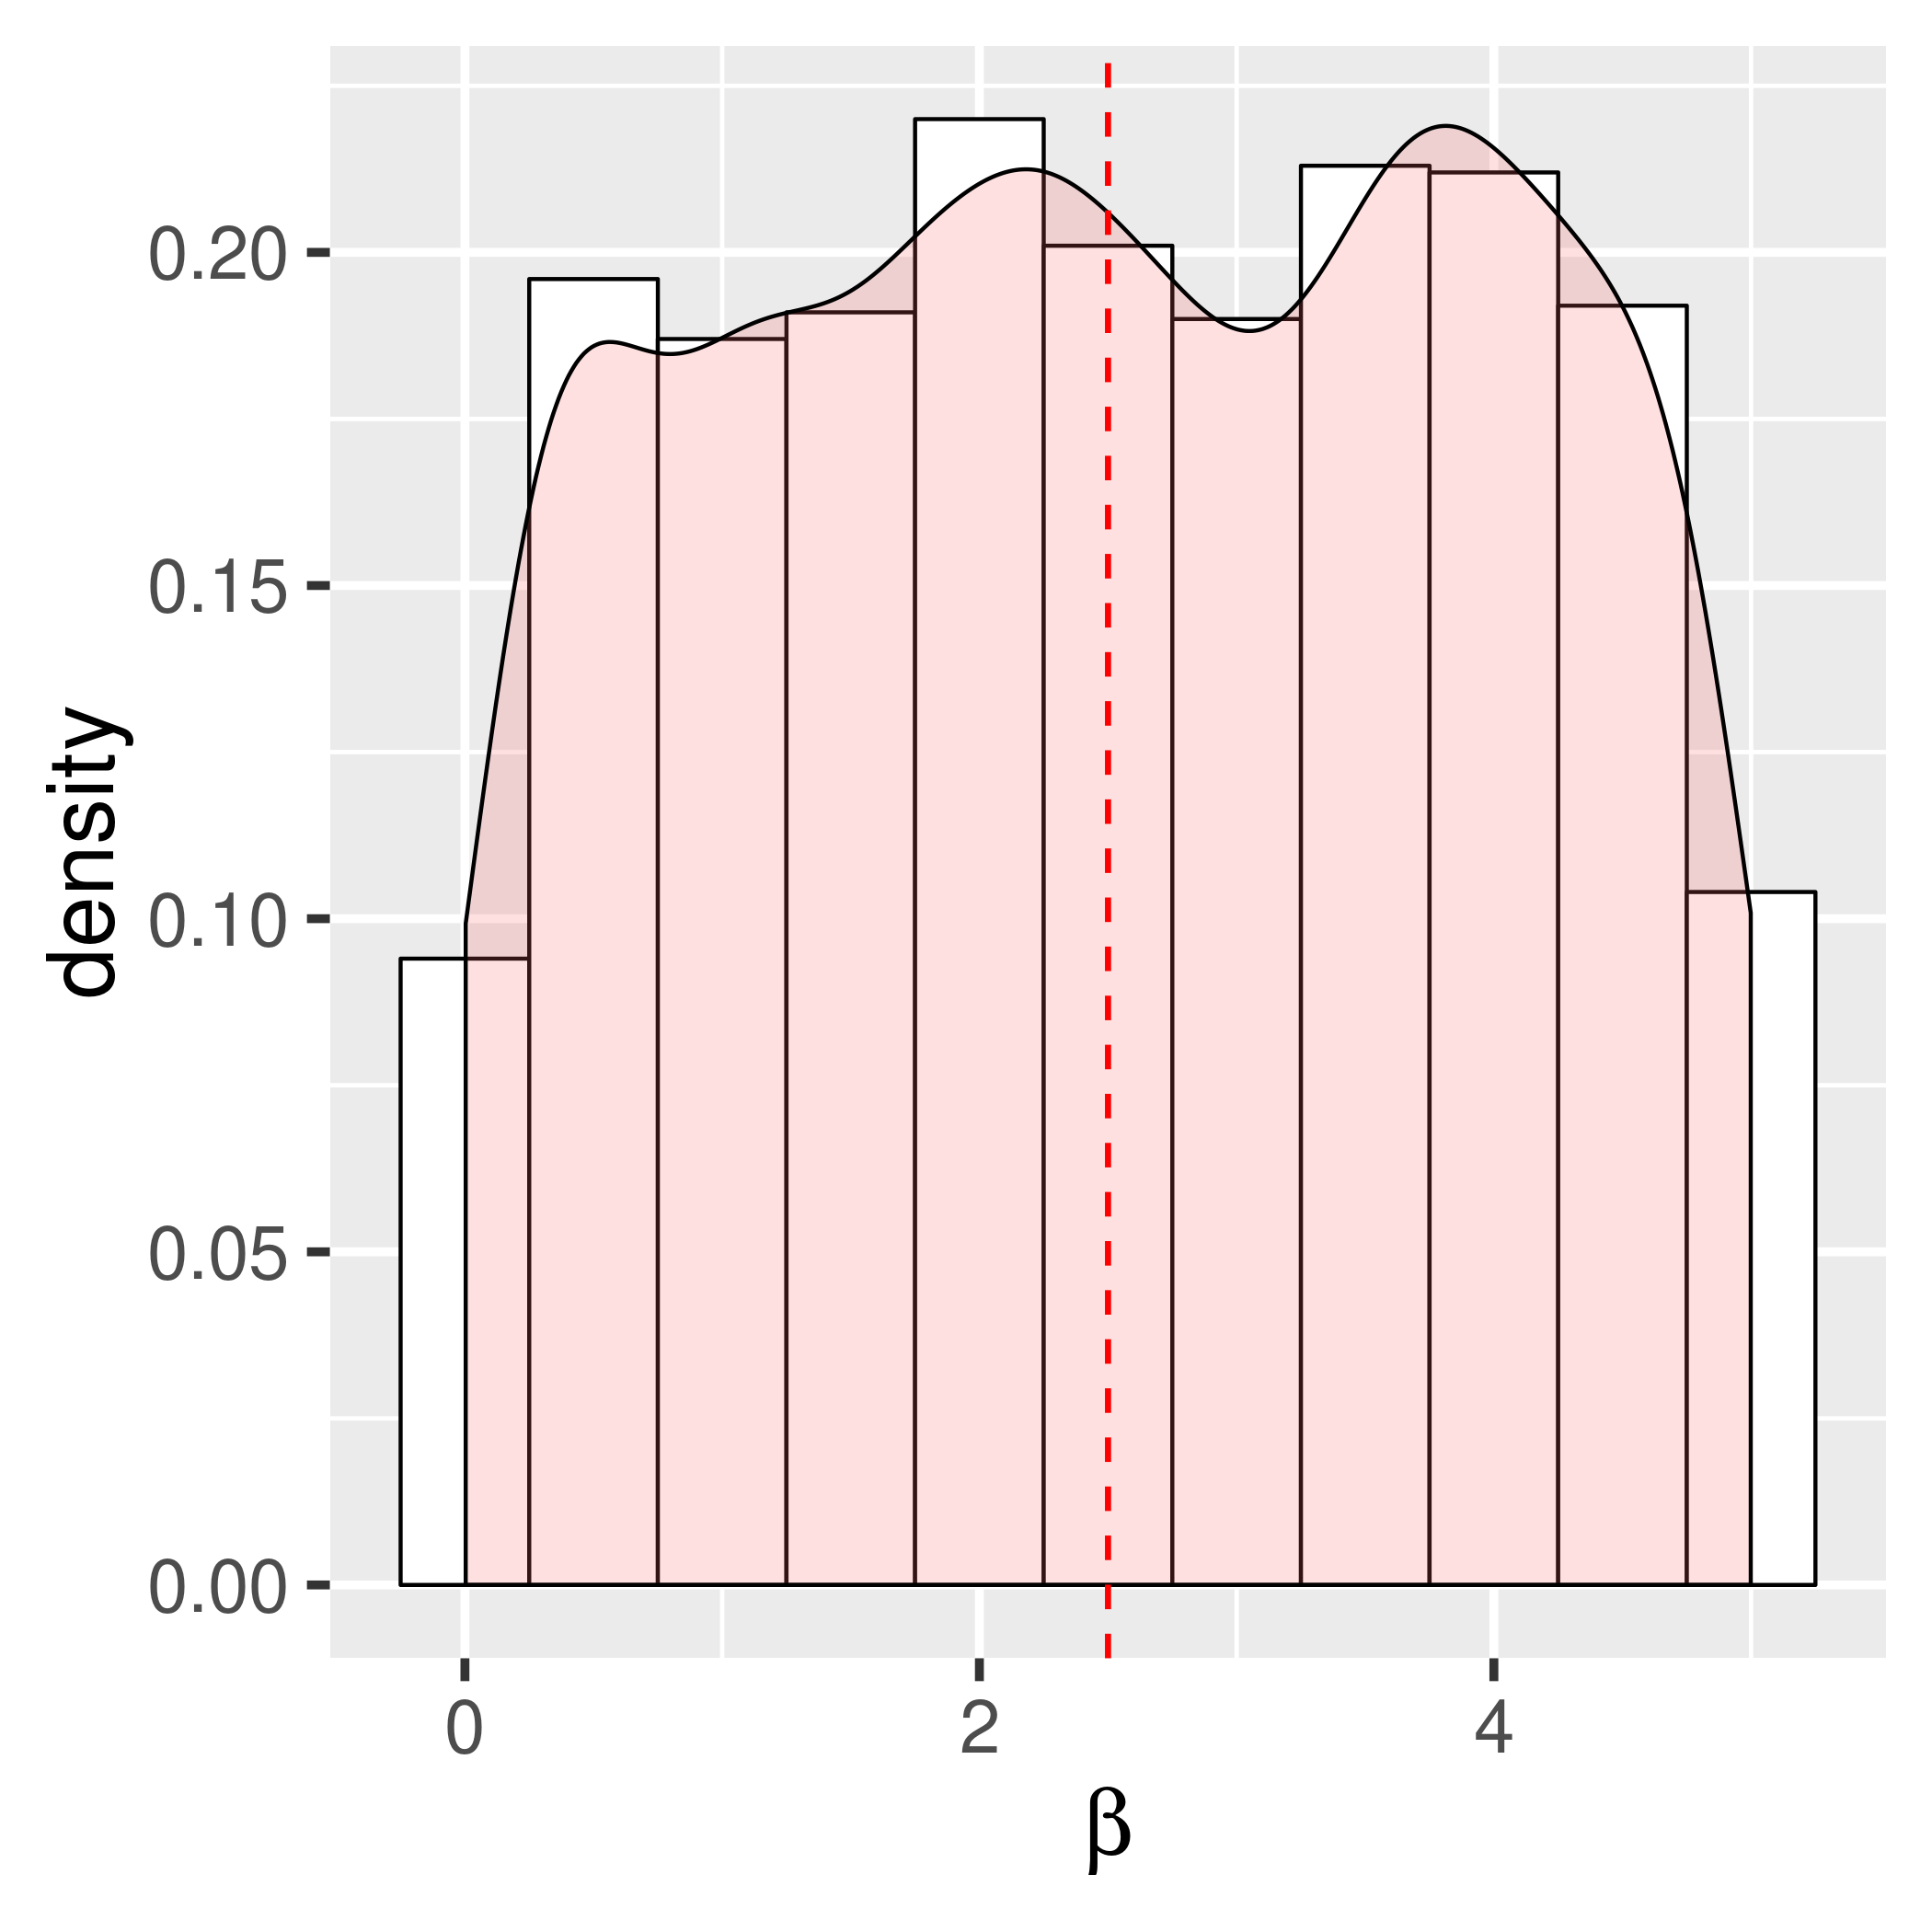
\includegraphics[width=0.5\textwidth]{histogram_Q_beta_prior.png}}
\vspace{.3in}
\caption{Prior samples for $\beta$ parameter of Q, red dotted line indicates the ground truth}
\label{fig:betaprior}
\end{figure}

\begin{figure}[h]
\vspace{.3in}
\centerline{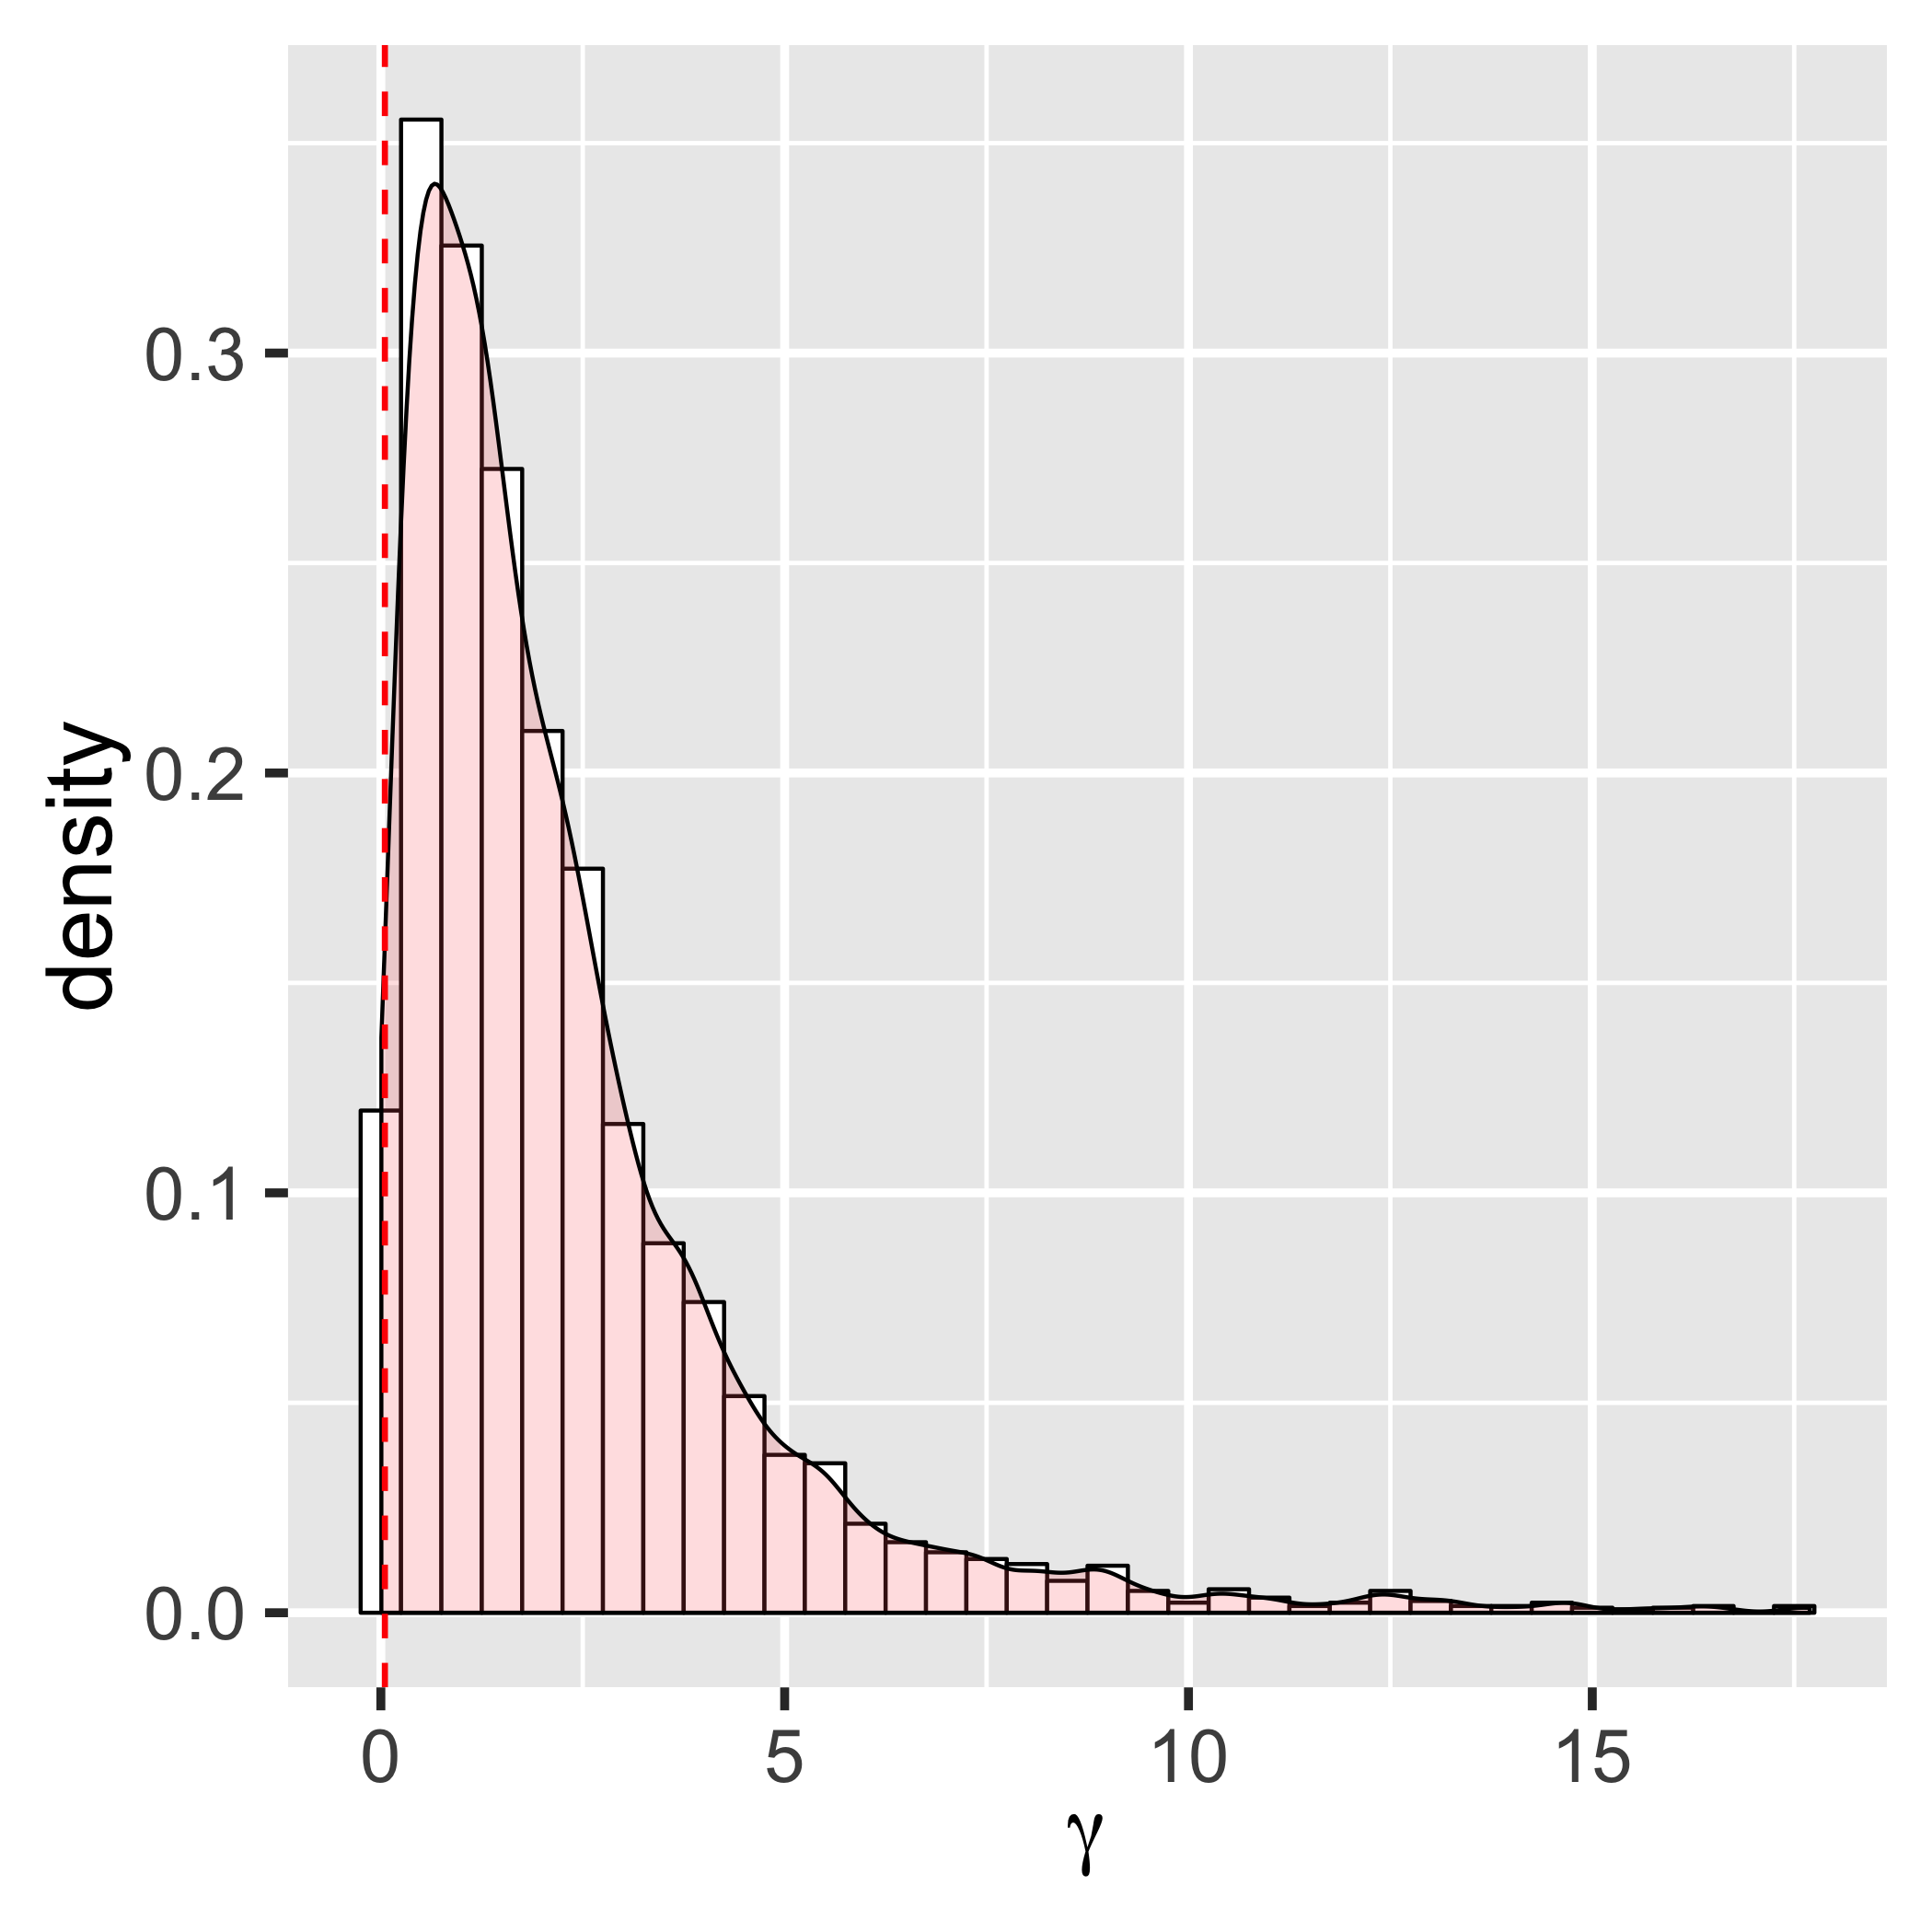
\includegraphics[width=0.5\textwidth]{histogram_Q_gamma_posterior.png}}
\vspace{.3in}
\caption{Posterior samples for $\gamma$ parameter of Q, red dotted line indicates the ground truth}
\label{fig:gamma}
\end{figure}

\begin{figure}[h]
\vspace{.3in}
\centerline{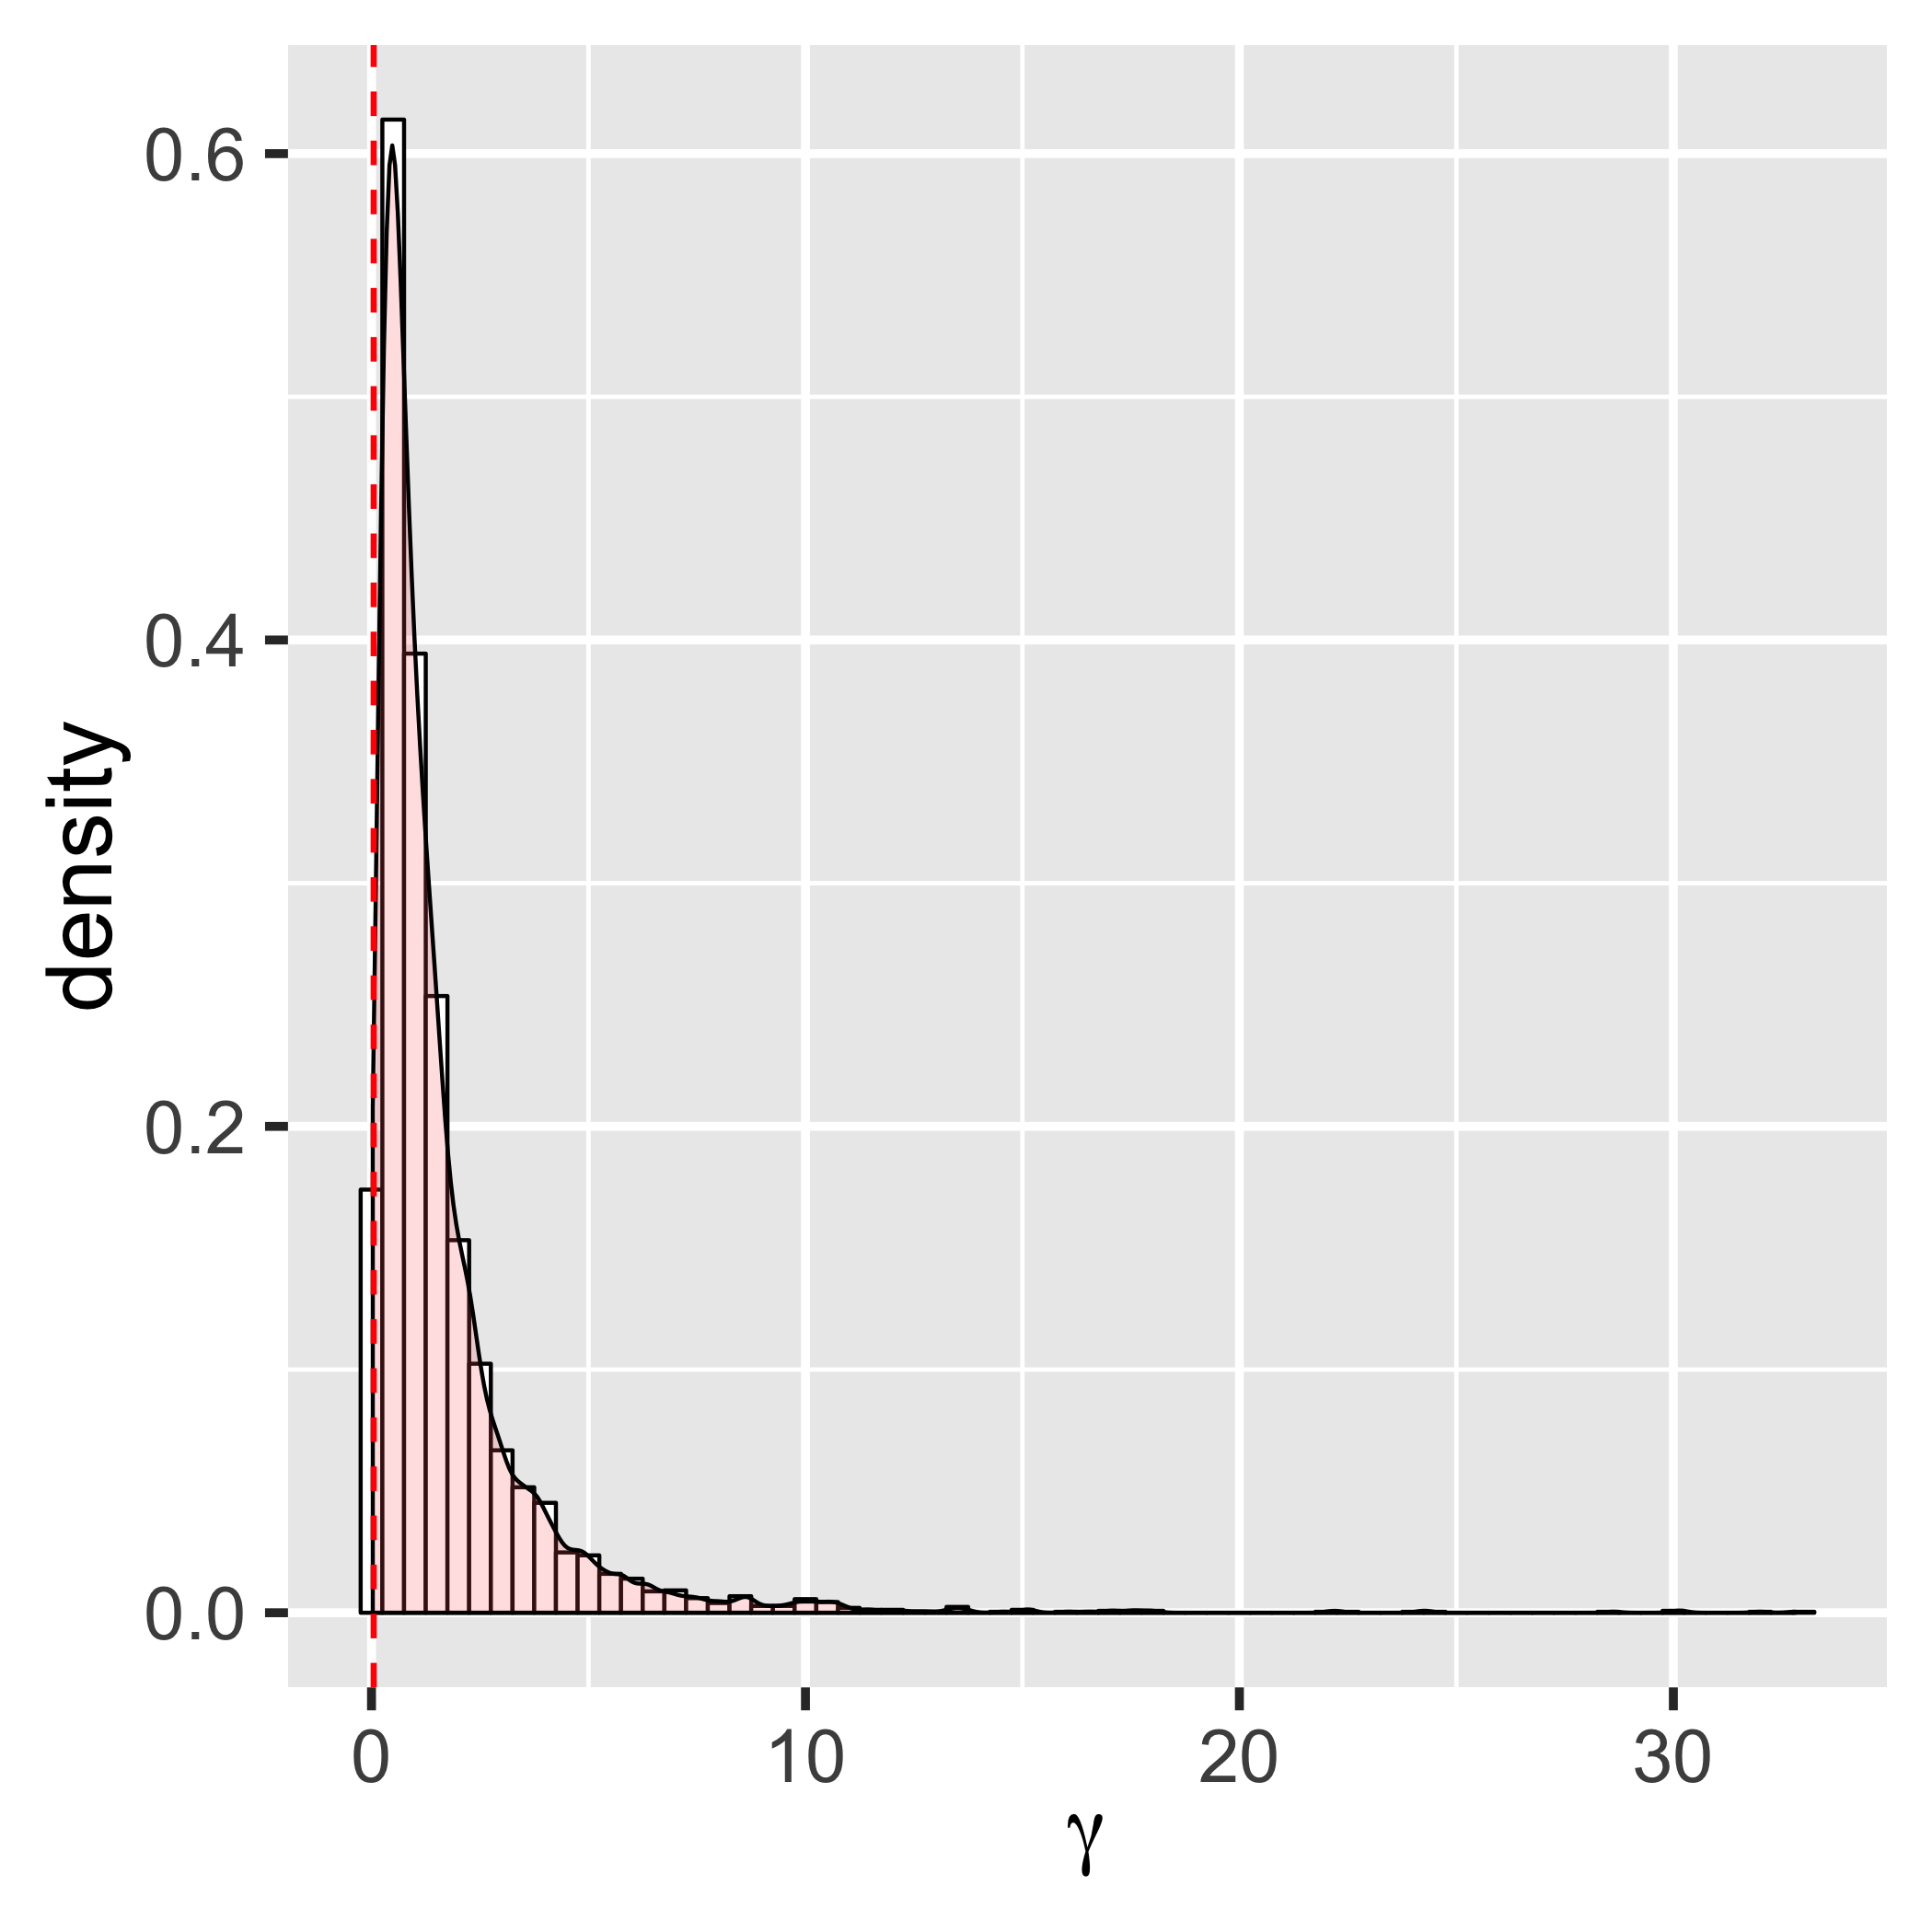
\includegraphics[width=0.5\textwidth]{histogram_Q_gamma_prior.png}}
\vspace{.3in}
\caption{Prior samples for $\gamma$ parameter of Q, red dotted line indicates the ground truth}
\label{fig:gammaprior}
\end{figure}


\begin{figure}[h]
\vspace{.3in}
\centerline{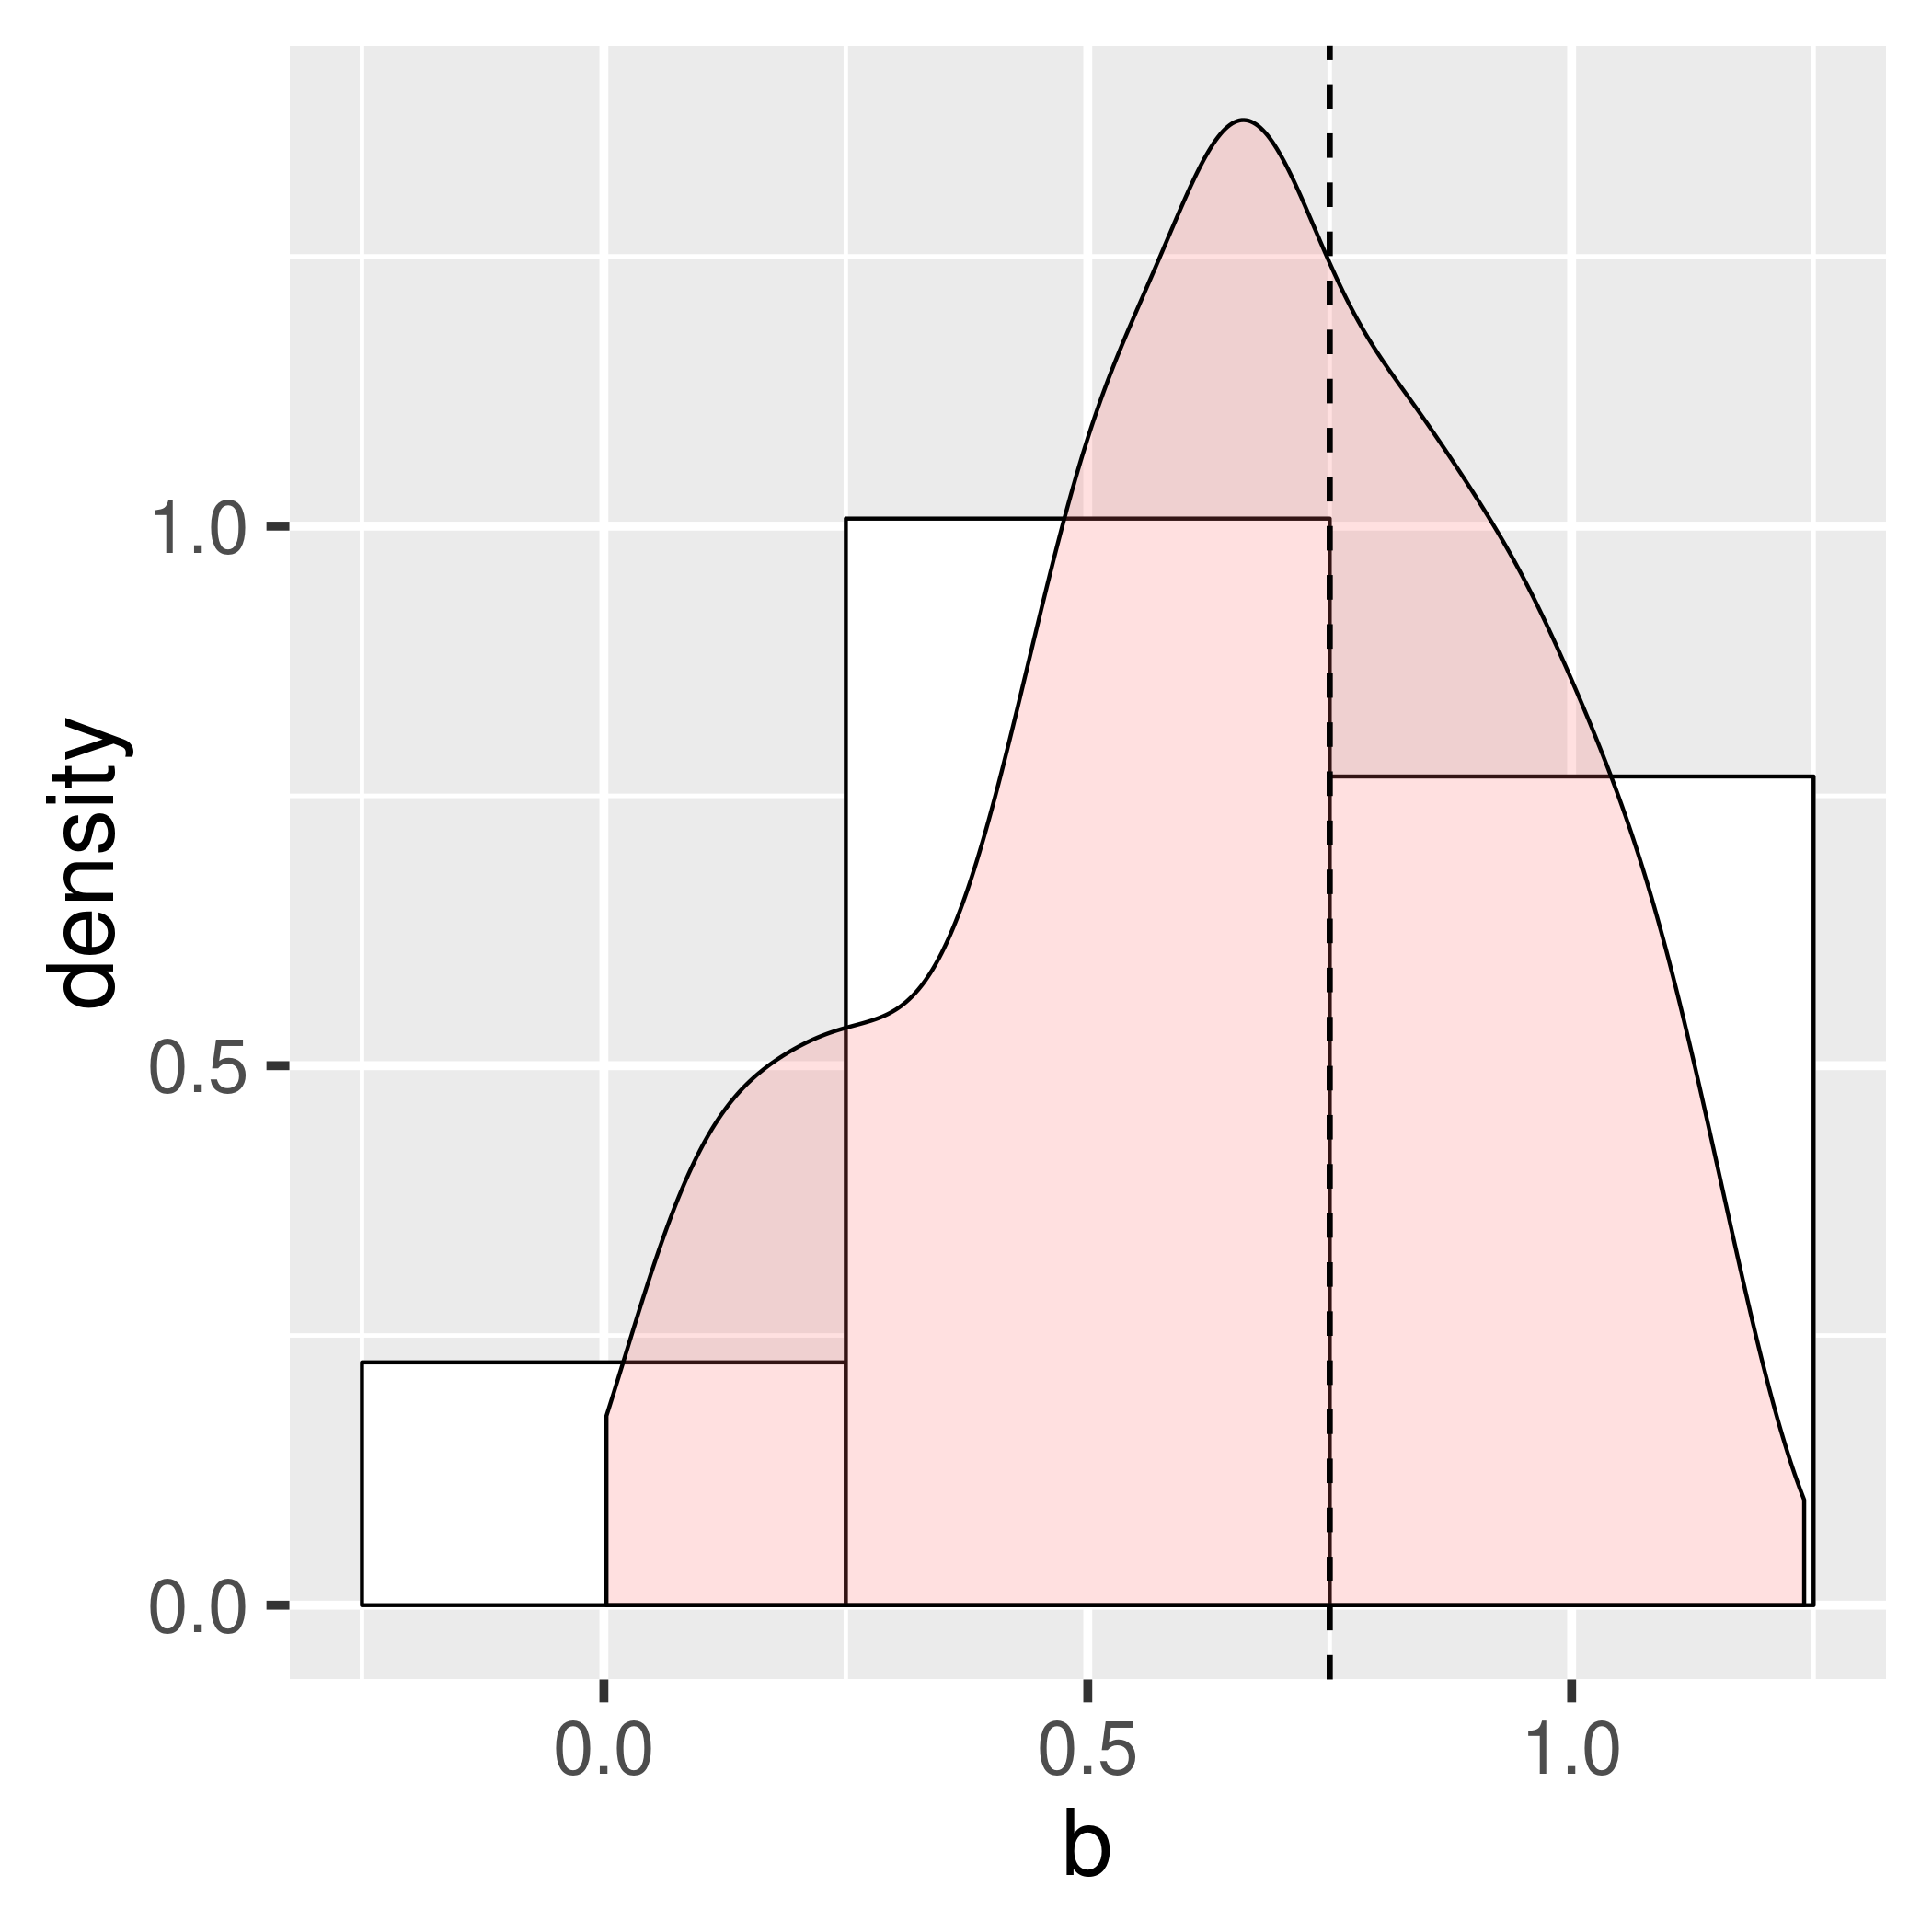
\includegraphics[width=0.5\textwidth]{histogram_Q_b_posterior.png}}
\vspace{.3in}
\caption{Posterior samples for $b$ parameter of Q, red dotted line indicates the ground truth}
\label{fig:b}
\end{figure}

\begin{figure}[h]
\vspace{.3in}
\centerline{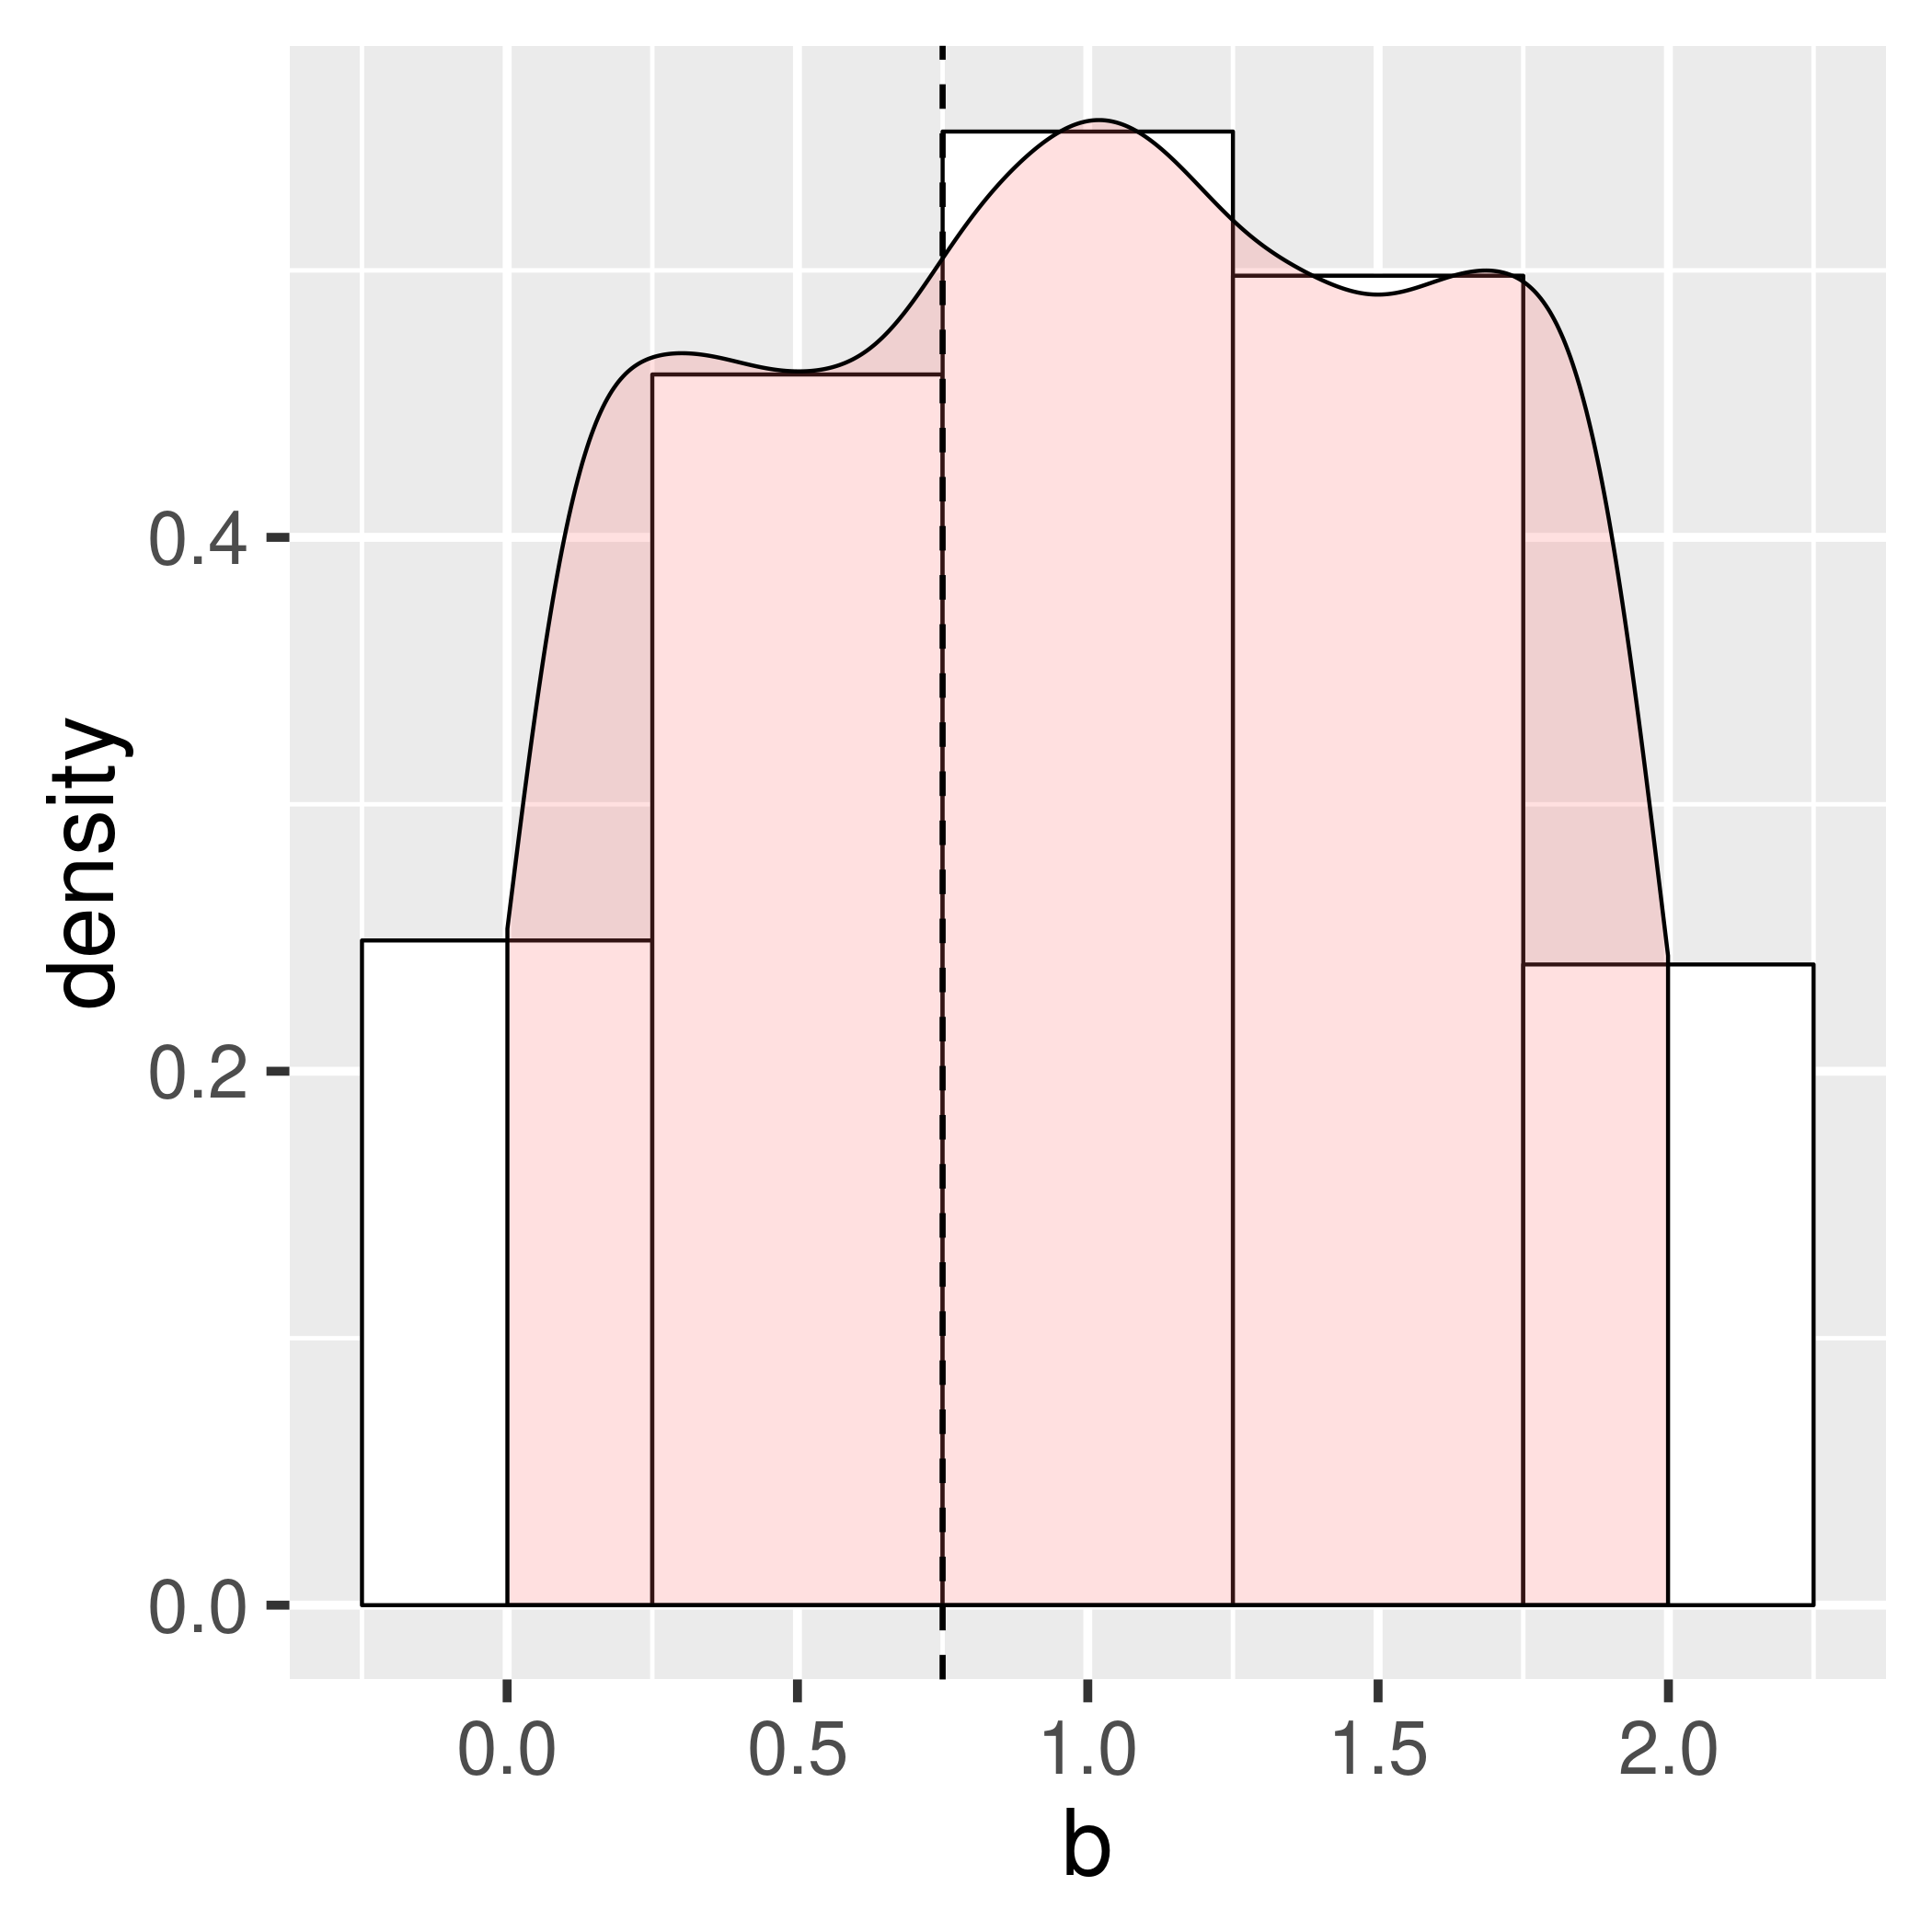
\includegraphics[width=0.5\textwidth]{histogram_Q_b_prior.png}}
\vspace{.3in}
\caption{Prior samples for $b$ parameter of Q, red dotted line indicates the ground truth}
\label{fig:bprior}
\end{figure}

%\bibliographystyle{plainnat}
%\bibliography{references}


\clearemptydoublepage

\chapter{Forecasting Near-Earth Solar Wind Speed: The \XX \ Model}\label{chapter:pdt}

{\small
  We model the joint regression problem where one signal drives another signal with an unknown 
  time delay, with the forecasting of the solar wind speed based on the Sun's magnetic flux, as the 
  motivating application. This problem, called \emph{dynamic time lag regression} (\XX) is 
  formalised using a probabilistic setting, modelling the non-stationary time delay between the 
  causes and the effects on the one hand, and the cause-effect relationship on the other hand. A 
  Bayesian approach is presented to tackle the \XX\ problem together with theoretical 
  justifications based on linear stability analysis. The approach is empirically validated with 
  proofs of concept on synthetic problems and real-world application of near-Earth solar wind speed 
  prediction. 
}


\vfill
\sectionlinetwo{DarkGreen}{88}
\vfill

\noindent
    \parbox{\textwidth}{%
        {\small This chapter is based on research which is under review.}
    }%


\clearpage


\section{Introduction}\label{sec:intro}
A significant body of work in machine learning concerns the modeling of spatiotemporal phenomena 
\citep{SurveyST,NIPSForecasting18}, ranging from markets \citep{Pedreschi} to weather forecasting 
\citep{Horvitz} and space weather prediction \citep{EnricoLorentz,camporeale2018machine,EnricoArxiv}. 
This work focuses on the problem of modeling the temporal dependency between two time series, where 
the latter one is {\em caused} by the former one \citep{Granger} with a non-stationary time delay. 


\subsection{Motivation: Forecasting Near-Earth Solar Wind Speed}\label{sec:motivationsolarwind}
The Sun, a perennial source of charged energetic particles, drives all geomagnetic phenomena within 
the Sun-earth system. Specifically, the Sun ejects charged particles into the surrounding space in 
all directions (solar wind). High speed solar wind is a major threat for the modern world, causing 
severe damage to satellites, telecommunication infrastructure, under sea pipelines, among others. 
\footnote{The adverse impact of space weather is estimated to cost $200$ to $400$ million per year, 
but can sporadically lead to much larger losses.} Interested readers can refer to 
\cref{sec:hmfsolarwind} for some historical background to the modern models of the solar wind and 
the structure Heliospheric Magnetic Field (HMF). 

Forecasting near-Earth solar wind speed (at the $L_1$ point) based on near-Sun data is a problem of 
particular importance in space weather prediction due to its large lead time 
\citep{doi:10.1002/jgra.50429,doi:10.1029/2009SW000542}. The challenge of ambient solar wind 
prediction is two fold. Firstly, although the coronal magnetic field determines the outflow of the 
solar wind, there are no direct measurements of the coronal magnetic field strength. Secondly the 
propagation of the solar wind through the inter-planetary medium introduces a non-stationary time 
delay which currently cannot be directly measured. 

\subsection{State Of The Art}\label{sec:solarwindsota}
Research in solar wind forecasting has generally divided the problem into the following components.
%
\begin{enumerate} 
  \item Using a coronal magnetic field model to extrapolate line of sight photospheric magnetic 
        field measurements, giving an estimation of the coronal magnetic field topology and 
        solar wind flow.
  \item Propagation of the coronal solar wind to $\SI{1}{\astronomicalunit}$ 
        ($\SI{1}{\astronomicalunit}$ is approximately the distance between the Sun and the Earth).
\end{enumerate} 
%
\citet{Reiss_2019} provide an in-depth survey of the state of the art in solar wind prediction, 
they survey the important coronal magnetic field extrapolation models as well as solar wind 
propagation procedures. We provide a quick recap for continuity.

The most commonly used coronal magnetic field extrapolation technique is the Potential Field Source 
Surface model (PFSS) \citep{altschuler1969magnetic,schatten1969model}. The PFSS model assumes a 
current free (potential) magnetic field structure above the photosphere and expresses the magnetic 
field $\mathbf{B}$ as the gradient of a scalar magnetic potential $\mathbf{B} = -\nabla \Psi$ which 
can be solved by constraining the magnetic field to be divergence free ($\nabla^{2}\Psi = 0$). 
Since potential fields give closed magnetic fields, a spherical source surface, where the magnetic 
field is assumed to be radially outwards, is kept as an outer boundary condition. The radius of the 
spherical source surface is generally set to a height of 
$2.5 R_{\odot}$, where $R_{\odot} = \SI{6.957d5}{\kilo\metre}$ is the solar radius. The effects of 
currents have been incorporated in PFSS variants such as the \emph{Potential-Field Current Sheet} 
(PFCS) \citep{schatten1971current} and \emph{Current-Sheet Source Surface} (CSSS) \citep{csss} 
models. 

It is possible to compute from the solutions of PFSS like models, not only the coronal source 
surface magnetic field strength, but also the expansion of the magnetic flux tubes of the HMF; 
the well known \emph{flux-tube expansion} factor ($\mathbf{f}_S$ or FTE). The Wang-Sheeley (WS) 
model \citep{WSAModel} and the improved Wang-Sheeley-Arge (WSA) model 
\citep{arge2000improvement,arge2004stream} both derive empirical relationships between 
$\mathbf{f}_S$ computed from the PFSS technique and the source surface solar wind speed $v_S$.  

After computing the coronal magnetic field topology and the source surface solar wind speed, 
solar wind streams must be propagated to a distance of around $\SI{1}{\astronomicalunit}$ to 
estimate near-Earth solar wind speeds. \citet{Riley2011} provide a survey of various solar wind 
propagation models, in order of increasing computational complexity. 

The simplest propagation technique, known as the \emph{ballistic mapping}, assumes constant 
velocity propagation from the upper corona ($30R_{\odot}$) to the Earth, requiring only a 
longitudinal shift due to solar rotation. \citet{arge2000improvement} proposed the Arge-Pizzo 
kinematic evolution scheme meant to be a middle ground between the ballistic mapping and the more 
complex Magnetohydrodynamics (MHD) models discussed below.

\citet{Riley2011} also propose a solar wind propagation technique known as the 
$1\textrm{-}\text{D}$ Upwind model which uses the inviscid Burger's equation as a simplified model 
of solar wind flow. The source surface solar wind speed $v_S$ can be mapped using the 
$1\textrm{-}\text{D}$ Upwind finite difference scheme to $\SI{1}{\astronomicalunit}$.

The effect of currents is to distort the coronal magnetic field from a current free topology, 
in order to account for the complex dynamics of solar wind flow. PFSS solutions are often used as 
boundary conditions for MHD based simulations of the inner heliosphere 
($20-30 R_{\odot} \ \mathrm{to} \ \SI{1}{\astronomicalunit}$). Common MHD based models include 
\emph{Magnetohydrodynamics Around a Sphere} (MAS) \citep{linker1999magnetohydrodynamic}, ENLIL 
\citep{ODSTRCIL1996,ODSTRCIL1999a,ODSTRCIL1999b,ODSTRCIL2003,ODSTRCIL2004} and EUHFORIA 
\citep{pomoell2018euhforia}. 

The most prominent operational solar wind forecasting technique is the hybrid WSA-ENLIL model 
\footnote{\url{https://www.swpc.noaa.gov/products/wsa-enlil-solar-wind-prediction}} which consists 
of the Wang-Sheeley-Arge (WSA) coronal model coupled with the global heliospheric ENLIL model. 

\citet{wintoft1997prediction} used coronal magnetic field solutions computed by the PFSS model 
to train a \emph{radial basis function} (RBF) network for predicting the average daily solar wind 
speed $3$ days ahead.  

\citet{Owens2017} used the solutions of MAS model simulated until $30R_{\odot}$ to construct an 
ensemble of near-Sun solar wind conditions and forward propagated these conditions to 
$\SI{1}{\astronomicalunit}$ to give probabilistic forecasts of the near-Earth solar wind speed. 
\citet{Owens2019} proposed a variational data assimilation scheme which used the 
$1\textrm{-}\text{D}$ Upwind model and solar wind speed measurements from $L_1$ to improve inner 
boundary conditions at $30R_{\odot}$.

The current crop of solar wind propagation techniques provide several options for 
modelers, but they pose one or two key issues: 
%
\begin{enumerate*} 
  \item they are computationally intensive 
  \item they fail to assimilate and learn from data 
\end{enumerate*}. 
%
In this chapter we propose a novel machine learning technique for forecasting near-Earth solar wind 
speed from the source surface radial magnetic field strength and $\mathbf{f}_S$ computed by the 
CSSS model as well as the sunspot number and the $\mathrm{F}10.7$ radio flux. Our proposed model 
works by constructing a probability distribution over possible time delays between near-Sun 
quantities and near-Earth solar wind observations and then uses the aforementioned probability 
distribution to formulate a weighted regression problem. The forecasts are assumed to be the output 
of a neural network architecture. Below we setup the background of our method in the machine 
learning context.

\subsection{Predicting What \& When}\label{sec:dtlrintro}
Formally the goal is to model the dependency between heliospheric observations, referred to as 
{\em cause series}, and the solar wind speed series recorded at $L_1$, referred to as 
{\em effect series}. The key difficulty is that the time lag between an input and its effect, the 
solar wind speed recorded at $L_1$, varies from about $2$ to $5$ days depending on, among many 
factors, the initial speed of the solar wind and its interplay with the HMF. Would the lag be 
constant, the solar wind prediction problem would boil down to a mainstream regression problem. The 
challenge here is to predict, from solar data $x(t)$ at time $t$ the value $y(t+\tau)$ of the solar 
wind speed reaching the Earth at time $t+\tau$ where both the value $y(t+\tau)$ and the time lag 
$\tau$ depend on $x(t)$.

To our knowledge the regression problem of predicting both {\em what} the effect is and {\em when} 
the effect is observed constitutes a new machine learning problem, that we called 
{\em Dynamic Time-Lag Regression} (\XX). Indeed, the modeling of dependencies among financial time 
series has been intensively tackled \citep{ZHOU2006195}. When considering varying time lag, many 
approaches rely on dynamic time warping (DTW) \citep{SakoeShiba1978}. For instance, DTW is used in 
\citet{SignalDiffusion}, taking a Bayesian approach to achieve the temporal alignment of both 
series under some restricting assumptions (considering slowly varying time lags and linear 
relationships between the cause and effect time series). More generally, the use of DTW in time 
series analysis relies on simplifying assumptions on the cause and effect series 
(same dimensionality and structure) and build upon available cost matrices for the temporal 
alignment. 

This study focuses on the \XX\ regression problem and the identification of varying time-lag 
phenomena involving stochastic dependencies of arbitrary complexity. The originality of the 
proposed approach compared to the state of the art in DTW series alignment is threefold. Firstly, 
the cause and effect series are of different dimensionality. While the effect series is scalar, the 
cause series can be high-dimensional (e.g. images, vectors, etc). Secondly, the relationship 
between the cause and the effect series can be non-linear (the {\em what} model). Thirdly, the time 
lag phenomenon (the {\em when} model) can be non smooth (as opposed to e.g. \citet{ZHOU2006195}).

The Bayesian approach proposed to tackle the \XX\ regression problem and the associated learning 
equations are described in \cref{sec:dtlrformulation}, followed by a stability analysis and 
a proof of consistency (\cref{sec:dtlrtheory}). The algorithm is detailed in section 
\ref{sec:model}. The experimental setting used to validate the approach is presented in section 
\ref{sec:pdtExp}, and the proofs of concept of the approach are discussed in section 
\ref{sec:proofconcept}

\paragraph{Notations}
Given two time series, the cause series $x(t)$ and the observed effect series $y(t)$, the sought 
model consists of a mapping $f(.)$ which maps each input pattern $x(t)$ to an output $y(t')$, and a 
mapping $g(.)$ which maps $x(t)$ onto the time delay $t'-t$ between the input and output patterns:
%
\begin{align}
y(t + \tau(t)) & = f[x(t)]\label{eq:pb1}\\
\tau(t) & = g[x(t)]\label{eq:pb2} 
\end{align}
with
\[
f: \mathcal{X}  \rightarrow \mathbb{R},\qquad\text{and}\qquad
g: \mathcal{X}  \rightarrow \mathbb{R}^{+},
\]
where $t \in \mathbb{R}^{+}$ represents the continuous temporal domain. The input signal 
$x(t)\in \mathcal{X}$ is possibly high dimensional and contains the hidden cause to 
the effect $y(t)\in\mathbb{R}$ which is considered as a scalar in this chapter. 
$\tau(t)\in \mathbb{R}^+$ represents the time delay between inputs and outputs.
Vectors are written using bold fonts.

\section{Probabilistic Dynamically Delayed Regression}\label{sec:dtlrformulation}
As said, \cref{eq:pb1,eq:pb2} define a regression problem that differs from standard regression 
along two lines. Firstly, the time lag $\tau(t)$ is non-stationary as it depends on $x(t)$. 
Secondly, $\tau(t)$ is unknown, i.e. it is not recorded explicitly in the training data as is 
typically the case in the space weather context. 

\subsection{Assumptions}

For the sake of the model identifiability and computational stability, the delay function 
$\phi(t) = t + \tau(t)$ is assumed to be sufficiently regular w.r.t. $t$. Formally, $\phi(.)$ 
is assumed to be continuous.

For some authors \citep{ZHOU2006195} the monotonicity of $\phi(.)$ is additionally required and 
enforced using constraints: $\phi(t_1) \leq \phi(t_2), \forall t_1 \leq t_2$. However, this 
assumption will not be retained in the following as it does not hold in the space weather domain 
(e.g. fast moving solar wind can reach the Earth before slow moving solar wind which departed 
before it). 

\subsection{Probabilistic Dynamic Time-Lag Regression}

For practical reasons, cause and effect series are sampled with a constant rate $\delta t$, and 
respectively noted ${x_m}$ and ${y_m}$ in the following. Accordingly, mapping $g$ might be sought 
as a discrete time lag, where the delay between cause $x_m$ and effect $y_{m+g(x_m)}$ ranges in a 
finite set $T = [\tau_{min}, \ldots, \tau_{max}]$, with  $\tau_{min}$ and  $\tau_{max}$ defined 
from prior knowledge, e.g. space weather theory. 

The unavoidable error due to the discretization of the continuous time lag is mitigated along a 
probabilistic model, associating to each cause $x$, a set of independent predictors 
$\{\hat y_i(x),\ i \in T\}$ and a probability distribution $\hat p(x)$ on $T$ estimating the 
probability of delay of the effects of $x$. Overall, the \XX\ solution is sought as a probability 
distribution conditioned on cause $x$, mixture of Gaussians centered on the predictors 
$\hat y_i(x)$, where the mixture weights are defined from $\hat p(x)$. More formally, letting 
${\bf y}_m$ denote the vector of random variables $y_{m+i},\ i \in T$, 
%
\begin{equation}\label{eq:py}
  P\bigl[{\bf y}_{m}\vert x_m=x\bigr] = 
  \sum_{i \in T, \tau_i\in\{0,1\}} \hat p\bigl(\tau_1,\ldots,\tau_n\vert x) 
  \prod_{i\in T} {\cal N}\bigl(\hat y_i(x),\sigma_i(\tau)\bigr)
\end{equation}
%
Two simplifications are made for the sake of the analysis. Firstly, the stochastic time lag is 
modelled as the set $\{\tau_i, i \in T\}$ of binary latent variables, where $\tau_i$ indicates 
whether $x$ drives $y_i$ ($\tau_i=1$) or not ($\tau_i=0$). The assumption that every cause has a 
single effect is modelled by imposing: \footnote{Note however that the cause-effect correspondence 
might be many-to-one, with an effect depending on several causes.}
%
\begin{equation}\label{eq:cs1}
\sum_{i \in T} \tau_i = 1.
\end{equation}
%
From constraint~\cref{eq:cs1}, probability distribution $\hat p(x)$ thus is sought as a set of 
$\hat p_i(x)$ for $i$ in $T$, summing to 1, such that $\hat p_i(x)$ stands for the probability of 
the effect of $x_m=x$ to occur with delay $i$ in $T$.

The second simplifying assumption is that the variance $\sigma_i^2({\bf \tau})$ of predictor 
$\hat h_i$ does not depend on $x$, by setting:
\[
\sigma_i({\bf \tau})^{-2} = \Bigl(1+\sum_j\alpha_{ij} \tau_j\Bigr)\sigma^{-2},
\]
with $\sigma^2$ a default variance and $\alpha_{ij}\ge 0$ a matrix of non-negative real parameters. 
The fact that $x$ can influence $y_i$ through predictor $\hat y_i(x)$ even when $\tau_i=0$ reflects 
an indirect influence due to the auto-correlation of the $y$ series. This influence comes with a 
higher variance, enforced by making $\alpha_{ij}$ a decreasing function of $\vert i-j\vert$. More 
generally, a large value of $\alpha_{ii}$ compared to $\alpha_{ij}$ for $i\ne j$ corresponds to a 
small auto-correlation time of the effect series. 

\subsection{Learning Criterion}
The joint distribution is classically learned by maximizing the log likelihood of the data, that 
can be computed in closed form as (please see \cref{app:LL} for the details of the derivation): 
%
\begin{equation}\label{eq:LL}
  {\cal L}\bigl[ {\bf x, y};\hat {\bf y},\hp,\sigma,{\bf \alpha}] = 
  -\vert T\vert\log(\sigma)-\frac{1}{n_m}\sum_m\Bigl[
    \sum_{i \in T}\frac{1}{2\sigma^2}\bigl(y_{m+i}-\hat y_i(x_m)\bigr)^2 - 
    \log\bigl(Z_m(\hat {\bf y},\hp,\sigma,{\bf \alpha})\bigr)\Bigr],
\end{equation}
%
with $n_m$ the number of data points and partition term $Z_m$ given as:
\[
  Z_m(\hat {\bf y},\hp,\sigma,{\bf \alpha}) = \sum_{i \in T}\hat p_i(x_m)\exp\Bigl(
    - \frac{1}{2\sigma^2}\sum_{j\in T}\alpha_{ji}\bigl(y_{m+j}-\hat y_j(x_m)\bigr)^2 
    + \frac{1}{2}\sum_{j\in T}\log(1+\alpha_{ji})\Bigr).
\]
For notational simplicity, the data index $m$ is omitted in the following and the empirical 
averaging on the data is noted ${\mathbb E}_{data}$. The hyper-parameters $\sigma$ and matrix 
$\alpha$ of the model are obtained by optimizing  ${\cal L}$:
%
\begin{equation}\label{eq:var}
  \frac{\sigma^2}{1+\alpha_{ij}} = 
  \frac{
    {\mathbb E}_{data}\bigl[\bigl(y_i-\hat y_i(x)\bigr)^2q_j(x,{\bf y})\bigr]
  }{
    {\mathbb E}_{data}\bigl[q_j(x,{\bf y})\bigr]
  },
\end{equation}
%
with the probability $q_i(x,{\bf y}) = P(\tau_i=1\vert x,{\bf y})$ defined as
%
\begin{equation}\label{eq:hatpi}
  q_i(x,{\bf y}) = \frac{1}{
    Z(\hat {\bf y},\hp,\sigma,{\bf \alpha})
  } \hat p_i(x) 
  \exp\Bigl(
    - \frac{1}{2\sigma^2}\sum_{j\in T}\alpha_{ji}\bigl(y_j-\hat y_j(x)\bigr)^2 
    + \frac{1}{2}\sum_{j\in T}\log(1+\alpha_{ji})
  \Bigr)
\end{equation}
%
In addition the optimal $\hat {\bf y}$ and $\hp$ reads:
%
\begin{align}
  \hat y_i(x) &= 
    \frac{
      {\mathbb E}_{data} \Bigl[
          y_i\bigl(1+\sum_{j\in T}\alpha_{ij}q_j(x,{\bf y})\bigr)\Big\vert x
        \Bigr]
    }{
      {\mathbb E}_{data}\Bigl[1+\sum_{j\in T}\alpha_{ij}q_j(x,{\bf y})\Big\vert x\Bigr]
    }\label{eq:hyopt}\\[0.2cm]
  \hat p_i(x) &= {\mathbb E}_{data}\Bigl[q_i(x,{\bf y})\Big\vert x \Bigr],\label{eq:tildep}
\end{align}
%
where the above conditional empirical averaging operates as an averaging over samples close to $x$.

These are implicit equations, since $q_i(x,{\bf y})$ depends on the parameters $\sigma^2$ and 
$\alpha_{ij}$, $\hat {\bf y}$ and $\hp$. The proposed algorithm detailed in \cref{sec:model} 
implements the saddle point method defined from \cref{eq:var,eq:hatpi,eq:hyopt,eq:tildep}: 
alternatively, hyper-parameters $\sigma$ and $\alpha_{ij}$ are updated from \cref{eq:var} based on 
the current $\hat y_i$ and $\hat p_i$; and predictors $\hat y_i$ and mixture weights $\hat p_i$ are 
accordingly updated from \cref{eq:hyopt} and \cref{eq:tildep} respectively. 

\section{Theoretical Analysis}\label{sec:dtlrtheory}
The proposed \XX\ approach is shown to be consistent and analysed in the simple case where $\alpha$ 
is a diagonal matrix ($\alpha_{ij} = \alpha\delta_{ij}$).

\subsection{Loss Function \& Optimal Predictor}\label{sec:prop}
Let us assume that the hyper-parameters of the model have been identified together with predictors 
$\hat y_i(x)$ and weights $\hat p_i(x)$. These are leveraged to achieve the prediction of the 
effect series. For any given input $x$, the sought eventual predictor is expressed as 
$(\hat y(x),\hat I(x))$ where $\hat I(x)$ is the predicted time lag and $\hat y(x)$ the predicted 
value. The associated $L_2$ loss is: 
%
\begin{equation}\label{eq:orloss}
  {\cal L}_2(\hat y,\hat I) = {\mathbb E}_{data}\Bigl[\bigl(y_{\hat I(x)}-\hat y(x)\bigr)^2\Bigr]. 
\end{equation}
%
Then it follows:
%
\begin{prop}\label{prop:opred}
with same notations as in \cref{eq:py}, with $\alpha_{ij} = \alpha\delta_{ij},\ \alpha>0$, 
the optimal composite predictor $(y^\star,I^\star)$ is given by
\[
  y^\star(x) = 
    \hat y_{I^\star(x)}(x)\qquad\text{with}\qquad I^\star(x) = \argmax_{i} \bigl(\hat p_i(x)\bigr), 
\]
\end{prop}
%
\begin{proof}
In \cref{app:Hessian}.
\end{proof}

\subsection{Linear Stability Analysis}\label{sec:stability}
The saddle point \cref{eq:var,eq:hatpi,eq:hyopt,eq:tildep} admit among others a degenerate 
solution $\mathbf{p}_0$ corresponding to $\hat p_i(x) = 1/\vert T\vert$, 
$\alpha_{ij}=0, \forall i,j \in T$, with $\sigma^2 = \sigma_0^2$. Informally the model converges 
toward this degenerate trivial solution when there is not enough information to build specialised 
predictors $\hat y_i$. 

Let us denote $\Delta y_i^2(x)= \bigl(y_i-\hat y_i(x)\bigr)^2$ the square error made by predictor 
$\hat y_i$ for $x$, and 
\[
  \sigma_0^2 = \frac{1}{|T|}{\mathbb E}_{data}\Bigl(\sum_{i \in T } \Delta y_i^2(x)\Bigr)
\]
the MSE over the set of the predictors $\hat y_i$, $i \in T$. 

Let us investigate the conditions under which the degenerate solution may appear, by computing the 
Hessian of the log-likelihood and its eigenvalues. Under the simplifying assumption
\[
  \alpha_{ij} = \alpha \delta_{ij},
\]
the model involves $2\vert T\vert+2$ parameters: $\alpha$, $r = \sigma^2/\sigma_0^2$, 
$\hat {\bf y}$ and $\hp$. After the computation of the Hessian (\cref{app:opred}) the system 
involves three key statistical quantities, two global:
%
\begin{align}
  C_1[\p] &= \frac{1}{\sigma_0^2}{
    \mathbb E}_{data}
      \Bigl(
        \sum_{i \in T} q_i(x,{\bf y})\Delta y_i^2(x)
      \Bigr), \label{def:C1}\\[0.2cm]
  C_2[\p] &= \frac{1}{\sigma_0^4} {\mathbb E}_{data} 
    \Bigl[\sum_{i\in T}q_i(x,{\bf y})
      \Bigl(
        \Delta y_i^2(x)-\sum_{j \in T} q_j(x,{\bf y})\Delta y_j^2(x)
      \Bigr)^2
    \Bigr],\label{def:C2}
\end{align}
%
and a one local:
\begin{equation}
  \vert {\bf u}(x)\vert^2 = \sum_{i\in T} C_{2+i}[x,\p]^2,
\end{equation}
%
where ${\bf u}(x)$ is a $\vert T\vert$-vector of components 
%
\[
  C_{2+i}[x,\p] = \frac{1}{\sigma_0^2}{\mathbb E}_{data}
    \Bigl[ q_i(x,{\bf y})
      \bigl(
        \Delta y_i^2(x)-\sum_{j \in T} q_j(x,{\bf y})\Delta y_j^2(x)
      \bigr)\Big\vert x 
    \Bigr].
\]
%
$C_1$ represents the covariance between the latent variables $\{\tau_i\}$ and the normalised 
predictor errors, up to a constant. $C_1 < 1$ indicates a positive correlation between the latent 
variables and small errors; the smaller the better. For the degenerate solution, i.e. 
$\p=\p_{0}$ uniform, $C_1[\p_{0}]=1$ and $C_2[\p_{0}]$ represents the default variability among the 
prediction errors. $C_{2+i}[x,\p]$ informally measures the quality of predictor $\hat y_i$ 
relatively to the other ones. More precisely, a negative value of  $C_{2+i}[x,\p]$ indicates 
that $\hat y_i$ is doing better than average in the neighborhood of $x$.  
%
At a saddle point the parameters are given by:
%
\[
  \frac{\sigma^2}{\sigma_0^2} = 
    \frac{\vert T\vert-C_1[\p]}{\vert T\vert-1} 
    \qquad\text{and}\qquad
    \alpha = \frac{\vert T\vert}{\vert T\vert-1}\frac{1-C_1[\p]}{C_1[\p]}.
\]
%
The predictors $\hat {\bf y}$ are decoupled from the rest whenever they are centered, which we 
assume. If $\hat {\bf p}$ is fixed, a saddle point is stable if and only if
%
\[
  C_2[\p] < 2C_1^2[\p]+{\cal O}\bigl(\frac{1}{\vert T\vert}\bigr).
\]
%
In particular, the degenerate solution is unstable if
%
\[
  C_2[\p_0] > 2\bigl(1-\frac{1}{\vert T\vert}\bigr).
\]
%
Note that when $\Delta y_i(x)$ is i.i.d and centered, with variance $\sigma_0^2$ and relative 
kurtosis $\kappa$ (conditionally to $x$) one has $C_2 = (2+\kappa)(1-1/\vert T\vert)$. Therefore, 
whenever $\Delta y_i^2(x)$ fluctuates and the relative kurtosis is non-negative,
the degenerate solution is unstable and will thus be avoided.

If $\hat {\bf p}$ is allowed to evolve (after \cref{eq:tildep}), the degenerate trivial 
solution becomes unstable as soon as $\vert {\bf u}(x)\vert^2$ is non-zero, due to the fact that 
the gradient is inversely proportional to ${\bf u}(x)$ (with 
$d\hp(x)\propto -\vert {\bf u}(x)\vert^2 {\bf u}(x)$), thus rewarding the predictors with lowest 
errors by increasing their weights. The system is then driven toward other solutions, among which 
the localised solutions of the form:
% 
\[
  \hat p_i(x) = \delta_{iI(x)},
\]
%
with an input dependent index $I(x)\in T$. As shown in \cref{app:Hessian}, the solution of highest 
likelihood of this type is also optimal with respect to the loss function~(\cref{eq:orloss}). The 
stability of such localised solutions and the existence of other (non-localised) solutions is left 
for further work.  


\section{Overview Of The \XX\ Algorithm}\label{sec:model}
\begin{algorithm}[H]
  \SetAlgoLined
   \caption{\XX\ algorithm}
   Initialization of $\alpha$ and $\sigma$\\
   $it \longleftarrow 0$ \;
   \While{it $<$ max}{
    \While{epoch}{
      $\theta \longleftarrow Optimise(\mathcal{L}(\theta, \alpha, \sigma^2))$ \;
    }
    $\sigma^2 \longleftarrow \sigma_0^2 \frac{\vert T\vert-C_1[\p]}{\vert T\vert-1}$ \;
    $\alpha \longleftarrow \frac{\vert T\vert}{\vert T\vert-1}\frac{1-C_1[\p]}{C_1[\p]}$ \;
   }
  \KwResult{Model parameters $\theta$, hyper-parameters $\alpha, \sigma^2$}
\end{algorithm}
The \XX\ algorithm learns both regression models $\hat {\bf y}(x)$ and $\hat {\bf p}(x)$ from 
series $x_m$ and $y_m$, using alternate optimization of the model parameters and the model 
hyper-parameters ${\bf \alpha}$ and $\sigma^2$, after \cref{eq:var,eq:hatpi,eq:hyopt,eq:tildep}. 
The model search space is that of neural nets, parametrized by their weight vector $\theta$. 
The inner optimization loop updates $\theta$ using mini-batch based stochastic gradient descent. 
At the end of each epoch, after all mini-batches have been considered, the outer optimization loop 
computes hyper-parameters ${\bf \alpha}$ and $\sigma^2$ on the whole data. 
 
The initialization of hyper-parameters $\alpha$ and $\sigma$ is settled using preliminary 
experiments (same setting for all considered problems: 
$\alpha \sim U(0.75, 2)$; $\sigma^2 \sim U(10^{-5}, 5)$).

The neural architecture implements predictors $\hat {\bf y}(x)$ and weights $\hat {\bf p}(x)$ on 
the top of a same feature extractor from input $x$. The architecture of the feature extractor is a 
two-hidden layer fully connected network. On the top of the feature extractor are the 
one-layer $\hat {\bf y}$ and $\hat {\bf p}$ models, each with $|T|$ output neurons, with $|T|$ the 
size of the chosen interval for the time lag.

\begin{table}[htbp]
  \caption{Network Architecture Details}\label{tab:arch_probs}
  \centering
  \begin{tabular}{ r c c c }
  \hline
  Problem &  \# Hidden layers & Layer sizes & Activations\\
  \hline
  \textbf{I} & $2$ & $[40, 40]$  & [ReLU, Sigmoid]\\
  \textbf{II} & $2$ & $[40, 40]$ & [ReLU, Sigmoid]\\
  \textbf{III} & $2$ & $[40, 40]$ & [ReLU, Sigmoid]\\
  \textbf{IV} & $2$ & $[60, 40]$ & [ReLU, Sigmoid]\\
  \textbf{Solar Wind} & $2$ & $[60, 80]$ & [ReLU, Sigmoid]\\
  \hline
  \end{tabular}
\end{table}


\begin{figure}[ht]
\centerline{\resizebox*{0.7\textwidth}{!}{\begin{picture}(0,0)%
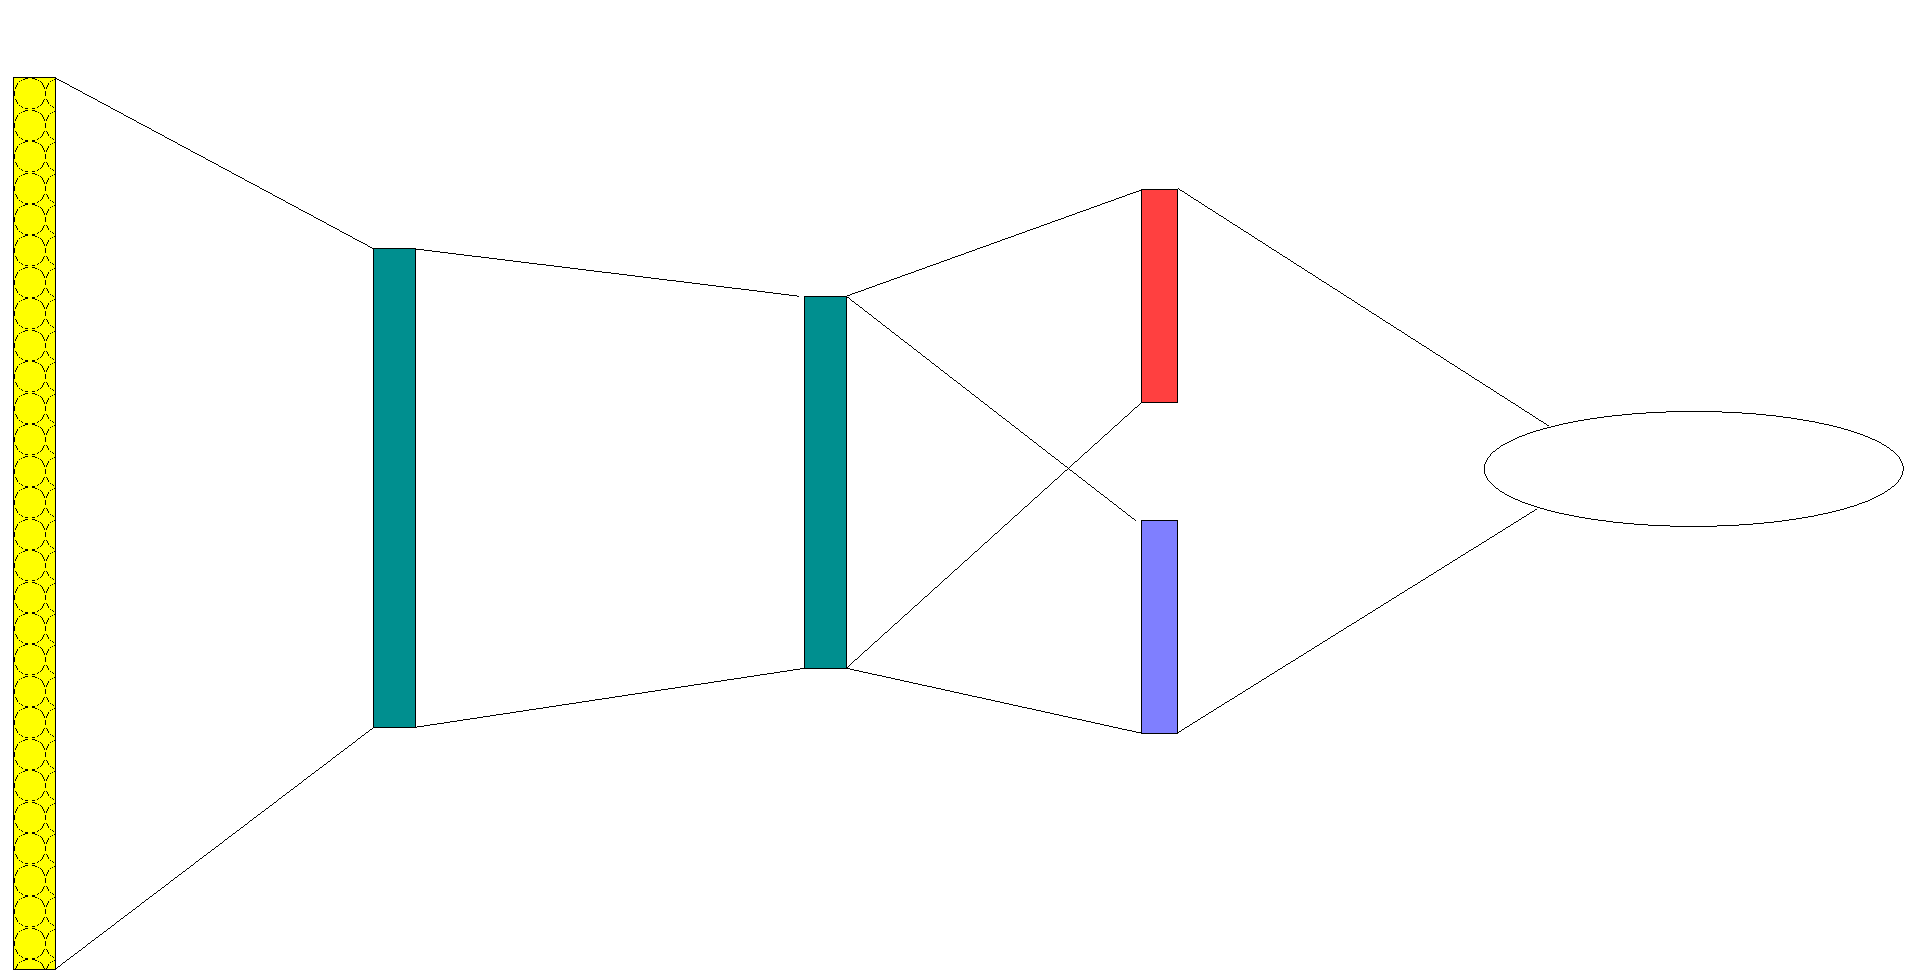
\includegraphics{figures/archi.pdf}%
\end{picture}%
\setlength{\unitlength}{4144sp}%
%
\begingroup\makeatletter\ifx\SetFigFont\undefined%
\gdef\SetFigFont#1#2#3#4#5{%
  \reset@font\fontsize{#1}{#2pt}%
  \fontfamily{#3}\fontseries{#4}\fontshape{#5}%
  \selectfont}%
\fi\endgroup%
\begin{picture}(14512,7383)(3361,-7948)
\put(6121,-2131){\makebox(0,0)[lb]{\smash{{\SetFigFont{29}{34.8}{\rmdefault}{\mddefault}{\updefault}$n_1^h$}}}}
\put(3376,-916){\makebox(0,0)[lb]{\smash{{\SetFigFont{29}{34.8}{\rmdefault}{\mddefault}{\updefault}$n^v$}}}}
\put(7066,-6676){\makebox(0,0)[lb]{\smash{{\SetFigFont{20}{24.0}{\rmdefault}{\mddefault}{\updefault}hidden layers}}}}
\put(10441,-5236){\makebox(0,0)[lb]{\smash{{\SetFigFont{20}{24.0}{\rmdefault}{\mddefault}{\updefault}soft max}}}}
\put(10036,-3076){\makebox(0,0)[lb]{\smash{{\SetFigFont{20}{24.0}{\rmdefault}{\mddefault}{\updefault}fully connected}}}}
\put(7021,-4246){\makebox(0,0)[lb]{\smash{{\SetFigFont{20}{24.0}{\rmdefault}{\mddefault}{\updefault}fully connected}}}}
\put(11926,-1321){\makebox(0,0)[lb]{\smash{{\SetFigFont{29}{34.8}{\rmdefault}{\mddefault}{\updefault}$2n$}}}}
\put(9406,-2131){\makebox(0,0)[lb]{\smash{{\SetFigFont{29}{34.8}{\rmdefault}{\mddefault}{\updefault}$n_2^h$}}}}
\put(3421,-4471){\makebox(0,0)[lb]{\smash{{\SetFigFont{50}{60.0}{\rmdefault}{\mddefault}{\updefault}$X$}}}}
\put(15166,-4246){\makebox(0,0)[lb]{\smash{{\SetFigFont{29}{34.8}{\rmdefault}{\mddefault}{\updefault}$(\hat y(x),\hat I(x))$}}}}
\put(12061,-2941){\makebox(0,0)[lb]{\smash{{\SetFigFont{50}{60.0}{\rmdefault}{\mddefault}{\updefault}$\hat {\bf y}$}}}}
\put(12061,-5506){\makebox(0,0)[lb]{\smash{{\SetFigFont{50}{60.0}{\rmdefault}{\mddefault}{\updefault}$\hat {\bf p}$}}}}
\end{picture}%
}}
\caption{\label{fig:archi} Architecture of the neural network specified by the number of units 
$(n^v,n_1^h,n_2^h,2\vert T\vert)$ in each layer.}
\label{fig:NN}
\end{figure}

\section{Experimental Setting}\label{sec:pdtExp}

\begin{table}[ht]
  \caption{
    Synthetic and Real-World Problems. 
    For the solar wind problem, training and test data sizes represent one cross validation fold}
  \label{tab:exp_data_info}
  \centering
  \begin{tabular}{ r c c c c}
  \hline
  Problem &  \# train & \# test & $d$ & $|T|$ \\
  \hline
  \textbf{I} & $10,000$ & $2,000$  & $10$ & $15$\\
  \textbf{II} & $10,000$ & $2,000$ & $10$ & $20$\\
  \textbf{III} & $10,000$ & $2,000$ & $10$ & $20$\\
  \textbf{IV} & $10,000$ & $2,000$ & $10$ & $20$\\
  \textbf{Solar Wind} & $77,367$ & $648$ & $374$ & $12$\\
  \hline
  \end{tabular}
\end{table}

%Proofs of concept for the  \XX\ algorithm are obtained using synthetic problems as well as our real-world %motivating application, the prediction of the solar wind (\cref{sec:intro}). 
The goal of the experiments is twofold. Firstly, the \XX\ predictive performance is assessed by 
considering 
%
\begin{enumerate*} 
  \item the RMSE of the predicted effect series $\hat y_m$, computed from Eq. (\ref{prop:opred})  
  \item the accuracy of the time lag prediction 
\end{enumerate*}. 
%
The latter performance indicator is measured and compared to the ground truth using synthetic 
problems, detailed below: although time lag relationships do exist in real world data sets 
\citep{doi:10.1002/jgra.50429,ZHOU2006195}, we are not aware of datasets with time lag 
relationships explicitly annotated. The former performance indicator is comparatively assessed 
using the naive baseline, the regression model computed by assuming a fixed time lag set to 
$\frac{\tau_{min}+\tau_{max}}{2}$. The Pearson correlation of the true $y_m$ and predicted 
$\hat y_m$ series is also considered as overall performance indicator of the prediction.

The second goal of experiments is to determine how informative are the key statistical quantities 
$\sigma_0$ and $C_1$ (\cref{sec:stability}), and whether they can effectively be used as 
measures of confidence about the prediction results. Table \ref{tab:exp_data_info} summarises the 
dimensions of the synthetic and real problems used as proofs of concept for the \XX\ validation. 

\paragraph{Synthetic Problems} 
The driving force $x_m$, of the artificial system is generated in $\mathbb{R}^{10}$ using 
\emph{Stochastic Langevin Dynamics} (with $\eta = 0.02, s^2 = 0.7$); the time series $y_m$ is 
generated using the norm of $x_m$:
% 
\begin{align}
 x_{m+1} &= (1 - \eta) x_m + \mathcal{N}(0, s^2) \label{eq:data}\\
 y_{m+\tau(x_m)} &= k ||x_m||^2 + c \label{eq:outputs}
\end{align}
%
Four models of increasing complexity have been used for the time lag relationship $\tau(x_m)$; the 
width of the time lag interval $|T|$ is set to $20$ except for Problem I where it is set to $15$.
\\\\
%
{\bf Problem I}: Constant time lag $\tau(x_m) = 5$\\
%
In all other problems, the time lag $\tau(x_m)$ depends on the velocity $v_m = k ||x_m||^2 + c$\\
%
{\bf Problem II}: Constant velocity $\tau(x_m) = 100/v_m,\ k = 1,\ c = 10$\\
%
{\bf Problem III}: Constant acceleration 
$\tau(x_m) = (\sqrt{v_m^2 + 2ad} - v)/a,\ k = 5,\ a = 5,\ d = 1000, \ c = 100$
\\
%
{\bf Problem IV}: Softplus 
$\tau(x_m) = \exp\left(v_m\right)/\left(1 + \exp(v_m/20)\right), \ k = 10, c = 40$\\

\paragraph{Solar Wind Speed Prediction}\label{sec:solarwind}
As said in \cref{sec:motivationsolarwind}, the task of predicting solar wind speed from 
heliospheric data not only has scientific significance; it is also challenging due to the distance 
between the Sun and the Earth and the non-stationary propagation time of the solar plasma through 
the interplanetary medium. 

The inputs $x_m$ are compiled from two sources, synoptic Carrington maps of the photospheric 
magnetic field taken from the \emph{Global Oscillation Network Group} (GONG) and solar activity 
proxies taken from the OMNI data set \footnote{\url{https://omniweb.gsfc.nasa.gov}}. Specifically, 
$x_m$ is a vector consisting of the components outlined in \cref{table:dtlrInputs}.

For each input pattern, time lagged solar wind data is extracted corresponding to minimum and 
maximum time delays of two and five days respectively. For computational convenience, each three 
day time window is pre-processed by computing sliding six hour medians yielding $|T| = 12$ time 
slots.
%
\begin{table}[ht]
    \centering
    \begin{tabular}{l l l p{0.4\textwidth}}
        \hline
        \textbf{Quantity} & \textbf{Source} & \textbf{Domain} & \textbf{Notes}\\
        \hline
        \vspace{5pt}
          $\log \mathbf{f}_S$ & 
          GONG & 
          $\mathbb{R}^{180}$ & 
          $\mathbf{f}_S$ or FTE is computed from the outputs of the CSSS model.\\
          $\mathbf{B}_{ss}$ & 
          GONG & 
          $\mathbb{R}^{180}$  & 
          The radial magnetic field strength on the solar source surface is the primary output computed by the CSSS model.\\
          $\Phi$ & 
          GONG & 
          $[0, 360)$ & 
          $\Phi$ is the Carrington longitude of the computed $\mathbf{f}_S$.\\
          $\mathbf{v}_{27}$ & 
          OMNI & 
          $\mathbb{R}^{\rvert T \rvert}$ & 
          $\mathbf{v}_{27}$ is the solar wind speed recorded $27$ days prior, one for each value of the forward time window. \\
          $\mathrm{SSN}$ & OMNI & $\mathbb{R}^{+}$ & The sun spot number measures the number of visible sun spots on the solar disk. \\
          $\mathrm{F}10.7$ & OMNI & $\mathbb{R}^{+}$ & $\mathrm{F}10.7$ is the measured solar radio flux. \\
        \hline
    \end{tabular}
    \caption{Inputs used in the DTLR solar wind forecast model.}
    \label{table:dtlrInputs}
\end{table}
%
\XX\ is validated using a $9$ fold cross-validation, where the test data consists of one 
(continuous) Carrington rotation (see \cref{table:dtlrsplits}). The performance on Carrington 
rotation $2077$ (first fold in \cref{table:dtlrsplits}) is compared with the state of the art 
\citep{Riley2011} in \cref{tab:results_riley}, while the overall cross-validation performance 
is compared with a fixed time lag baseline which uses the same inputs as the DTLR model 
(\cref{table:dtlrInputs}) and has the same architecture until the penultimate layer 
(\cref{fig:archi}). 
%
\begin{table}[ht]
  \centering
  \caption{Cross validation splits used to evaluate \ \XX \ on the solar wind forecasting task}
  \label{table:dtlrsplits}
  \begin{tabular}{llll}
  \hline
  \textbf{Split Id} & \textbf{Carrington Rotation} & \textbf{Start} & \textbf{End}\\ \hline
  $1$ & $2077$ & 2008/11/20 07:00:04 & 2008/12/17 14:38:34  \\
  $2$ & $2090$ & 2009/11/09 20:33:43 & 2009/12/07 04:03:59  \\
  $3$ & $2104$ & 2010/11/26 17:32:44 & 2010/12/24 01:15:56  \\
  $4$ & $2117$ & 2011/11/16 07:04:41 & 2011/12/13 14:39:28  \\
  $5$ & $2130$ & 2012/11/04 20:39:43 & 2012/12/02 04:06:23  \\
  $6$ & $2143$ & 2013/10/25 10:17:52 & 2013/11/21 17:36:35  \\
  $7$ & $2157$ & 2014/11/11 07:09:56 & 2014/12/08 14:41:02  \\
  $8$ & $2171$ & 2015/11/28 04:09:27 & 2015/12/25 11:53:33  \\
  $9$ & $2184$ & 2016/11/16 17:41:04 & 2016/12/14 01:16:43  \\
  \hline
  \end{tabular}
  \end{table}
%


\section{Empirical validation}\label{sec:proofconcept}

\begin{figure*}
  \centering

  \begin{subfigure}[b]{0.4\textwidth}
    \centering
    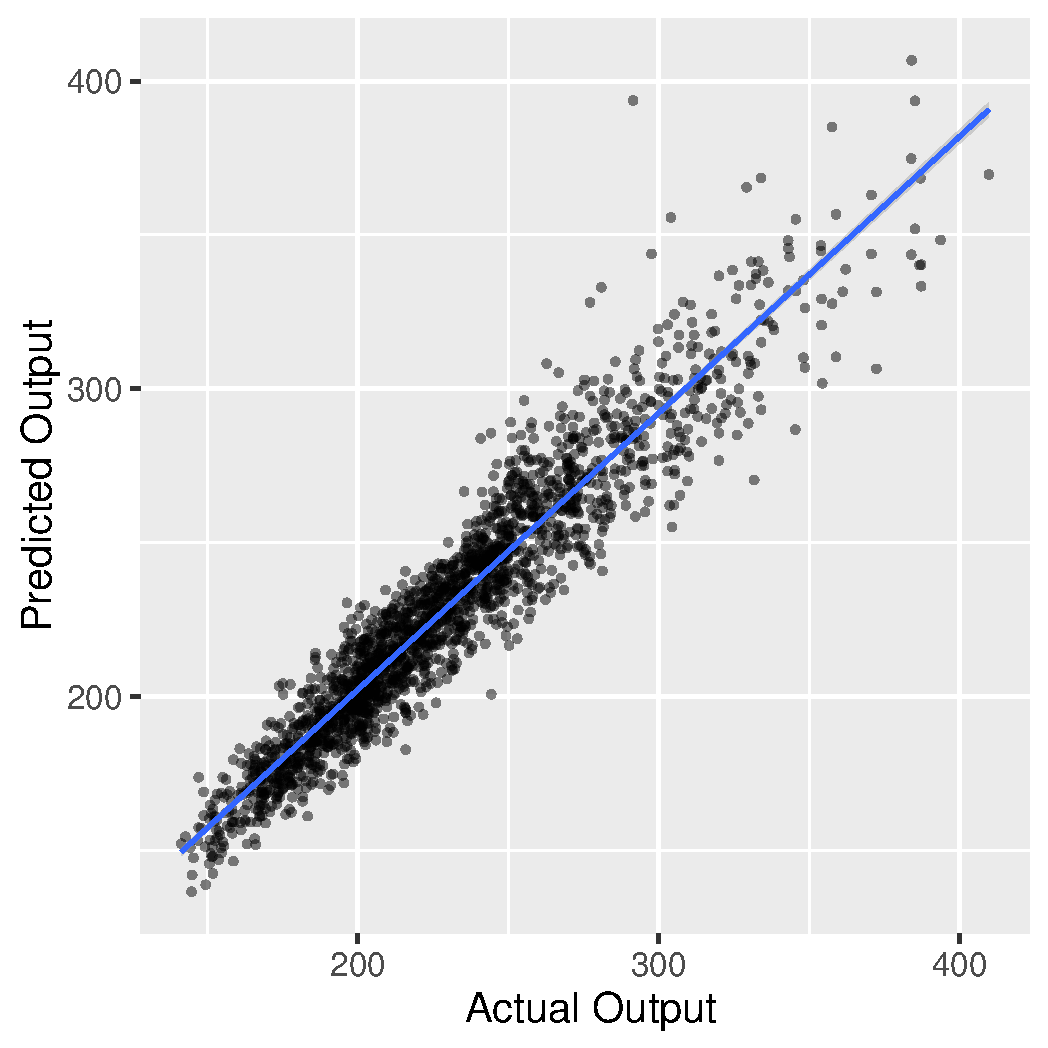
\includegraphics[width=\textwidth]{figures/exp2_scatter_v_test}
    \caption{ \textbf{Problem II}, Goodness of fit, Output $y(x)$}
    \label{fig:problem2_fitv}
  \end{subfigure}
  \hfill
  \begin{subfigure}[b]{0.4\textwidth}
    \centering
    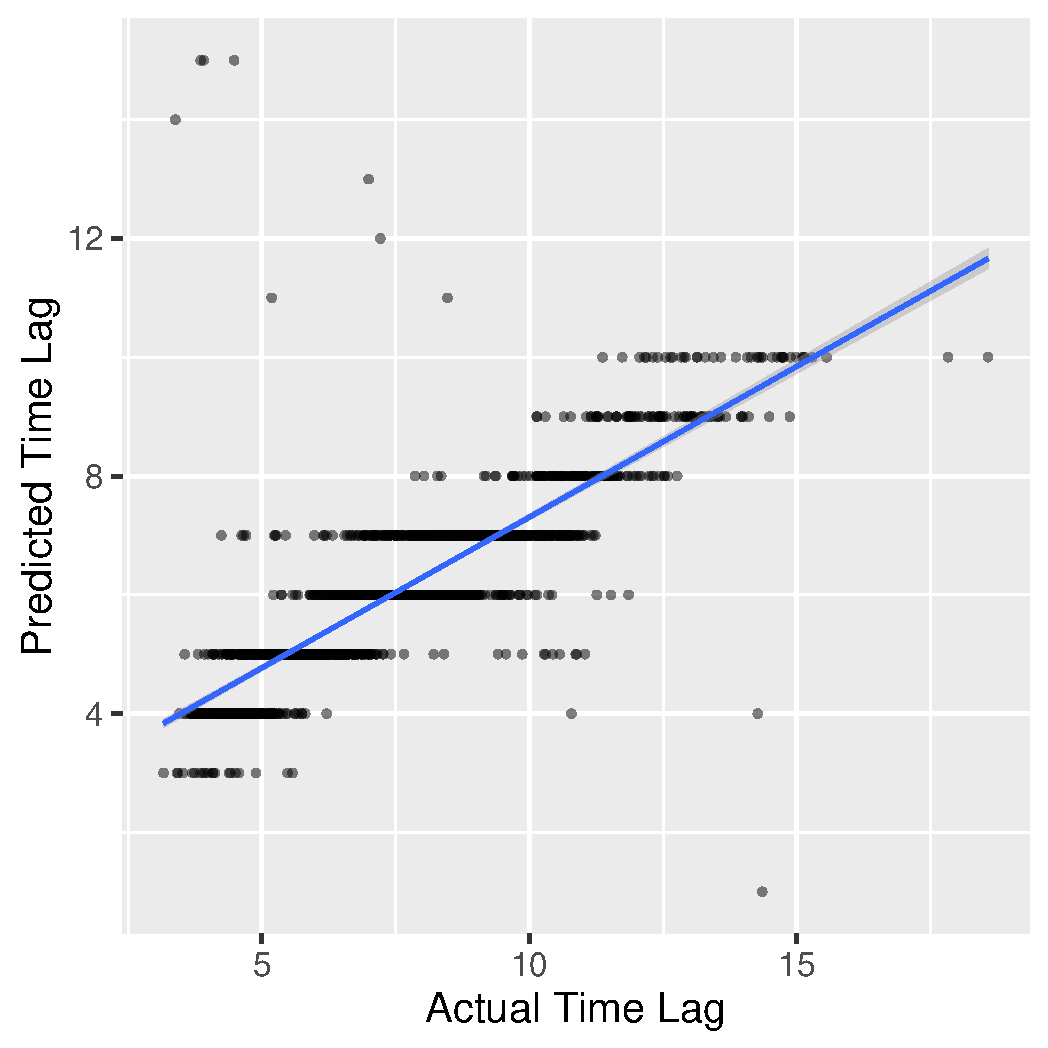
\includegraphics[width=\textwidth]{figures/exp2_scatter_t_test}
    \caption{ \textbf{Problem II}, Goodness of fit, Time lag $\tau(t)$ }
    \label{fig:problem2_fitt}
  \end{subfigure}
  
  \vskip\baselineskip
  
  \begin{subfigure}[b]{0.4\textwidth}
    \centering
    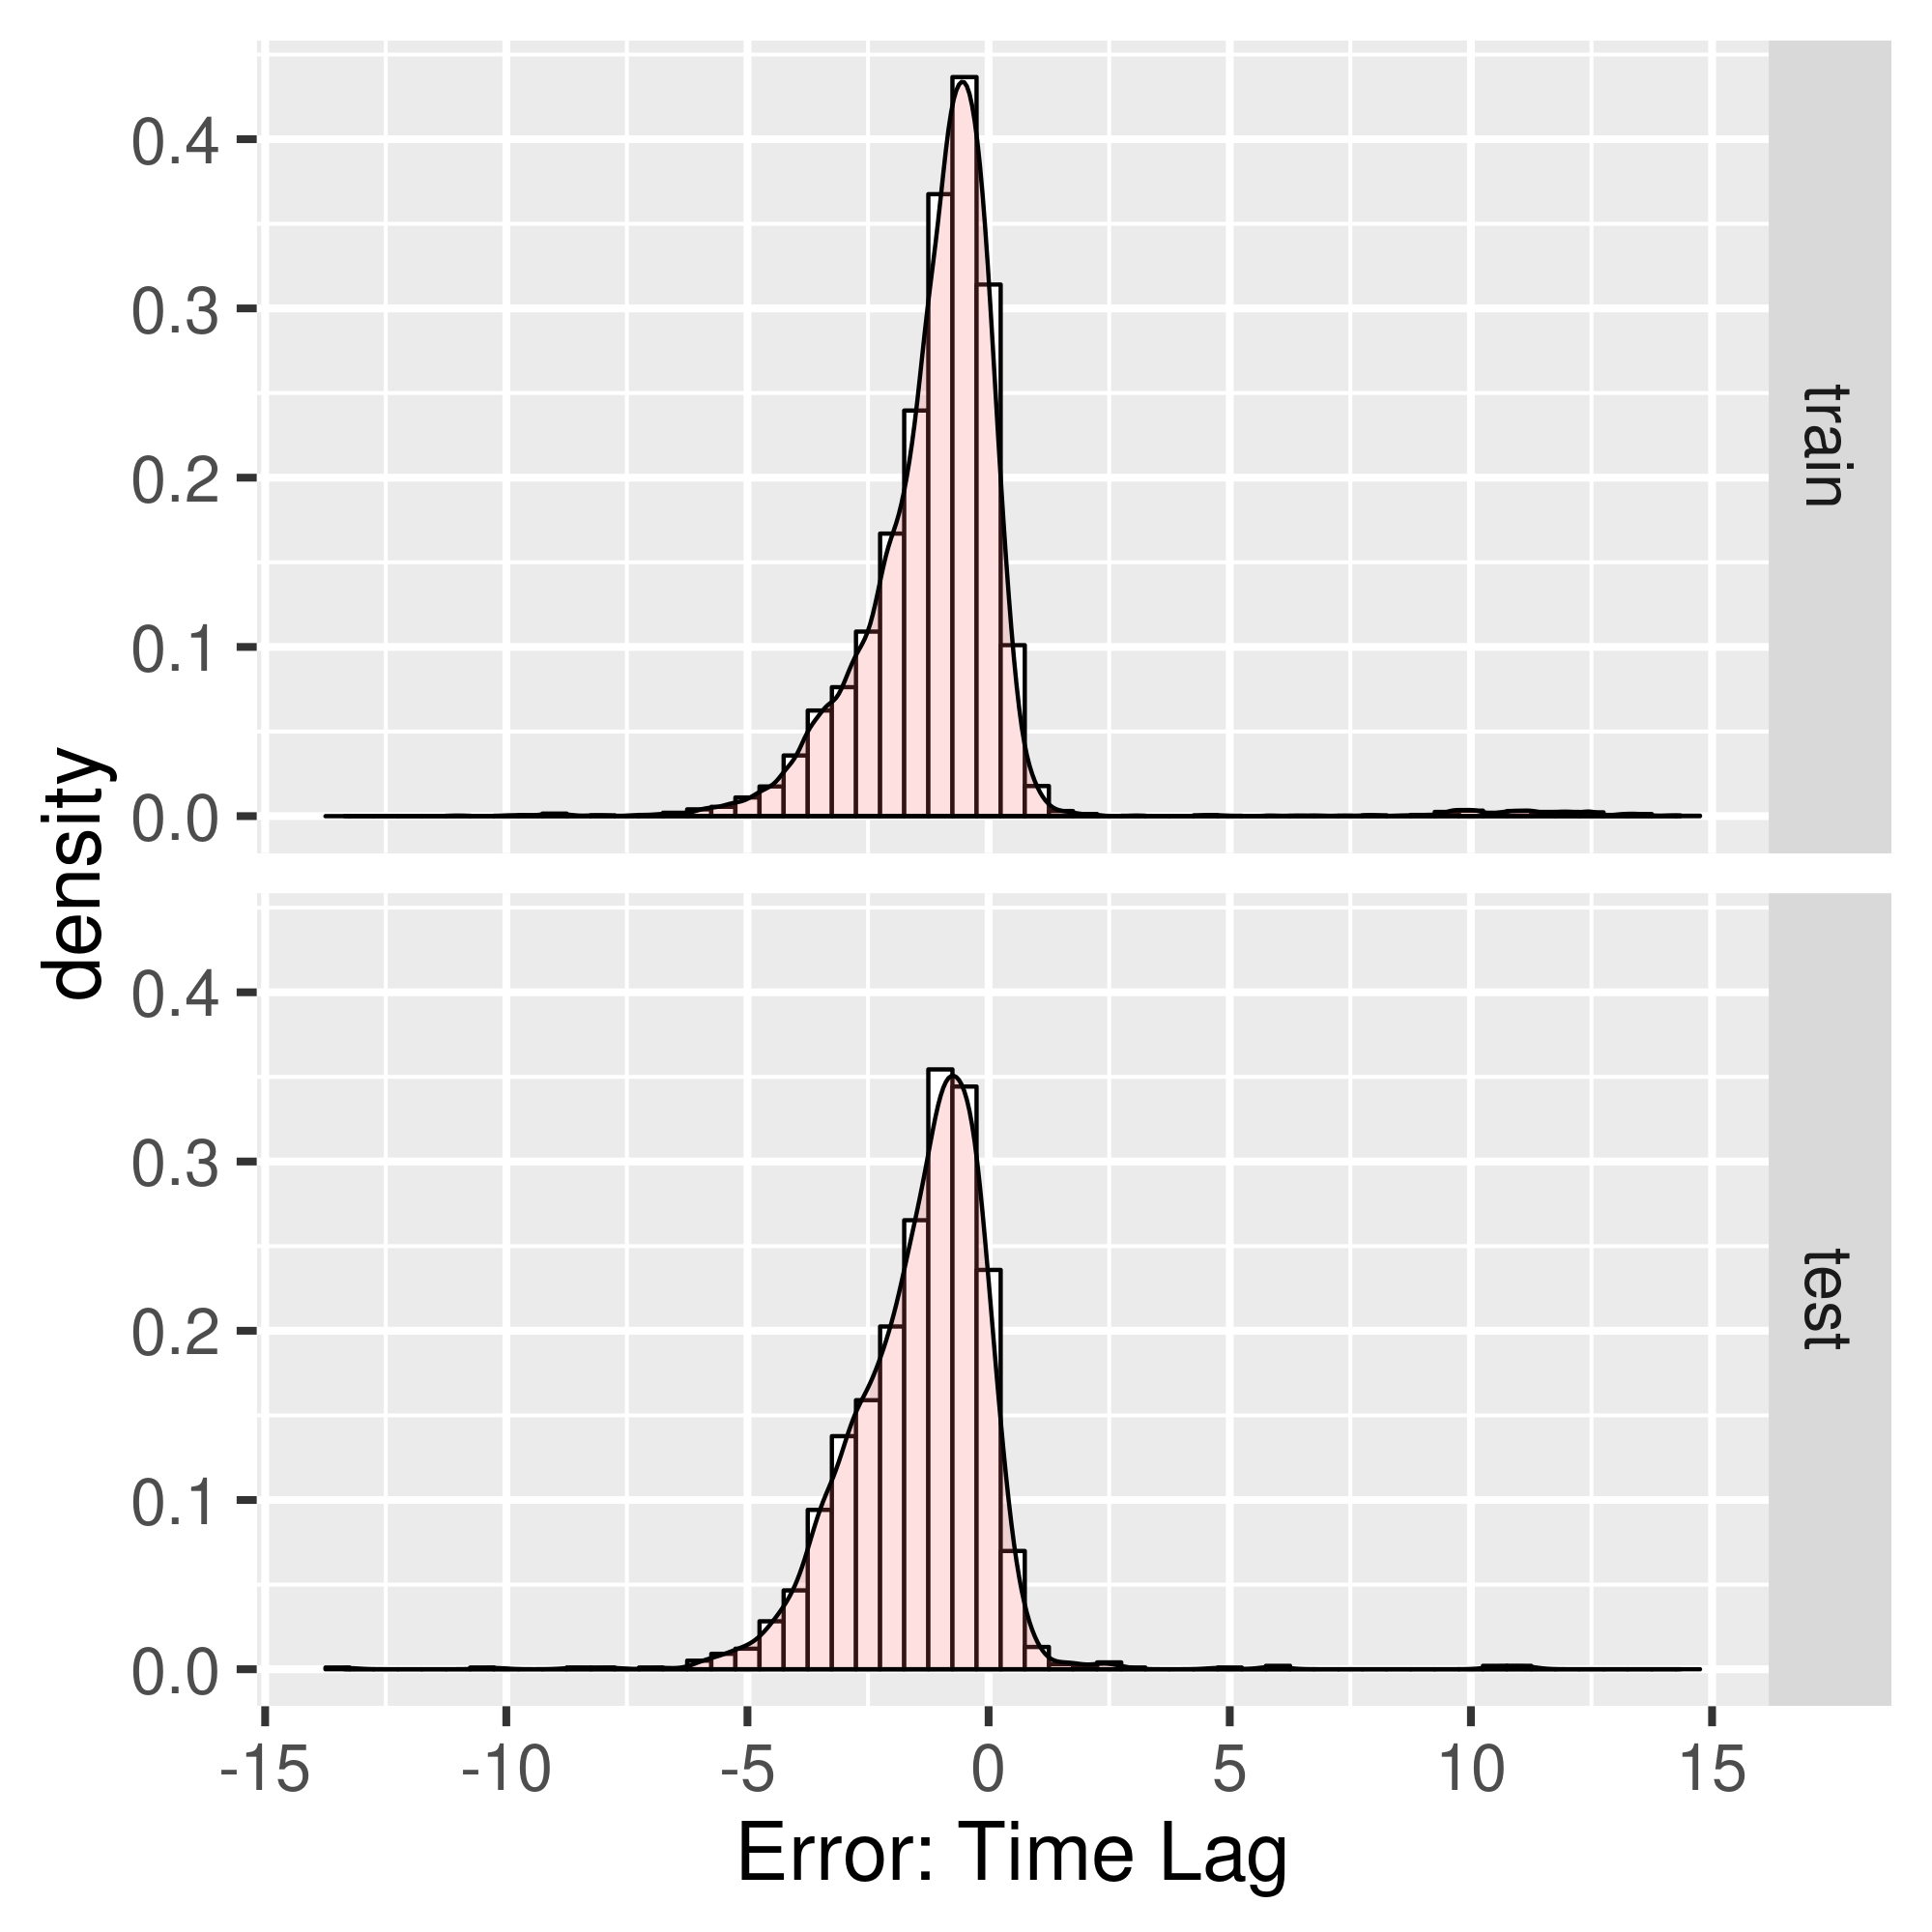
\includegraphics[width=\textwidth]{figures/exp2_hist_errors_timelag}
    \caption{ \textbf{Problem II}, Error of time lag prediction} 
    \label{fig:problem2_error}
  \end{subfigure}
  \hfill
  \begin{subfigure}[b]{0.4\textwidth}
    \centering
    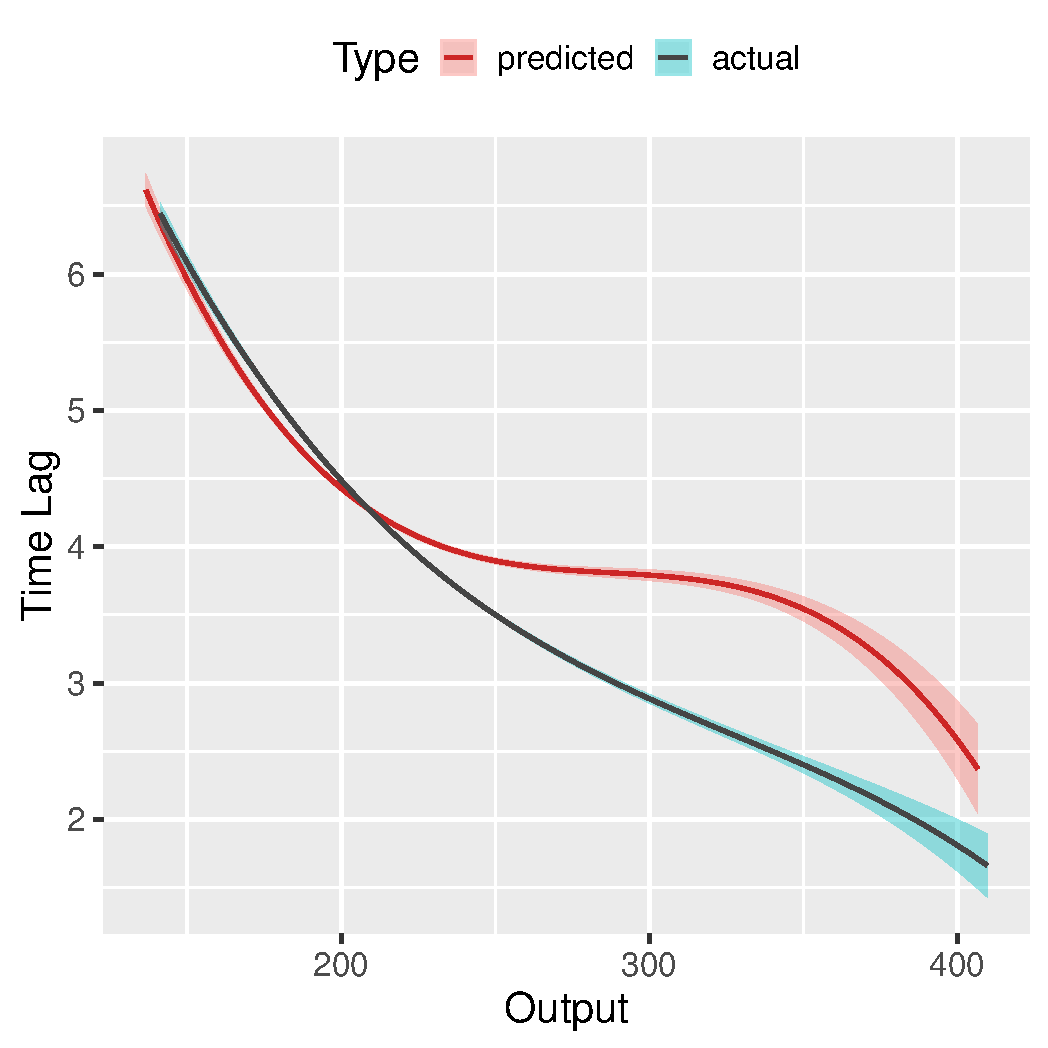
\includegraphics[width=\textwidth]{figures/exp2_predictive_curves}
    \caption{ \textbf{Problem II}, Output vs Time Lag Relationship} 
    \label{fig:problem2_curves}
  \end{subfigure}

  %\vskip\baselineskip
  
  %\begin{subfigure}[b]{0.4\textwidth}
  %  \centering
  %  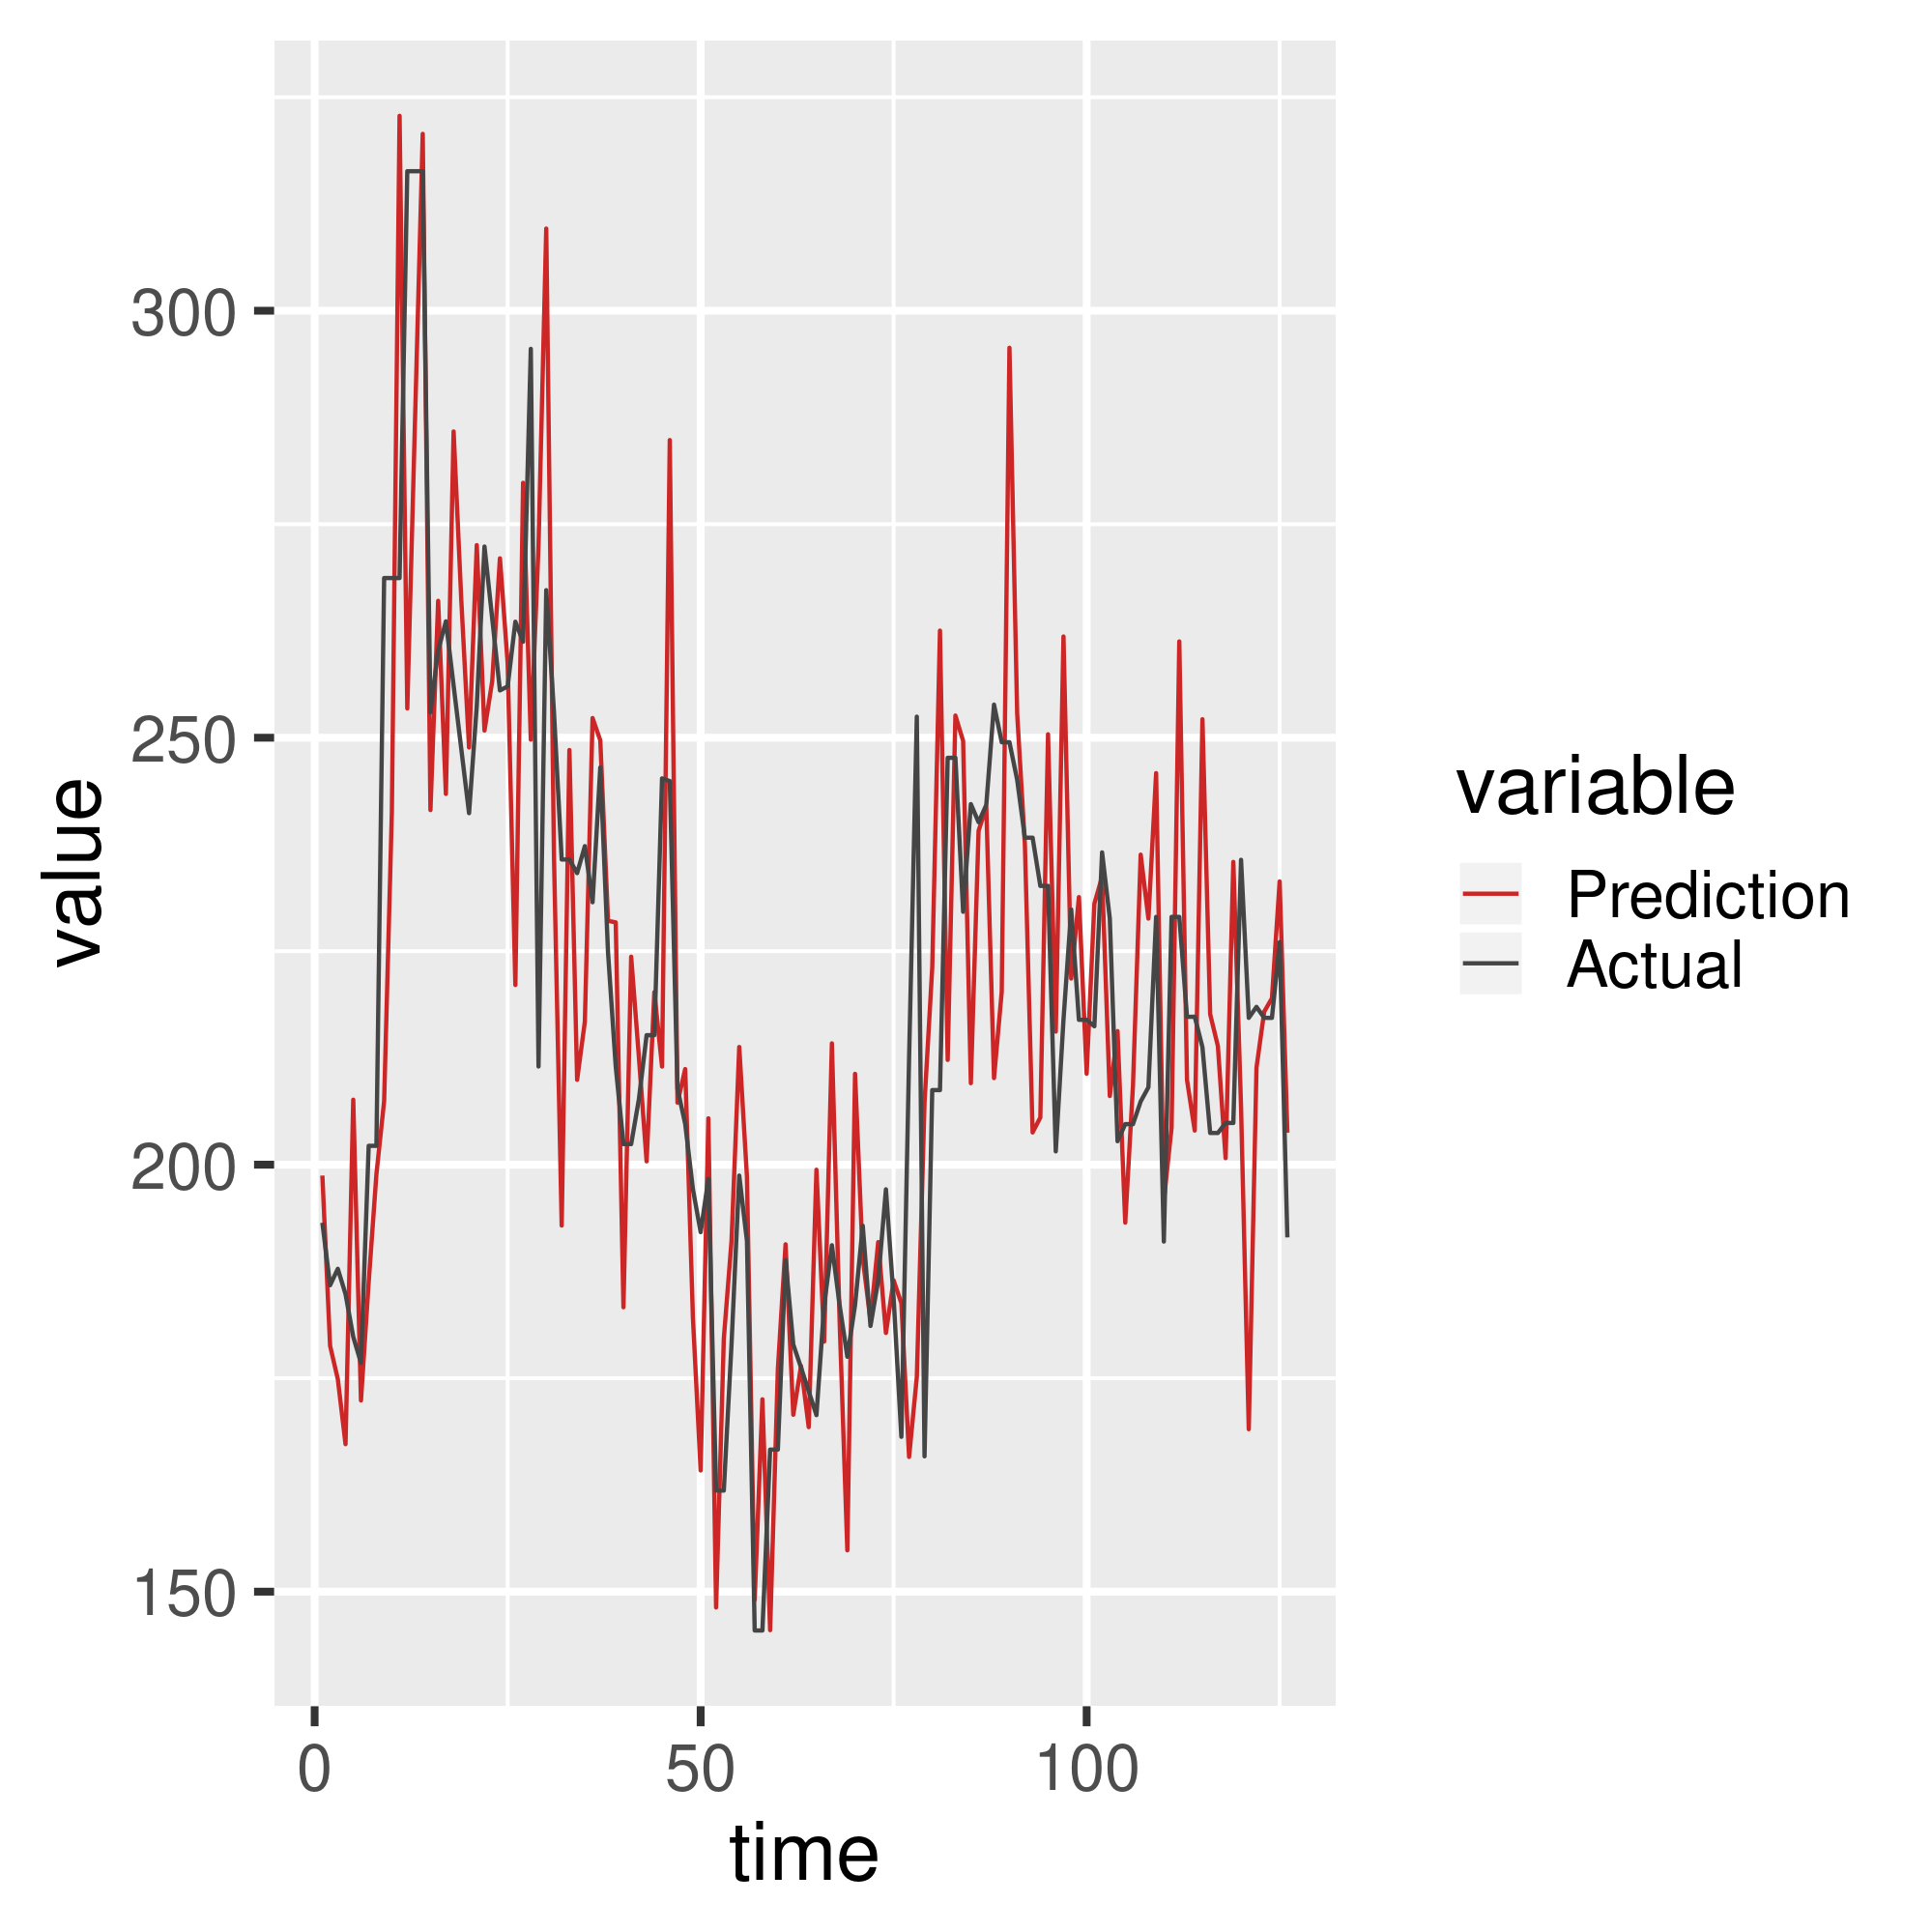
\includegraphics[width=\textwidth]{figures/exp2_timeseries_pred}
  %  \caption{ \textbf{Problem II}, A portion of the test time series reconstructed using the model} 
  %  \label{fig:problem2_timeseries}
  %\end{subfigure}
  %\hfill
  %\begin{subfigure}[b]{0.4\textwidth}
  %  \centering
  %  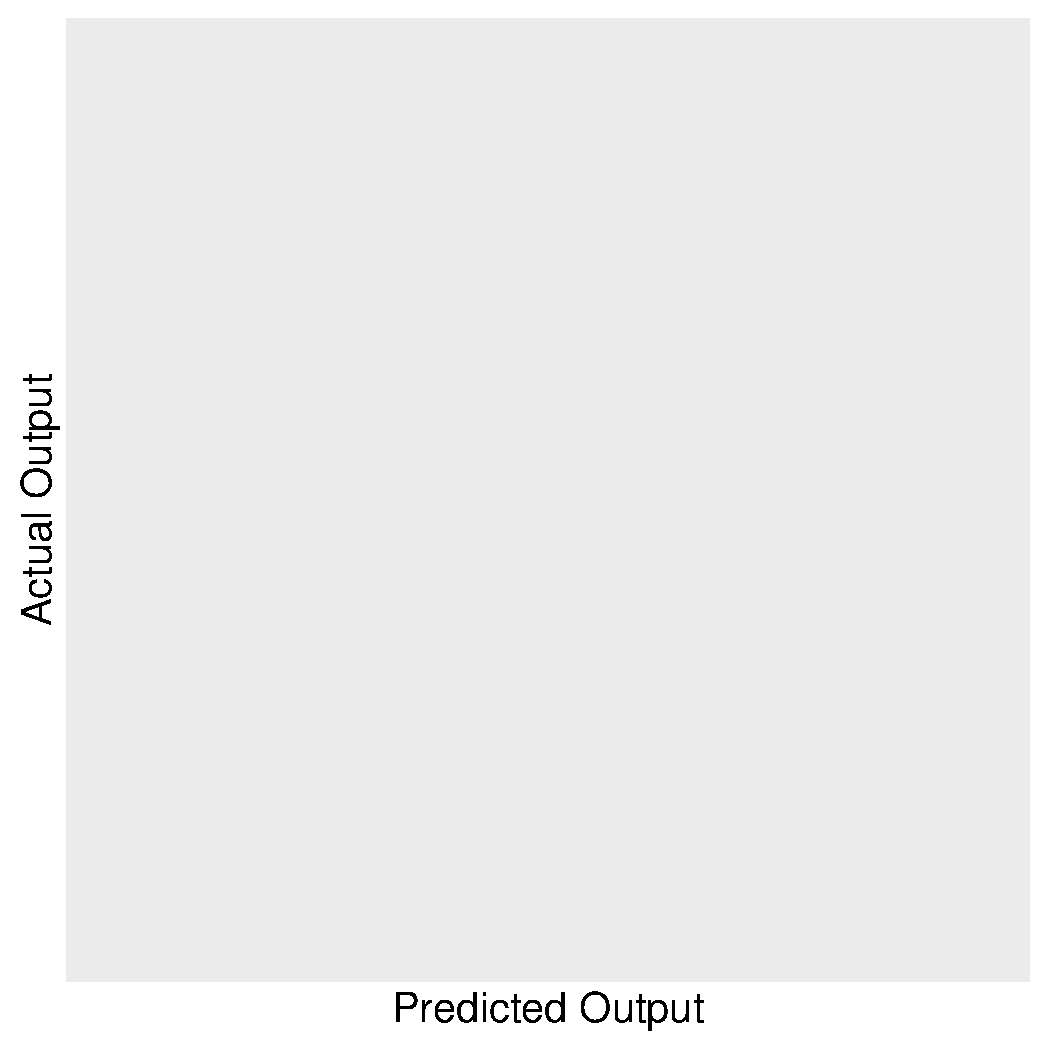
\includegraphics[width=\textwidth]{figures/exp2_lag_error_jus}
  %  \caption{ \textbf{Problem II}, Predicted vs Actual Outputs for the cases with time lag error $\leq -2.5$.} 
  %  \label{fig:problem2_lag_error_jus}
  %\end{subfigure}
  
  \caption{\textbf{Problem II}, Results}
\end{figure*}

\begin{figure*}
  \centering

  \begin{subfigure}[b]{0.4\textwidth}
    \centering
    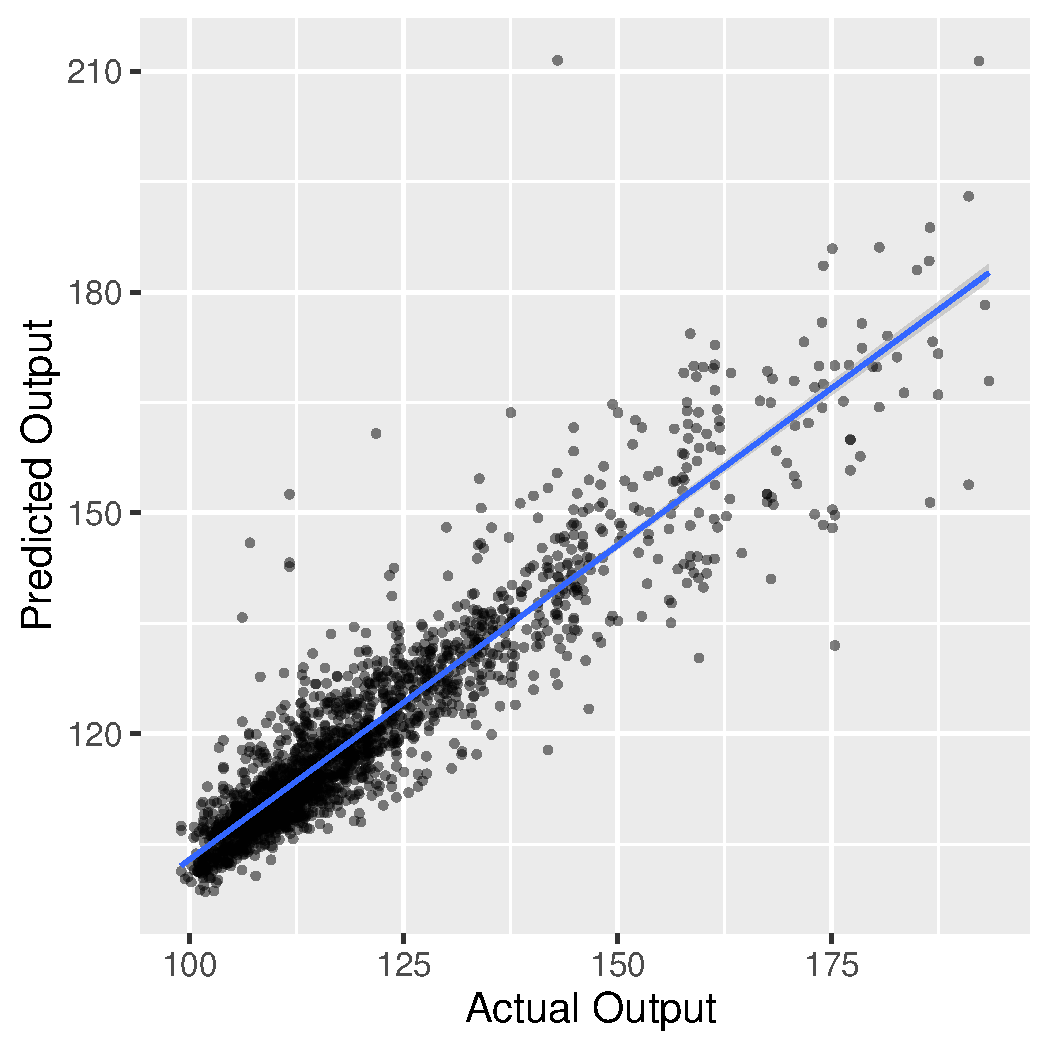
\includegraphics[width=\textwidth]{figures/exp3_scatter_v_test}
    \caption{ \textbf{Problem III}, Goodness of fit, Output $y(x)$}
    \label{fig:problem3_fitv}
  \end{subfigure}
  \hfill
  \begin{subfigure}[b]{0.4\textwidth}
    \centering
    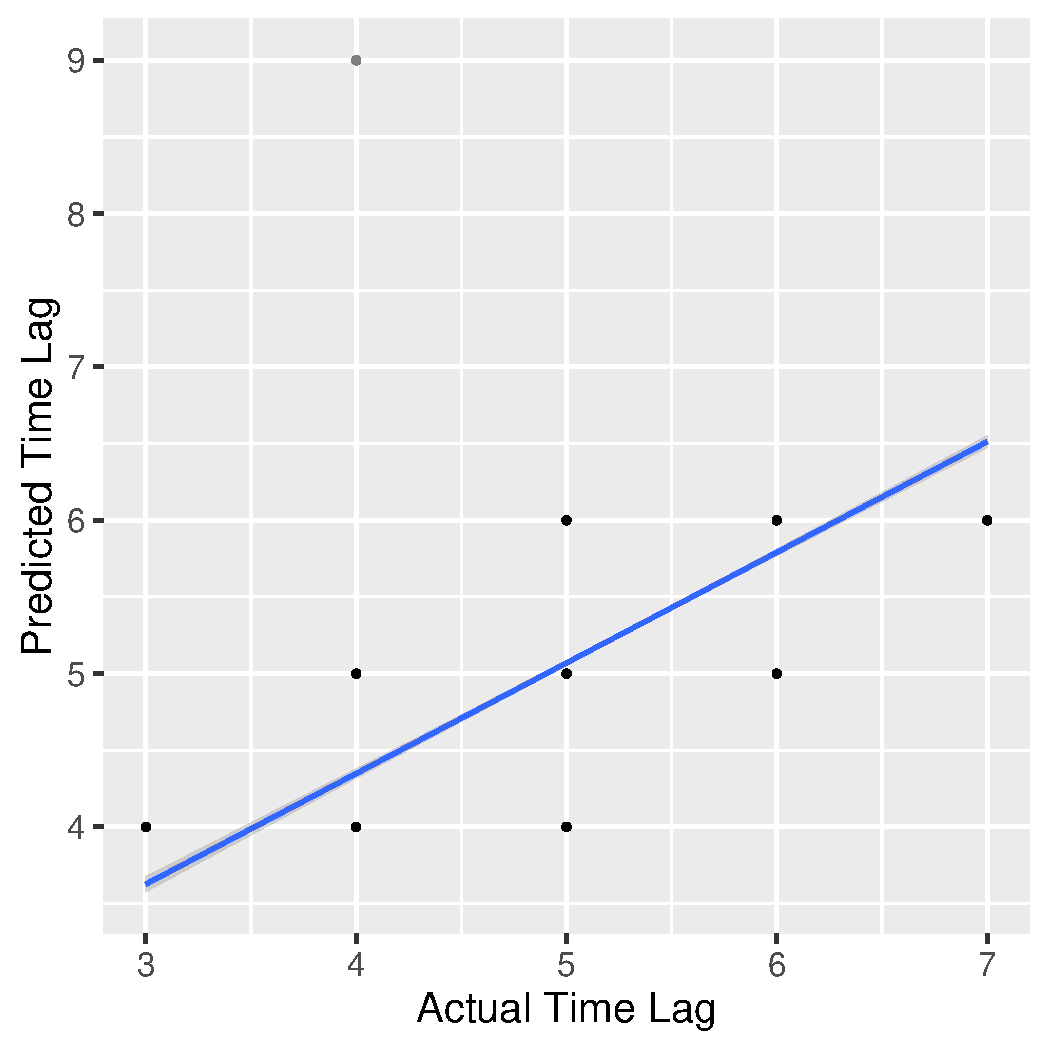
\includegraphics[width=\textwidth]{figures/exp3_scatter_t_test}
    \caption{ \textbf{Problem III}, Goodness of fit, Time lag $\tau(t)$ }
    \label{fig:problem3_fitt}
  \end{subfigure}

  \vskip\baselineskip
  
  \begin{subfigure}[b]{0.4\textwidth}
    \centering
    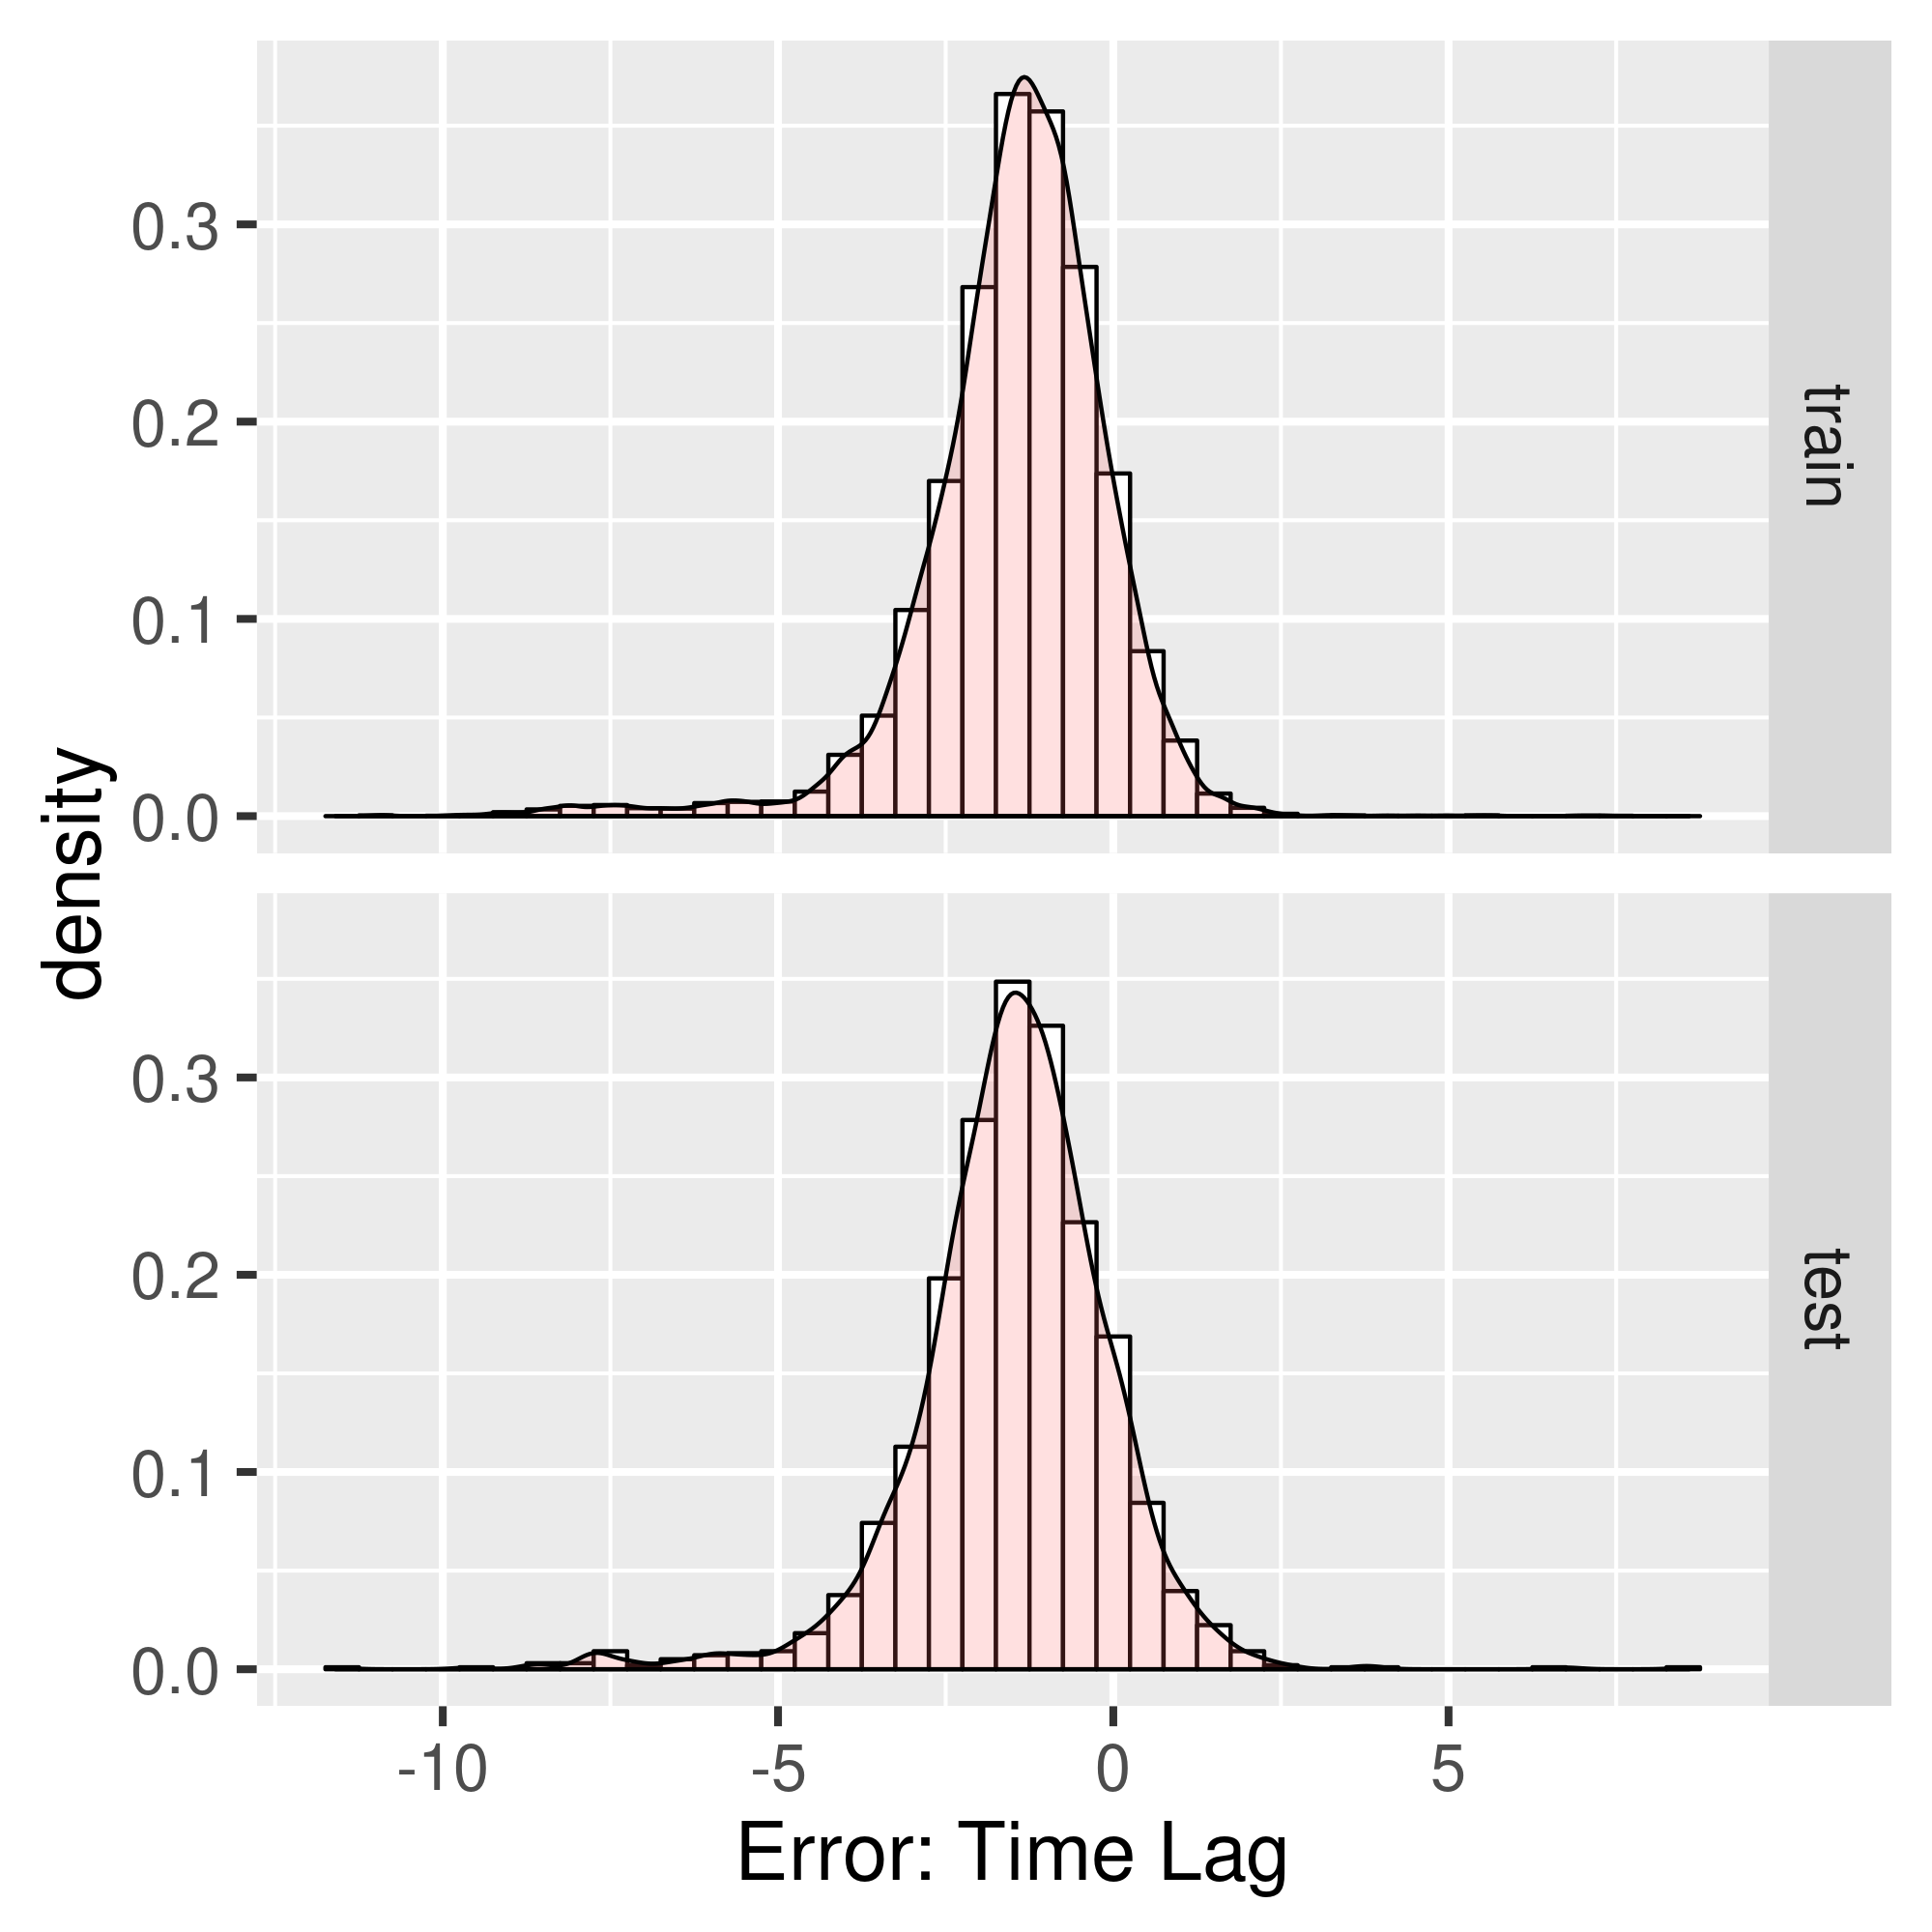
\includegraphics[width=\textwidth]{figures/exp3_hist_errors_timelag}
    \caption{ \textbf{Problem III}, Error of time lag prediction} 
    \label{fig:problem3_error}
  \end{subfigure}
  \hfill
  \begin{subfigure}[b]{0.4\textwidth}
    \centering
    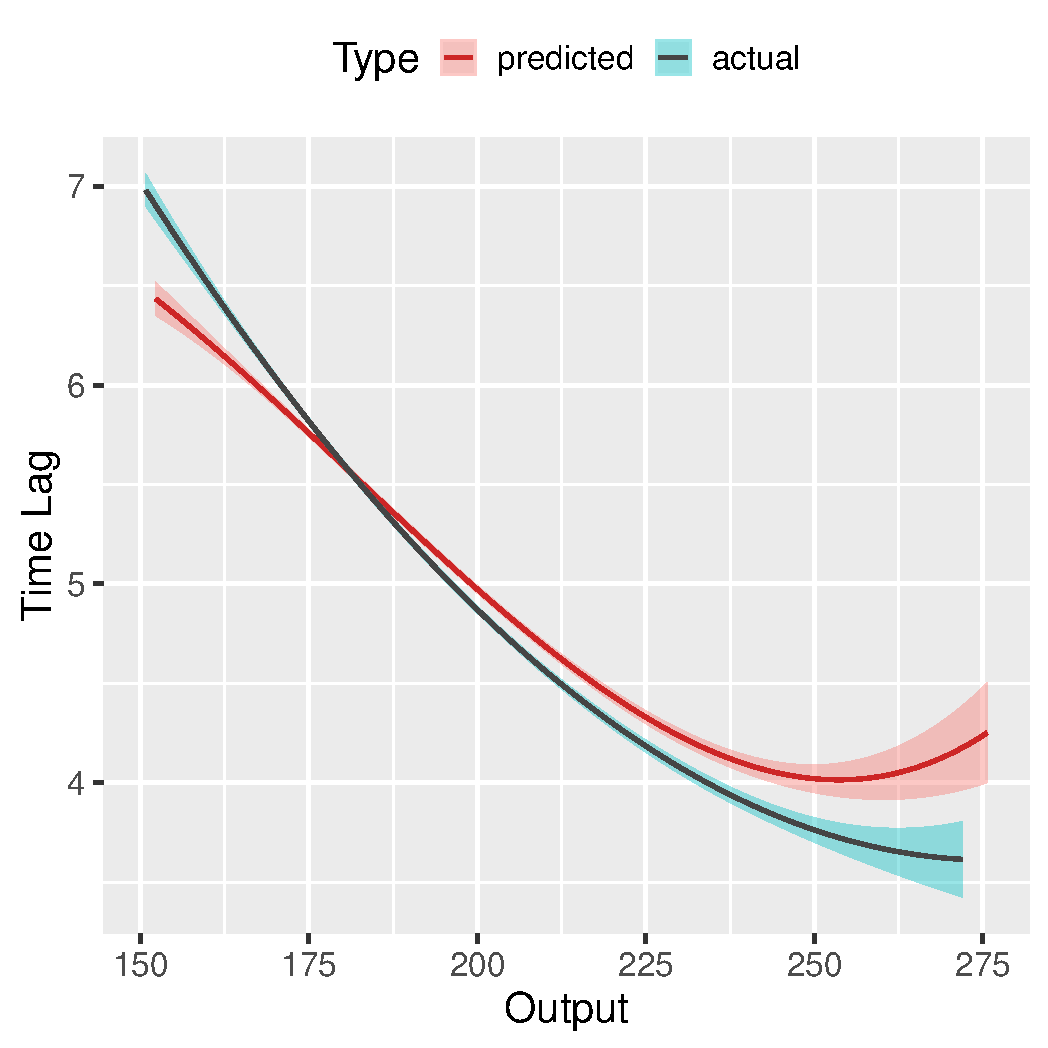
\includegraphics[width=\textwidth]{figures/exp3_predictive_curves}
    \caption{ \textbf{Problem III}, Output vs Time Lag Relationship} 
    \label{fig:problem3_curves}
  \end{subfigure}
  
  %\vskip\baselineskip
  
  %\begin{subfigure}[b]{0.4\textwidth}
  %  \centering
  %  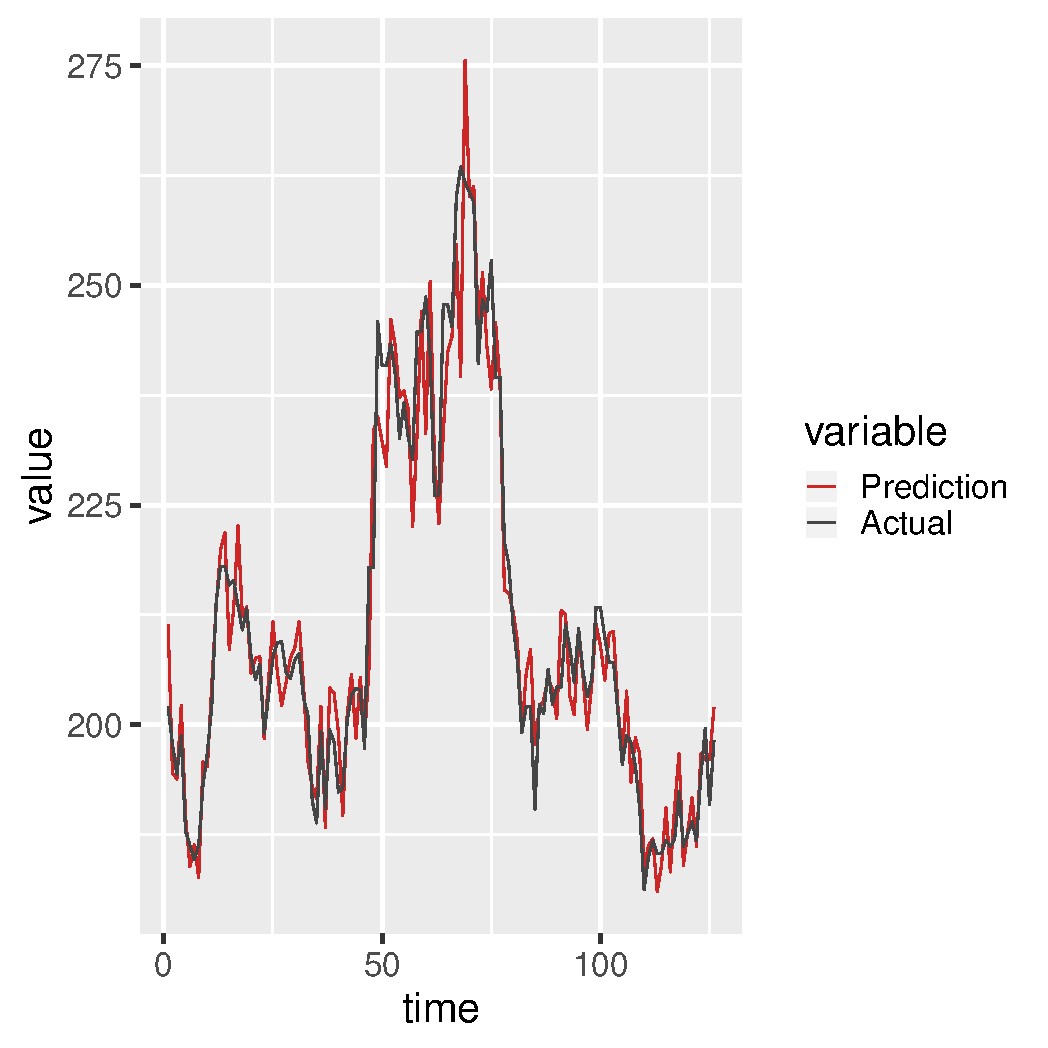
\includegraphics[width=\textwidth]{figures/exp3_timeseries_pred}
  %  \caption{ \textbf{Problem III}, A portion of the test time series reconstructed using the model} 
  %  \label{fig:problem3_timeseries}
  %\end{subfigure}
  %\hfill
  %\begin{subfigure}[b]{0.4\textwidth}
  %  \centering
  %  \includegraphics[width=\textwidth]{figures/exp3_lag_error_jus}
  %  \caption{ \textbf{Problem III}, Predicted vs Actual Outputs for the cases with time lag error $\leq -2.5$.} 
  %  \label{fig:problem3_lag_error_jus}
  %\end{subfigure}
  
  \caption{\textbf{Problem III}, Results}
\end{figure*}

\begin{figure*}
  \centering

  \begin{subfigure}[b]{0.4\textwidth}
    \centering
    \includegraphics[width=\textwidth]{figures/exp4_scatter_v_test}
    \caption{ \textbf{Problem IV}, Goodness of fit, Output $y(x)$}
    \label{fig:problem4_fitv}
  \end{subfigure}
  \hfill
  \begin{subfigure}[b]{0.4\textwidth}
    \centering
    \includegraphics[width=\textwidth]{figures/exp4_scatter_t_test}
    \caption{ \textbf{Problem IV}, Goodness of fit, Time lag $\tau(t)$ }
    \label{fig:problem4_fitt}
  \end{subfigure}
  
  \vskip\baselineskip
  
  \begin{subfigure}[b]{0.4\textwidth}
    \centering
    \includegraphics[width=\textwidth]{figures/exp4_hist_errors_timelag}
    \caption{ \textbf{Problem IV}, Error of time lag prediction} 
    \label{fig:problem4_error}
  \end{subfigure}
  \hfill
  \begin{subfigure}[b]{0.4\textwidth}
    \centering
    \includegraphics[width=\textwidth]{figures/exp4_predictive_curves}
    \caption{ \textbf{Problem IV}, Output vs Time Lag Relationship} 
    \label{fig:problem4_curves}
  \end{subfigure}
  
  \caption{\textbf{Problem IV}, Results}
\end{figure*}


Table \ref{tab:results_syn} summarises the \XX\ performance on the synthetic and real-world 
problems, respectively compared to the naive baseline (constant time lag) and to the state of the 
art for the real-world solar wind problem. 

The values of the $\sigma_0$ and $C_1$ quantities involved in the stability analysis 
(\cref{sec:stability}) are also reported. As said, $C_1 < 1$ indicates a specialization 
among predictors found by the solution. The comparison of $\sigma_0$ and the RMSE indicates how 
better the learned model is compared to the trivial degenerate solution (uniform $\hat {\bf p}$, 
assigning an equal weight to all $\hat y_i$). Finally, the Pearson correlation between 
$\hat y_m$ and $y_m$ is reported; while its absolute value is less informative than it appears due 
to the auto-correlation of the series, it allows to compare different predictors. 

\begin{table}
  \caption{Performance: \XX  \ / Base Line / \XX  \ Time Lag Prediction}\label{tab:results_syn}
  \centering
  \begin{tabular}{ l l l l l l}
  \hline
  Problem &  M.A.E & R.M.S.E & Pearson Corr. & $\sigma_0$ & $C_1$\\
  \hline
  \textbf{Pb I} & $8.82$ / $21.79$ / $0.021$  & $12.35$ / $28.79$ / $0.26$ & $0.98$ / $0.87$ / -- & $29.8$ & $0.14$\\
  \textbf{Pb II} & $10.15$ / $27.40$ / $0.4$ & $13.70$ / $35.11$ / $0.67$ & $0.95$ / $0.73$ / $0.70$ & $26.83$ & $0.16$\\
  \textbf{Pb III} & $3.17$ / $11.01$ / $0.17$ & $4.63$ / $14.99$ / $0.42$ & $0.98$ / $0.79$ / $0.84$ & $11.84$ & $0.09$\\
  \textbf{Pb IV} & $3.88$ / $12.28$ / $0.34$ & $5.33$ / $15.89$ / $0.64$ & $0.98$ /$0.79$/ $0.81$ & $12.18$ & $0.13$\\
  \textbf{Solar Wind} & $56.35$ / $N.A$ / -- & $74.20$ / $N.A$ / -- & $0.6$ / $N.A$ / -- & $N.A$ & $N.A$\\
  \hline
  \end{tabular}
\end{table}
\todo{Update $\sigma_0$ and $C_1$ numbers for \XX in \cref{tab:results_syn}}

On the easy Problem I, the model predicts the correct time lag for $97.93\%$ of the samples. The 
higher value of $\sigma_0$ in problems I and II compared to the other problems is explained from 
the higher variance in the generated  time series $y(t)$. \\
On Problem II, the model accurately learns the inverse relationship between $x_m$, $\tau(x_m)$ and 
$y_m$ on average. The time lag is overestimated in the regions with low time lag 
(with high velocity), which is blamed on the low sample density in this region, due to the data 
generation process. \\
Interestingly, Problems III and IV are better handled by \XX, despite a more complex dynamic time 
lag relationship. In both latter cases however, the model tends to under-estimate the time lag in 
the high time lag regions and conversely to over-estimate it in the low time lag region. 

\begin{figure}
  \centering
  \includegraphics[width=0.4\textwidth]{figures/test_scatter_v}
  \caption{
    Predicted vs Actual Solar Wind Speed, 
    red diagonal represents a perfect prediction and blue lines are contours.} 
  \label{fig:sw_preds}
\end{figure}

Concerning the solar wind problem, \XX\ shows encouraging results on the cross-validation 
experiments as can be seen in \cref{tab:results_syn} and visualised in \cref{fig:sw_preds}. 

In \cref{tab:results_riley}, we compare the performance of the \XX \ model and the fixed time lag 
baseline with the state of the art from \citet{Riley2011}, on the solar wind data from Carrington 
rotation $2077$ (see \cref{table:dtlrsplits}). The \XX model gives improvements in predictive 
performance.

\begin{table}
  \caption{
    Performance Comparison on CR $2077$: \XX  \ , 
    Fixed Lag Base Line vs \citet{Riley2011}
  }
  \label{tab:results_riley}
  \centering
  \begin{tabular}{ l l l }
  \hline
  Model &  M.A.E & R.M.S.E \\
  \hline
  \XX & $54.41$ & $66.22$ \\
  Fixed Lag Baseline & $67.33$ & $80.39$ \\
  WS & $74.09$ & $85.27$ \\
  DCHB & $83.83$ & $103.43$ \\
  WSA & $68.54$ & $82.62$ \\
  Ensemble Median (WS)   & $71.52$ & $83.36$ \\
  Ensemble Median (DCHB) & $78.27$ & $100.04$ \\
  Ensemble Median (WSA)  & $62.24$ & $74.86$ \\
  Persistence (4 days)   & $130.48$ & $161.99$ \\
  Persistence (27 days)  & $66.54$ & $78.86$ \\
  \hline
  \end{tabular}
\end{table}

\section{Conclusions}

The contribution of the work is twofold. Firstly, we define a new ML setting, motivated by an 
important scientific and practical problem from the domain of space weather, emphasizing that this 
real-world problem is open for over two decades. This ML setting, called 
Dynamic Time Lag Regression, is concerned with the inference of lagged causal relationships between 
time series. 

Secondly, the proposed \XX\ formalization supports the definition of a nested inference procedure, 
relying on a saddle point optimization process. A closed form analysis of the stability of the 
inferred model under simplifying assumptions has been conducted, yielding a practical alternate 
optimization formulation, implemented in the \XX\ algorithm. The approach demonstrates its merits 
with some proofs of concept on synthetic problems considering time lag models with diverse 
complexity. The application on our motivating real-world problem shows the potential of the 
approach, considering that the \XX\ model involves no domain knowledge in the pre-processing of the 
data or in the sought prediction model. From an applicative perspective, a next step toward 
improving the predictive performances will consist of enriching the data sources and the 
description of the cause series $x_m$.
%, e.g. augmenting the FTE data set with other solar data sources. Importantly, 

On the methodological side, the longer term research perspective consists of extending the proposed 
nested inference procedure and integrating the model selection step within the inference 
architecture; the challenge is to provide the algorithm with the means of assessing online the 
stability and/or the degeneracy of the learning trajectory. 
%Acknowledgement:
%One of the authors (B.P.) wishes to acknowledge Dr. X. P. Zhao for making the CSSS model 
%available to her and the many discussions.



%\bibliographystyle{plainnat}
%\bibliography{references}


\clearemptydoublepage

\chapter{Concluding Remarks}\label{chapter:conclusions}

This thesis represents an exploration of the possibilities for using machine learning techniques 
for advancing space weather research. The work presented here was classified into three principal 
research problems or themes as mentioned in \cref{chapter:Outline}. Below we give a quick summary 
of the main achievements of this thesis and avenues for further research.

\section{Discussion}

\subsection*{Geomagnetic Time Series Forecasting}

Using Gaussian process auto-regressive methods, it is possible to obtain accurate and reliable 
probabilistic forecasts for the $\mathrm{Dst}$ index, up to five hours ahead. 

The GP-AR and GP-ARX models give a general framework for modeling non-linear dynamical systems and 
provide uncertainty estimates on their time evolution. Their main drawback is the $O(N^3)$ time 
complexity for performing inference which makes applications on large data sets challenging. By 
using neural network based models as mean functions of GP models, one can create hybrid models 
which somewhat circumvent this drawbacks while retaining the probabilistic forecasting 
capabilities.

\subsection*{Radiation Belt Parameter Inference}

Using machine learning models as surrogates for quantities governed by physical laws, one can 
obtain models with some desirable properties: the ability synthesise observations and prior 
knowledge of physical dynamics into a coherent methodology for parameter inference and uncertainty 
quantification. 

When performing inference over the parameters of the radiation belt dynamics, one needs to take 
into account the sensitivity of the radiation belt model to its parameters. It is advisable to use 
domain knowledge and sensitivity analysis to constrain the numerical ranges of the parameter 
prior distributions as this aides identification and obtaining compact uncertainty estimates.

Casting the surrogate optimisation problem (\cref{eq:surrogate}) in its dual form enables the use 
of potentially infinite dimensional basis function expansions but it introduces the same 
computational challenges that come with Gaussian process inference. 

\subsection*{Solar Wind Prediction}

The effect of time lag relationships between interacting systems can impact the performance of 
predictive models which give forecasts for a fixed time lag. We proposed a principled approach for 
training predictive models on time series data sets which have non-stationary time lag dependencies.

The task of predicting near-Earth solar wind speed from heliospheric data is very challenging and 
requires astute application of all the tools at our disposal: 
\begin{enumerate*} 
    \item models of the heliospheric magnetic field,
    \item machine learning techniques, and 
    \item solar and near-Earth data. 
\end{enumerate*}


\section{Further Research}

Although the space weather problem is the central motivation for the work presented here, the 
techniques presented in this thesis are generally applicable in the modeling and forecasting of 
physical systems. Some possible questions for further research are listed below.

\begin{enumerate}
    \item With the existing state of the art, how far we extend the time horizon of geomagnetic 
          activity forecasts? What kind of data and methods will be important in making 
          ten-hour-ahead or twelve-hour-ahead forecasts of the $\mathrm{Dst}$ index?
    \item How do we extend the phase space density surrogate model to higher dimensional 
          radiation belt dynamics i.e. diffusion across all three adiabatic invariants?
          How do we deal with the computational challenges that arise from performing inference 
          over parameters of $3$-d diffusion models and large scale data sets? 
    \item When working in the context of PDE constrained inverse problems, how do we separate 
          uncertainties arising from parameter identifiability and forward model inadequacy? How do 
          we perform inference over the parameters of a non-linear PDE using machine learning based 
          surrogate models?
    \item How can we improve the accuracy of solar wind forecasts made by the \XX \ model? How can 
          we make the combination of the CSSS and \XX \ models into a real time solar wind 
          forecasting system? Is it beneficial to use a surrogate in place of the CSSS model to 
          compute the topology of the HMF? 
\end{enumerate}

All things considered, there are plenty of directions for further research into applications of 
machine learning methods in space weather and the physical sciences.


\clearemptydoublepage

\appendix
\clearpage % or \cleardoublepage
\addappheadtotoc
\appendixpage
%\addcontentsline{toc}{chapter}{Appendix}


\chapter{Notes On Gaussian Process Time Series Models}\label{app:gpNARX}

Gaussian processes provide a systematic and flexible framework for probabilistic inference in machine learning. 
Their formulation is general and their existence is dependent on two key conditions outlined in \cref{sec:osaGPmethod} 
which we restate here.

For any input space $\mathcal{X}$, a real valued scalar GP (\cref{eq:gpformulationapp}) can be created given two functions.

\begin{enumerate}
    \item A mean function $m: \mathcal{X} \longrightarrow \mathbb{R}$.
    \item A symmetric positive definite covariance function (kernel) 
    $K: \mathcal{X} \times \mathcal{X} \longrightarrow \mathbb{R}^{+}$ \citep[ch.~1\&2]{Berlinet2004}.
\end{enumerate}    

\begin{equation}\label{eq:gpformulationapp}
    f(x) \sim \mathcal{GP}(m(x), K(x, x'))
\end{equation}

It is important to note that there are no restrictions placed on the input space $\mathcal{X}$ in GPs. The inputs 
can be continuous, discrete or have complex structure. \citet[ch.~4, sec.~4.4]{Rasmussen:2005:GPM:1162254} give 
some examples of covariance functions defined over the space of strings (sequences of characters drawn from a 
finite alphabet) and note that it is indeed possible to construct covariance functions over structured objects 
such as trees and general graphs. 

Gaussian process time series modelling has a rich body of work \citep{turner2012gaussian,frigola2016bayesian}. There 
are two ways in which GP models can be applied to time series data: \begin{enumerate*} \item explicit time \& \item implicit time \end{enumerate*}

\section*{Explicit vs Implicit Representation}

Depending on whether or not time appears directly in the inputs space of a GP, we can classify a GP time series 
model as explicit or implicit respectively. Notationally, explicit and implicit time GP formulations are shown 
in \cref{eq:gpExplicit} and \cref{eq:gpImplicit} respectively.

\begin{align}
    y(t) &\sim \mathcal{GP}(m(t), K(t, s)) \label{eq:gpExplicit}\\
    y(t) &\sim \mathcal{GP}(m(\mathbf{x}(t)), K(\mathbf{x}(t), \mathbf{x}(s))) \label{eq:gpImplicit}
\end{align}

In the explicit time GP model, the mean and covariance of the process are functions of the continuous time 
coordinate $t$. On the other hand in implicit time GP models, the mean and covariance are functions of some 
state space $\mathbf{x}_t$. This key difference has significant implications for the system trajectories and 
uncertainty characteristics.

In section \S~\ref{sec:osa}, we formulated the $\mathrm{Dst}$ prediction model according to \cref{eq:gpImplicit}. 
By setting $\mathbf{x}(t)$ to a time history of $\mathrm{Dst}$ and possibly solar wind parameters, we built the 
GP-AR and GP-ARX prediction models.


\subsection*{GP-AR \& GP-ARX Models}

Implicit time GP models (\cref{eq:gpImplicit}) define probabilistic dynamics for a system $y(t)$ in terms
of some time varying system state $\mathbf{x}(t)$. To define their finite dimensional distributions using the 
GP methodology, we discretely subsample $y(t)$ and $\mathbf(t)$ and denote their discrete analogues as $y_t$ and 
$\mathbf{x}_t$ respectively.  

We give a detailed picture of the GP-AR model, its finite dimensional distribution, its sampling and dynamics. 
The GP-ARX model is a straight forward extension of the GP-AR dynamics shown below.

We first setup some background notation. The GP-AR system of order $p$, is determined by the system state 
$\mathbf{x}_t$; a dimensional vector composed of the time history of the system, shown in \cref{eq:systemStateAR}.

\begin{equation}\label{eq:systemStateAR}
    \mathbf{x}_t = \begin{bmatrix}
        y_{t-1}\\ 
        \vdots\\ 
        y_{t-p}\\ 
        \end{bmatrix}_{p \times 1}
\end{equation}

For every time step $t$, we combine all system states $\mathbf{x}_t, \cdots, \mathbf{x}_{p-1}$ into a design matrix 
$\mathbf{X}_t$ shown in \cref{eq:systemDesignMat}. The system trajectory $\mathbf{y}_t$ in \cref{eq:systemTraj} is the 
path taken by the system from time step $p$ to time step $t$.

\begin{equation}\label{eq:systemDesignMat}
    \mathbf{X}_t = \begin{bmatrix}
        \mathbf{x}^{\intercal}_{t}\\ 
        \vdots\\ 
        \mathbf{x}^{\intercal}_{p}\\ 
        \end{bmatrix}_{(t-p+1) \times p}
\end{equation}

\begin{equation}\label{eq:systemTraj}
    \mathbf{y}_t = \begin{bmatrix}
        y_{t}\\ 
        \vdots\\ 
        y_{p}\\ 
        \end{bmatrix}_{(t-p+1) \times 1}
\end{equation}

\subsubsection*{Joint Distribution}

The joint distribution of the system trajectory conditional on its initial state is a multivariate Gaussian 
as shown in \cref{eq:systemTrajProb}. The mean and covariance of the joint distribution are calculated using the 
mean function $m(.)$ and kernel $K(., .)$ from \cref{eq:gpImplicit}. 

Although the joint distribution of the system trajectory is straight forward to compute, sampling trajectories from 
the joint distribution is intractable because elements of the mean vector and covariance matrix are not computable 
unless the entire trajectory is known beforehand. 

To circumvent the sampling intractability of \cref{eq:systemTrajProb}, we use a probabilistic simulation based approach 
to the GP-AR process.

\begin{equation}\label{eq:systemTrajProb}
    y_{p}, \cdots, y_{t} \rvert y_{0}, \cdots, y_{p-1} \sim \mathcal{N}
    \left( 
        \begin{bmatrix}
            m(\mathbf{x}_{p})\\ 
            \vdots\\ 
            m(\mathbf{x}_{t})\\ 
        \end{bmatrix},
        \begin{bmatrix}
          K(\mathbf{x}_p, \mathbf{x}_p) & \cdots & K(\mathbf{x}_p, \mathbf{x}_t) \\
          \vdots & \ddots & \vdots \\
          K(\mathbf{x}_t, \mathbf{x}_p) & \cdots & K(\mathbf{x}_t, \mathbf{x}_t)\\
        \end{bmatrix}  
    \right) 
\end{equation}


\subsubsection*{GP-AR: Dynamics \& Sampling}

\begin{figure}[ht]
    \centering
    \noindent\includegraphics[width=0.75\textwidth]{gpar.png}
    \caption{Successive simulation of the GP-AR model}
    \label{fig:gparDiag}
\end{figure}


GP-AR and GP-ARX models can be understood as probabilistic simulation models. In \cref{fig:gparDiag} we can 
see a schematic illustration of such an iterative probabilistic system. To better understand \cref{fig:gparDiag}, 
we formalise the time stepping of the GP-AR model.

The iterative dynamics of GP-AR is captured in \cref{eq:gpARInit,eq:gpARProp}. The initial seed of the process is the 
system trajectory from time step $0$ to time step $p-1$ which is sampled from a standard multivariate Gaussian distribution. At each time step $t$, $y_t$ conditional to the system trajectory $\mathbf{y}_{t-1}$ is sampled 
from a Gaussian distribution (\cref{eq:gpARProp}) whose mean and covariance are calculated by appropriately 
conditioning the joint distribution in \cref{eq:systemTrajProb} and constructing the system state 
$\mathbf{x}_t$ and design matrix $\mathbf{X}_{t-1}$.     

\begin{align}
    (y_0, \cdots, y_{p-1}) &\sim \mathcal{N}(\mathbf{0}, \mathbf{I}) \label{eq:gpARInit}\\
    y_t \rvert \mathbf{y}_{t-1} &\sim \mathcal{N}(\bar{m}_t, \bar{\sigma}_{t}^2) \label{eq:gpARProp}
\end{align}

\begin{equation}\label{eq:postGPAR}
    \begin{aligned}
        \bar{m}_t &= m(\mathbf{x}_t) + 
        \mathbf{k}_{t}^{\intercal}\mathbf{K}_{t}^{-1}\left( \mathbf{y}_t - m(\mathbf{X}_{t-1}) \right) \\
        \bar{\sigma}^{2}_{t} &= K(\mathbf{x}_t, \mathbf{x}_t) - 
        \mathbf{k}_{t}^{\intercal} \mathbf{K}_{t}^{-1} \mathbf{k}_{t}
    \end{aligned}
\end{equation}

In \cref{eq:postGPAR}, the mean and variance of the conditional distribution of $y_t \rvert \mathbf{y}_{t-1}$ are 
computed, where $\mathbf{K}_{t} = [K(\mathbf{X}_{t-1}, \mathbf{X}_{t-1})]_{(t-p) \times (t-p)}$ is the 
covariance matrix computed between each pair of rows of $\mathbf{X}_{t-1}$ and 
$\mathbf{k}_{t} = [K(\mathbf{x}_t, \mathbf{X}_{t-1})]_{1 \times (t-p)}$ is the cross covariance matrix computed 
between the input features $\mathbf{x}_t$ and each row of the $\mathbf{X}_{t-1}$.

\subsection*{Relationship with Time Series Models : $\mathrm{AR}(p)$}

Due to the abstract nature of GPs, they generalize common time series models. For example, consider 
$\mathrm{AR}(p)$, the family of discrete auto-regressive time series models shown in \cref{eq:ARp,eq:ARpNoise}. 
At each time step, the systems state $y_t$ is determined by a linear combination of $p$ previous system states 
$y_{t-1}, \cdots, y_{t-p}$ plus Gaussian noise.  
%
\begin{align}
    y_t &= \sum^{p}_{k = 1}{\beta_{k}y_{t-k}} + z_t \label{eq:ARp} \\
    z_t &\sim \mathcal{N}(0, \sigma^{2}_{\varepsilon})\label{eq:ARpNoise}
\end{align}
%
We can write \cref{eq:ARp,eq:ARpNoise} in probabilistic form as: 
\begin{equation*}
    y_t \rvert y_{t-1}, \cdots, y_{t-p} \sim \mathcal{N}(\sum^{p}_{k = 1}{\beta_{k}y_{t-k}}, \sigma^{2}_{\varepsilon})
\end{equation*}
%
We can see that the GP-AR model family contains the $\mathrm{AR}(p)$ model in \cref{eq:ARp} as a special case. 
By setting $m(\mathbf{x}_t) = \sum^{p}_{k = 1}{\beta_{k}Y_{t-k}}$ and 
$K(\mathbf{x}_t, \mathbf{x}_s) = \sigma^2_{\varepsilon}\delta(\mathbf{x}_t, \mathbf{x}_s)$, where $\delta(.,.)$ 
is the Dirac delta function, we obtain the conditional probability density of the random variable 
$y_t \rvert y_{t-1}, \cdots, y_{t-p}$ described above.

\cite{roberts2013gaussian} note that the $\mathrm{AR}(p)$ process is also equivalent to an explicit time GP model 
having $m(t) = \mathbb{E}[y(0)]$ and a Mat\'{e}rn covariance function
%
\begin{equation*}
    K(t, s)=\sigma ^{2}{\frac {2^{1-\nu }}{\Gamma (\nu )}}
    {\Bigg (}
        {\sqrt {2\nu }}{\frac {\rvert t - s \rvert}{\rho }}
    {\Bigg )}^{\nu }\mathcal{K}_{\nu }{\Bigg (}{\sqrt {2\nu }}{\frac {\rvert t - s \rvert}{\rho }}{\Bigg )}
\end{equation*}
%
with $\nu = p + \frac{1}{2}$, where $\Gamma(.)$ the gamma function, $\mathcal{K}_{\nu }(.)$ the modified 
Bessel function of the second kind, $\rho$ being the length scale and $\sigma^2$ the amplitude of the 
covariance function.

The advantage of the implicit time GP-AR model over the explicit time GP model is that the GP-AR family 
can also simulate non-linear auto-regressive processes. This is because the kernel creates a Hilbert space 
$\mathcal{H}(\mathbb{C})$ spanned by a basis of non-linear orthogonal basis functions 
$\phi \in \mathcal{H}(\mathbb{C})$, such that the kernel can be decomposed  
%
\begin{equation*}
    K(\mathbf{x}_t, \mathbf{x}_s) = \sum^{\infty}_{i = 1}{\lambda_{i}\phi(\mathbf{x}_t) \bar{\phi(\mathbf{x}_s)}}
\end{equation*}
%
as noted in \citet[sec.~4.3]{Rasmussen:2005:GPM:1162254}.



\section*{Example: System Identification}


\begin{equation}\label{eq:narp}
    \begin{aligned}
        y(t) &= -0.05 y_{t-1} + 0.25 y_{t-2} - 0.63 y_{t-3} - \\
        & 4\times10^{-3} y^2_{t-1} - 0.02 y^{2}_{t-3} - 0.05 y^{2}_{t-2} \\ 
        & - 0.048 y_{t-2} y_{t-1} - 0.02 y_{t-1} y_{t-3} - 0.06 y_{t-2} y_{t-3} + \varepsilon
    \end{aligned}
\end{equation}


\begin{figure}
    \centering
    \noindent\includegraphics[width=\textwidth]{nar_samples.pdf}
    \caption{Samples drawn from non-linear autoregressive model in \cref{eq:narp}}
    \label{fig:narpSamples}
\end{figure}




\begin{figure}
    \centering
    \noindent\includegraphics[width=\textwidth]{gp_nar_prior.pdf}
    \caption{Prior samples drawn from a GP-AR model (\cref{eq:gpARInit,eq:gpARProp}) with an squared exponential kernel.}
    \label{fig:gparPrior}
\end{figure}

\begin{figure}
    \centering
    \noindent\includegraphics[width=\textwidth]{gp_nar_pred_partial.pdf}
    \caption{Predictions made by the GP-AR model}
    \label{fig:gparPost}
\end{figure}


\chapter{Log Likelihood Of The \XX \ Model}\label{app:LL}

\section{Direct computation}
Due to the single effect constraint in \cref{eq:cs1} the mixture model in 
\cref{eq:py} can be expressed as  
\begin{align*}
P({\bf y}\vert \mathbf{x}) &= \Bigl(\sum_{i\in T}\hat p_i(\mathbf{x})\prod_{j\in T}\sqrt{\frac{1+\alpha_{ji}}{2\pi\sigma^2}}e^{-\frac{1}{2\sigma^2}(1+\alpha_{ji})\bigl(y_j-\hat y_j(\mathbf{x})\bigr)^2}\Bigr)\\[0.2cm]
&= \Bigl(\sum_{i\in T}\hat p_i(\mathbf{x})\prod_{j\in T}\sqrt{\frac{1+\alpha_{ji}}{2\pi\sigma^2}}e^{-\frac{1}{2\sigma^2}\alpha_{ji}\bigl(y_j-\hat y_j(\mathbf{x})\bigr)^2}\Bigr)
\exp\Bigl(-\frac{1}{2\sigma^2}\sum_{j\in T}\bigl(y_j-\hat y_j(\mathbf{x})\bigr)^2\Bigr).
\end{align*}
Let $\theta \egaldef (\hat {\bf y},\hp,\sigma,{\bf \alpha})$ denote the 
parameters of the model and consider the probability that $\hat y_i$ is the 
predictor corresponding to the ground truth time-lag, conditioned on the pair 
$(\mathbf{x},{\bf y})$: 
\begin{align*}
  q_i(\mathbf{x},{\bf y}) &= P(\tau_i=1 \vert x,{\bf y})\\[0.2cm]
  &= \frac{1}{Z(\mathbf{x},{\bf y}\vert\theta)}
  \hat p_i(\mathbf{x})\exp\Bigl(-\frac{1}{2\sigma^2}\sum_{j\in  T}\alpha_{ji}\bigl(y_j-\hat y_j(\mathbf{x})\bigr)^2+\frac{1}{2}\sum_{j\in  T}\log(1+\alpha_{ji})\Bigr),
\end{align*}
with
\[
Z(\mathbf{x},{\bf y}\vert\theta) = \sum_{i\in T}  \hat p_i(\mathbf{x})\exp\Bigl(-\frac{1}{2\sigma^2}\sum_{j\in  T}\alpha_{ji}\bigl(y_j-\hat y_j(\mathbf{x})\bigr)^2+\frac{1}{2}\sum_{j\in  T}\log(1+\alpha_{ji})\Bigr).
\]
This results in 
\[
  {\cal L}[\{(\mathbf{x},{\bf y})\}_{\rm data}\vert\theta] = -\vert  T\vert\log(\sigma)-{\mathbb E}_{\rm data}
  \Bigl[\sum_{i\in T}\frac{1}{2\sigma^2}\bigl(y_i-\hat y_i(\mathbf{x})\bigr)^2-\log\bigl(Z(\mathbf{x},{\bf y}\vert\theta)\bigr)\Bigr].
\]

\section{Large deviation argument}
Even though the log likelihood can be obtained by direct summation, for sake of 
generality we show how this can result from a large deviation principle.
Assume that the number of learning samples tends to infinity, and so that in a 
small volume $dv = d\mathbf{x} d{\bf y}$ around a given joint configuration 
$(\mathbf{x},{\bf y})$, the number of data $N_{\mathbf{x},{\bf y}}$ becomes large. 
Restricting the likelihood to this subset of the data yields the following:
\[
{\cal L}_{\mathbf{x},{\bf y}} = \prod_{m=1}^{N_{\mathbf{x},{\bf y}}} \sum_{\{\tau^{(m)}\}} 
\frac{\hat p(\tau^{(m)}\vert \mathbf{x})}{\prod_{i\in  T}\sqrt{2\pi}\ \sigma_i(\tau^{(m)})}
\exp\Bigl(-\frac{1}{2}\sum_{i\in  T}\frac{\bigl(y_i-\hat y_i(\mathbf{x})\bigr)^2}{\sigma_i(\tau^{(m)})^2}\Bigr).
\]
Upon introducing the relative frequencies:
\[
q_i(\mathbf{x},{\bf y}) = \frac{1}{N_{\mathbf{x},{\bf y}}}\sum_{m=1}^{N_{\mathbf{x},{\bf y}}} \tau_i^{(m)} 
\qquad\text{satisfying}\qquad 
\sum_{i\in  T} q_i(\mathbf{x},{\bf y}) = 1,
\]
the sum over the $\tau_i^{(m)}$ is replaced by a sum over these new variables, 
with the summand obeying a large deviation principle 
%(see e.g.~\cite{Touchette})
\[
{\cal L}_{\mathbf{x},{\bf y}} \asymp \sum_{\p} 
\exp\Bigl(-N_{\mathbf{x},{\bf y}} {\cal F}_{x,{\bf y}}\bigl[\p\bigr]\Bigr)
\]
where the rate function reads
\[
{\cal F}_{\mathbf{x},{\bf y}}\bigl[\p\bigr] = \vert T\vert\log(\sigma)+
\sum_{i\in  T}\Bigl[\bigl(y_i-\hat y_i(\mathbf{x})\bigr)^2\frac{1+\sum_{j\in  T}\alpha_{ij}q_j}{2\sigma^2}
-\frac{1}{2}q_i\sum_{j\in  T}\log(1+\alpha_{ji})+q_i\log\frac{q_i}{\hat p_i}\Bigr].
\]
Taking the saddle point for $q_i$ yields %as a function of $(\mathbf{x},{\bf y})$ %expression~(\ref{eq:hatpi}). Inserting this into ${\cal F}$ and taking
\cref{eq:var}. Inserting this into ${\cal F}$ and taking
%the average over the data set yields the log likelihood~(\ref{eq:LL}) with
the average over the data set yields the log likelihood (\cref{eq:hatpi}) with 
opposite sign:
\[
{\cal L}[\{(\mathbf{x},{\bf y})\}_{\rm data}\vert\theta]
 = -{\mathbb E}_{\rm data}\Bigl[{\cal F}_{x,{\bf y}}\bigl[\p(\mathbf{x},{\bf y})\bigr]\Bigr].
\]

\subsection{Saddle point equations}
Now we turn to the self-consistent equations relating the parameters $\theta$ 
of the model at a saddle point of the log likelihood function. First, the 
optimization of the predictors $\hat {\bf y}$ yields:
\[
\frac{\partial{\cal L}}{\partial \hat y_i(\mathbf{x})} = \frac{1}{\sigma^2}{\mathbb E}_{\rm data}\Bigl[ \bigl(y_i-\hat y_i(\mathbf{x})\bigr)\bigl(1+\sum_{j\in  T}\alpha_{ij}q_j(\mathbf{x},{\bf y})\bigr)\Big\vert \mathbf{x}\Bigr].
\]
Then the optimization of $\hp$ gives:
\begin{align*}
\frac{\partial{\cal L}}{\partial \hat p_i(\mathbf{x})} &= {\mathbb E}_{\rm data}\Bigl[\frac{q_i(\mathbf{x},{\bf y})}{\hat p_i(\mathbf{x})}-\lambda(\mathbf{x})\Big\vert \mathbf{x} \Bigr],\\[0.2cm]
&= \frac{1}{\hat p_i(\mathbf{x})}{\mathbb E}_{\rm data}\Bigl[q_i(\mathbf{x},{\bf y})\Big\vert \mathbf{x} \Bigr]-\lambda(\mathbf{x})
\end{align*}
with $\lambda(\mathbf{x})$ a Lagrange multiplier to insure that $\sum_i\hat p_i(\mathbf{x})=1$ 
%for any $x$ yielding expression~(\ref{eq:tildep}).
This gives
\[
\hat p_i(\mathbf{x}) = \frac{1}{\lambda(\mathbf{x})}{\mathbb E}_{\rm data}
\Bigl[q_i(\mathbf{x},{\bf y})\Big\vert \mathbf{x} \Bigr]
\]
Hence
\[
\sum_{i\in T} \hat p_i(\mathbf{x}) = \frac{1}{\lambda(\mathbf{x})} = 1\qquad \forall x
\]
in order to fulfill the normalization constraint, yielding 

\begin{align}
  \hat y_i(x) &= 
    \frac{
      {\mathbb E}_{\rm data} \Bigl[
          y_i\bigl(1+\sum_{j\in T}\alpha_{ij}q_j(\mathbf{x},{\bf y})\bigr)\Big\vert \mathbf{x}
        \Bigr]
    }{
      {\mathbb E}_{\rm data}\Bigl[1+\sum_{j\in T}\alpha_{ij}q_j(\mathbf{x},{\bf y})\Big\vert \mathbf{x}\Bigr]
    }\label{eq:hyopt}\\[0.2cm]
  \hat p_i(\mathbf{x}) &= {\mathbb E}_{\rm data}\Bigl[q_i(\mathbf{x},{\bf y})\Big\vert \mathbf{x} \Bigr],\label{eq:tildep}
\end{align}

Finally the optimization of $\alpha$ reads:
\[
\frac{\partial{\cal L}}{\partial \alpha_{ij}} = \frac{1}{2(1+\alpha_{ij})}{\mathbb E}_{\rm data}\bigl[q_j(\mathbf{x},{\bf y})\bigr]-\frac{1}{2\sigma^2}
{\mathbb E}_{\rm data}\bigl[\bigl(y_i-\hat y_i(\mathbf{x})\bigr)^2q_j(\mathbf{x},{\bf y})\bigr].
\]

\chapter{Stability Analysis Of The \XX \ Model}\label{app:Hessian}
The analysis is restricted for simplicity to the case $\alpha_{ij}=\alpha\delta_{ij}$.
The log likelihood as a function of $r=\sigma^2/\sigma_0^2$ and $\beta=\alpha/r$ after inserting the optimal
$\p = \p(\mathbf{x},{\bf y})$ reads in that case
\[
{\cal L}(r,\beta) = -\frac{\vert  T\vert}{2}\log(r)-\frac{\vert  T\vert}{2r}+\frac{1}{2}\log(1+r\beta)+{\mathbb E}_{\rm data}\Bigl[\log(Z)-\lambda(\mathbf{x})\sum_{i\in  T} \hat p_i(\mathbf{x})\Bigr]
\]
with
\[
Z = \sum_i \hat p_i(\mathbf{x})\exp\Bigl(-\frac{\beta}{2\sigma_0^2}\Delta y_i^2(\mathbf{x})\Bigr),
\]
and where $\lambda(\mathbf{x})$ is a Lagrange multiplier which has been added to impose the normalization of $\hat {\bf p}$.
The gradient reads
\begin{align*}
  \frac{\partial {\cal L}}{\partial r} &= \frac{1}{2r^2}\Bigl(\vert  T\vert(1-r)+\frac{\beta r^2}{1+\beta r}\Bigr),\\[0.2cm]
  \frac{\partial {\cal L}}{\partial \beta} &= \frac{r}{2(1+r\beta)}-\frac{1}{2}C_1[\p],\\[0.2cm]
  \frac{\partial{\cal L}}{\partial \hat y_i(\mathbf{x})} &= \frac{1}{\sigma^2}{\mathbb E}_{\rm data}\Bigl[ \bigl(y_i-\hat y_i(\mathbf{x})\bigr)\bigl(1+\alpha q_i(\mathbf{x},{\bf y})\bigr)\Big\vert \mathbf{x}\Bigr].\\[0.2cm]
  \frac{\partial {\cal L}}{\partial \hat p_i(\mathbf{x})} &= \frac{{\mathbb E}_{\rm data}\bigl[ q_i(\mathbf{x},{\bf y})\vert \mathbf{x} \bigr]}{\hat p_i(\mathbf{x})}-\lambda(\mathbf{x}),
\end{align*}
with
\[
C_1[\p] = \frac{1}{\sigma_0^2}{\mathbb E}_{\rm data}\Bigl(\sum_{i\in  T} q_i(\mathbf{x},{\bf y})\Delta y_i^2(\mathbf{x})\Bigr),
\]
This leads to the following relation at the saddle point:
\begin{align*}
  r &= \frac{\vert  T\vert-C_1[\p]}{\vert  T\vert-1},\\[0.2cm]
  \alpha &= \frac{\vert  T\vert}{\vert  T\vert-1}\frac{1-C_1[\p]}{C_1[\p]},\\[0.2cm]
\hat y_i(\mathbf{x}) &= \frac{{\mathbb E}_{\rm data}\Bigl[y_i\bigl(1+\alpha q_i(\mathbf{x},{\bf y})\bigr)\Big\vert \mathbf{x}\Bigr]}
{{\mathbb E}_{\rm data}\Bigl[1+\alpha q_i(\mathbf{x},{\bf y})\Big\vert \mathbf{x}\Bigr]}\\[0.2cm]
  \hat p_i(\mathbf{x}) &= \mathbb{E}_{\rm data}\bigl[ q_i(\mathbf{x},{\bf y})\vert \mathbf{x} \bigr].
\end{align*}
Let us now compute the Hessian. It is easy to see that the block corresponding to the predictors $\hat{\bf y}$ decouples from the rest as soon as these predictors are centered. 

Denoting
\[
C_2[\p] = \frac{1}{\sigma_0^4}{\mathbb E}_{\rm data}\Bigl[\sum_{i\in  T} q_i(\mathbf{x},{\bf y})\Bigl(\Delta y_i^2(\mathbf{x})-\sum_{j=1}^n q_j(\mathbf{x},{\bf y})\Delta y_j^2(\mathbf{x})\Bigr)^2\Bigr],
\]
we have
\begin{align*}
\frac{\partial^2 {\cal L}}{\partial r^2} &= \frac{1}{2r^2}\Bigl(-{\vert  T\vert} +2\frac{\vert  T\vert}{\vert  T\vert-1}\bigl(C_1[\p]-1\bigr)-\beta^2 C_1^2[\p]\Bigr)\\[0.2cm]
\frac{\partial^2 {\cal L}}{\partial r\partial \beta} &=\frac{1}{2r^2}C_1^2[\p]\\[0.2cm]
\frac{\partial^2 {\cal L}}{\partial \beta^2} &= \frac{1}{4}\Bigl(C_2[\p]-2C_1^2[\p]\Bigr)\\[0.2cm]
\frac{\partial^2 {\cal L}}{\partial \hat p_i(\mathbf{x})\partial\hat p_j(\mathbf{x})}  &= -\frac{{\mathbb E}_{\rm data}\bigl[ q_i(\mathbf{x},{\bf y})q_j(\mathbf{x},{\bf y})\vert \mathbf{x} \bigr]}{\hat p_i(\mathbf{x})\hat p_j(\mathbf{x})}\\[0.2cm]
\frac{\partial^2 {\cal L}}{\partial r\partial\hat p_i(\mathbf{x})} &= 0\\[0.2cm]
\frac{\partial^2 {\cal L}}{\partial \beta\partial\hat p_i(\mathbf{x})} &= -\frac{u_i[x,\p]}{2\hat p_i(\mathbf{x})},
\end{align*}
where
\[
u_i[x,\p] \egaldef \frac{1}{\sigma_0^2}{\mathbb E}_{\rm data}
\Bigl[ q_i(\mathbf{x},{\bf y})\bigl(\Delta y_i^2(\mathbf{x})-\sum_{j\in  T} q_j(\mathbf{x},{\bf y})\Delta y_j^2(\mathbf{x})\bigr)\vert \mathbf{x} \Bigr].
\]
There are two blocks in this Hessian, the one corresponding to $r$ and $\beta$ and the one corresponding to derivatives with respect to $\hat p_i$.
The stability of the first one depends on the sign of $C_2[\p]-2C_1^2[\p]$ for $\vert  T\vert$ large while the second block
is always stable as being an average of the exterior product of the vector $(q_1(\mathbf{x},{\bf y})/\hat p_1(\mathbf{x}),\ldots,q_{\vert  T\vert}(\mathbf{x},{\bf y})/\hat p_{\vert  T\vert}(\mathbf{x}))$
by itself. At the degenerate point $\alpha=0$, $r=1$, $\hat  p_i=1/\vert  T\vert$ the Hessian simplifies as follows. Denote
\[
{d{\bf \eta}} = dr{\bf e}_1+d\beta{\bf e}_2+\int d\mathbf{x}\sum_{i\in  T} d\hat p_i(\mathbf{x}){\bf e}_{i+2}(\mathbf{x})
\]
a given vector of perturbations, decomposed onto a set of unit tangent vectors, $\{{\bf e}_1$ and ${\bf e}_2\}$ being respectively associated to $r$ and $\beta$, while ${\bf e}_i(\mathbf{x})$ associated to $\hat p_i(\mathbf{x})$ for all $i\in T$ and $x\in{\mathcal X}$. 
Denote
\begin{align*}
{\bf u} &= \sum_{i\in  T} \int d\mathbf{x} u_i[\mathbf{x}] {\bf e}_i(\mathbf{x})\\[0.2cm]    
{\bf v}(\mathbf{x}) &= \sum_{i\in  T}  {\bf e}_i(\mathbf{x})
\end{align*}
with
\begin{align*}
C_2 &= \frac{1}{\vert  T\vert\sigma_0^4}{\mathbb E}_{\rm data}\Bigl[\sum_{i\in  T} \Bigl(\Delta y_i^2(\mathbf{x})-\frac{1}{\vert  T\vert}\sum_{j\in  T}\Delta y_j^2(\mathbf{x})\Bigr)^2\Bigr].\\[0.2cm]
u_i[\mathbf{x}] &= \frac{1}{\sigma_0^2}{\mathbb E}_{\rm data}
\bigl[\Delta y_i^2(\mathbf{x})-\sigma_0^2\vert \mathbf{x} \bigr].
\end{align*}
With these notations the Hessian reads: 
\[
H = \frac{1}{2}\Bigl(-\vert  T\vert{\bf e}_1{\bf e}_1^t+{\bf e}_1{\bf e}_2^t+{\bf e}_2{\bf e}_1^t+\bigl(\frac{C_2}{2}-1\bigr){\bf e}_2{\bf e}_2^t
-{\bf u}{\bf e}_2^t-{\bf e}_2{\bf u}^t-\int d\mathbf{x}{\bf v}(\mathbf{x}){\bf v}^t(\mathbf{x})\Bigr).
\]
In fact we are interested in the eigenvalues of $H$ in the subspace of deformations
which conserve the norm of $\hat {\bf p}$, i.e. orthogonal to ${\bf v}(\mathbf{x})$, thereby given by
\[
{\bf \eta} = \eta_1{\bf e}_1+\eta_2{\bf e}_2+\eta_3{\bf u}.
\]
In this subspace the Hessian reads
\[
H =\frac{1}{2}
\left[
  \begin{matrix}
 -\vert  T\vert& 1 &0 \\[0.4cm] 
 1 & \qquad\DD \frac{C_2}{2}-1&\qquad-M\vert  T\vert C_2  \\[0.4cm]
 0& - M \vert T\vert C_2 &0 
  \end{matrix}
  \right],
\]
where $M$ is the number of data points,
resulting from the fact that 
\begin{align*}
\sum_{i\in T}\int d\mathbf{x} u_i[\mathbf{x}]^2 &= \frac{M}{\sigma_0^4}{\mathbb E}_{\rm data}
\Bigl[\sum_{i\in T}\bigl(\Delta y_i^2(\mathbf{x})-\sigma_0^2\bigr)^2\Bigr],\\[0.2cm]
&= M C_2,
\end{align*}
because ${\mathbb E}_{\rm data}(\cdot\vert \mathbf{x})$ as a function of $x$ is actually a point-wise function on the data.
If $|u|^2>0$ or  if $|u|=0$ and $1+\vert  T\vert(C_2/2-1)>0$ there is at least one positive eigenvalue. Let $\Lambda$ be such an eigenvalue.
After eliminating $dr$ and $d\beta$ from the eigenvalue equations in $d\eta$, the deformation along this mode verifies
\[
{d\bf \eta} \propto \Lambda{\bf e}_1+\Lambda(\vert T\vert+\Lambda){\bf e}_2-M\vert  T\vert(\vert  T\vert+\Lambda)C_2{\bf u},
\]
which corresponds to increasing $r$ and $\alpha$ while decreasing for each $x$ the $\hat p_i$ having the highest mean relative error $u_i[\mathbf{x}]$.


\noindent Concerning solutions for which
\[
\hat p_i(\mathbf{x}) = \delta_{i\hat I(\mathbf{x})}
\]
is concentrated on some index $\hat I(\mathbf{x})$,  the analysis is more complex. In that case $C_2[{\bf p}]=0$ and $C_1[{\bf p}] >0$. The $(r,\beta)$ sector has $2$ negative eigenvalues,
while the $\hat {\bf p}$ block is $(-)$ a covariance matrix, so it has as well negative eigenvalues. The coupling between these  two blocks could however in principle generate in some cases some instabilities.

Still, the log likelihood of such solutions reads
\[
{\cal L} = -\frac{\vert  T\vert}{2}\log(\sigma^2)+\frac{1}{2}\log(1+\alpha)-\frac{1}{2\sigma^2}{\mathbb E}_{\rm data}\Bigl[\sum_{i\in  T}\Delta y_i^2(\mathbf{x})\Bigr]-\frac{\alpha}{2\sigma^2}{\mathbb E}_{\rm data}\Bigl[\Delta y_{I(\mathbf{x})}^2(\mathbf{x})\Bigr]
\]
so we get the following optimal solution
\begin{align*}
\sigma^2 &= \frac{1}{\vert  T\vert}{\mathbb E}_{\rm data}\Bigl[\sum_{i\in  T}\Delta y_i^2(\mathbf{x})\Bigr],\\[0.2cm]
\frac{1}{1+\alpha} &=  \frac{{\mathbb E}_{\rm data}\Bigl[\Delta y_{I(\mathbf{x})}^2(\mathbf{x})\Bigr]}{\sigma^2},\\[0.2cm]
I(\mathbf{x}) &= \argmin_{i\in  T} {\mathbb E}_{\rm data}\Bigl[\Delta y_i^2(\mathbf{x})\vert \mathbf{x} \Bigr].
\end{align*}
\chapter{Proof of Proposition~\ref{prop:opred}}\label{app:opred}
Given $I(x)$ a candidate index function we associate the point-like measure
\[
p_i(x) = \delta_{i,I(x)}.
\]
Written in terms of $p$ the loss function reads
\[
{\cal L}_2(\hat y,p) = {\mathbb E}_{x,{\bf y}}\Bigl[\sum_{i\in T} p_i(x)\bigl(y_i-\hat y(x)\bigr)^2\Bigr].
\]
%Under~(\ref{eq:py}) (with $\alpha_{ij}=\alpha\delta_{ij}$) the loss is equal to
Under~(3) (with $\alpha_{ij}=\alpha\delta_{ij}$) the loss is equal to
\[
{\cal L}_2(\hat y,p) = {\mathbb E}_x\Bigl[\sum_{i\in T} p_i(x)\Bigl( \bigl(\hat y_i(x)-\hat y(x)\bigr)^2-\hat p_i(x)\frac{\alpha\sigma^2}{1+\alpha}\Bigr)\Bigr]+\sigma^2
\]
The minimization w.r.t. $\hat y$ yields
\begin{equation}\label{eq:hy}
\hat y(x) = \sum_{i\in T} p_i(x)\hat y_i(x).
\end{equation}
In turn, as a function of $p_i$ the loss being a  convex combination, its minimization yields
\begin{align}
  p_i(x) &= \delta_{i,I(x)},\label{eq:hp}\\[0.2cm]
  I(x) &= \argmin_{i\in T}\Bigl(\bigl(\hat y_i(x)-\hat y(x)\bigr)^2-\hat p_i(x)\frac{\alpha\sigma^2}{1+\alpha}\Bigr).\label{eq:hI}
\end{align}
Combining these equations~(\ref{eq:hy},\ref{eq:hp},\ref{eq:hI}) we get
\[
I(x) = \argmax_{i\in T}\bigl(\hat p_i(x)\bigr),
\]
which concludes the proof.  


%Choose a good bibliography style, plain would do often, but these might be nice too
\bibliographystyle{plainnat}
\bibliography{references}


\end{document}
